
\chapter{Physics and a bit of mathematics} \label{chapt3} %%%%%%%%%%%%%%%%%%%%%%%%%%%%%%%%%%%%%%%%%

\begin{flushright} {\tiny {\color{gray} chapter3.tex}} \end{flushright}

\section{Some maths} \begin{flushright} {\tiny {\color{gray} maths.tex}} \end{flushright}
%~~~~~~~~~~~~~~~~~~~~~~~~~~~~~~~~~~~~~~~~~~~~~~~~~~~~~~~~~~~~~~~~~~~~~~~~~~~~~~~~~~~~~~~~~~~~~~~~~~

%----------------------------------------------------
\subsection{About vectors}

\begin{remark}
In this document I have chosen to (when possible) use the notation $\vec{a}$
to denote a vector and ${\bm a}$ to denote a tensor/matrix. More often than not 
the same notation ${\bm a}$ is used for both in the literature.
\end{remark}

In mathematics, physics and engineering, a Euclidean vector or simply a vector 
is a geometric object that has magnitude (or length) and direction. 
Many algebraic operations on real numbers such as addition, subtraction, multiplication, 
and negation have close analogues for vectors.

Let $\vec{v}$ be a vector in 3D space. 
Its Euclidean norm (or magnitude) is given in a coordinate-free way by 
\[
|\vec{v}|:=\sqrt{\vec{v}\cdot\vec{v}}
\]
This definition makes use of the dot product, see next section.
The Euclidean norm is also called the $L_2-$norm, or $2-$norm. It is also 
sometimes noted $||\cdot ||_2$. 

In Cartesian coordinates the vector $\vec{v}$ is given by
\[
\vec{v}=
\left(
\begin{array}{c}
v_x \\ v_y \\ v_z
\end{array}
\right)
=
v_x \vec{e}_x + 
v_y \vec{e}_y + 
v_z \vec{e}_z 
\qquad
\text{with}
\qquad
\vec{e}_x=
\left(
\begin{array}{c}
1 \\ 0 \\ 0
\end{array}
\right)
\quad
\vec{e}_y=
\left(
\begin{array}{c}
0 \\ 1 \\ 0
\end{array}
\right)
\quad
\vec{e}_z=
\left(
\begin{array}{c}
0 \\ 0 \\ 1
\end{array}
\right)
\]
Its norm then simply writes
\[
|\vec{v}| = \sqrt{v_x^2 + v_y^2 + v_z^2}
\]

A unit vector is any vector with a length of one. 
A vector of arbitrary length can be divided by its length to create a unit vector.
If $\vec{a}$ is a vector, the corresponding unit vector is often denoted
\[
\vec{e}_a = \frac{\vec{a}}{|\vec{a}|}
\]


%---------------------------------------------------------------
\subsection{dot products, cross products and dyadic products}

The {\bf dot product} (or sometimes called inner product, or even scalar product) of two vectors is denoted by 
$\vec{a}\cdot \vec{b}$ and is defined as:
\[
\vec{a}\cdot \vec{b} = |\vec{a}| \; |\vec{b}| \; \cos\theta
\]
where $\theta$  is the measure of the angle between $\vec{a}$ and ${b}$.

\todo[inline]{FIGURE}

In Cartesian coordinates the dot product can also be defined as the sum 
of the products of the components of each vector as
\[
\vec{a}\cdot\vec{b} = a_xb_x + a_yb_y + a_zb_z  
\]
The dot product can also be interpreted as an answer to the question ``how similar are vectors $\vec{a}$
and $\vec{b}$ in magnitude and direction?'' Indeed, if $\vec{a}=\vec{b}$ then $\theta=0$ and $\cos\theta=1$, while if 
$\vec{a}$ is perpendicular to $\vec{b}$, then $\theta=\pi/2$, $\cos\theta=0$ and $\vec{a}\cdot \vec{b}=0$. 

In Cartesian coordinates, we find that 
\[
\vec{v} \cdot \vec{e}_x 
= (v_x \vec{e}_x + v_y \vec{e}_y + v_z \vec{e}_z ) \cdot \vec{e}_x
= v_x \underbrace{\vec{e}_x \cdot \vec{e}_x}_{=1}
+ v_y \underbrace{\vec{e}_y \cdot \vec{e}_x}_{=0}
+ v_z \underbrace{\vec{e}_z \cdot \vec{e}_x}_{=0} 
=v_x
\]
In this case the interpretation of $\vec{v} \cdot \vec{e}_x$ could be ``how much of $\vec{v}$
is in the direction $\vec{e}_x$''.

The {\bf cross product} (also  called the vector product or outer product) of two vectors is also a vector.
It is denoted $\vec{a} \times \vec{b}$ and defined as 
\[
\vec{c} = \vec{a} \times \vec{b} = |\vec{a}| \; |\vec{b}|\; \sin\theta \; \vec{n}
\]
where $\theta$  is the measure of the angle between $\vec{a}$ and ${b}$ and
and $\vec{n}$ is a unit vector perpendicular to both $\vec{a}$ and $\vec{b}$ 
which completes a right-handed system.

\todo[inline]{FIGURE}

The norm of the cross product, say $|\vec{c}|=|\vec{a} \times \vec{b}|$, is actually the 
area of the parallelogram having $\vec{a}$ and $\vec{b}$ as sides.

Also note that $\vec{a} \times \vec{b} = - \vec{b} \times \vec{a}$ (think about the direction of the 
normal vector in each case). In Cartesian coordinates the cross product can be written as
\[
\vec{a} \times \vec{b} = (a_yb_z-a_zb_y) \vec{e}_x + (a_zb_x-a_xb_z) \vec{e}_y + (a_xb_y-a_yb_x) \vec{e}_z  
\]

Finally, let us look at the {\bf dyadic product} of two vectors $\vec{a}$ and $\vec{b}$ which denoted by
$\vec{a}\; \vec{b}^T$ (juxtaposed; no symbols, multiplication signs, crosses, dots, etc...). The 
result is a tensor:
\[
\vec{a}=
\left(
\begin{array}{c}
a_x \\ a_y \\ a_z
\end{array}
\right),
\qquad
\vec{b}=
\left(
\begin{array}{c}
b_x \\ b_y \\ b_z
\end{array}
\right),
\qquad\qquad
\vec{a}\vec{b}^T 
=
\left(
\begin{array}{c}
a_x \\ a_y \\ a_z
\end{array}
\right)
(b_x \; b_y \; b_z)
=
\left(
\begin{array}{ccc}
a_x b_x & a_xb_y & a_xb_z \\
a_y b_x & a_yb_y & a_yb_z \\
a_z b_x & a_zb_y & a_zb_z 
\end{array}
\right)
\]

In conclusion the dot product yields a scalar, the cross product yields a vector and the dyadic 
product yields a tensor. 






%---------------------------------------------------------------
\subsection{Rotation matrix}

After much confusion, \url{https://mathworld.wolfram.com/RotationMatrix.html}
is a source of clarity: one must be careful when speaking of 'rotation matrix'.
Indeed, there are two possible conventions: rotation of the axes, and rotation 
of the object relative to fixed axes.

We consider in $\R^2$ the matrix ${\bm R}$ that rotates a given vector $\vec{v}$
by a counterclockwise angle $\theta$ in a fixed coordinate system.
It writes
\[
{\bm R}=
\left(
\begin{array}{cc}
\cos\theta & -\sin \theta \\
\sin\theta & \cos\theta
\end{array}
\right)
\]
with $\vec{v}'={\bm R}\cdot \vec{v}$.

On the other hand, consider the matrix that rotates the coordinate system through 
a counterclockwise angle $\theta$. The coordinates of the fixed vector $\vec{v}$ in the rotated 
coordinate system are now given by a rotation matrix which is the transpose of 
the fixed-axis matrix and, as can be seen in the above diagram, is equivalent to rotating 
the vector by a counterclockwise angle of $\theta$ relative to a fixed set of axes, giving 
\[
{\bm R}=
\left(
\begin{array}{cc}
\cos\theta & \sin \theta \\
-\sin\theta & \cos\theta
\end{array}
\right)
\]
In the following example we start from $\vec{v}=(2,1)$. If we rotate the vector by 90\si{\degree}, 
the rotation matrix is given by 
\[
{\bm R}=
\left(
\begin{array}{cc}
0 & -1 \\ 1 & 0 
\end{array}
\right)
\]
so that $\vec{v}'=(-1,2)$. 
If we rotate the axis by 90\si{\degree}, the 
rotation matrix is given by 
\[
{\bm R}=
\left(
\begin{array}{cc}
0 & 1 \\ -1 & 0 
\end{array}
\right)
\]
and the coordinates of the resulting vector are $\vec{v}'=(1,-2)$.

\input{tikz/rotation_matrix}

\section{Units} \begin{flushright} {\tiny {\color{gray} nomenclature.tex}} \end{flushright}
%~~~~~~~~~~~~~~~~~~~~~~~~~~~~~~~~~~~~~~~~~~~~~~~~~~~~~~~~~~~~~~~~~~~~~~~~~~~~~~~~~~~~~~~~~~~~~~~~~~

\begin{center}
\begin{tabular}{lll}
\hline
Symbol & meaning & unit \\
\hline
\hline
$t$ & Time & \si{\second} \\
$x,y,z$ & Cartesian coordinates & \si{\metre} \\
$r,\theta$ & Polar coordinates & \si{\metre},-\\
$r,\theta, z$ & Cylindrical coordinates & \si{\metre},-,\si{\metre}\\
$r,\theta,\phi$ & Spherical coordinates & \si{\metre},-,- \\
${\vec \upnu}=(u,v,w)$ & velocity vector$^{(1)}$  & \si{\metre\per\second}\\
${\vec \upnu}=(\upnu_r,\upnu_\theta,\upnu_z)$ & velocity vector$^{(2)}$ & \si{\metre\per\second}\\
${\vec \upnu}=(\upnu_r,\upnu_\theta,\upnu_\phi)$ & velocity vector$^{(3)}$ & \si{\metre\per\second}\\
${\vec \upupsilon}=(\upupsilon_x,\upupsilon_y,\upupsilon_z)$ & displacement vector & $\si{\metre}$ \\
$\rho$ & mass density & \si{\kg\per\cubic\metre} \\
$\eta$ & dynamic viscosity & \si{\pascal\second} \\
$\lambda$ & penalty parameter & \si{\pascal\second} \\
$T$ & temperature & \si{\kelvin} \\
${\vec \nabla}$ & gradient operator & \si{\per\metre} \\
${\vec \nabla}\cdot$ & divergence operator & \si{\per\metre} \\
$p$ & pressure & \si{\pascal}\\
$\dot{\bm \varepsilon}({\vec \upnu})$ & strain rate tensor & \si{\per\second} \\
$\dot{\bm \varepsilon}^d({\vec \upnu})$ & deviatoric strain rate tensor & \si{\per\second} \\
$\alpha$ & thermal expansion coefficient & \si{\per\kelvin} \\
$k$ & thermal conductivity & \si{\watt\per\metre\per\kelvin} \\
$C_p$ & Heat capacity at constant pressure & \si{\joule\per\kg\per \kelvin} \\
$H$ & intrinsic specific heat production & \si{\watt\per\kg} \\
$\beta_T$ & isothermal compressibility & \si{\per\pascal}  \\
${\bm \tau}$ & deviatoric stress tensor & \si{\pascal} \\
${\bm \sigma}$ & full stress tensor & \si{\pascal} \\
$\uptheta_{\rm L}$ & Lode angle & - \\
$\lambda$ & bulk modulus & \si{\pascal} \\
$\mu$ & shear modulus & \si{\pascal} \\
$\nu$ & Poisson ratio & - \\
$E$ & Young's modulus & \si{\pascal} \\
\hline
\end{tabular}\\
{\tiny (1) Cartesian coordinates;} 
{\tiny (2) Cylindrical coordinates;} 
{\tiny (3) Spherical coordinates.}
\end{center}

\begin{center}
\includegraphics[width=5cm]{images/siunits}\\
{\captionfont Taken from 
Wikipedia\footnote{\url{https://en.wikipedia.org/wiki/International_System_of_Units}}.
The SI logo, produced by the BIPM (International Bureau of Weights and Measures), \\
showing the seven SI base units and the seven defining constants.}
\end{center}

A quick note about units and \LaTeX. This document relies on the {\tt siunitx} 
package\footnote{\url{https://ctan.org/pkg/siunitx}}. For instance, 
$\rho = 3300~\si{\kg\per\cubic\metre}$ is obtained with 
\begin{verbatim}
\rho = 3300~\si{\kg\per\cubic\metre}
\end{verbatim}
or
\begin{verbatim}
\rho = \SI{3300}{\kg\per\cubic\metre}
\end{verbatim}
Note that the {\tt si} command can be used outside of the math environment. 
 %----------------------------------------------------------
\section{Coordinate systems} \begin{flushright} {\tiny {\color{gray} coordinate\_systems.tex}} \end{flushright}
%~~~~~~~~~~~~~~~~~~~~~~~~~~~~~~~~~~~~~~~~~~~~~~~~~~~~~~~~~~~~~~~~~~~~~~~~~~~~~~~~~~~~~~~~~~~~~~~~~~

\begin{center}
\includegraphics[width=6cm]{images/polarbear}
\end{center}

%........................................
\subsection{Cartesian coordinates}
\index{general}{Gradient Operator in Cartesian Coordinates}
\index{general}{Divergence Operator in Cartesian Coordinates}
\index{general}{Laplace Operator in Cartesian Coordinates}
\index{general}{Path Increment in Cartesian Coordinates}

The unit vectors along the $x$, $y$ and $z$ axis are 
$\vec{e}_x$, $\vec{e}_y$ and $\vec{e}_z$ respectively.

\input{tikz/tikz_cartesian_coordinates}

\noindent Any vector can then be written
\[
{\vec V}  = V_x {\vec e}_x  + V_y {\vec e}_y + V_z \vec{e}_z
\]
'How much of $\vec{V}$ is there in the $x-$direction' is obtained
with $\vec{V}\cdot\vec{e}_x = V_x$.
The gradient of a function $f$ is 
\[
\vec{\nabla} f= \text{grad }f= 
\frac{\partial f}{\partial x}\; \vec{e}_x +
\frac{\partial f}{\partial y}\; \vec{e}_y +
\frac{\partial f}{\partial z}\; \vec{e}_z,
\]
the divergence of a vector $\vec{V}$ is
\[
\vec{\nabla}\cdot \vec{V} = 
\frac{\partial V_x}{\partial x}+
\frac{\partial V_y}{\partial y}+
\frac{\partial V_z}{\partial z}
\]
and the Laplace operator of a function $f$ is:
\[
\Delta f = 
\frac{\partial^2 f}{\partial x^2} + 
\frac{\partial^2 f}{\partial y^2} + 
\frac{\partial^2 f}{\partial z^2}  
\]
Finally the path increment is
\[
d\vec{r} = dx \; {\vec e}_x  + dy\; {\vec e}_y + dz \; \vec{e}_z
\]
and the volume element is 
\[
dV=dx\; dy \; dz.
\]

%........................................
\subsection{Polar coordinates}

We have $r>0$ and $\theta=[0,2\pi[$, defined in the $(x,y)-$plane.

\input{tikz/tikz_polar_coordinates}

\noindent The relation between the unit vector in Cartesian and Polar/Cylindrical coordinates
is given by:
\[
\left(
\begin{array}{c}
{\vec e}_{r} \\
{\vec e}_{\theta} \\
\end{array}
\right)
=
\left(
\begin{array}{cc}
\cos \theta & \sin \theta \\
-\sin \theta & \cos \theta
\end{array}
\right)
\cdot
\left(
\begin{array}{c}
{\vec e}_{x} \\
{\vec e}_{y} \\
\end{array}
\right)
\]
which should be read:
\begin{eqnarray}
{\vec e}_{r}      &=& \cos\theta \; {\vec e}_{x} + \sin\theta \;  {\vec e}_{y} \nn\\
{\vec e}_{\theta} &=& -\sin\theta \; {\vec e}_{x} + \cos\theta \;  {\vec e}_{y} 
\end{eqnarray}
Obviously for $\theta=0$ we find $\vec{e}_r=\vec{e}_x$ and $\vec{e}_\theta = \vec{e}_y$, 
while for $\theta=\pi/2$ then $\vec{e}_r=\vec{e}_y$ and $\vec{e}_\theta=-\vec{e}_x$.

Note that this $2\times 2$ matrix is a 
rotation matrix\footnote{\url{https://en.wikipedia.org/wiki/Rotation_matrix}}
corresponding to an angle $-\theta$. The inverse of this matrix always exists 
(we can always counter-rotate) and it then yields
\[
\left(
\begin{array}{c}
{\vec e}_{x} \\
{\vec e}_{y} \\
\end{array}
\right)
=
\left(
\begin{array}{cc}
\cos \theta & -\sin \theta \\
\sin \theta & \cos \theta
\end{array}
\right)
\cdot
\left(
\begin{array}{c}
{\vec e}_{r} \\
{\vec e}_{\theta} \\
\end{array}
\right)
\]
so that for any vector ${\vec V}$
\begin{eqnarray}
{\vec V} 
&=& V_x {\vec e}_x  + V_y {\vec e}_y \nonumber\\
&=& V_x [(\cos \theta) {\vec e}_r - (\sin \theta) {\vec e}_\theta]  + 
    V_y [(\sin \theta) {\vec e}_r + (\cos \theta){\vec e}_\theta] \nonumber\\
&=& [V_x (\cos \theta) + V_y (\sin \theta)] {\vec e}_r +
[- V_x(\sin \theta) + V_y (\cos \theta)]{\vec e}_\theta \nn\\
&=& V_r \vec{e}_r  + V_\theta \vec{e}_\theta \nn
\end{eqnarray}
with
\begin{eqnarray}
V_r &=& V_x \cos \theta + V_y \sin \theta \nn\\
V_\theta &=& - V_x \sin \theta + V_y \cos \theta \nn
\end{eqnarray}
Finally the path increment is
\[
d\vec{r} = dr \; {\vec e}_r  + r \sin\theta d\theta \; {\vec e}_\theta
\]
and the volume element is 
\[
dV= r dr \; d\theta.
\]
The gradient, divergence and Laplacian formulae are given in the following section about 
the cylindrical coordinates.

\index{general}{Path Increment in Polar Coordinates}

%...........................................................
\subsection{Cylindrical coordinates \label{ss:cylcoord}}

%Redo with tikz
\begin{center}
\includegraphics[width=4cm]{images/cylindrical}\\
{\captionfont Cylindrical coordinates}
%https://tutorial.math.lamar.edu/classes/calcii/CylindricalCoords.aspx 
\end{center}

\[
{\vec V} 
= V_r \; \vec{e}_r  + V_\theta \; \vec{e}_\theta + V_z \; \vec{e}_z
\]
We have 
\begin{eqnarray}
x &=& r \; \cos\theta \nn\\
y &=& r \; \sin \theta \nn\\\ 
r &=& \sqrt{x^2+y^2} \nn
\end{eqnarray}
Let $f(r,\theta)$ be a function of the spatial coordinates. Its gradient is then
\[
\vec \nabla f
= \frac{\partial f}{\partial r} \; \vec{e}_r 
+ \frac{1}{r} \frac{\partial f}{\partial \theta} \; \vec{e}_\theta
+ \frac{\partial f}{\partial r} \; \vec{e}_z
\]
The divergence of a vector field $\vec{V}$ is 
\[
\vec\nabla \cdot \vec{V} 
= \frac{1}{r} \frac{\partial }{\partial r} (r V_r) 
+ \frac{1}{r} \frac{\partial V_\theta}{\partial \theta} 
+ \frac{\partial V_z}{\partial z}
\]
and the Laplacian of $f$ is
\[
\Delta f = \frac{1}{r} \frac{\partial }{\partial r} \left( r \frac{\partial f}{\partial r} \right)
+ \frac{1}{r^2} \frac{\partial^2 f}{\partial \theta^2} 
+ \frac{\partial^2 f}{\partial z^2} 
\]
Finally the path increment is
\[
d\vec{r} = dr \; {\vec e}_r  + r \sin\theta d\theta \; {\vec e}_\theta + dz \; \vec{e}_z
\]
and the volume element is 
\[
dV= r dr \; d\theta \; dz
\]
\index{general}{Gradient Operator in Cylindrical Coordinates}
\index{general}{Divergence Operator in Cylindrical Coordinates}
\index{general}{Laplace Operator in Cylindrical Coordinates}
\index{general}{Path Increment in Cylindrical Coordinates}

\begin{remark} 
Cylindrical coordinates can also be denoted by $(\rho,\theta)$, $(r,\phi)$ or even $(\rho,\phi)$.
They are sometimes called "cylindrical polar coordinates" or "polar cylindrical coordinates".
\end{remark}


The divergence of the second order tensor field ${\bm S}$ in cylindrical polar coordinates is given 
by
%\footnote{\url{https://en.wikipedia.org/wiki/Tensors_in_curvilinear_coordinates#Divergence_of_a_second-order_tensor_field}}

\begin{align}
{\vec\nabla}\cdot {\bm S} & = \frac{\partial S_{rr}}{\partial r}~\vec{e}_r 
+ \frac{\partial S_{r\theta}}{\partial r}~\vec{e}_\theta
+ \frac{\partial S_{rz}}{\partial r}~\vec{e}_z  \nn\\
&  + \cfrac{1}{r}\left[\frac{\partial S_{r \theta}}{\partial \theta} + (S_{rr}-S_{\theta\theta})\right]~\vec{e}_r  +
\cfrac{1}{r}\left[\frac{\partial S_{\theta\theta}}{\partial \theta} + (S_{r\theta}+S_{\theta r})\right]~\vec{e}_\theta   +\cfrac{1}{r}\left[\frac{\partial S_{\theta z}}{\partial \theta} + S_{rz}\right]~\vec{e}_z \nn\\
 &  +
\frac{\partial S_{zr}}{\partial z}~\vec{e}_r +
\frac{\partial S_{z\theta}}{\partial z}~\vec{e}_\theta +
\frac{\partial S_{zz}}{\partial z}~\vec{e}_z \nn
\end{align}
In the case of polar coordinates then all quantities featuring $z$ (or $\partial_z$) are removed:
\begin{align}
{\vec\nabla}\cdot {\bm S} 
& = \frac{\partial S_{rr}}{\partial r}~\vec{e}_r 
+ \frac{\partial S_{r\theta}}{\partial r}~\vec{e}_\theta
+ \cfrac{1}{r}\left[\frac{\partial S_{r \theta}}{\partial \theta} + (S_{rr}-S_{\theta\theta})\right]~\vec{e}_r  +
\cfrac{1}{r}\left[\frac{\partial S_{\theta\theta}}{\partial \theta} + (S_{r\theta}+S_{\theta r})\right]~\vec{e}_\theta \nn\\
& = \left[\frac{\partial S_{rr}}{\partial r} +
\cfrac{1}{r} \frac{\partial S_{r \theta}}{\partial \theta}
+ \cfrac{1}{r} (S_{rr}-S_{\theta\theta})
\right] ~\vec{e}_r
+ \left[
\frac{\partial S_{r\theta}}{\partial r}
+\cfrac{1}{r} \frac{\partial S_{\theta\theta}}{\partial \theta}
+\cfrac{2}{r}  S_{r\theta}
\right]~\vec{e}_\theta
\label{eq:divtensor}
\end{align}
where we have assumed that the tensor ${\bm S}$ is symmetric (i.e. $S_{r\theta}=S_{\theta r}$).




%........................................
\subsection{Spherical coordinates \label{ss:sphercoord}}

On the following figure are represented the three Cartesian axis, 
a point and its spherical coordinates $r,\theta,\phi$:
\begin{center}
\includegraphics[width=5cm]{images/sphcoord}\\
{\captionfont Spherical coordinates as commonly used in physics:\\ polar angle $\theta$, and azimuthal angle $\phi$.} 
\end{center}
In this case $\theta\in[0:\pi]$ and $\phi\in]-\pi:\pi]$ and we have the following relationships:
\begin{eqnarray}
r &=& \sqrt{x^2+y^2+z^2} \\
\theta &=& \arccos (z/r) \\
\phi &=& \arctan (y/x) \\
x &=& r \sin \theta \cos \phi \\
y &=& r \sin\theta \sin\phi \\
z &=& r \cos\theta 
\end{eqnarray}
The inverse tangent used to compute $\phi$ must be suitably defined, 
taking into account the correct quadrant of $(x,y)$,
which is why the atan2 intrinsic function is used in \textsc{FORTRAN} for example.    
This is often written as follows:
\begin{eqnarray}
\theta &=& \arctan \left(\sqrt{x^2+y^2},z\right) \\
\phi &=& \arctan (y,x) 
\end{eqnarray}
where we formally take advantage of the two argument arctan
function to eliminate quadrant confusion.

The path increment is expressed as:

\begin{equation}
d\vec{r} = dr \; \vec{e}_r + r d\theta \; \vec{e}_\theta + r \sin\theta d\phi \; \vec{e}_\phi
\end{equation}
The gradient of a function $f(r,\theta,\phi)$ is 
\begin{equation}
\vec\nabla f= \frac{\partial f}{\partial r} \; \vec{e}_r
+ \frac{1}{r} \frac{\partial f}{\partial \theta} \; \vec{e}_\theta 
+ \frac{1}{r \; \sin\theta} \frac{\partial f}{\partial \phi} \;  \vec{e}_\phi
\end{equation}
The divergence of a vector $\vec{V}$ is
\begin{equation}
\vec\nabla\cdot \vec{V}=
\frac{1}{r^2} \frac{\partial}{\partial r} \left(r^2 V_r \right) 
+
\frac{1}{r \sin\theta} \frac{\partial}{\partial \theta} (V_\theta \sin\theta)
+
\frac{1}{r \sin\theta} \frac{\partial V_\phi}{\partial \phi}=0
\label{eq:divsc}
\end{equation}
The Laplacian of function $f$ is given by: \index{general}{Laplacian}
\begin{equation}
\Delta f= \vec\nabla^2 f
=
\frac{1}{r^2}\frac{\partial}{\partial r} \left( r^2 \frac{\partial f}{\partial r} \right)
+\frac{1}{r^2 \sin\theta} \frac{\partial}{\partial \theta} \left( \sin\theta \frac{\partial f}{\partial \theta} \right)
+\frac{1}{r^2 \sin^2\theta}  \frac{\partial^2 f}{\partial \phi^2}
\end{equation}

In geography one uses latitude and longitude, represented hereunder:
\begin{center}
\includegraphics[width=10cm]{images/map.jpg}
\end{center}
\begin{itemize}
\item Latitude  $\in[-90:90]$,   or $\in[-\pi/2:\pi/2]$ 
\item Longitude $\in]-180:180]$, or $\in]-\pi:\pi]$ 
\end{itemize}

Since the colatitude is the complementary angle of the latitude, 
i.e. the difference between 90 and the latitude, 
where southern latitudes are denoted with a minus sign,
$\theta$ as shown above is actually is the colatitude.
The colatitude is shown in red on the following figure: 
\index{general}{Colatitude}
\begin{center}
\includegraphics[width=3cm]{images/colatitude}
\end{center}

The volume of a sphere of radius $R$ is easily obtained by computing 
\begin{eqnarray}
V_{sphere} 
&=& \iiint_{sphere} dV \nn\\
&=& \int_0^R r^2 dr \int_0^\pi \sin\theta d\theta \int_0^{2\pi} d\phi  \nn\\
&=& \frac{1}{3}R^3  \cdot 2 \cdot 2\pi \nn\\
&=& \frac{4}{3}\pi R^3 
\end{eqnarray}
\index{general}{Volume of a Sphere}

The volume of a spherical shell of inner radius $R_i$ and outer radius $R_o$
is equally easily obtained by computing 

\begin{eqnarray}
V_{shell}
&=& \iiint_{shell} dV \nn\\
&=& \int_{R_i}^{R_o} r^2 dr \int_0^\pi \sin\theta d\theta \int_0^{2\pi} d\phi  \nn\\
&=& \frac{1}{3}(R_o^3-R_i^3)  \cdot 2 \cdot 2\pi \nn\\
&=& \frac{4}{3}\pi (R^3_o -R^3_i)
\end{eqnarray}
\index{general}{Volume of a Spherical shell}


\noindent The spherical unit vectors are related to the Cartesian unit vectors by:
\[
\left(
\begin{array}{c}
\vec{e}_{r} \\ \vec{e}_\theta \\ \vec{e}_\phi
\end{array}
\right)
=
\left(
\begin{array}{ccc}
\sin\theta \cos\phi & \sin\theta\sin\phi & \cos\theta  \\
\cos\theta \cos\phi & \cos\theta\sin\phi & -\sin\theta \\
-\sin\phi & \cos\phi & 0
\end{array}
\right)
\left(
\begin{array}{c}
\vec{e}_{x} \\ \vec{e}_y \\ \vec{e}_z
\end{array}
\right)
\]
and the Cartesian unit vectors are related to the spherical unit vectors by

\[
\left(
\begin{array}{c}
\vec{e}_{x} \\ \vec{e}_y \\ \vec{e}_z
\end{array}
\right)
=
\left(
\begin{array}{ccc}
\sin\theta \cos\phi & \cos\theta\cos\phi & -\sin\phi  \\
\sin\theta \sin\phi & \cos\theta\sin\phi & \cos\phi \\
\cos\theta & -\sin\theta & 0
\end{array}
\right)
\left(
\begin{array}{c}
\vec{e}_{r} \\ \vec{e}_\theta \\ \vec{e}_\phi
\end{array}
\right)
\]
Finally, the velocity vector $\vec{\upnu}$ then becomes
\begin{eqnarray}
\vec{\upnu} 
&=& u\; \vec{e}_x + v \; \vec{e}_y + w \; \vec{e}_z \nn\\
&=& u\; ( \sin\theta \cos\phi \; \vec{e}_r +  \cos\theta\cos\phi \;  \vec{e}_{\theta} -\sin\phi \; \vec{e}_{\phi} ) \nn\\
&+& v\; ( \sin\theta \sin\phi \; \vec{e}_r + \cos\theta\sin\phi \; \vec{e}_\theta  +  \cos\phi \;  \vec{e}_\phi  )  \nn\\
&+& w\; ( \cos\theta \; \vec{e}_r   -\sin\theta \; \vec{e}_\theta  ) \nn\\
&=& v_r\; \vec{e}_r + v_\theta\; \vec{e}_\theta + v_\phi\; \vec{e}_\phi 
\end{eqnarray}
with 
\begin{eqnarray}
v_r      &=&  u \sin \theta  \cos \phi  + v \sin\theta \sin \phi + w \cos\theta \nn\\
v_\theta &=&  u \cos\theta\cos\phi + v \cos\theta\sin\phi -w \sin\theta   \nn\\
v_\phi   &=& -u \sin\phi  + v \cos\phi  
\end{eqnarray}

%.................................................................................................
\subsection{Converting tensors between Cartesian and Cylindrical bases \label{ss:convcartcyl}}

\[
{\bm T}_{Cyl}=
\left(
\begin{array}{ccc}
T_{rr}       & T_{r\theta}      & T_{rz} \\
T_{\theta r} & T_{\theta\theta} & T_{\theta z} \\
T_{z r}      & T_{z \theta}     & T_{zz}
\end{array}
\right)
=
\left(
\begin{array}{ccc}
 \cos \theta&\sin \theta&0 \\
-\sin \theta&\cos \theta&0 \\
0 & 0 & 1 
\end{array}
\right)
\cdot
\left(
\begin{array}{ccc}
T_{xx} & T_{xy} & T_{xz} \\
T_{yx} & T_{yy} & T_{yz} \\
T_{zx} & T_{zy} & T_{zz} 
\end{array}
\right)
\cdot
\left(
\begin{array}{ccc}
\cos \theta & -\sin \theta&0 \\
\sin \theta &  \cos \theta&0 \\
0 & 0 & 1 
\end{array}
\right)
\]

\[
{\bm T}_{Cart}=
\left(
\begin{array}{ccc}
T_{xx} & T_{xy} & T_{xz} \\
T_{yx} & T_{yy} & T_{yz} \\
T_{zx} & T_{zy} & T_{zz} 
\end{array}
\right)
=
\left(
\begin{array}{ccc}
 \cos \theta&-\sin \theta&0 \\
\sin \theta&\cos \theta&0 \\
0 & 0 & 1 
\end{array}
\right)
\cdot
\left(
\begin{array}{ccc}
T_{rr}       & T_{r\theta}      & T_{rz} \\
T_{\theta r} & T_{\theta\theta} & T_{\theta z} \\
T_{z r}      & T_{z \theta}     & T_{zz}
\end{array}
\right)
\cdot
\left(
\begin{array}{ccc}
\cos \theta & \sin \theta&0 \\
-\sin \theta &  \cos \theta&0 \\
0 & 0 & 1 
\end{array}
\right)
\]



%.................................................................................................
\subsection{Converting tensors between Cartesian and Spherical bases \label{ss:convcartspher}}

Let ${\bm T}$ be a tensor
\[
{\bm T}=
\left(
\begin{array}{ccc}
T_{xx} & T_{xy} & T_{xz} \\
T_{yx} & T_{yy} & T_{yz} \\
T_{zx} & T_{zy} & T_{zz} 
\end{array}
\right)
\qquad\qquad
{\bm T}=
\left(
\begin{array}{ccc}
T_{rr}       & T_{r\theta}      & T_{r\phi} \\
T_{\theta r} & T_{\theta\theta} & T_{\theta\phi} \\
T_{\phi r}   & T_{\phi \theta}  & T_{\phi\phi}
\end{array}
\right)
\]
in the Cartesian basis (left) and the spherical basis (right).

The two sets of components are related by
\[
\left(
\begin{array}{ccc}
T_{xx} & T_{xy} & T_{xz} \\
T_{yx} & T_{yy} & T_{yz} \\
T_{zx} & T_{zy} & T_{zz} 
\end{array}
\right)
=
\left(
\begin{array}{ccc}
\sin\theta \; \cos\phi & \cos\theta \; \cos\phi & -\sin\phi \\
\sin\theta \; \sin\phi & \cos\theta \; \sin\phi &  \cos\phi \\
\cos\theta & -\sin\theta & 0 
\end{array}
\right)
\cdot
\left(
\begin{array}{ccc}
T_{rr}       & T_{r\theta}      & T_{r\phi} \\
T_{\theta r} & T_{\theta\theta} & T_{\theta\phi} \\
T_{\phi r}   & T_{\phi \theta}  & T_{\phi\phi}
\end{array}
\right)
\cdot
\left(
\begin{array}{ccc}
\sin\theta\;\cos\phi & \sin\theta\;\sin\phi & \cos\theta \\
\cos\theta\;\cos\phi & \cos\theta\;\sin\phi & -\sin\theta \\
-\sin\phi & \cos\phi & 0 
\end{array}
\right)
\]
or
\[
\left(
\begin{array}{ccc}
T_{rr}       & T_{r\theta}      & T_{r\phi} \\
T_{\theta r} & T_{\theta\theta} & T_{\theta\phi} \\
T_{\phi r}   & T_{\phi \theta}  & T_{\phi\phi}
\end{array}
\right)
=
\left(
\begin{array}{ccc}
\sin\theta \; \cos\phi & \sin\theta \; \sin\phi & \cos\theta \\
\cos\theta \; \cos\phi & \cos\theta \; \sin\phi & -\sin\theta \\
-\sin\phi & \cos\phi & 0 
\end{array}
\right)
\cdot
\left(
\begin{array}{ccc}
T_{xx} & T_{xy} & T_{xz} \\
T_{yx} & T_{yy} & T_{yz} \\
T_{zx} & T_{zy} & T_{zz} 
\end{array}
\right)
\cdot
\left(
\begin{array}{ccc}
\sin\theta\;\cos\phi & \cos\theta\;\cos\phi & -\sin\phi \\
\sin\theta\;\sin\phi & \cos\theta\;\sin\phi & \cos\phi \\
\cos\theta & -\sin\theta & 0
\end{array}
\right)
\]
If we now assume that the tensor ${\bm T}$ is symmetric (e.g. stress tensor, strain rate tensor),
then there are only 6 independent terms.

 \label{ss:coordsys} %-------------------
\section{A continuum mechanics primer} %--------------------------------------------------------
\begin{flushright} {\tiny {\color{gray} continuum\_mechanics.tex}} \end{flushright}
%~~~~~~~~~~~~~~~~~~~~~~~~~~~~~~~~~~~~~~~~~~~~~~~~~~~~~~~~~~~~~~~~~~~~~~~~~~~~~~~~~~~~~~~~~~~~~~~~~~

{\sl Contains contributions by W. Spakman - Continuum mechanics course syllabus} 
\index{contributors}{W. Spakman}

%......................................................................
\subsection{Forces}

In continuum mechanics we make a distinction between two broad classes of forces:
\begin{itemize}
\item Body forces defined as force per unit volume (\si{\newton\per\cubic\metre}): 
gravity, electro-magnetic forces
\item Tractions: Surface forces defined as force per unit surface area (\si{\newton\per\square\metre}):
Contact forces, elastic forces per unit area, internal flow friction, pressure, ...\\
A traction is the surface average of all atomic forces exerted by
atoms on the one side on atoms on the other side of the surface.
For real-Earth processes, internal tractions are ultimately caused by
the body forces, usually gravity.


Existing mantle flow(i.e. flow that is forced elsewhere) can exert
tractions (shear stresses) on the subducting slab or for instance at
the base of lithosphere plates.
In HPT-laboratory experiments external tractions (pressure, shear
traction) are applied to a rock sample, which cause internal
tractions to balance the exerted forces.

\begin{center}
\includegraphics[width=6cm]{images/contmech/spak1}
\end{center}
\end{itemize}

%......................................................................
\subsection{Stress tensor and tractions}\label{sec:stresstensor}
\index{general}{Stress Tensor} 
\index{general}{Normal Stress} 
\index{general}{Shear Stress} 
\index{general}{Stress Vector} 
\index{general}{Traction}

The Cauchy stress tensor\footnote{\url{https://en.wikipedia.org/wiki/Cauchy_stress_tensor}} 
consists of nine components $\sigma_{ij}$  that completely define the state of stress 
at a point inside a material. 
The tensor relates a unit-length direction vector $\vec{n}$ to the so-called 'stress vector' (most commonly called 'traction') $\vec{t}(\vec{n})$ across an imaginary surface perpendicular to $\vec{n}$:
\[
\vec{t}(\vec n)= {\bm \sigma}\cdot {\vec n}
\]

\begin{center}
\includegraphics[width=7cm]{images/contmech/Components_stress_tensor_cartesian}\\
{\scriptsize Modified from original 
file on Wikipedia\footnote{\url{https://commons.wikimedia.org/wiki/File:Components_stress_tensor_cartesian.svg}}}
\end{center}

\noindent 
With respect to an orthonormal basis $\{\vec{e}_x,\vec{e}_y,\vec{e}_z\}$, the Cauchy stress tensor
is given by:
\begin{equation}
{\bm \sigma}=
\left(
\begin{array}{ccc}
\sigma_{xx} & \sigma_{xy} & \sigma_{xz} \\
\sigma_{yx} & \sigma_{yy} & \sigma_{yz} \\
\sigma_{zx} & \sigma_{zy} & \sigma_{zz} 
\end{array}
\right)
\end{equation}
The three diagonal elements are called normal stresses while the off-diagonal terms 
are called shear stresses.

One can easily prove (see for instance Section 3.3.6 of \cite{grbl09}) that the balance 
of angular momentum leads reduces to the statement that the Cauchy stress tensor 
is symmetric, i.e. ${\bm \sigma}={\bm \sigma}^T$.
Therefore, the stress state of the medium at any point and instant can be specified by only six independent parameters, rather than nine:
\begin{equation}
{\bm \sigma}=
\left(
\begin{array}{ccc}
\sigma_{xx} & \sigma_{xy} & \sigma_{xz} \\
\sigma_{xy} & \sigma_{yy} & \sigma_{yz} \\
\sigma_{xz} & \sigma_{yz} & \sigma_{zz} 
\end{array}
\right)
\qquad\qquad
\text{or sometimes}
\qquad\qquad
{\bm \sigma}=
\left(
\begin{array}{ccc}
\sigma_{x}  & \tau_{xy}  & \tau_{xz} \\
\tau_{xy}   & \sigma_{y} & \tau_{yz} \\
\tau_{xz}   & \tau_{yz}  & \sigma_{z} 
\end{array}
\right)
\end{equation}
where the elements $\sigma _{x}$, $\sigma _{y}$, $\sigma _{z}$ are called the orthogonal 
normal stresses (relative to the chosen coordinate system), and $\tau _{xy}$, $\tau _{xz}$,
$\tau _{yz}$ the orthogonal shear stresses. The left form is preferred in this document.
As seen above, the SI units of both stress tensor and traction are \si{\newton\per\square\metre}.

\todo[inline]{specify the underlying assumptions in what follows}

In Cylindrical coordinates the stress tensor components are given by:
\begin{eqnarray}
\sigma_{rr} &=& -p + 2 \eta \frac{\partial \upnu_r}{\partial r}      \\
\sigma_{\theta\theta} &=& 
 -p + 2\eta \left( \frac{1}{r} \frac{\partial \upnu_\theta}{\partial\theta} +\frac{\upnu_r}{r} \right)    \\
\sigma_{zz} &=& -p + 2 \eta \frac{\partial \upnu_z}{\partial z}      \\
\sigma_{r\theta} &=& \eta \left( \frac{1}{r} \frac{\partial \upnu_r}{\partial \theta} 
+ \frac{\partial \upnu_\theta}{\partial r} - \frac{\upnu_\theta}{r} \right)  \\
\sigma_{rz} &=& \eta \left( \frac{\partial \upnu_r}{\partial z}  + \frac{\partial \upnu_z}{\partial r}\right) \\
\sigma_{\theta z} &=&  \eta \left(  \frac{1}{r} \frac{\partial \upnu_z}{\partial \theta}
+\frac{\partial \upnu_\theta}{\partial z}     \right) 
\end{eqnarray}
\index{general}{Stress Tensor (Cylindrical Coordinates)}

In Spherical coordinates the stress tensor components are given by:
\begin{eqnarray}
\sigma_{rr} &=& -p + 2 \eta \frac{\partial \upnu_r}{\partial r}      \\
\sigma_{\theta\theta} &=& 
 -p + 2\eta \left( \frac{1}{r} \frac{\partial \upnu_\theta}{\partial\theta} +\frac{\upnu_r}{r} \right)    \\
\sigma_{\phi\phi} &=& 
-p + 2\eta \left( \frac{1}{r \sin \theta} \frac{\partial \upnu_\phi}{\partial \phi} 
+\frac{\upnu_r}{r}  + \frac{\upnu_\theta \cot \theta}{r} \right) \\
\sigma_{r\theta} &=& \eta\left(  r \frac{\partial}{\partial r} \frac{\upnu_\theta}{r}  
+\frac{1}{r} \frac{\partial \upnu_r}{\partial\theta}   \right)\\
\sigma_{r\phi} &=& \eta \left( \frac{1}{r \sin\theta}\frac{\partial \upnu_r}{\partial \phi} 
+ r \frac{\partial}{\partial r} \frac{\upnu_\phi}{r}  \right)\\
\sigma_{\theta \phi} &=& \eta \left(
\frac{1}{r \sin\theta} \frac{\partial \upnu_\theta}{\partial\phi}
+\frac{\sin\theta}{r} \frac{\partial}{\partial \theta} \frac{\upnu_\phi}{\sin\theta}
\right) 
\end{eqnarray}
\index{general}{Stress Tensor (Spherical Coordinates)}



 %----------------------------------------------------------------------
\subsection{Strain rate and spin tensor} \label{ss:srst}
\index{general}{Velocity Gradient}
\index{general}{Strain Rate}
\index{general}{Spin Tensor}

The velocity gradient ${\bm L}$ is given in Cartesian coordinates by:
\begin{equation}
{\bm L}(\vec\upnu)=
\vec\nabla\vec\upnu = 
\left(
\begin{array}{ccc}
\frac{\partial u}{\partial x} & \frac{\partial v}{\partial x} & \frac{\partial w}{\partial x} \\\\
\frac{\partial u}{\partial y} & \frac{\partial v}{\partial y} & \frac{\partial w}{\partial y} \\\\
\frac{\partial u}{\partial z} & \frac{\partial v}{\partial z} & \frac{\partial w}{\partial z} 
\end{array}
\right)
\end{equation}
It can be decomposed into its symmetric and skew-symmetric parts according to:
\begin{equation}
\vec\nabla\vec\upnu = (\vec\nabla\vec\upnu)^s + (\vec\nabla\vec\upnu)^w 
= \dot{\bm \varepsilon}(\vec \upnu) +  \dot{\bm \omega}(\vec \upnu)
\end{equation}
The symmetric part is called the strain rate (or rate of deformation)\footnote{Note that often the dot is omitted and for example the \aspect manual uses the ${\bm \varepsilon}$ notation.}:
\begin{equation}
\dot{\bm \varepsilon}(\vec \upnu) = \frac{1}{2}\left( \vec\nabla\vec\upnu + (\vec\nabla\vec\upnu)^T \right)
\end{equation}
The skew-symmetric tensor is called spin tensor (or vorticity tensor):
\begin{equation}
\dot{\bm \omega}(\vec \upnu) = \frac{1}{2}\left( \vec\nabla\vec\upnu - (\vec\nabla\vec\upnu)^T \right)
\end{equation}

\begin{remark}
In the mathematical literature a different notation for the strain rate tensor is often used, i.e. 
${\bm D}(\vec \upnu)$ - or simply ${\bm D}$, such as for instance in Fullsack (1995) \cite{full95}.
\end{remark}

%.............................................
\section{Viscous Newtonian rheology}
\begin{flushright} {\tiny {\color{gray} physics.tex}} \end{flushright}

The relationship between velocity-related stresses and
velocity derivatives is such that the total stress tensor has the form \cite{berc09}
\begin{equation}
{\bm \sigma} = -p {\bm 1} + {\bm A}:\dot{\bm \varepsilon}(\vec\upnu)
\end{equation}
where $p$ is the thermodynamic pressure which is a function of the density $\rho$ and the temperature $T$ (an equation of state is then needed)
and ${\bm A}$ is the fourth-rank stiffness tensor.

Since both the stress and the strain tensors are symmetric and for isotropic 
fluids we have (see Malvern \cite{malvern})
\begin{equation}
{\bm A}:\dot{\bm \varepsilon}(\vec\upnu) 
= \lambda (\vec\nabla\cdot\vec\upnu) {\bm 1} + 2\eta \dot{\bm \varepsilon}(\vec\upnu)
\end{equation}
where $\lambda$ is the bulk viscosity and $\eta$ is the dynamic viscosity\footnote{also sometimes called shear viscosity}. 
The stress tensor is then 
\begin{equation}
{\bm \sigma} = (-p  + \lambda (\vec\nabla\cdot\vec\upnu)) {\bm 1} + 2\eta \dot{\bm \varepsilon}(\vec\upnu)
\end{equation}
By writing 
\[
\dot{\bm \varepsilon}(\vec\upnu) 
= \frac{1}{3}{\rm tr}(\dot{\bm \varepsilon}(\vec\upnu)) {\bm 1} + \dot{\bm \varepsilon}^d(\vec\upnu) =
 \frac{1}{3}(\vec\nabla\cdot\vec\upnu) {\bm 1} + \dot{\bm \varepsilon}^d (\vec\upnu)
\]
where $\dot{\bm \varepsilon}^d(\vec\upnu)$ is the deviatoric strain rate tensor and 
(in Cartesian coordinates)
\begin{equation}
\vec\nabla\cdot\vec\upnu = 
\text{div} (\vec\upnu ) =
{\rm tr}(\dot{\bm \varepsilon}(\vec\upnu)) =
\frac{\partial u}{\partial x}+ 
\frac{\partial v}{\partial y}+ 
\frac{\partial w}{\partial z} 
\end{equation} 
where ${\rm tr}$ is the trace operator, we arrive at
\begin{eqnarray}
{\bm \sigma} 
&=& (-p+\lambda(\vec\nabla\cdot\vec\upnu)) {\bm 1} + 2\eta \left[ \frac{1}{3}(\vec\nabla\cdot\vec\upnu) {\bm 1} + \dot{\bm \varepsilon}^d \right] \\
&=& \left[ -p+\left(\lambda+\frac{2}{3}\eta\right)(\vec\nabla\cdot\vec\upnu)\right] {\bm 1} + 2\eta  \dot{\bm \varepsilon}^d  
\end{eqnarray}
Introducing the second viscosity $\zeta=\lambda+\frac{2}{3}\eta$:
\begin{eqnarray}
{\bm \sigma} 
&=& \left[ -p+ \zeta (\vec\nabla\cdot\vec\upnu)\right] {\bm 1} + 2\eta  \dot{\bm \varepsilon}^d \\ 
&=&  -\overline{p} {\bm 1} + 2\eta  \dot{\bm \varepsilon}^d  
\end{eqnarray}
The effect of the volume viscosity $\zeta$ is that the mechanical pressure $\overline{p}$
is not equivalent to the thermodynamic pressure $p$ 
\begin{equation}
\overline{p}=p - \zeta (\vec\nabla\cdot\vec\upnu)
\end{equation}
In other words: the isotropic average of the total stress is {\sl not} the pressure term!
This difference is usually neglected (and it is safe to do so, see \cite[section 7.02.3.2.2]{berc09}) 
by explicitly assuming $\zeta=0$ (also called the Stokes assumption \cite[p256]{scto01}), 
so that one can then refer to pressure as a single well-defined value.
Note that in the case of an incompressible Newtonian Fluid, 
the strain rate tensor is deviatoric $({\text tr}(\dot{\bm \varepsilon}(\vec\upnu)) 
= \text{div}(\vec\upnu) =0)$ and the above considerations vanish.

Finally, for both compressible and incompressible flow, the stress tensor becomes simply
\begin{mdframed}[backgroundcolor=blue!5]
\begin{equation}
{\bm \sigma}=-p {\bm 1} + 2\eta \dot{\bm \varepsilon}^d(\vec\upnu) = -p {\bm 1} + {\bm \tau}
\end{equation}
\end{mdframed}
where ${\bm \tau} = 2\eta \dot{\bm \varepsilon}^d(\vec\upnu)$ is the deviatoric stress tensor.

\begin{remark}
On page 256 of Schubert, Turcotte and Olson \cite{scto01}, 
equation 6.5.3, the authors write $\tau_{ii}/3=k_B e_{ii}$ while stating that $\tau$ is deviatoric in equation 6.4.2. 
This is an obvious conflict of notations. 
\end{remark}

%------------------------------------------------------------------------
\section{The heat transport equation - energy conservation equation \label{ss:hte}}
\begin{flushright} {\tiny {\color{gray} physics.tex}} \end{flushright}

%The heat contained within a volume $dV$ is $\rho C_p T dV$ where 
%$C_p$ is the specific heat. The total heat ${\cal H}$ contained
%by $V$ is the sum ( or integral) of all the elements within $V$:
%\[
%{\cal H}=\int_V \rho C_p T dV
%\]
%Changes in ${\cal H}$ can only occur if heat flows across the surface $S$. 
%If $Q$ is the rate at which heat flows outward, then the rate of change of ${\cal H}$ 
%must equal $Q$, or
%\[
%-\frac{\partial {\cal H}}{\partial t} = Q
%\]
%The negative sign is required because the volume cools if $Q$ is positive. 
%The heat flux depends on the temperature gradient $\vec\nabla T$ , 
%and heat always flows down the temperature gradient. Hence the heat
%flux across the surface element $dS$, $dQ$, is
%\[
%dQ= - k \vec\nabla T \cdot \vec{n} \; dS
%\]
%where $k$ is the thermal conductivity. The dot product between $\vec\nabla T$ and $\vec{n}dS$ 
%takes the direction of the temperature gradient into account.
%We can then write:
%\[
%-\frac{\partial }{\partial t} \int_V \rho C_p T dV = - \int_S  k \vec\nabla T \cdot \vec{n} \; dS
%\]
%Using Gauss' theorem the right hand side becomes:
%\[
%\int_S  k \vec\nabla T \cdot \vec{n} \; dS
%= 
%\int_V \vec\nabla \cdot ( k \vec\nabla T ) dV
%\]
%so that:
%\[
%\int_V \left[ \frac{\partial }{\partial t} (\rho C_p T) - \vec\nabla \cdot( k \vec\nabla T ) \right] dV 
%\]
%Since $V$ can be any volume enclosed by an arbitrary surface, this 
%equation can only be true if the term in square brackets is zero everywhere, or:
%\[
%\rho C_p \frac{\partial T}{\partial t}  =  \vec\nabla \cdot( k \vec\nabla T ) 
%\]
%assuming density and specific heat to be constant in time.
%In a fluid which moves, the heat transport must include a term
%\[
%\int_S \rho C_p T \vec\upnu\cdot \vec{n} \; dS
%\]
%to take account of the heat carried by the fluid moving with velocity $\vec\upnu$. 
%This term is called the advection term in the equations, and we then have:
%\[
%\rho C_p \left( 
%\frac{\partial T}{\partial t} + (\vec\upnu \cdot \vec\nabla) T \right) =  \vec\nabla \cdot( k \vec\nabla T ) 
%\]
















%------------------------------------------------------------------------
\section{The momentum conservation equations} 
\begin{flushright} {\tiny {\color{gray} physics.tex}} \end{flushright}

As explained in Section~\ref{ss:nondim}, in Earth science applications the Navier-Stokes 
equations reduce to the Stokes equation:
\begin{equation}
{\vec \nabla}\cdot {\bm \sigma} + \rho {\vec g} = \vec{0}
\label{eq:forcebal}
\end{equation}
Since 
\begin{equation}
{\bm \sigma} = -p {\bm 1} + {\bm \tau}
\end{equation}
it also writes
\begin{equation}
-{\vec \nabla}p + {\vec \nabla}\cdot {\bm \tau} + \rho {\vec g} = \vec{0}
\end{equation}
Using the relationship ${\bm \tau} = 2 \eta \dot{\bm \varepsilon}^d(\vec\upnu)$ we arrive at 
\begin{mdframed}[backgroundcolor=blue!5]
\begin{equation}
-{\vec \nabla}p + {\vec \nabla}\cdot (2 \eta \dot{\bm \varepsilon}^d(\vec\upnu) ) + \rho {\vec g} = \vec{0}
\end{equation}
\end{mdframed}

The divergence of a tensor field in cylindrical coordinates ($r,\theta,z$)
has been obtained in Section~\ref{ss:cylcoord}.
The equations of motion \eqref{eq:forcebal} becomes\footnote{\url{https://en.wikipedia.org/wiki/Linear_elasticity}}

 \begin{align}
\frac{\partial \sigma_{rr}}{\partial r} + \cfrac{1}{r}\frac{\partial \sigma_{r\theta}}{\partial \theta} + \frac{\partial \sigma_{rz}}{\partial z} + \cfrac{1}{r}(\sigma_{rr}-\sigma_{\theta\theta}) + \rho g_r &= 0 \label{eq:momelr}\\
\frac{\partial \sigma_{r\theta}}{\partial r} + \cfrac{1}{r}\frac{\partial \sigma_{\theta\theta}}{\partial \theta} + \frac{\partial \sigma_{\theta z}}{\partial z} + \cfrac{2}{r}\sigma_{r\theta} + \rho g_\theta &=  0 \label{eq:momeltheta}\\
\frac{\partial \sigma_{rz}}{\partial r} + \cfrac{1}{r}\frac{\partial \sigma_{\theta z}}{\partial \theta} + \frac{\partial \sigma_{zz}}{\partial z} + \cfrac{1}{r}\sigma_{rz} + \rho g_z &= 0
\end{align}


%------------------------------------------------------------------------
\section{The mass conservation equations} 
\begin{flushright} {\tiny {\color{gray} physics.tex}} \end{flushright}
\index{general}{Solenoidal Field} 
\index{general}{Divergence-free}
\index{general}{Continuity Equation}
\index{general}{Mass Conservation Equation}

The mass conservation equation (often called continuity equation) is given by
\[
\frac{D\rho}{Dt} + \rho {\vec \nabla}\cdot{\vec \upnu} = 0
\]
or, since 
\[
\frac{D\rho}{Dt} = \frac{\partial \rho}{\partial t} + {\vec \upnu}\cdot {\vec \nabla}\rho
\]
then 
\[
\frac{D\rho}{Dt} + \rho {\vec \nabla}\cdot{\vec \upnu} = 
\frac{\partial \rho}{\partial t} + {\vec \upnu}\cdot {\vec \nabla}\rho
 + \rho {\vec \nabla}\cdot{\vec \upnu} = 0 
\]
and finally:
\begin{mdframed}[backgroundcolor=blue!5]
\begin{equation}
\frac{\partial \rho}{\partial t} + {\vec \nabla}\cdot(\rho {\vec \upnu}) = 0
\label{eq:massconvgen}
\end{equation}
\end{mdframed}
In the case of an incompressible flow, then $\partial \rho/\partial t=0$ and 
${\vec \nabla}\rho=0$, i.e. $D\rho/Dt=0$ and the remaining equation is simply:
\[
{\vec \nabla}\cdot{\vec \upnu} = 0
\]
A vector field that is divergence-free is also called 
solenoidal\footnote{\url{https://en.wikipedia.org/wiki/Solenoidal_vector_field}}.


In cylindrical coordinates $(r,\theta,\phi)$ 
the continuity equation for an incompressible fluid is :

\begin{mdframed}[backgroundcolor=blue!5]
\[
\frac{1}{r} \frac{\partial}{\partial r} (r \upnu_r) 
+
\frac{1}{r} \frac{\partial \upnu_\theta}{\partial \theta}
+
\frac{\partial \upnu_z}{\partial z}=0
\]
\end{mdframed}
\index{general}{Mass Conservation Equation (Cylindrical Coordinates)}


In spherical coordinates $(r,\theta,\phi)$ 
the continuity equation for an incompressible fluid is :

\begin{mdframed}[backgroundcolor=blue!5]
\begin{equation}
\frac{1}{r^2} \frac{\partial}{\partial r} (r^2 \upnu_r) 
+
\frac{1}{r \sin\theta} \frac{\partial}{\partial \theta} (\upnu_\theta \sin\theta)
+
\frac{1}{r \sin\theta} \frac{\partial \upnu_\phi}{\partial \phi}=0
\label{eq:divscc}
\end{equation}
\end{mdframed}
\index{general}{Mass Conservation Equation (Spherical Coordinates)}



%------------------------------------------------------------------------------
\section{The equations in \aspect manual}
\begin{flushright} {\tiny {\color{gray} physics.tex}} \end{flushright}

The following is lifted off the \aspect manual.
We focus on the system of equations in a $d=2$- or $d=3$-dimensional
domain $\Omega$ that describes the motion of a highly viscous fluid driven
by differences in the gravitational force due to a density that depends on
the temperature. In the following, we largely follow the exposition of this
material in Schubert, Turcotte and Olson \cite{scto01}.

Specifically, we consider the following set of equations for velocity $\vec\upnu$, pressure $p$ and temperature $T$:
\begin{align}
  \label{eq:stokes-1}
  -\vec\nabla \cdot \left[2\eta \left(\dot{\bm \varepsilon}(\vec \upnu)
                                  - \frac{1}{3}(\vec\nabla \cdot \vec \upnu)\mathbf 1\right)
                \right] + \vec\nabla p &=
  \rho \vec g
  &
  & \textrm{in $\Omega$},
  \\
  \label{eq:stokes-2}
  \vec\nabla \cdot (\rho \vec \upnu) &= 0
  &
  & \textrm{in $\Omega$},
  \\
  \label{eq:temperature}
  \rho C_p \left(\frac{\partial T}{\partial t} + \vec \upnu\cdot\vec\nabla T\right)
  - \vec\nabla\cdot k\vec\nabla T
  &=
  \rho H
  \notag
  \\
  &\quad
  +
  2\eta
  \left(\dot\varepsilon(\vec\upnu) - \frac{1}{3}(\vec\nabla \cdot \vec \upnu)\mathbf 1\right)
  :
  \left(\dot\varepsilon(\vec\upnu) - \frac{1}{3}(\vec\nabla \cdot \vec \upnu)\mathbf 1\right)
  \\
  &\quad
  +\alpha T \left( \vec \upnu \cdot \vec\nabla p \right)
  && \textrm{in $\Omega$},
  \notag
\end{align}
where $\dot{\bm \varepsilon}(\vec\upnu) = \frac{1}{2}(\vec\nabla \vec\upnu + \vec\nabla \vec\upnu^T)$ 
is the symmetric gradient of the velocity (often called the
\textit{strain rate} tensor).

In this set of equations, \eqref{eq:stokes-1} and \eqref{eq:stokes-2}
represent the compressible Stokes equations in which $\vec\upnu =\vec\upnu (\mathbf x,t)$ 
is the velocity field and $p=p(\mathbf x,t)$ the pressure
field. Both fields depend on space $\mathbf x$ and time $t$. Fluid flow is
driven by the gravity force that acts on the fluid and that is proportional to
both the density of the fluid and the strength of the gravitational pull.

Coupled to this Stokes system is equation \eqref{eq:temperature} for the
temperature field $T=T(\mathbf x,t)$ that contains heat conduction terms as
well as advection with the flow velocity $\mathbf v$. The right hand side
terms of this equation correspond to
\begin{itemize}
\item internal heat production for example due to radioactive decay;
\item friction (shear) heating;
\item adiabatic compression of material;
\end{itemize}

In order to arrive at the set of equations in the \aspect manual
we need to 
\begin{itemize}
\item neglect the $\partial p/\partial t$ \todo{wrong rephrase} 
\item neglect the $\partial \rho / \partial t$  in \eqref{eq:massconvgen}.
\end{itemize}
from equations above. A partial answer is given in the next section. 

----------------------------------------

Also, their definition of the shear heating term $\Phi$ is:
\[
\Phi = k_B ({\vec \nabla}\cdot{\vec \upnu})^2 + 2\eta \dot{\bm \varepsilon}^d:\dot{\bm \varepsilon}^d
\]
For many fluids the bulk viscosity $k_B$ is very small and is often taken to be zero, an assumption known
as the Stokes assumption: $k_B=\lambda+2\eta/3=0$. \index{general}{Bulk Viscosity}
Note that $\eta$ is the dynamic viscosity and $\lambda$ the second viscosity. 
\index{general}{Dynamic Viscosity}
\index{general}{Second Viscosity}
Also, 
\[
{\bm \tau}=2\eta \dot{\bm \varepsilon} + \lambda ({\bm \nabla}\cdot{\vec \upnu}) {\bm 1}
\]
but since $k_B=\lambda+2\eta/3=0$, then $\lambda=-2\eta/3$ so 
\[
{\bm \tau}=2\eta \dot{\bm \varepsilon} -\frac{2}{3}\eta ({\bm \nabla}\cdot{\vec \upnu}) {\bm 1} = 2\eta \dot{\bm \varepsilon}^d
\]

\newpage
%---------------------------------------------------------------------------------------------------
\section{Equations for thermal convection in an anelastic, compressible, self-gravitating spherical mantle }
\begin{flushright} {\tiny {\color{gray} physics.tex}} \end{flushright}
%------------------------------------------------------------------------------

What follows is borrowed from Section 2.1 of Gli{\v{s}}ovi{\'c} \etal (2012) \cite{glfm12}.
We start from the conservation mass, momentum and energy equations (the full Navier-Stokes equations):
\begin{eqnarray}
\frac{\partial \rho}{\partial t} + \vec\nabla \cdot (\rho \vec\upnu) = \vec{0} \\
\rho \frac{D\vec\upnu}{Dt} = \vec\nabla\cdot {\bm \sigma} + \rho \vec{g} \\
\rho C_p \frac{D T}{Dt} = \vec\nabla \cdot k \vec\nabla T + \alpha T \frac{Dp}{Dt} + \Phi + Q
\end{eqnarray}
In solving for the mantle flow field that satisfies the equation of momentum conservation, 
we incorporate all effects arising from
self-gravitation and we must therefore explicitly consider the 3-D variation of 
gravity throughout Earth's interior. The
gravitational acceleration is written as
\[
\vec{g} = \vec\nabla \phi
\]
where $\phi$ is Earth's gravitational potential which satisfies Poisson's equation
\[
\Delta \phi = - 4 \pi {\cal G} \rho
\]
The gravitational potential is expressed as
\[
\phi = \phi_0(r) + \phi_1(r,\theta,\phi)
\]
where the subscript $0$ denotes a hydrostatic reference state, 
in which the structure of the mantle (density, gravity, pressure, temperature) varies
with radius alone and the subscript $1$ denotes all 3D perturbations arising from the 
thermal convection process. This decomposition makes sense in the context of a perfect sphere.

The total perturbed density and pressure fields in the mantle may similarly be expressed as
\[
\rho = \rho_0(r) + \rho_1(r,\theta,\phi)
\]
\[
p = p_0(r) + p_1(r,\theta,\phi)
\]
The equation of state relates the density perturbations to the temperature and pressure perturbations 
as follows
\[
\rho_1 = \rho_0[1-\alpha(T-T_0(r))+K_T^{-1} (p-p_0(r))] 
\]
where $K_T$ is the bulk modulus and the term $T_0(r)$ represents the horizontally averaged temperature (i.e.
the geotherm) which varies with radius only. 
The effects of compressibility on the density are found to be at least two orders of magnitude
smaller than the effects of temperature variations. Therefore, the last term 
of this equation is often neglected.
Note that this expression is a first order expansion of any Equation of State. \index{general}{Equation of State}

Also, this equation can be misleading if one forgets that the parameters $\alpha$ and $K_T$
cannot be constant but must be related through Maxwell relations (for example,
their definitions 
\[
\alpha = \frac{1}{V} \left( \frac{\partial V}{\partial T} \right)_P 
= -\frac{1}{\rho} \left( \frac{\partial \rho}{\partial T} \right)_P
\]
and 
\[
K_T 
= - V \left( \frac{\partial P}{\partial V} \right)_T
= \rho \left( \frac{\partial P}{\partial \rho} \right)_T
\]
imply that 
\[
\frac{\partial (\alpha\rho)}{\partial P}
= 
-\frac{\partial (\rho/K_T)}{\partial T}
\]
Some models can be found in the geophysical literature in which assumptions made inconsistently
about thermodynamic parameters (either constant or depth-dependent) violate the Maxwell rules.

\index{general}{ALA}
\index{general}{Anelastic Liquid Approximation}
Important simplifications are made assuming the anelastic-liquid approximation 
(e.g. Jarvis \& McKenzie (1980) \cite{jamc80}, Solheim \& Peltier (1990) \cite{sope90}).
This approximation is justified because the velocities associated with mantle convection 
are very slow compared to the local sound speed and
hence acoustic waves cannot be generated by the slow changes in the mantle pressure field. 
We therefore neglect the time derivative of density, thereby eliminating sound waves:
\[
\frac{\partial \rho}{\partial t} \simeq 0
\] 
For the same reason, the pressure distribution may be considered (to first-order accuracy) 
as the pressure of a fluid in hydrostatic equilibrium which yields
\[
\frac{Dp}{Dt} = \frac{\partial p}{\partial t} + \vec\upnu\cdot\vec\nabla p 
\simeq
- u_r \rho_0(r) g_0(r)
\]
The equations are then rewritten in terms of dimensionless variables according to the relations:
\begin{eqnarray}
r'&=&\frac{r}{d} \\
\upnu' &=& \frac{\upnu}{U} \\
t' &=& \frac{U}{d/t} \\
T' &=& \frac{T}{\Delta T} \\
\rho' &=& \frac{\rho}{\rho_{0s}} \\
g' &=& \frac{g}{g_{0s}} \\
\phi' &=& \frac{\phi}{g_{0s}d} \\
\alpha' &=& \frac{\alpha}{\alpha_s} \\
p' &=& \frac{p}{\alpha_s \Delta T \rho_{0s} g_{0s} d} \\
\tau_{ij} &=& \frac{\tau_{ij}}{\alpha_s \Delta T \rho_{0s} g_{0s} d} \\
\eta' &=& \frac{\eta}{\eta_s} \\
k' &=& \frac{k}{k_s} \\
Q' &=& \frac{Q d^2}{k_s \Delta T} \\
U &=& \frac{\rho_{0s}g_{0s}\alpha_s \Delta T d^2}{\eta_s}
\end{eqnarray}

in which the primes represent the dimensionless variables, the subscript $s$ means 
that we consider the surface value of the variable to which it
is applied. The length scale $d$ and temperature scale $\Delta T$ are respectively 
the depth of the mantle and the difference of temperature between
the bottom and the top of the mantle. 

Often one deals with dimensionless variables and the primes
are dropped for notational convenience (this is the case in what follows).

It is a tedious but trivial exercise to show that the dimensionless equation of 
conservation of momentum is then written as follows:
\[
\rho \frac{\Ranb_s}{Pr_s} \frac{D\vec\upnu}{Dt} =
\frac{\rho}{\alpha_s \Delta T} \vec\nabla \phi - \vec\nabla p + \vec\nabla \cdot {\bm \tau}
\]
in which we introduce the surface Rayleigh $\Ranb_s$ and Prandtl $\Prnb_s$ numbers defined, 
respectively, by
\[
\Ranb_s=\frac{\rho_{0s}^2 C_p g_{0s} \alpha_s \Delta T d^3}{k_s \eta_s}
\qquad
\qquad
Pr_s= \frac{\eta_s C_p}{k_s}
\]
Because of the very high viscosity of mantle rocks, the left-hand term 
is smaller than the other terms by several orders of magnitude
and may therefore be neglected. This important simplification is called the 
infinite Prandtl number approximation. \index{general}{Prandtl number}

The equation of energy conservation may also be rewritten in terms of the surface Rayleigh number, as follows
\[
\frac{D T}{D t} = \frac{1}{\rho \Ranb_s} \left( \vec\nabla\cdot k\vec\nabla T + Q \right) 
+\frac{Di}{\rho} \left( -\alpha T \frac{Dp}{Dt} + \Phi  \right)
\]
where $Di$ is the dissipation number (see Peltier (1972) \cite{pelt72}) 
which measures the importance of compression work and frictional heating, and it is defined
as \index{general}{Dissipation Number}
\[
Di=\frac{\alpha_s g_{0s} d}{C_p}
\]
$Di$ also measures the ratio of the depth of mantle convection ($d$) to 
the adiabatic scale height ($C_p/\alpha g_0$ ) and for whole-mantle convection is
close to order 1 (see Jarvis \& McKenzie (1980) \cite{jamc80}).

After simplifications, the dimensionless system of governing equations is written as

\begin{eqnarray}
\vec\nabla\cdot(\rho_0 \vec\upnu) =0 \\
\frac{\rho}{\alpha_s \Delta T} \vec\nabla \phi - \vec\nabla p + \vec\nabla \cdot {\bm \tau} = \vec{0} \\
\frac{\partial T}{\partial t} + \vec\upnu\cdot\vec\nabla T =  
\frac{1}{\rho_0 \Ranb_s} \left( \vec\nabla\cdot k\vec\nabla T + Q \right) +
\frac{Di}{\rho_0} (-\alpha T \rho_0 g_0 u_r + \Phi) 
\end{eqnarray}
with 
\[
\Delta \phi = -4\pi {\cal G} \rho
\]
\[
\rho_1=\rho_0(1-\alpha(T-T_0(r)))
\]
\todo[inline]{VERIFY all this !}

%------------------------------------------------------------------------------
\section{Non-dimensionalisation of the Navier-Stokes equations}\label{ss:nondim}
\begin{flushright} {\tiny {\color{gray} physics.tex}} \end{flushright}

%______________________________________________
\subsection{Approach \# 1 - isothermal flow}
%We start from the following form of the momentum conservation equation: 
%\[
%\frac{\partial \vec\upnu}{\partial t} + (\vec\upnu \cdot \vec\nabla)\vec\upnu 
%=
%-\frac{1}{\rho}\vec\nabla p + \nu \Delta \vec \upnu + \vec g
%\]
%where $\nu$ is the kinematic viscosity. \index{general}{Kinematic Viscosity}

We define (see for instance Massimi \etal (2006) \cite{maqs06}) four reference 
quantities which are relevant for geodynamics\footnote{Note that in the paper 
the authors conflate $\rho$ and $\tilde{\rho}$ which prevents them from non-dimensionalising
all terms as we do here.}:
\begin{itemize}
\item a reference viscosity value $\underline{\eta}=10^{20}~\si{\pascal\second}$
\item a reference mass density $\underline{\rho}=1000~\si{\kg\per\cubic\metre}$
\item a reference time $\underline{t}=1\text{Myr}\simeq 3.15\cdot 10^{13}~\si{\second}$
\item a reference length $\underline{l}=1000~\si{\metre}$
\item a reference gravity $\underline{g}=9.81~\si{\metre\per\square\second}$
\end{itemize}
It follows that a reference pressure can be obtained:
\[
\underline{p}=\underline{\rho} \underline{g} \underline{l} = 9.81\cdot 10^6~\si{\pascal}
\]
Note that there is unfortunately no natural selection for the pressure scale. 
We could also have used $\underline{p}=\underline{\rho}\underline{\upnu}^2$ 
where dynamic effects are dominant i.e. high velocity flows,
or $\underline{p}=\underline{\eta}\underline{\upnu}/\underline{l}$ 
where viscous effects are dominant i.e. creeping flows (which 
is the case in geodynamics).
The definition of a reference velocity is more straightforward:
\[
\underline{\upnu} = \frac{\underline{l}}{\underline{t}} = 1~\si{\mm\per\year}
\]
We define dimensionless variables through:
\[
{\color{teal}x} = \frac{x}{\underline{l}}
\qquad
{\color{teal}y} = \frac{y}{\underline{l}}
\qquad
{\color{teal}z} = \frac{z}{\underline{l}}
\qquad
{\color{teal}\vec\upnu'} = \frac{\vec\upnu}{\underline{\upnu}}
\qquad
{\color{teal}t} = \frac{t}{\underline{t}}
\qquad
{\color{teal} \eta} = \frac{\eta}{\underline{\eta}}
\qquad
{\color{teal} g} =\frac{g}{\underline{g}}
\]
where the {\color{teal}teal} color indicates dimensionless values.

Consequently, time and space derivatives will be rescaled as follows:
\[
{\color{teal} \vec\nabla} = \underline{l}\; \vec\nabla
\qquad
{\color{teal} \partial_t} = \underline{t}\; \partial_t 
\]
Using this scaling relations the Navier-Stokes equation become:
\[
\frac{\rho \underline{l}}{\underline{t}^2} {\color{teal} \frac{\partial \vec\upnu}{\partial t}}
+
\frac{\rho \underline{l}}{\underline{t}^2} {\color{teal} (\vec\upnu \cdot\vec\nabla) \vec\upnu} 
=
- \underline{\rho} \underline{g} {\color{teal} \vec\nabla p}
+
\frac{\underline{\eta}}{\underline{l}\underline{t}} 
{\color{teal} \vec\nabla \cdot \eta (\vec\nabla \vec \upnu + \vec\nabla \vec \upnu ^T)}
+ \rho \vec{g}
\]
I make ${\color{teal}\rho}= \rho/\underline{\rho}$ appear in the left hand side:
\[
\frac{\underline{\rho} \underline{l}}{\underline{t}^2}
{\color{teal}\rho}
 {\color{teal} \frac{\partial \vec\upnu}{\partial t}}
+
\frac{\underline{\rho} \underline{l}}{\underline{t}^2} 
{\color{teal}\rho}
{\color{teal} (\vec\upnu \cdot\vec\nabla) \vec\upnu} 
=
- \underline{\rho} g {\color{teal} \vec\nabla p}
+
\frac{\underline{\eta}}{\underline{l}\underline{t}} 
{\color{teal} \vec\nabla \cdot \eta (\vec\nabla \vec \upnu + \vec\nabla \vec \upnu ^T)}
+ \rho \vec{g}
\]
which we can divide by $\underline{\rho} \underline{l}/\underline{t}^2$ to obtain:
\[
 {\color{teal}\rho} \left(
{\color{teal} \frac{\partial \vec\upnu}{\partial t}}
+
{\color{teal} (\vec\upnu \cdot\vec\nabla) \vec\upnu} 
\right)
=
- \frac{ \underline{g} \underline{t}^2 }{\underline{l}} {\color{teal} \vec\nabla p}
+
\frac{\underline{\eta} \underline{t}}{\underline{\rho} \underline{l}^2 } 
{\color{teal} \vec\nabla \cdot \eta (\vec\nabla \vec \upnu + \vec\nabla \vec \upnu ^T)}
+ \frac{\underline{t}^2}{ \underline{l}}  {\color{teal} \rho} \vec{g}
\]
One can recognise in this equation the Reynolds and Froude 
non-dimensional numbers (the ratio between the inertial and viscous forces, and the 
ratio between buoyancy and inertial forces respectively). 
\[
Re = \frac{\underline{\rho} \underline{l}^2}{\underline{\eta} \underline{t} }
\qquad
Fr= \frac{\underline{l}}{\underline{g}\underline{t}^2 }
\]
From this we conclude that inertial forces in the Earth's mantle
are small compared to viscous forces.
We can then write:
\[
\boxed{
{\color{teal}\rho} \left(
{\color{teal} \frac{\partial \vec\upnu}{\partial t}}
+
{\color{teal} (\vec\upnu \cdot\vec\nabla) \vec\upnu}  \right)
=
- \frac{1}{Fr} {\color{teal} \vec\nabla p}
+
\frac{1}{Re}
{\color{teal} \vec\nabla \cdot \eta (\vec\nabla \vec \upnu + \vec\nabla \vec \upnu ^T)}
+ \frac{1}{Fr} {\color{teal} \vec{g}}
}
\]
In our case, given the definitions taken above, we have:
\[
Re \simeq 3.174 \cdot 10^{-24}
\qquad
Fr \simeq 1.027 \cdot 10^{-25}
\]
so that the inertial terms can be dropped from the momentum equation (thereby yielding the 
dimensionless Stokes equations):
\[
{\color{teal} \vec\nabla \cdot \eta (\vec\nabla \vec \upnu + \vec\nabla \vec \upnu ^T)}
- \frac{Re}{Fr} {\color{teal} \vec\nabla p}
+ \frac{Re}{Fr}  {\color{teal} \vec{g} }
=0
\]
Note that in our case $Re/Fr\simeq 30.5$. 

%_________________________________________________________________________
\subsection{Approach \# 2 - Temperature dependent \label{ss:dimeqs2}}

\begin{flushright} {\tiny {\color{gray} dimensionless\_equations2.tex.tex}} \end{flushright}
%~~~~~~~~~~~~~~~~~~~~~~~~~~~~~~~~~~~~~~~~~~~~~~~~~~~~~~~~~~~~~~~~~~~~~~~~~~~~~~~~~~~~~~~~~~~~~~~~~~

Let us now consider a box heated from below and cooled from above. 
We define 4 fundamental reference quantities:
\begin{itemize}
\item a length $L_{ref}$ (\si{\metre}), ({\color{violet} $L$})
\item a temperature $T_{ref}$ (\si{\kelvin}), ({\color{violet} $\uptheta$})
\item a viscosity $\eta_{ref}$ (\si{\pascal\second}), ({\color{violet} $ML^{-1}T^{-1}$})
\item a thermal diffusion coefficient $\kappa_{ref}$ (\si{\square\metre\per\second}), ({\color{violet} $L^2T^{-1}$})
\end{itemize}
From these reference quantities one can form secondary ones, such as
\begin{itemize}
\item a time $t_{ref} = L_{ref}^2 / \kappa_{ref}$ (aka the diffusion time)
\item a velocity $\upnu_{ref} = L_{ref} / t_{ref} = \kappa_{ref}/L_{ref}$
\item an acceleration $g_{ref} = \upnu_{ref} / t_{ref} = \kappa_{ref}^2/L_{ref}^3$
\item a strain rate $\dot{\varepsilon}_{ref} = t_{ref}^{-1} = \kappa_{ref} / L_{ref}^2$
\item a pressure $p_{ref} = \eta_{ref} \dot{\varepsilon}_{ref} = \eta_{ref} t_{ref}^{-1}$
\item a reference density $\rho_{ref} = \eta_{ref} L_{ref} t_{ref}/L_{ref}^3 = \eta_{ref} L_{ref}^{-2} t_{ref}$
\item a reference mass $M_{ref} = \eta_{ref} L_{ref} t_{ref}$
\item a reference energy $E_{ref} = \eta_{ref} L_{ref} t_{ref} \frac{L_{ref}^2}{t_{ref}^2} 
= \eta_{ref} \frac{L_{ref}^3}{t_{ref}}$
\item a reference heat conductivity\footnote{Units: W/m/K} $k_{ref}= E_{ref}/t_{ref}/L_{ref}/T_{ref}
= \eta_{ref} L_{ref}^2/t_{ref}^2/T_{ref}$
\item a reference heat capacity\footnote{Units: J/kg/K} 
$C_{ref}=E_{ref}/M_{ref}/T_{ref} = L_{ref}^2 /t_{ref}^2/T_{ref} $
\item a reference heat production coefficient\footnote{Units: W/kg}
$H_{ref}= E_{ref}/t_{ref}/M_{ref} = \frac{L_{ref}^2}{t_{ref}^3}$
\item a reference heat flux\footnote{Units: \si{\watt\per\square\meter}, or \si{\kg\per\cubic\second}} 
$q_{ref}= \eta_{ref} L_{ref} t_{ref}^{-2}$
\end{itemize}
We define {\color{teal}dimensionless} quantities as follows:
\begin{equation}
{\color{teal}x} = \frac{x}{L_{ref}}
\quad
{\color{teal}\vec\upnu} = \frac{\vec\upnu}{\upnu_{ref}}
\quad
{\color{teal}t} = \frac{t}{t_{ref}}
\quad
{\color{teal} \eta} = \frac{\eta}{\eta_{ref}}
\quad
{\color{teal} g} =\frac{g}{g_{ref}}
\quad
{\color{teal} k} = \frac{k}{k_{ref}}
\quad
{\color{teal} C_p} = \frac{C_p}{C_{ref}}
\quad
{\color{teal} \rho} =\frac{\rho}{\rho_{\text{ref}}}
\end{equation}

\begin{equation}
{\color{teal} H} = \frac{H}{H_{ref}}
\quad
{\color{teal} \vec\nabla} = L_{ref}\; \vec\nabla
\quad
{\color{teal} \partial_t} = t_{ref}\; \partial_t 
\quad
{\color{teal} T} = \frac{T}{T_{ref}}
\quad
{\color{teal} \dot{\varepsilon}} = \dot{\varepsilon} \; t_{ref}
\label{eq:physics_adimrels}
\end{equation}
We start from the standard Navier-Stokes equation\footnote{\url{https://en.wikipedia.org/wiki/Navier-Stokes_equations}}
\[
\rho \frac{D \vec\upnu}{D t}
=
-\vec\nabla p + \vec\nabla \cdot (2 \eta \dot{\bm\varepsilon})
+ \rho \vec{g} 
\]
and assume that the density is temperature-dependent (Boussinesq approximation) so that
\[
\rho \frac{D \vec\upnu}{D t}
=
-\vec\nabla p + \vec\nabla \cdot (2 \eta \dot{\bm\varepsilon})
+ \rho_0(1-\alpha T) \vec{g} 
\]
and remove the hydrostatic pressure (although we keep using $p$ for simplicity, $p$ is now the dynamic pressure):
\[
\rho \frac{D \vec\upnu}{D t}
=
-\vec\nabla p + \vec\nabla \cdot (2 \eta \dot{\bm\varepsilon})
- \rho_0\alpha T \vec{g} 
\]
We divide this equation by $p_{ref}=\eta_{ref}\dot{\varepsilon}_{ref}$:
\[
\frac{1}{\eta_{ref}\dot{\varepsilon}_{ref}} \rho
\frac{D \vec\upnu}{D t} 
=
-\vec\nabla {\color{teal}p} + \vec\nabla \cdot 2 \frac{\eta}{\eta_{ref}} \frac{\dot{\bm\varepsilon}}{\dot{\varepsilon}_{ref}}
- \frac{\rho_0\alpha T \vec{g}}{\eta_{ref} \dot{\varepsilon}_{ref}} 
\]
Let us call $\vec{e}$ the positive vertical vector ($\vec{e}_z$ in Cartesian coordinates, $\vec{e}_r$ in spherical coordinates), then 
$\vec{g} = -g_0 \vec{e}$ and we can write  (using $\dot{\varepsilon}_{ref}=\kappa_{ref}/L^2_{ref}$)
\[
\frac{1 }{\eta_{ref}\dot{\varepsilon}_{ref}}
(\rho_{ref}{\color{teal}\rho})\frac{D(\upnu_{ref} {\color{teal}\vec\upnu})}{D t}
=
-\vec\nabla {\color{teal}p} + \vec\nabla \cdot 2 {\color{teal} \eta} {\color{teal} \dot{\bm\varepsilon}}
+ \frac{\rho_0\alpha T g_0 }{\eta_{ref} (\kappa_{ref}/ L_{ref}^2)} \vec{e}
\]
Finally, dividing by $L_{ref}^{-1}$ (i.e. multiplying by $L_{ref}$) yields
\[
\frac{\upnu_{ref} \rho_{ref} L_{ref}}{\eta_{ref}\dot{\varepsilon}_{ref}  }
{\color{teal}\rho} \frac{{\color{teal} D \vec\upnu}}{ t_{ref} {\color{teal} D t}}
=
-{\color{teal} \vec\nabla} {\color{teal}p} + {\color{teal} \vec\nabla} \cdot 2 {\color{teal} \eta} {\color{teal} \dot{\bm\varepsilon}}
+ \frac{\rho_0\alpha ({\color{teal}T}T_{ref}) g_0 L_{ref}^3}{\eta_{ref} \kappa_{ref}} \vec{e}
\]
and finally (using $\upnu_{ref}=L_{ref}/t_{ref}$) 
\[
\frac{\rho_{ref} \kappa_{ref}}{\eta_{ref}}
{\color{teal}\rho} \frac{{\color{teal} D \vec\upnu}}{\color{teal} D t}
=
-{\color{teal} \vec\nabla} {\color{teal}p} + {\color{teal} \vec\nabla} \cdot 2 {\color{teal} \eta} {\color{teal} \dot{\bm\varepsilon}}
+ \frac{\rho_0\alpha T_{ref} g_0 L_{ref}^3}{\eta_{ref} \kappa_{ref}} {\color{teal} T} \vec{e}
\]
In the context of a system with a temperature difference $\Delta T$ 
between the bottom and top boundaries separated by a distance $H$, one would then take $T_{ref} = \Delta T$ 
and $L_{ref}=H$ so that the equation becomes:
\[
\underbrace{\frac{\rho_{ref} \kappa_{ref}}{\eta_{ref}}}_{\Prnb^{-1}}
{\color{teal}\rho} \frac{{\color{teal} D \vec\upnu}}{\color{teal} D t}
=
-{\color{teal} \vec\nabla} {\color{teal}p} + {\color{teal} \vec\nabla} \cdot 2 {\color{teal} \eta} {\color{teal} \dot{\bm\varepsilon}}
+ \underbrace{\frac{\rho_0\alpha \Delta T g_0 H^3}{\eta_{ref} \kappa_{ref}} }_{\Ranb} {\color{teal} T}\vec{e}
\]
and we obviously recover the classical definition of the Rayleigh number.

\begin{mdframed}[backgroundcolor=blue!5]
\[
\frac{1}{\Prnb}
{\color{teal}\rho} \frac{{\color{teal} D \vec\upnu}}{\color{teal} D t}
=
-{\color{teal} \vec\nabla} {\color{teal}p} + {\color{teal} \vec\nabla} \cdot 2 {\color{teal} \eta} {\color{teal} \dot{\bm\varepsilon}}
+ \Ranb {\color{teal} T}\vec{e}
\]
\end{mdframed}


On the left side of the equation we recognize the (inverse of the) Prandlt number $\Prnb=\frac{\eta}{\rho \kappa}$. 
We can estimate the dimensionless number before the inertial term for Earth
geodynamics:
\[
\Prnb \simeq \frac{10^{20-23}}{3000 \cdot 10^{-6}} >> 10^{23}
\]
Its inverse is then extremely small and this is why we neglect the inertial terms
in mantle modelling.


Note that if the fluid is isoviscous, one can then set $\eta_{ref}=\eta=\eta_0$ and then ${\color{teal}\eta}=1$ 
%and then 
%\[
%-{\color{teal} \vec\nabla} {\color{teal}p} + {\color{teal} \vec\nabla} \cdot 2  {\color{teal} \dot{\bm\varepsilon}}
%+ \Ranb {\color{teal} T} \vec{e}= \vec{0}
%\]

Turning now to the continuity equation $\vec\nabla \cdot\vec\upnu = 0$,
it is trivial to show that  ${\color{teal} \vec\nabla } \cdot  {\color{teal}\vec\upnu} = 0$.
Finally, starting from the simple heat transport equation:
\[
\frac{\partial T}{\partial t} + \vec\upnu\cdot\vec\nabla T = \kappa \Delta T
\]
We divide each side by $T_{ref}$ so that 
\[
\frac{\partial {\color{teal}T}}{\partial t} + \vec\upnu\cdot\vec\nabla {\color{teal}T} = \kappa \Delta {\color{teal}T}
\]
We now divide each side by the reference velocity $\upnu_{ref}$ 
and we obtain
\[
\frac{L_{ref}}{\kappa_{ref}} \frac{\partial {\color{teal}T}}{\partial t} 
+ {\color{teal} \vec\upnu} \cdot\vec\nabla {\color{teal}T} 
=  \frac{L_{ref}}{\kappa_{ref}}  \kappa \Delta {\color{teal}T}
\]
We multiply each side by $L_{ref}$ and we finally get
\[
\frac{L_{ref}^2}{\kappa_{ref}} 
\frac{\partial {\color{teal}T}}{\partial t}
+ {\color{teal} \vec\upnu} \cdot  {\color{teal}\vec\nabla} {\color{teal}T} =  {\color{teal} \kappa} {\color{teal}\Delta} {\color{teal}T}
\]
and finally
\[
\frac{ {\color{teal} \partial T}}{ {\color{teal} \partial t}} 
+ {\color{teal} \vec\upnu} \cdot  {\color{teal}\vec\nabla} {\color{teal}T} =  {\color{teal} \kappa} {\color{teal}\Delta} {\color{teal}T}
\]
The set of dimensionless equations is then:

\begin{mdframed}[backgroundcolor=blue!5]
\begin{eqnarray}
-{\color{teal} \vec\nabla} {\color{teal}p} + {\color{teal} \vec\nabla} \cdot 2  {\color{teal}\eta \dot{\bm\varepsilon}}
+ \Ranb  {\color{teal} T} \vec{e} &=& \vec{0} \label{eq:adimmm1}\\
{\color{teal} \vec\nabla } \cdot  {\color{teal}\vec\upnu} &=& 0 \label{eq:adimmm2}\\
\frac{ {\color{teal} \partial T}}{ {\color{teal} \partial t}} 
+ {\color{teal} \vec\upnu} \cdot  {\color{teal}\vec\nabla} {\color{teal}T} 
&=&  {\color{teal} \kappa} {\color{teal}\Delta} {\color{teal}T} \label{eq:adimmm3}
\end{eqnarray}
\end{mdframed}

\index{general}{Extended Boussinesq Approximation}
\index{general}{EBA}
Looking now at the Extended Boussinesq Approximation (EBA), we have to conside two additional terms in the 
energy equation:
\begin{itemize}
\item the shear heating $\Phi$ (See Eq.\eqref{eq:physicsshearheating}) 
$\Phi = 2 \eta  \dot{\bm \varepsilon}^d : \dot{\bm \varepsilon}^d$ 
\item the adiabatic heating $\alpha T \vec\upnu\cdot\vec\nabla p$
\end{itemize}
We start this time from 
\[
\rho C_p \left(\frac{\partial T}{\partial t} + \vec \upnu\cdot\vec\nabla T\right)
- \vec\nabla\cdot k\vec\nabla T 
= \rho H + 2\eta\dot{\bm \varepsilon}^d : \dot{\bm \varepsilon}^d 
+\alpha T  \vec\upnu \cdot \vec\nabla p 
\]

\[
\rho C_p \left(\frac{\partial T}{\partial t} + \vec \upnu\cdot\vec\nabla T\right)
- \vec\nabla\cdot k\vec\nabla T 
= \rho H + 2\eta\dot{\bm \varepsilon}^d : \dot{\bm \varepsilon}^d 
+\alpha T  \vec\upnu \cdot \vec\nabla p 
\]

\[
\rho C_p \frac{T_{ref}}{t_{ref}} \left(\frac{\partial {\color{teal}T}}{\partial {\color{teal}t}} 
+ {\color{teal} \vec \upnu}\cdot {\color{teal}\vec\nabla} {\color{teal}T}\right)
- \frac{T_{ref}}{L_{ref}^2} {\color{teal}\vec\nabla}\cdot k
{\color{teal}\vec\nabla} {\color{teal}T} 
= \rho_{ref} {\color{teal}\rho} H + \frac{\eta_{ref}}{t_{ref}^2} 2 {\color{teal}\eta} 
{\color{teal}\dot{\bm \varepsilon}^d} : 
{\color{teal}\dot{\bm \varepsilon}^d} 
+ \frac{p_{ref}}{t_{ref}} {\color{teal} \alpha T}  
{\color{teal}\vec\upnu} \cdot {\color{teal} \vec\nabla}
{\color{teal} p} 
\]
we then use $p_{ref} = \eta_{ref} t_{ref}^{-1}$ and
$\rho_{ref} = \eta_{ref} L_{ref}^{-2} t_{ref}$
\[
\rho_{ref} C_{ref} \frac{T_{ref}}{t_{ref}} {\color{teal} \rho} {\color{teal}C_p} 
\left(\frac{ {\color{teal} \partial T}}{ {\color{teal} \partial t}} 
+ {\color{teal} \vec \upnu}\cdot {\color{teal}\vec\nabla} {\color{teal}T}\right)
- \frac{T_{ref} k_{ref}}{L_{ref}^2} 
{\color{teal}\vec\nabla}\cdot {\color{teal} k}
{\color{teal}\vec\nabla} {\color{teal}T} 
= \frac{\eta_{ref}}{L_{ref}^2} t_{ref}  \frac{L_{ref}^2}{t_{ref}^3} 
{\color{teal}\rho} {\color{teal} H} 
+ \frac{\eta_{ref}}{t_{ref}^2} 2 {\color{teal}\eta} 
{\color{teal}\dot{\bm \varepsilon}^d} : 
{\color{teal}\dot{\bm \varepsilon}^d} 
+ \frac{\eta_{ref}}{t_{ref}^2} {\color{teal} \alpha T}  
{\color{teal}\vec\upnu} \cdot {\color{teal} \vec\nabla}
{\color{teal} p} 
\]
or, multiplying all by $t^2_{ref}/\eta_{ref}$:
\[
\frac{t_{ref}^2}{\eta_{ref}}
\rho_{ref} C_{ref} \frac{T_{ref}}{t_{ref}} {\color{teal} \rho} {\color{teal}C_p} 
\left(\frac{ {\color{teal} \partial T}}{ {\color{teal} \partial t}} 
+ {\color{teal} \vec \upnu}\cdot {\color{teal}\vec\nabla} {\color{teal}T}\right)
- \frac{t_{ref}^2}{\eta_{ref}} \frac{T_{ref} k_{ref}}{L_{ref}^2} 
{\color{teal}\vec\nabla}\cdot {\color{teal} k}
{\color{teal}\vec\nabla} {\color{teal}T} 
=  
{\color{teal}\rho} {\color{teal} H} 
+  2 {\color{teal}\eta} 
{\color{teal}\dot{\bm \varepsilon}^d} : 
{\color{teal}\dot{\bm \varepsilon}^d} 
+  {\color{teal} \alpha T}  
{\color{teal}\vec\upnu} \cdot {\color{teal} \vec\nabla}
{\color{teal} p} 
\]
We then make use of $C_{ref}=L_{ref}^2 /t_{ref}^2/T_{ref}$
and $k_{ref}= \eta_{ref} L_{ref}^2/t_{ref}^2/T_{ref}$
to arrive at
\[
{\color{teal} \rho} {\color{teal}C_p} 
\left(\frac{ {\color{teal} \partial T}}{ {\color{teal} \partial t}} 
+ {\color{teal} \vec \upnu}\cdot {\color{teal}\vec\nabla} {\color{teal}T}\right)
- 
{\color{teal}\vec\nabla}\cdot {\color{teal} k}
{\color{teal}\vec\nabla} {\color{teal}T} 
=  
{\color{teal}\rho} {\color{teal} H} 
+  2 {\color{teal}\eta} 
{\color{teal}\dot{\bm \varepsilon}^d} : 
{\color{teal}\dot{\bm \varepsilon}^d} 
+  {\color{teal} \alpha T}  
{\color{teal}\vec\upnu} \cdot {\color{teal} \vec\nabla}
{\color{teal} p} 
\]






%_________________________________________________________________________
\section{The Navier-Stokes equations in cylindrical coordinates}
\begin{flushright} {\tiny {\color{gray} physics.tex}} \end{flushright}

In cylindrical coordinates, $(r,\theta,z)$, the continuity equation for an incompressible fluid is 
\begin{mdframed}[backgroundcolor=blue!5]
\begin{equation}
\frac{1}{r} \frac{\partial}{\partial r} (r \upnu_r) + 
\frac{1}{r} \frac{\partial}{\partial \theta} (\upnu_\theta) + 
\frac{\partial \upnu_z}{\partial z} =0
\end{equation}
\end{mdframed}
The Navier-Stokes equations of motion for an incompressible fluid with uniform viscosity are:
\begin{eqnarray}
\rho \left(  \frac{D\upnu_r}{Dt} -\frac{\upnu_\theta^2}{r} \right) 
&=& -\frac{\partial p}{\partial r} + f_r + \eta
\left( \Delta \upnu_r - \frac{\upnu_r}{r^2} - \frac{2}{r^2} \frac{\partial \upnu_\theta}{\partial \theta}
\right)
\nn\\
\rho \left(  \frac{D\upnu_\theta}{Dt} +\frac{\upnu_\theta \upnu_r}{r} \right) 
&=&
-\frac{1}{r} \frac{\partial p}{\partial \theta} + f_\theta + \eta
\left(
\Delta \upnu_\theta - \frac{\upnu_\theta}{r^2} + \frac{2}{r^2} \frac{\partial \upnu_r}{\partial\theta}
\right)
\nn\\
\rho \frac{D\upnu_z}{Dt} 
&=& 
-\frac{\partial p}{\partial z} + f_z + \eta \Delta \upnu_z
\end{eqnarray}
where the Lagrangian or material derivative is
\[
\frac{D}{Dt} = \frac{\partial}{\partial t} 
+ \upnu_r \frac{\partial}{\partial r}  
+ \frac{\upnu_\theta}{r} \frac{\partial}{\partial \theta}
+ \upnu_z \frac{\partial}{\partial z}  
\]
and the Laplacian operator is \index{general}{Laplace Operator} \index{general}{Laplacian} 
\begin{equation}
\Delta 
= \frac{\partial^2 }{\partial r^2}  +\frac{1}{r} \frac{\partial }{\partial r}
+ \frac{1}{r^2}  \frac{\partial^2}{\partial \theta^2}
+ \frac{\partial^2 }{\partial z^2}
\end{equation}


%------------------------------------------------------------------------------
\section{The Stokes equations in spherical coordinates}
\begin{flushright} {\tiny {\color{gray} physics.tex}} \end{flushright}

In spherical coordinates, $(r,\theta,\phi)$, the continuity equation for an incompressible fluid is 
\begin{mdframed}[backgroundcolor=blue!5]
\begin{equation}
\frac{1}{r^2} \frac{\partial}{\partial r} (r^2 \upnu_r) + 
\frac{1}{r \sin \theta} \frac{\partial}{\partial \theta} (\upnu_\theta \sin \theta)+
\frac{1}{r \sin \theta} \frac{\partial \upnu_\phi}{\partial \phi} = 0
\end{equation}
\end{mdframed}
Concerning the momentum equation, we start from 
\begin{eqnarray}
{\vec \nabla}\cdot {\bm \sigma} + {\vec f} &=& \vec{0} 
\end{eqnarray}
The buoyancy force $\vec{f}$ is nearly always given by 
$\vec{f}=\rho \vec{g} = - \rho g \; \vec{e}_r$ (with $g>0$), i.e. $f_\phi=f_\theta=0$, and then
\[
- {\vec \nabla}p + {\vec \nabla}\cdot {\bm \tau} - \rho g \vec{e}_r = \vec{0}
\]
or,
\begin{eqnarray}
- ({\vec \nabla}p)_r      + ({\vec \nabla}\cdot {\bm \tau})_r     &=& \rho {g} \nonumber\\
- ({\vec \nabla}p)_\theta + ({\vec \nabla}\cdot {\bm \tau})_\theta&=&0  \nonumber\\
- ({\vec \nabla}p)_\phi   + ({\vec \nabla}\cdot {\bm \tau})_\phi  &=&0  \nonumber
\end{eqnarray}
The pressure gradient is simply given by:
\begin{eqnarray}
({\vec \nabla}p)_r &=& \frac{\partial p}{\partial r}  \nonumber\\
({\vec \nabla}p)_\theta &=& \frac{1}{r}\frac{\partial p}{\partial \theta}  \nonumber\\
({\vec \nabla}p)_\phi &=& \frac{1}{r\sin\theta}\frac{\partial p}{\partial \phi}  \nonumber
\end{eqnarray}
We now turn to the remaining three components of the divergence of deviatoric stress in 
spherical coordinates $r,\theta,\phi$, which are given by\footnote{Would be nice to 
have a ref here} %Eq.(\ref{eq_divtensor}):

\begin{eqnarray}
({\vec \nabla}\cdot {\bm \tau})_r 
&=& 
\frac{\partial \tau_{rr}}{\partial r} 
+ \frac{1}{r} \frac{\partial \tau_{\theta r}}{\partial \theta} 
+ \frac{1}{r \sin\theta} \frac{\partial \tau_{\phi r}}{\partial \phi} 
+ \frac{2 \tau_{rr} - \tau_{\theta\theta} -\tau_{\phi\phi}}{r} 
+ \frac{\tau_{\theta r} \cot\theta}{r} 
\nonumber\\
({\vec \nabla}\cdot {\bm \tau})_\theta
&=& 
\frac{\partial \tau_{r\theta}}{\partial r} 
+ \frac{1}{r} \frac{\partial \tau_{\theta \theta}}{\partial \theta} 
+ \frac{1}{r \sin\theta} \frac{\partial \tau_{\phi \theta}}{\partial \phi} 
+ \frac{3 \tau_{\theta r} + (\tau_{\theta\theta}- \tau_{\phi\phi}) \cot\theta}{r} 
 \nonumber\\
({\vec \nabla}\cdot {\bm \tau})_\phi
&=& 
\frac{\partial \tau_{r\phi}}{\partial r} 
+ \frac{1}{r} \frac{\partial \tau_{\theta \phi}}{\partial \theta} 
+ \frac{1}{r \sin\theta} \frac{\partial \tau_{\phi\phi}}{\partial \phi} 
+\frac{3 \tau_{r \phi }+2 \tau_{\phi \theta} \cot\theta}{r} 
\end{eqnarray}
And finally the momentum equation writes: 
\begin{eqnarray}
-\frac{\partial p}{\partial r} 
+\frac{\partial \tau_{rr}}{\partial r} 
+ \frac{1}{r} \frac{\partial \tau_{\theta r}}{\partial \theta} 
+ \frac{1}{r \sin\theta} \frac{\partial \tau_{\phi r}}{\partial \phi} 
+ \frac{2 \tau_{rr} - \tau_{\theta\theta} -\tau_{\phi\phi}}{r} 
+ \frac{\tau_{\theta r} \cot\theta}{r} 
 &=&  \rho g
\nonumber\\
\nonumber\\
- \frac{1}{r}\frac{\partial p}{\partial \theta}  
+\frac{\partial \tau_{r\theta}}{\partial r} 
+ \frac{1}{r} \frac{\partial \tau_{\theta \theta}}{\partial \theta} 
+ \frac{1}{r \sin\theta} \frac{\partial \tau_{\phi \theta}}{\partial \phi} 
+ \frac{3 \tau_{\theta r} + (\tau_{\theta\theta}- \tau_{\phi\phi}) \cot\theta}{r} 
  &=& 0 
\nonumber\\
\nonumber\\
- \frac{1}{r\sin\theta}\frac{\partial p}{\partial \phi} 
+\frac{\partial \tau_{r\phi}}{\partial r} 
+ \frac{1}{r} \frac{\partial \tau_{\theta \phi}}{\partial \theta} 
+ \frac{1}{r \sin\theta} \frac{\partial \tau_{\phi\phi}}{\partial \phi} 
+\frac{3 \tau_{r \phi }+2 \tau_{\phi \theta} \cot\theta}{r} 
&=&0
\label{eq_st1}
\end{eqnarray}
The deviatoric stress tensor components are
\begin{eqnarray}
\tau_{rr} 
&=& 2 \eta 
\left[ \dot{\varepsilon}_{rr} - 
\frac{1}{3} (\dot{\varepsilon}_{rr} + \dot{\varepsilon}_{\theta\theta} + \dot{\varepsilon}_{\phi\phi} ) \right] \nonumber\\
\tau_{\theta\theta} &=& 2 \eta 
\left[ \dot{\varepsilon}_{\theta\theta} - 
\frac{1}{3} (\dot{\varepsilon}_{rr} + \dot{\varepsilon}_{\theta\theta} + \dot{\varepsilon}_{\phi\phi} ) \right] \nonumber\\
\tau_{\phi\phi} &=& 2 \eta 
\left[ \dot{\varepsilon}_{\phi\phi} - 
\frac{1}{3} (\dot{\varepsilon}_{rr} + \dot{\varepsilon}_{\theta\theta} + \dot{\varepsilon}_{\phi\phi} ) \right] \nonumber\\
\tau_{r\theta} &=&  2 \eta  \dot{\varepsilon}_{r\theta}\\
\tau_{r\phi} &=& 2 \eta  \dot{\varepsilon}_{r\phi} \\
\tau_{\theta\phi} &=&  2 \eta  \dot{\varepsilon}_{\theta\phi}
\end{eqnarray}
with
\begin{eqnarray}
\dot\varepsilon_{rr} 
&=& \frac{\partial \upnu_r}{\partial r} \nonumber\\
\dot\varepsilon_{\theta\theta} 
&=& \frac{\upnu_r}{r} + \frac{1}{r} \frac{\partial \upnu_\theta}{\partial \theta}  \nonumber\\
\dot\varepsilon_{\phi\phi} 
&=& \frac{1}{r \sin\theta} \frac{\partial \upnu_\phi}{\partial \phi} +
\frac{\upnu_r}{r} +\frac{\upnu_\theta \cot \theta}{r} \nonumber\\
\dot\varepsilon_{\theta r} = \dot\varepsilon_{r\theta}   
&=& \frac{1}{2} \left( r \frac{\partial}{\partial r} (\frac{\upnu_\theta}{r} ) 
+\frac{1}{r} \frac{\partial \upnu_r}{\partial \theta} \right) \nonumber\\
\dot\varepsilon_{\phi r} = \dot\varepsilon_{r\phi}      
&=&  \frac{1}{2} \left(  \frac{1}{r \sin\theta} \frac{\partial \upnu_r}{\partial \phi} 
+ r \frac{\partial }{\partial r} (\frac{\upnu_\phi}{r}) \right)  \nonumber\\
\dot\varepsilon_{\phi \theta} = \dot\varepsilon_{\theta\phi} 
&=& \frac{1}{2} \left( \frac{\sin \theta}{r} \frac{\partial }{\partial \theta} (\frac{\upnu_\phi}{\sin\theta}) + \frac{1}{r \sin\theta} \frac{\partial \upnu_\theta}{\partial \phi}    \right) \nonumber
\end{eqnarray}
We go further by assuming the fluid to be incompressible
(i.e. $\dot{\varepsilon}_{rr} + \dot{\varepsilon}_{\theta\theta} + \dot{\varepsilon}_{\phi\phi} =0$) and then:
\begin{eqnarray}
\tau_{rr} = 2 \eta \dot{\varepsilon}_{rr}  
&=&
2 \eta  \frac{\partial \upnu_r}{\partial r} \nonumber\\
\tau_{\theta\theta} = 2 \eta \dot{\varepsilon}_{\theta\theta} 
&=& 2\eta \left( \frac{\upnu_r}{r} + \frac{1}{r} \frac{\partial \upnu_\theta}{\partial \theta} \right)
\nonumber\\
\tau_{\phi\phi} = 2 \eta \dot{\varepsilon}_{\phi\phi}  
&=& 2\eta \left( 
 \frac{1}{r \sin\theta} \frac{\partial \upnu_\phi}{\partial \phi} +
\frac{\upnu_r}{r} +\frac{\upnu_\theta \cot \theta}{r}  \right)
\nonumber\\
\tau_{r\theta} =  2 \eta  \dot{\varepsilon}_{r\theta}
&=&
\eta \left( r \frac{\partial}{\partial r} (\frac{\upnu_\theta}{r} ) 
+\frac{1}{r} \frac{\partial \upnu_r}{\partial \theta} \right)
\nonumber\\
\tau_{r\phi} = 2 \eta  \dot{\varepsilon}_{r\phi}
&=&
\eta \left(  \frac{1}{r \sin\theta} \frac{\partial \upnu_r}{\partial \phi} 
+ r \frac{\partial }{\partial r} (\frac{\upnu_\phi}{r}) \right)
\nonumber\\
\tau_{\theta\phi} =  2 \eta  \dot{\varepsilon}_{\theta\phi} 
&=&
\eta \left( \frac{\sin \theta}{r} \frac{\partial }{\partial \theta} (\frac{\upnu_\phi}{\sin\theta}) + \frac{1}{r \sin\theta} \frac{\partial \upnu_\theta}{\partial \phi}    \right)
\nonumber
\end{eqnarray}
Inserting these expressions in Eq.~\eqref{eq_st1} is a cumbersome affair...
Under the assumption that the fluid is also isoviscous, 
we get\footnote{I have not thoroughly checked these equations yet} 
\begin{eqnarray}
\rho g
&=&
-\frac{\partial p}{\partial r} + \eta \left( \Delta \upnu_r - \frac{2\upnu_r}{r^2} 
-\frac{2}{r^2} \frac{\partial \upnu_\theta}{\partial \theta} - \frac{2 \upnu_\theta \cot \theta}{r^2}
-\frac{2}{r^2 \sin\theta} \frac{\partial \upnu_\phi}{\partial \phi}
\right) 
\nonumber\\
0
&=& 
-\frac{1}{r}\frac{\partial p}{\partial \theta} 
+\eta \left(
\Delta \upnu_\theta + \frac{2}{r^2} \frac{\partial \upnu_r}{\partial \theta}
-\frac{\upnu_\theta}{r^2 \sin^2\theta } -\frac{2 \cot \theta}{r^2 \sin\theta}
\frac{\partial \upnu_\phi}{\partial \phi}  
\right) 
\nonumber\\
0
&=& 
- \frac{1}{r \sin\theta} \frac{\partial p}{\partial \phi}  + \eta
\left(
\Delta \upnu_\phi + \frac{2}{r^2 \sin\theta} \frac{\partial \upnu_r}{\partial \phi}
-\frac{\upnu_\phi}{r^2 \sin^2 \theta} + \frac{2 \cot \theta}{r^2 \sin\theta}
\frac{\partial \upnu_\theta}{\partial \phi}
\right) \nn\\
\end{eqnarray}
and the Laplacian operator is \index{general}{Laplace Operator} \index{general}{Laplacian} 
\[
\Delta = \frac{1}{r^2} \frac{\partial }{\partial r}\left( r^2 \frac{\partial }{\partial r}\right)
+\frac{1}{r^2 \sin\theta} \frac{\partial }{\partial \theta}
\left(
\sin\theta \frac{\partial }{\partial\theta}
\right)
+ \frac{1}{r^2 \sin^2\theta} \frac{\partial^2 }{\partial\phi^2}
\]

\todo[inline]{
Before being used these equations should be checked against multiple sources.  
}

%------------------------------------------------------------------------------
\section{The equations for axisymmetric geometries \label{ss:axicyleqs}}
\begin{flushright} {\tiny {\color{gray} axisymmetric\_eqs.tex}} \end{flushright}
%~~~~~~~~~~~~~~~~~~~~~~~~~~~~~~~~~~~~~~~~~~~~~~~~~~~~~~~~~~~~~~~~~~~~~~~~~~~~~~~~~~~~~~~~~~~~~~~~~~

In what follows we are concerned with incompressible flow.
In some cases the assumption can be made that the object we wish to sudy has an 
axisymmetric geometry, for example a plume:

\begin{center}
a)\includegraphics[width=5cm]{images/axisymmetry/keki97}
b)\includegraphics[width=5cm]{images/axisymmetry/lesy96a}
c)\includegraphics[width=5cm]{images/axisymmetry/lesy96b}\\
{\captionfont a)Taken from \textcite{keki97} (1997); 
b,c) Taken from \textcite{lesy96} (1996).}
\end{center}

Looking at the figure above we see that there are in fact two cases: axisymmetry in 
cylindrical coordinates (b) and axisymmetry in spherical coordinates (c).

As mentioned in \textcite{keki97} (1997): "By imposing axisymmetry,
we restrict the problem to two degrees of freedom, reducing the computational
effort significantly over 3D calculations."
However, \cite{reki04} (2004) also mention:
"An important caveat of axisymmetric calculations is that there are no variations 
in the $\phi$ direction (i.e., there are no $\phi$ derivatives in
the governing equations). Thus, as we get further from
the pole, the results become increasingly less physical.
Downwelling drips off the pole are actually downwelling
doughnuts that follow the entire small circle. In a fully
3D calculation, this doughnut feature would in reality be a drip."


See Section~\ref{ss:cyl_axi} for the FE formulation of these equations.

%---------------------------------------
\subsubsection{In cylindrical coordinates}

The velocity vector is $\vec{\upnu}=(\upnu_r,\upnu_\theta,\upnu_z)$. 
Due to the symmetry we have $\upnu_\theta=0$, $\partial_\theta \rightarrow 0$ 
and the Stokes equations 
then become \footnote{\url{https://en.wikipedia.org/wiki/Navier-Stokes_equations}}

\begin{eqnarray}
-\frac{\partial p}{\partial r} + \eta
\left(
\frac1r \frac{\partial}{\partial r} ( r  \frac{\partial \upnu_r}{\partial r}   ) 
+  \frac{\partial^2 \upnu_r}{\partial z^2} - \frac{\upnu_r}{r^2}
\right) +\rho g_r&=& 0 
\\
-\frac{\partial p}{\partial z} + \eta
\left(
\frac1r \frac{\partial}{\partial r} ( r  \frac{\partial \upnu_z}{\partial r}   ) 
+  \frac{\partial^2 \upnu_z}{\partial z^2} 
\right) +\rho g_z&=& 0 \\
\frac1r \frac{\partial}{\partial r} (r \upnu_r) + \frac{\partial \upnu_z}{\partial z} &=& 0
\end{eqnarray}


The strain rate tensor in cylindrical coordinates is given by 

\begin{eqnarray}
\dot\varepsilon_{rr} 
&=& \frac{\partial \upnu_r}{\partial r} 
\\
\dot\varepsilon_{\theta\theta} 
&=& \frac{\upnu_r}{r} + \frac{1}{r} \frac{\partial \upnu_\theta}{\partial \theta}  
\\
\dot\varepsilon_{\theta r} = \dot\varepsilon_{r\theta} 
&=& \frac{1}{2} \left(   \frac{\partial \upnu_\theta}{\partial r} - \frac{\upnu_\theta}{r} 
+\frac{1}{r} \frac{\partial \upnu_r}{\partial \theta}  \right)
\\
\dot\varepsilon_{zz} 
&=& \frac{\partial \upnu_z}{\partial z} 
\\
\dot{\varepsilon}_{rz} = \dot{\varepsilon}_{zr} 
&=& \frac{1}{2}\left( \frac{\partial \upnu_r}{\partial z} + \frac{\partial \upnu_z}{\partial r}  \right) 
\\
\dot{\varepsilon}_{\theta z} = \dot{\varepsilon}_{z \theta} &=& \frac{1}{2}\left( 
\frac{1}{r} \frac{\partial \upnu_z}{\partial \theta} + \frac{\partial \upnu_\theta}{\partial z}  \right) 
\end{eqnarray}

In the axisymmetric case, we have $\upnu_\theta=0$ and $\partial_\theta \rightarrow 0$ so that 
\begin{eqnarray}
\dot\varepsilon_{rr} &=& \frac{\partial \upnu_r}{\partial r}  \\
\dot\varepsilon_{\theta\theta} &=& \frac{\upnu_r}{r} \\
\dot\varepsilon_{r\theta} = \dot\varepsilon_{\theta r} &=& 0\\
\dot\varepsilon_{zz} &=& \frac{\partial \upnu_z}{\partial z} \\
\dot{\varepsilon}_{rz} = \dot{\varepsilon}_{zr} 
&=& \frac{1}{2}\left( \frac{\partial \upnu_r}{\partial z} + \frac{\partial \upnu_z}{\partial r}  \right) \\
\dot{\varepsilon}_{\theta z} = \dot{\varepsilon}_{z \theta} &=& 0
\end{eqnarray}
or, 
\[
\dot{\bm\varepsilon}
=
\left(
\begin{array}{ccc}
\dot\varepsilon_{rr} & 0 & \dot{\varepsilon}_{rz} \\
0 & \dot{\varepsilon}_{\theta\theta}  & 0 \\
\dot{\varepsilon}_{zr} & 0 & \dot\varepsilon_{zz}
\end{array}
\right)
\]

\Literature: Daly \& Raefsky (1985) \cite{dara85}, Kiefer \& Hager (1992) \cite{kiha92}.

This is implemented in \stone~36,63,90,91,92,96,106.

%---------------------------------------
\subsubsection{In spherical coordinates}

Assuming the flow velocity does not depend on $\phi$ ($\partial_\phi =0$) and therefore also that $\upnu_\phi=0$
\[
0=-\frac{\partial p}{\partial r} + f_r + \eta \left(\Delta v_r - \frac{2v_r}{r^2} -\frac{2}{r^2} \frac{\partial v_\theta}{\partial \theta} - \frac{2 v_\theta \cot \theta }{r^2} \right)
\]
\[
0 = -\frac{1}{r} \frac{\partial p}{\partial \theta} + \eta \left(\Delta v_\theta + \frac{2}{r^2} \frac{\partial v_r}{\partial \theta}  - \frac{v_\theta}{r^2 \sin^2 \theta} \right)
\]
with
\[
\Delta = \frac{1}{r^2} \frac{\partial }{\partial r}\left( r^2 \frac{\partial }{\partial r}\right)
+\frac{1}{r^2 \sin\theta} \frac{\partial }{\partial \theta}
\left(
\sin\theta \frac{\partial }{\partial\theta}
\right)
\]


\[
\Delta = \frac{1}{r^2} \frac{\partial }{\partial r}\left( r^2 \frac{\partial }{\partial r}\right)
+\frac{1}{r^2 \sin\theta} \frac{\partial }{\partial \theta}
\left(
\sin\theta \frac{\partial }{\partial\theta}
\right)
+ \frac{1}{r^2 \sin^2\theta} \frac{\partial^2 }{\partial\phi^2}
\]

THESE EQUATIONS SHOULD BE CHECKED and RE-CHECKED !!



From \cite{zebi93}:
\begin{equation}
\frac{1}{r^2} \frac{\partial}{\partial r} (r^2 \upnu_r) + 
\frac{1}{r \sin \theta} \frac{\partial}{\partial \theta} (\upnu_\theta \sin \theta)+
\frac{1}{r \sin \theta} \frac{\partial \upnu_\phi}{\partial \phi} = 0
\end{equation}
Pb with 1/r2 ??

\begin{eqnarray}
0 &=& -\frac{\partial p}{\partial r} + (1-\zeta) Ra \; r \; T + 
\frac{1}{r^2}\frac{\partial}{\partial r} \left( 2 \eta r^2 \frac{\partial \upnu_r}{\partial r} \right)
+ \frac{1}{r^2 \sin\theta} \frac{\partial}{\partial\theta} 
\left( \eta \sin\theta \frac{\partial \upnu_r}{\partial\theta} \right)
+\frac{\partial}{\partial \theta} \left(\eta \frac{\partial}{\partial r} \frac{\upnu_\theta}{r} \right)
\end{eqnarray}
where $\zeta=R_i/R_o$


The dimensional form of the energy equation in a spherical axisymmetric geometry is given by
(assuming the conductivity $k$ to be constant):
\[
\rho C_p \left( \frac{\partial T}{\partial t}  + 
\upnu_r \frac{\partial T}{\partial r} + \frac{\upnu_\theta}{r} \frac{\partial T}{\partial \theta}
\right)
=
k \frac{1}{r^2} \frac{\partial}{\partial r} \left( r^2 \frac{\partial T}{\partial r} \right)
+
k \frac{1}{r^2 \sin\theta} 
\frac{\partial}{\partial \theta} \left( \sin\theta \frac{\partial T}{\partial \theta}  \right) 
...
\]

THESE EQUATIONS SHOULD BE CHECKED and RE-CHECKED !!






\newpage
%---------------------------------
\section{The Boussinesq approximation}
\index{general}{Boussinesq Approximation}
\begin{flushright} {\tiny {\color{gray} physics.tex}} \end{flushright}

As nicely explained in Spiegel \& Veronis \cite{spve60}: "In the study of problems of thermal convection it is a frequent practice to simplify the basic equations by introducing certain approximations which are attributed to
Boussinesq (1903). The Boussinesq approximations can best be summarized by two
statements: 
\begin{enumerate}
\item The fluctuations in density which appear with the advent of motion
result principally from thermal (as opposed to pressure) effects. 
\item In the equations
for the rate of change of momentum and mass, density variations may be neglected except
when they are coupled to the gravitational acceleration in the buoyancy force."
\end{enumerate}
Note that their paper examines the Boussinesq approximation for compressible fluids.  

[from \aspect{} manual]
The Boussinesq approximation assumes that the density can be
considered constant in all occurrences in the equations with the exception of
the buoyancy term on the right hand side of \eqref{eq:stokes-1}. The primary
result of this assumption is that the continuity equation \eqref{eq:stokes-2}
will now read ${\vec \nabla}\cdot{\vec \upnu} = 0$.
This implies that the strain rate tensor is deviatoric.
Under the Boussinesq approximation, the equations are much simplified:

\begin{align}
  \label{eq:stokes-1a}
  -\vec\nabla \cdot \left[2\eta \dot{\bm \varepsilon}(\vec\upnu)
                \right] + \vec\nabla p &=
  \rho \vec{g}
  &
  & \textrm{in $\Omega$},
  \\
  \label{eq:stokes-2a}
  \vec\nabla \cdot (\rho \vec\upnu) &= 0
  &
  & \textrm{in $\Omega$},
  \\
  \label{eq:temperaturee}
  \rho_0 C_p \left(\frac{\partial T}{\partial t} + \vec\upnu \cdot\vec\nabla T\right)
  - \vec\nabla\cdot k\vec\nabla T
  &=
  \rho H
  &
  & \textrm{in $\Omega$}
\end{align}
Note that all terms on the rhs of the temperature equations have disappeared, with the exception 
of the source term.


%---------------------------------
\section{The Extended Boussinesq approximation}
\index{general}{Extended Boussinesq Approximation}
\index{general}{EBA}
\begin{flushright} {\tiny {\color{gray} physics.tex}} \end{flushright}

Yuen \etal (2007) \cite{yumc07} state that the background of the extended Boussinesq 
equations can be found described in 
Christensen and Yuen (1985) \cite{chyu85} and more completely in Matyska and Yuen (2007) \cite{mayu07}.

\Literature \cite{hayk91,hayk93}

\newpage
%%%%%%%%%%%%%%%%%%%%%%%%%%%%%%%%%%%%%%%%%%%%%%%%%%%%%%%%%%%%%%%%%%%%%%%%%%%%%%%%%%%%%%%%%%55
\section{Stokes equation for elastic medium}

\begin{flushright} {\tiny {\color{gray} elastic\_equations.tex}} \end{flushright}
%~~~~~~~~~~~~~~~~~~~~~~~~~~~~~~~~~~~~~~~~~~~~~~~~~~~~~~~~~~~~~~~~~~~~~~~~~~~~~~~~~~~~~~~~~~~~~~~~~~

{\large \color{orange} This will be moved to Section \ref{chapt:elasticity}}

What follows is mostly borrowed from Becker \& Kaus lecture notes \cite{beka}.

The strong form of the PDE that governs force balance in a medium is given by
\[
\vec{\nabla}\cdot{\bm \sigma}  + \vec{f} = \vec{0}
\]
where ${\bm \sigma}$ is the stress tensor and $\vec{f}$ is a body force.

The stress tensor is related to the strain tensor through the generalised 
Hooke's law\footnote{\url{https://en.wikipedia.org/wiki/Hooke's_law}}:
\begin{equation}
\sigma_{ij}=\sum_{kl}C_{ijkl}\varepsilon_{kl} 
\qquad
\text{or}
\qquad
{\bm \sigma} = {\bm C} : {\bm \varepsilon}
\label{eq:oone}
\end{equation}
where ${\bm C}$ is the fourth-order elastic tensor.

Due to the inherent symmetries of ${\bm \sigma}$, ${\bm \varepsilon}$, and ${\bm C}$, 
only 21 elastic coefficients of the latter are independent. 
For isotropic linear media (which have the same physical properties in any direction), ${\bm C}$ 
can be reduced to only two independent numbers (for example the bulk modulus $K$ and the shear modulus $G$ 
that quantify the material's resistance to changes in volume and to shearing deformations, respectively).
Thus
\[
C_{ijkl} = \lambda \delta_{ij}\delta_{kl} + \mu (\delta_{ik}\delta_{jl}+\delta_{il}\delta_{jk})
\]
so that Eq.~\eqref{eq:oone} becomes:
\[
\sigma_{ij}=\lambda \varepsilon_{kk} \delta_{ij} + 2\mu \varepsilon_{ij}
\]
or
\begin{mdframed}[backgroundcolor=blue!5]
\begin{equation}
{\bm \sigma}=\lambda (\vec{\nabla}\cdot\vec{u}) {\bm 1} +2\mu {\bm \varepsilon}(\vec{u}) \label{eq:twoELAST}
\end{equation}
\end{mdframed}
where $\lambda$ is the Lam\'e parameter and $\mu$ is the shear 
modulus\footnote{It is also sometimes written $G$}.
The term $\vec{\nabla}\cdot\vec{u}$ is the isotropic dilation.

\index{general}{Lam\'e Parameter} 
\index{general}{Shear Modulus}

This can be re-written in the 6-dimensional stress/strain space as
\[
\underbrace{
\left(
\begin{array}{c}
\sigma_{xx} \\
\sigma_{yy} \\
\sigma_{zz} \\
\sigma_{xy} \\
\sigma_{xz} \\
\sigma_{yz} 
\end{array}
\right)}
_{\vec{\sigma}}
=
\underbrace{
\left(
\begin{array}{cccccc}
\lambda+2\mu & \lambda & \lambda & 0 & 0 & 0 \\ 
\lambda & \lambda+2\mu & \lambda & 0 & 0 & 0 \\ 
\lambda & \lambda & \lambda+2\mu & 0 & 0 & 0 \\
0 & 0 & 0 & \mu & 0 & 0 \\ 
0 & 0 & 0 & 0 & \mu & 0 \\ 
0 & 0 & 0 & 0 & 0 & \mu  
\end{array}
\right)}
_{{\bm C}}
\cdot
\underbrace{
\left(
\begin{array}{c}
\varepsilon_{xx} \\
\varepsilon_{yy} \\
\varepsilon_{zz} \\
\varepsilon_{xy} \\
\varepsilon_{xz} \\
\varepsilon_{yz} 
\end{array}
\right)}
_{\vec{\varepsilon}}
\]
or, in terms of the compliance matrix ${\bm C}^{-1}$,
\index{general}{Compliance Matrix}
\[
\vec{\varepsilon} 
= {\bm C}^{-1} \cdot \vec{\sigma}
\]
with
\[
{\bm C}^{-1}
=
\frac{1}{\mu(3\lambda+2\mu)}
\left(
\begin{array}{cccccc}
\lambda+\mu & -\lambda/2 & -\lambda/2 & 0 & 0 & 0 \\
-\lambda/2 & \lambda+\mu & -\lambda/2 & 0 & 0 & 0 \\
-\lambda/2 & -\lambda/2 & \lambda+\mu & 0 & 0 & 0 \\
0 & 0 & 0 & 3\lambda+2\mu & 0 & 0 \\ 
0 & 0 & 0 & 0 & 3\lambda+2\mu & 0 \\ 
0 & 0 & 0 & 0 & 0 & 3\lambda+2\mu  
\end{array}
\right)
\]
If we define the Young's modulus as $E=\mu(3\lambda+2\mu)/(\lambda+\mu)$ 
and the Poisson's ratio as $\nu=\lambda(\lambda+\mu)/2$, then
\[
{\bm C}^{-1}
=
\frac{1}{E}
\left(
\begin{array}{cccccc}
1 & -\nu & -\nu & 0 & 0 & 0 \\
-\nu & 1 & -\nu & 0 & 0 & 0 \\
-\nu & -\nu & 1 & 0 & 0 & 0 \\
0 & 0 & 0 & 2(1+\nu) & 0 & 0 \\ 
0 & 0 & 0 & 0 & 2(1+\nu) & 0 \\ 
0 & 0 & 0 & 0 & 0 & 2(1+\nu) 
\end{array}
\right)
\]
Note that the determinant  of ${\bm C}^{-1}$ is $8(1+\nu)^5(1-2\nu)E^{-6}$,
so that when $\nu\rightarrow 1/2$ (incompressible material), the compliance
matrix is singular and the stress cannot be given as a function of strain \cite{lubliner}.


The strain tensor is related to the displacement as follows: \index{general}{Strain Tensor}
\[
{\bm \varepsilon}(\vec{u}) 
= \frac{1}{2}(\vec{\nabla}\vec{u} + (\vec{\nabla}\vec{u})^T)
\]
The incompressibility (or bulk modulus) $K$ is defined as $p=-K \vec{\nabla}\cdot\vec{u}$ 
where $p$ is the pressure with \index{general}{Bulk Modulus}
\begin{eqnarray}
p&=&-\frac{1}{3} \text{tr}({\bm \sigma}) \nonumber\\
 &=& -\frac{1}{3} [ \lambda (\vec{\nabla}\cdot\vec{u}) \text{tr}[{\bm 1}] + 2 \mu {\rm tr}[{\bm \varepsilon}(\vec{u})]] \nonumber\\
 &=& -\frac{1}{3} [ \lambda (\vec{\nabla}\cdot\vec{u})  3  + 2 \mu  (\vec{\nabla}\cdot\vec{u}) ] \nonumber\\
 &=& -\left[ \lambda + \frac{2}{3} \mu \right] (\vec{\nabla}\cdot\vec{u})  
\end{eqnarray}
so that 
\begin{mdframed}[backgroundcolor=blue!5]
\[
p=-K \vec{\nabla}\cdot\vec{u} 
\qquad
\text{with}
\qquad
K=\lambda+\frac{2}{3}\mu
\]
\end{mdframed}

\begin{remark}
Eq. (\ref{eq:oone}) and (\ref{eq:twoELAST}) are analogous to the ones that one has to solve
in the context of viscous flow using the penalty method. In this case $\lambda$ is the penalty coefficient, 
$\vec{u}$ is the velocity, and $\mu$ is then the dynamic viscosity.
\end{remark}

The Lam\'e parameter and the shear modulus are also linked to $\nu$ the poisson ratio, 
and $E$, Young's modulus: \index{general}{Poisson Ratio} \index{general}{Young's Modulus}
\[
\lambda=\mu\frac{2\nu}{1-2\nu}
=\frac{\nu E}{(1+\nu)(1-2\nu)}
\quad\quad
{\rm with}
\quad\quad
E=2\mu(1+\nu)
\]
The shear modulus, expressed often in GPa, describes the material's response to shear stress.
The poisson ratio describes the response in the direction orthogonal to uniaxial stress.
The Young modulus, expressed in GPa, describes the material's strain response to uniaxial stress in the 
direction of this stress.


\Literature: solvers for 3D Stokes and elasticity problems with
heterogeneous coefficients \cite{samb20}





















%%%%%%%%%%%%%%%%%%%%%%%%%%%%%%%%%%%%%%%%%%%%%%%%%%%%%%%%%%%%%%%%%%55
\newpage
\section{The strain rate tensor in all coordinate systems}
\begin{flushright} {\tiny {\color{gray} strainrate\_tensor.tex}} \end{flushright}


The strain rate tensor $\dot{\bm\varepsilon}(\vec\upnu)$ is given by
\begin{equation}
\dot{\bm \varepsilon}({\vec \upnu}) = \frac{1}{2}( {\vec \nabla}{\vec \upnu}+ ({\vec \nabla}{\vec \upnu})^T) 
\end{equation}

%.....................................
\subsection{Cartesian coordinates}
\begin{eqnarray}
\dot\varepsilon_{xx} &=& \frac{\partial u}{\partial x} \\
\dot\varepsilon_{yy} &=& \frac{\partial v}{\partial y} \\
\dot\varepsilon_{zz} &=& \frac{\partial w}{\partial z} \\
\dot\varepsilon_{yx} =
\dot\varepsilon_{xy} &=& \frac{1}{2} \left( \frac{\partial u}{\partial y} + \frac{\partial v}{\partial x}  \right)\\
\dot\varepsilon_{zx} =
\dot\varepsilon_{xz} &=& \frac{1}{2} \left( \frac{\partial u}{\partial z} + \frac{\partial w}{\partial x}  \right)\\
\dot\varepsilon_{zy} =
\dot\varepsilon_{yz} &=& \frac{1}{2} \left( \frac{\partial v}{\partial z} + \frac{\partial w}{\partial y}  \right)
\end{eqnarray}

In the \aspect manual there is an interesting discussion about the strain rate tensor in the case of 
2D models: "The notion we adopt here is to think of two-dimensional models in the following way: 
We assume that the domain we want to solve on is a two-dimensional
cross section (parameterized by x and y coordinates) that extends infinitely far in both negative and positive
z direction. Further, we assume that the velocity is zero in z direction and that all variables have no
variation in z direction. As a consequence, we ought to really think of these two-dimensional models as
three-dimensional ones in which the z component of the velocity is zero and so are all z derivatives."

This of course makes sense but it means that when the deviatoric strain rate tensor needs to be 
computed, then it is given by
\[
\dot{\bm \varepsilon}^d = \dot{\bm \varepsilon}^d - \frac{1}{\bm 3} (\vec\nabla\cdot\vec\upnu) {\bm 1}
=
\left(
\begin{array}{ccc}
\dot{\varepsilon}_{xx} & \dot{\varepsilon}_{xy} &  0 \\
\dot{\varepsilon}_{xy} & \dot{\varepsilon}_{yy} &  0 \\
0 &0 & 0
\end{array}
\right)
- \frac{1}{\bm 3} (\dot{\varepsilon}_{xx}+\dot{\varepsilon}_{yy}) {\bm 1}
=
\frac{1}{3}
\left(
\begin{array}{ccc}
2 \dot{\varepsilon}_{xx} - \dot{\varepsilon}_{yy} & 3\dot{\varepsilon}_{xy} &  0 \\
3\dot{\varepsilon}_{xy} & -\dot{\varepsilon}_{xx}+2 \dot{\varepsilon}_{yy} &  0 \\
0 &0 & -\dot{\varepsilon}_{xx}-\dot{\varepsilon}_{yy}
\end{array}
\right)
\]
As a consequence the shear heating term $\Phi$ is given by 
\begin{eqnarray}
\Phi = 2 \eta \dot{\bm \varepsilon}^d :\dot{\bm \varepsilon}^d 
&=& 2 \eta \frac19
\left[
(2\dot{\varepsilon}_{xx}-\dot{\varepsilon}_{yy})^2 +
(-\dot{\varepsilon}_{xx}+2\dot{\varepsilon}_{yy})^2 +
2\cdot 9\dot{\varepsilon}_{xy}^2
+( -\dot{\varepsilon}_{xx}-\dot{\varepsilon}_{yy})^2 \right] \nn\\
&=& 2\eta \frac19
\left[
4\dot{\varepsilon}_{xx}^2 - 4 \dot{\varepsilon}_{xx}\dot{\varepsilon}_{yy}
+\dot{\varepsilon}_{yy}^2
+ \dot{\varepsilon}_{xx}^2 - 4 \dot{\varepsilon}_{xx}\dot{\varepsilon}_{yy}
+ 4\dot{\varepsilon}_{yy}^2
+ 18 \dot{\varepsilon}_{xy}^2
+ \dot{\varepsilon}_{xx}^2 +2\dot{\varepsilon}_{xx}\dot{\varepsilon}_{yy}
+ \dot{\varepsilon}_{yy}^2 \right] \nn\\
&=& 2\eta \frac19
\left[ 6 \dot{\varepsilon}_{xx}^2 
+ 6 \dot{\varepsilon}_{yy}^2 
-6 \dot{\varepsilon}_{xx}\dot{\varepsilon}_{yy}
+ 18 \dot{\varepsilon}_{xy}^2 \right] \nn\\
&=& 2\eta \left[ \frac{2}{3} \dot{\varepsilon}_{xx}^2 
+ \frac23 \dot{\varepsilon}_{yy}^2 
-\frac23 \dot{\varepsilon}_{xx}\dot{\varepsilon}_{yy}
+ 2 \dot{\varepsilon}_{xy}^2 \right]
\end{eqnarray}


%.............................................
\subsection{Polar coordinates \label{ss:srpc}}

\begin{eqnarray}
\dot\varepsilon_{rr} 
&=& \frac{\partial \upnu_r}{\partial r} \\
\dot\varepsilon_{\theta\theta} 
&=& \frac{\upnu_r}{r} + \frac{1}{r} \frac{\partial \upnu_\theta}{\partial \theta}  \\
\dot\varepsilon_{\theta r} = \dot\varepsilon_{r\theta} 
&=& \frac{1}{2} \left(   \frac{\partial \upnu_\theta}{\partial r} - \frac{\upnu_\theta}{r} 
+\frac{1}{r} \frac{\partial \upnu_r}{\partial \theta}  \right) 
\end{eqnarray}



%........................................................
\subsection{Cylindrical coordinates \label{ss:srcc}}

\begin{eqnarray}
\dot\varepsilon_{rr} 
&=& \frac{\partial \upnu_r}{\partial r} 
\\
\dot\varepsilon_{\theta\theta} 
&=& \frac{\upnu_r}{r} + \frac{1}{r} \frac{\partial \upnu_\theta}{\partial \theta}  
\\
\dot\varepsilon_{\theta r} = \dot\varepsilon_{r\theta} 
&=& \frac{1}{2} \left(   \frac{\partial \upnu_\theta}{\partial r} - \frac{\upnu_\theta}{r} 
+\frac{1}{r} \frac{\partial \upnu_r}{\partial \theta}  \right)
\\
\dot\varepsilon_{zz} 
&=& \frac{\partial \upnu_z}{\partial z} 
\\
\dot{\varepsilon}_{rz} = \dot{\varepsilon}_{zr} 
&=& \frac{1}{2}\left( \frac{\partial \upnu_r}{\partial z} + \frac{\partial \upnu_z}{\partial r}  \right) 
\\
\dot{\varepsilon}_{\theta z} = \dot{\varepsilon}_{z \theta} &=& \frac{1}{2}\left( 
\frac{1}{r} \frac{\partial \upnu_z}{\partial \theta} + \frac{\partial \upnu_\theta}{\partial z}  \right) 
\end{eqnarray}


The velocity divergence is given by
\begin{eqnarray}
\vec{\nabla}\cdot\vec\upnu 
&=& \dot{\varepsilon}_{rr} + \dot{\varepsilon}_{\theta\theta} + \dot{\varepsilon}_{zz} 
 = \cfrac{\partial \upnu_r}{\partial r} + \cfrac{1}{r}\left(\cfrac{\partial \upnu_\theta}{\partial \theta} 
+ \upnu_r \right)  + \cfrac{\partial \upnu_z}{\partial z}
\end{eqnarray} 


%......................................................
\subsection{Spherical coordinates \label{ss:srsc}}

\begin{eqnarray}
\dot\varepsilon_{rr} 
&=& \frac{\partial \upnu_r}{\partial r} \\
\dot\varepsilon_{\theta\theta} 
&=& \frac{\upnu_r}{r} + \frac{1}{r} \frac{\partial \upnu_\theta}{\partial \theta}  \\
\dot\varepsilon_{\phi\phi} 
&=& \frac{1}{r \sin\theta} \frac{\partial \upnu_\phi}{\partial \phi} +
\frac{\upnu_r}{r} +\frac{\upnu_\theta \cot \theta}{r} \\
\dot\varepsilon_{\theta r} = \dot\varepsilon_{r\theta}   
&=& \frac{1}{2} \left( r \frac{\partial}{\partial r} (\frac{\upnu_\theta}{r} ) 
+\frac{1}{r} \frac{\partial \upnu_r}{\partial \theta} \right) \\
\dot\varepsilon_{\phi r} = \dot\varepsilon_{r\phi}      
&=&  \frac{1}{2} \left(  \frac{1}{r \sin\theta} \frac{\partial \upnu_r}{\partial \phi} 
+ r \frac{\partial }{\partial r} (\frac{\upnu_\phi}{r}) \right)  \\
\dot\varepsilon_{\phi \theta} = \dot\varepsilon_{\theta\phi} 
&=& \frac{1}{2} \left( \frac{\sin \theta}{r} \frac{\partial }{\partial \theta} (\frac{\upnu_\phi}{\sin\theta}) + \frac{1}{r \sin\theta} \frac{\partial \upnu_\theta}{\partial \phi}    \right) 
\end{eqnarray}



%...............................................................................
\subsection{Relationship between Cartesian and polar coordinates expressions}

We can go from Cartesian to polar coordinates  via the $2\times 2$ transformation matrix:
\begin{equation}
{\cal P}=
\left(
\begin{array}{ccc}
\cos\theta & \sin\theta \\
-\sin\theta & \cos\theta
\end{array}
\right)
\end{equation}
The rows correspond to the components of $\vec{e}_r$ and $\vec{e}_\theta$ in the Cartesian basis.
A vector $\vec{\upnu}$ transforms from one orthonormal basis to another by multiplying it by 
the matrix ${\cal P}$. As we have seen before, this yields
\begin{eqnarray}
\upnu_r &=& u \cos\theta + v \sin\theta \\
\upnu_\theta &=& -u \sin\theta + v \cos\theta
\end{eqnarray}
A second-order tensor ${\bm a}$ is Cartesian coordinates transforms into ${\bm a}^\star$
in polar coordinates by 
\[
{\bm a}^\star = {\cal P} \cdot {\bm a} \cdot {\cal P}^T
\]
and obviously 
\[
{\bm a} = {\cal P}^T \cdot {\bm a}^\star \cdot {\cal P}
\]
We obtain for the strain rate tensor (or the stress tensor):
\begin{eqnarray}
\dot{\varepsilon}_{rr} 
&=& \dot{\varepsilon}_{xx} \cos^2\theta + \dot{\varepsilon}_{yy} \sin^2\theta 
+ 2 \dot{\varepsilon}_{xy} \sin\theta\cos\theta \nn\\
\dot{\varepsilon}_{\theta\theta}
&=& \dot{\varepsilon}_{xx} \sin^2\theta + \dot{\varepsilon}_{yy} \cos^2\theta 
- 2 \dot{\varepsilon}_{xy} \sin\theta\cos\theta \nn\\
\dot{\varepsilon}_{r\theta} 
&=& \dot{\varepsilon}_{xy} (\cos^2\theta-\sin^2\theta) + 
(\dot{\varepsilon}_{yy} - \dot{\varepsilon}_{xx})\sin\theta \cos\theta \nn
\end{eqnarray}
Using the trigonometric identities $\sin 2\theta = 2 \sin\theta\cos\theta$
and $\cos^2\theta-\sin^2\theta = \cos 2\theta$
, then 
we obtain 
\begin{eqnarray}
\dot{\varepsilon}_{rr} 
&=& \dot{\varepsilon}_{xx} \cos^2\theta + \dot{\varepsilon}_{yy} \sin^2\theta 
+  \dot{\varepsilon}_{xy} \sin 2\theta \nn\\
\dot{\varepsilon}_{\theta\theta}
&=& \dot{\varepsilon}_{xx} \sin^2\theta + \dot{\varepsilon}_{yy} \cos^2\theta 
-  \dot{\varepsilon}_{xy} \sin 2\theta \nn\\
\dot{\varepsilon}_{r\theta} 
&=& \dot{\varepsilon}_{xy} \cos 2\theta + 
\frac12(\dot{\varepsilon}_{yy} - \dot{\varepsilon}_{xx}) \sin 2\theta  \nn
\end{eqnarray}



and likewise:
\begin{eqnarray}
\dot{\varepsilon}_{xx} 
&=& \dot{\varepsilon}_{rr} \cos^2\theta + \dot{\varepsilon}_{\theta\theta} \sin^2\theta - 2 \dot{\varepsilon}_{r\theta} \sin\theta\cos\theta \\
\dot{\varepsilon}_{yy}
&=& \dot{\varepsilon}_{rr} \sin^2\theta + \dot{\varepsilon}_{\theta\theta} \cos^2\theta + 2 \dot{\varepsilon}_{r\theta} \sin\theta\cos\theta \\
\dot{\varepsilon}_{xy} 
&=& \dot{\varepsilon}_{r\theta} (\cos^2\theta-\sin^2\theta) + 
(\dot{\varepsilon}_{rr} - \dot{\varepsilon}_{\theta\theta})\sin\theta \cos\theta \label{ss:srboth}
\end{eqnarray}



















\newpage
%-------------------------------
\section{Boundary conditions}
\begin{flushright} {\tiny {\color{gray} physics.tex}} \end{flushright}

%wiki
In mathematics, the Dirichlet (or first-type) 
boundary condition is a type of boundary condition, named after Peter Gustav Lejeune Dirichlet.
When imposed on an ODE or PDE, it specifies the values that a solution needs 
to take along the boundary of the domain.
Note that a Dirichlet boundary condition may also be referred to as a fixed boundary condition. 

The Neumann (or second-type) boundary condition is a type of boundary condition, 
named after Carl Neumann. When imposed on an ordinary or a partial differential equation, 
the condition specifies the values in which the derivative of a solution is 
applied within the boundary of the domain.

It is possible to describe the problem using other boundary conditions: 
a Dirichlet boundary condition specifies the values of the solution itself 
(as opposed to its derivative) on the boundary, whereas the Cauchy boundary condition, 
mixed boundary condition and Robin boundary condition are all different types of combinations 
of the Neumann and Dirichlet boundary conditions.

\index{general}{Dirichlet Boundary Condition}
\index{general}{Neumann Boundary Condition}

%....................................
\subsection{The Stokes equations}

You may find the following terms in the computational geodynamics literature:

\begin{itemize}
\item { free surface}: this means that no force is acting on the surface, i.e. ${\bm \sigma}\cdot {\vec n}={\vec 0}$. It is usually used on the top boundary of the domain and allows for topography evolution.
\item { free slip}: ${\vec \upnu}\cdot \vec n = 0$ and $({\bm \sigma}\cdot{\vec n})\times {\vec n}={\vec 0}$. This condition ensures a frictionless flow parallel to the boundary where it is prescribed.
\item { no slip}: this means that the velocity (or displacement) is exactly zero on the boundary, i.e. ${\vec \upnu}={\vec 0}$.
\item { prescribed velocity}: ${\vec \upnu}={\vec \upnu}_{bc}$
\item stress b.c.: 
\item open .b.c.: see \stone 29. 
\end{itemize}

%....................................
\subsection{The heat transport equation}

There are two types of boundary conditions for this equation: temperature boundary conditions (Dirichlet boundary conditions) and heat flux boundary conditions (Neumann boundary conditions). 

\newpage
%------------------------------------------
\section{Meaningful physical quantities}
\begin{flushright} {\tiny {\color{gray} physics.tex}} \end{flushright}

\begin{itemize}
\item {\color{violet} Velocity} $\vec \upnu (\text{m/s})$: This is a vector quantity and both magnitude and direction are needed to define it. It is the rate of change of position with respect to a frame of reference.
\item {\color{violet} Root mean square velocity} $\upnu_{rms} (\text{m/s})$: 
\begin{equation}
\upnu_{rms} = \left ( \frac{\int_\Omega |{\vec \upnu}|^2 \;  dV}{\int_\Omega dV }  \right )^{1/2}
=\left ( \frac{1}{V_\Omega} \int_\Omega |{\vec \upnu}|^2 \;  dV \right )^{1/2} \label{eqVrms}
\end{equation}
\begin{remark}
$V_\Omega$ is usually computed numerically at the same time that $\upnu_{vrms}$ is computed.
\end{remark}
In Cartesian coordinates, for a cuboid domain of size $Lx\times L_y \times Lz$, 
the $\upnu_{rms}$ is simply given by:
\begin{equation}
\upnu_{rms}  = \left ( \frac{1}{L_xL_yL_z} \int_0^{L_x}\int_0^{L_y}\int_0^{L_z} 
(u^2 + v^2 + w^2) dxdydz  \right )^{1/2}
\end{equation}
In the case of an annulus domain, although calculations are carried out 
in Cartesian coordinates, it makes sense
to look at the radial velocity component $\upnu_r$ and the tangential velocity 
component $\upnu_\theta$, and their respective
root mean square averages:
\begin{equation}
\upnu_r|_{rms}  =\left ( \frac{1}{V_\Omega} \int_\Omega v_r^2 \;  d \Omega \right )^{1/2} \label{eqVrVrms}
\end{equation}
\begin{equation}
\upnu_\theta|_{rms}  = \left ( \frac{1}{V_\Omega} \int_\Omega v_\theta^2 \;  d \Omega \right )^{1/2} \label{eqThetaVrms}
\end{equation}


\item {\color{violet} Pressure} $p$ (\si{\pascal}):
\item {\color{violet} Stress tensor} ${\bm \sigma}$ (\si{\pascal}): \index{general}{Stress Tensor}
\item {\color{violet} Strain tensor} ${\bm \varepsilon}$ (dimensionless): \index{general}{Strain Tensor}
\item {\color{violet} Strain rate tensor} $ \dot{\bm \varepsilon}$ (\si{\per\second}): 
\index{general}{Strain Rate Tensor}

%--------------------------------------------------------------------------------------------------
\item {\color{violet} Argand Number}: 
Non-dimensional number (Ar) representing the ratio of the stress arising 
from crustal thickness
contrasts (vertical stress) to the stress required to deform
the material at ambient strain rates (horizontal stress)
It is commonly used in mountain building
dynamics as a measure of the tendency of an orogen to
collapse under its own gravitational potential energy.
See England \& McKenzie \cite{enmc82}, Houseman \& England \cite{hoen86a}.

%--------------------------------------------------------------------------------------------------
\item {\color{violet} (Thermal) Rayleigh number} $\Ranb$ (or $\Ranb_T$) (X): \index{general}{Rayleigh Number}
It is a dimensionless number that expresses the	ratio of the driving forces to the opposing forces.
The buoyancy force comes from the volumetric thermal expansion while the viscous forces and 
the heat diffusivity oppose convection (the latter one smoothes out thermal gradients). 

The Rayleigh number for convection driven by a constant temperature hot base and a cold surface
in a domain of thickness $D$ is:
\[
\Ranb 
= \frac{\rho_0 g \alpha D^3 }{\eta \kappa}  \cdot  \Delta T
= \frac{\rho_0^2 C_p g \alpha D^3 \Delta T}{\eta k}
\]
The Rayleigh number for convection driven by a hot base (constant basal heat flow $q_b$)
and a colder surface is:
\[
\Ranb = \frac{\rho_0 g \alpha D^3}{\eta \kappa } \cdot  \frac{q_b D}{k}
\]  
The Rayleigh number for convection driven by internal heating $H$ (production per cubic meter) is:
\[
\Ranb = \frac{\rho_0 g \alpha D^3}{\eta \kappa} \cdot  \frac{H D^2}{k }
\]
The Rayleigh number for convection driven by both basal heat flow and internal heating is:	
\[
\Ranb = \frac{\rho_0 g \alpha D^3}{\eta \kappa} \cdot  \frac{q_b D + H D^2}{k }
\]
For convection to occur, the Rayleigh number must be larger than the so-called critical 
Rayleigh number, which ranges from 600 to 3000 (it depends on the boundary conditions and the 
geometry).
\index{general}{Critical Rayleigh Number}

%--------------------------------------------------------------------------------------------------
\item {\color{violet}Compositional Rayleigh Number} $\Ranb_C$: \index{general}{Compositional Rayleigh Number} 
\[
\Ranb_C= \frac{\Delta \rho_C  g  D^3}{\kappa \eta_0}
\]
where $\Delta \rho_C$ is the difference in density between the distinct material compositions
(when compared at identical temperatures). See for instance Trim \etal (2020) \cite{trlb20}.

%--------------------------------------------------------------------------------------------------
\item {\color{violet} Prandtl number} $\Prnb$ (X): \index{general}{Prandtl Number} 
It is named after the German physicist 
Ludwig Prandtl\footnote{\url{https://en.wikipedia.org/wiki/Ludwig_Prandtl}} 
and is defined as the ratio of momentum diffusivity to thermal diffusivity. 
It is given as: 
\[
\Prnb = \frac{\text{momentum diffusivity}}{\text{thermal diffusivity}} = \frac{\eta/\rho}{k/(\rho C_p)}= \frac{\eta C_p}{k}
\]
For Earth materials, we have $Pr \sim (10^{21} 1000)/3 >> 1$, 
which means that momentum diffusivity dominates.

%..........................................
\item {\color{violet} Nusselt number} $\Nunb$ (X): \index{general}{Nusselt Number}  
the Nusselt number ($\Nunb$) 
is the ratio of convective to conductive heat transfer across (normal to) the boundary. 
The conductive component is measured under the same conditions as the heat convection 
but with a (hypothetically) stagnant (or motionless) fluid.

In practice the Nusselt number $\Nunb$ of a layer (typically the mantle of a planet) is defined as follows:
\begin{equation}
\Nunb = \frac{q}{q_c}
\end{equation} 
where $q$ is the heat transferred by convection while $q_c=k \Delta T /D$ 
is the amount of heat that would be conducted through a layer of
thickness $D$ with a temperature difference $\Delta T$ across it with 
$k$ being the thermal conductivity.

For 2D Cartesian systems of size ($L_x$,$L_y$) the $\Nunb$ is computed \cite{blbc89}
\[
\Nunb = 
\frac{\frac{1}{L_x}\int_{0}^{L_x} k \frac{\partial T}{\partial y}(x,y=L_y) dx }
{-\frac{1}{L_x}\int_0^{L_x} k T(x,y=0) /L_y dx}
=-L_y \frac{\int_{0}^{L_x} \frac{\partial T}{\partial y}(x,y=L_y) dx }{\int_0^{L_x} T(x,y=0) dx}
\]
i.e. it is the mean surface temperature gradient
over the mean bottom temperature.

\todo[inline]{finish. not happy with definition. Look at literature}

Note that in the case when no convection takes place then the measured heat flux at the top is 
the one obtained from a purely conductive profile which yields $\Nunb$=1.

Note that a relationship  $\Ranb \propto \Nunb^\alpha $ exists between the Rayleigh 
number $\Ranb$ and the Nusselt number $\Nunb$ in convective systems, see \cite{wodd09} and references therein. 

Turning now to cylindrical geometries with inner radius $R_1$ and outer radius $R_2$, 
we define $f=R_1/R_2$. A small value of $f$ corresponds to a high
degree of curvature. We assume now that $R_2-R_1=1$, so that $R_2=1/(1-f)$ and $R_1=f/(1-f)$. 
Following \cite{jarv93}, the Nusselt number at the inner and outer boundaries are:
\begin{equation}
\boxed{
\Nunb_{inner} 
=\frac{f \ln f}{1-f} \frac{1}{2\pi} \int_0^{2\pi} \left( \frac{\partial T}{\partial r}\right)_{r=R_1}d\theta
}
\label{eqNuAnnIn}
\end{equation}
\begin{equation}
\boxed{
\Nunb_{outer} 
= \frac{\ln f}{1-f} \frac{1}{2\pi} \int_0^{2\pi} \left( \frac{\partial T}{\partial r} \right)_{r=R_2} d\theta
}
\label{eqNuAnnOut}
\end{equation}

Note that a conductive geotherm in such an annulus between temperatures $T_1$ and $T_2$ is given by 
\[
T_c(r)=\frac{\ln (r/R_2)}{\ln(R_1/R_2)} = \frac{\ln(r(1-f))}{\ln f}
\]
so that 
\[
\frac{\partial T_c}{\partial r} = \frac{1}{r}\frac{1}{\ln f} 
\]
We then find:
\begin{eqnarray}
\Nunb_{inner} 
&=& \frac{f \ln f}{1-f} \frac{1}{2\pi} \int_0^{2\pi} \left( \frac{\partial T_c}{\partial r} \right)_{r=R_1} d\theta
= \frac{f \ln f}{1-f} \frac{1}{R_1}\frac{1}{\ln f} 
= 1 \\
\Nunb_{outer} 
&=& \frac{\ln f}{1-f} \frac{1}{2\pi} \int_0^{2\pi} \left( \frac{\partial T_c}{\partial r} \right)_{r=R_2} d\theta 
= \frac{\ln f}{1-f} \frac{1}{R_2}\frac{1}{\ln f} = 1 
\end{eqnarray}
As expected, the recovered Nusselt number at both boundaries is exactly 1 when the temperature field is
given by a steady state conductive geotherm.

\todo[inline]{derive formula for Earth size R1 and R2}

\Literature \cite{hohr87}
 
%..........................................
\item {\color{violet} Temperature} (\si{\kelvin}):

%--------------------------------------------------------------------------------------------------
\item {\color{violet} (Dynamic) Viscosity} (\si{\pascal\second}): 
For air it is roughly $10^{-5}\si{\pascal\second}$, 
about $10^{-3}~\si{\pascal\second}$ for water, 
about $10^{10}~\si{\pascal\second}$ for ice and 
about $10^{17}~\si{\pascal\second}$ for salt. 

%--------------------------------------------------------------------------------------------------
\item {\color{violet} Entropy} $S$ (\si{\joule\per\kelvin})

%--------------------------------------------------------------------------------------------------
\item {\color{violet} (mass) Density} $\rho$ (\si{\kg\per\cubic\metre}):

%--------------------------------------------------------------------------------------------------
\item {\color{violet} Heat capacity} $C_p$ (\si{\joule\per\kelvin}): 
It is the measure of the heat/energy required to increase the 
temperature of a unit quantity of a substance by unit degree. Note that the {\it specific} 
heat capacity $c_P$ of a substance is the heat capacity of a sample of the substance 
divided by the mass of the sample, with units \si{\joule\per\kelvin\per\kg}.

``Different substances respond to heat in different ways. If a metal chair sits in the bright sun 
on a hot day, it may become quite hot to the touch. An equal mass of water under the same sun exposure will 
not become nearly as hot. This means that water has a high heat capacity (the amount of heat required to 
raise the temperature of an object by $1~\si{\celsius}$). Water is very resistant to changes in temperature, 
while metals generally are not.''
\footnote{\url{https://chem.libretexts.org/Bookshelves/Introductory_Chemistry/Introductory_Chemistry_(CK-12)/17\%3A_Thermochemistry/17.04\%3A_Heat_Capacity_and_Specific_Heat}}


%--------------------------------------------------------------------------------------------------
\item {\color{violet} Heat conductivity}, or thermal conductivity $k$ (\si{\watt\per\metre\per\kelvin}). 
It is the property of a material that indicates its ability to conduct heat. It appears primarily 
in Fourier's Law for heat conduction.
Note that it is a function of temperature, especially in mantle convection settings,
see Bonneville \& Capolsini (1999) \cite{boca99} and refs therein, 
Miyauchi \& Kameyama (2013) \cite{mika13}, Hofmeister \& Yuen (2007) \cite{hoyu07}. 
Note also that it can be a tensorial quantity in anisotropic context.
The heat conductivity of many rocks was determined in \cite{ando13}.

%--------------------------------------------------------------------------------------------------
\item {\color{violet} Heat diffusivity}: $\kappa=k/(\rho C_p)$ ($\si{\square\meter\per\second}$). 
Substances with high thermal diffusivity rapidly adjust their temperature to that of their surroundings, because they 
conduct heat quickly in comparison to their volumetric heat capacity or 'thermal bulk'.

%--------------------------------------------------------------------------------------------------
\item {\color{violet} thermal expansion} $\alpha$ (\si{\per\kelvin}): 
it is the tendency of a matter to change in volume in response to a change in temperature. 
Note that it is a function of temperature, especially in mantle convection settings \cite{mika13}.
\[
\alpha = \frac{1}{V} \left(\frac{\partial V}{\partial T}\right)_P
\]


%--------------------------------------------------------------------------------------------------
\item {\color{violet} Urey Ratio}: mantle heat production divided by heat loss. It is a key constraint 
for thermal history models. Recent Urey ratio estimates are in the range of 0.21-0.49. \cite{lecm11}

%--------------------------------------------------------------------------------------------------
\item {\color{violet} Shear modulus}: modulus of rigidity, usually expressed in \si{\giga\pascal}. 
It describes the material response to shear stress.

%--------------------------------------------------------------------------------------------------
\item {\color{violet} Poisson ratio}: response in the direction orthogonal to uniaxial stress.

%--------------------------------------------------------------------------------------------------
\item {\color{violet} Young's modulus}: describes the material strain response to uniaxial stress
in the direction of this stress, usually expressed in \si{\giga\pascal}.

%--------------------------------------------------------------------------------------------------
\item {\color{violet} Average viscosity}: following Christensen (1983) \cite{chri83b}, 
one can compute the averaged viscosity in a domain as follows:
\begin{equation}
\langle \eta \rangle = \frac{\int_V \eta \dot{\varepsilon}_e^2 dV}{\int_V  \dot{\varepsilon}_e^2 dV }
\label{eq:avrgeta}
\end{equation}


\end{itemize}


\todo[inline]{check aspect manual The 2D cylindrical shell benchmarks by Davies \etal 5.4.12}


\newpage
%------------------------------------------------------
\section{Principal stress and principal invariants} \label{sec:princ_stress}
\begin{flushright} {\tiny {\color{gray} physics.tex}} \end{flushright}

\index{general}{Maximum Shear Stress} 
\index{general}{Principal Stress}

As seen before (see Section~\ref{sec:stresstensor}) 
the stress tensor is a symmetric $3\times3$ real matrix, and linear algebra tells us that it 
therefore has three mutually orthogonal unit-length eigenvectors $\vec{n}_{1}$, $\vec{n}_{2}$, 
$\vec{n}_{3}$ and three real eigenvalues $\lambda _{1},\lambda _{2},\lambda _{3}$ 
such that ${\bm \sigma}\!\cdot\! \vec{n}_i=\lambda_{i} \vec{n}_{i}$.

%from wiki stress 
As a consequence, in a coordinate system with axes $\vec{n}_{1},\vec{n}_{2},\vec{n}_{3}$, 
the stress tensor is a diagonal matrix, and has only the three normal components $\lambda _{1},\lambda _{2},\lambda _{3}$
i.e. the principal stresses. If the three eigenvalues are equal, the stress is an isotropic compression or tension, always perpendicular to any surface, there is no shear stress, and the tensor is a diagonal matrix in any coordinate frame.

\subsection{In two dimensions}

We are looking for the stress tensor eigenvector vector $\vec{n}=(n_x,n_y)$ associated to the
eigenvalue $\lambda$ such that 
\[
\left(
\begin{array}{cc}
\sigma_{xx} & \sigma_{xy} \\
\sigma_{xy} & \sigma_{yy} 
\end{array}
\right)
\cdot
\left(
\begin{array}{c}
n_x \\ n_y
\end{array}
\right)
=
\lambda
\left(
\begin{array}{c}
n_x \\ n_y
\end{array}
\right)
\]
or,
\[
\left(
\begin{array}{cc}
\sigma_{xx} & \sigma_{xy} \\
\sigma_{xy} & \sigma_{yy} 
\end{array}
\right)
\cdot
\left(
\begin{array}{c}
n_x \\ n_y
\end{array}
\right)
-
\left(
\begin{array}{cc}
\lambda & 0 \\ 
0 & \lambda 
\end{array}
\right)
\cdot
\left(
\begin{array}{c}
n_x \\ n_y
\end{array}
\right)
= \vec{0}
\]
i.e.,
\[
\left(
\begin{array}{cc}
\sigma_{xx}-\lambda  & \sigma_{xy} \\
\sigma_{xy} & \sigma_{yy} -\lambda 
\end{array}
\right)
\cdot
\left(
\begin{array}{c}
n_x \\ n_y
\end{array}
\right)
= \vec{0}
\]
which yields
\[
(\sigma_{xx}-\lambda)(\sigma_{yy}-\lambda)-\sigma_{xy}^2 =0
\]
or, 
\[
\lambda^2 - (\sigma_{xx}+\sigma_{yy}) \lambda   + (\sigma_{xx}\sigma_{yy}-\sigma_{xy}^2) =0
\]
The discriminant $\Delta$ is 
\begin{eqnarray}
\Delta 
&=& (\sigma_{xx}+\sigma_{yy})^2-4(\sigma_{xx}\sigma_{yy}-\sigma_{xy}^2)  \nn\\
&=& (\sigma_{xx}-\sigma_{yy})^2 +4\sigma_{xy}^2  \nn
\end{eqnarray}
The roots are given by:
\begin{eqnarray}
\lambda_\pm 
&=& \frac{ (\sigma_{xx}+\sigma_{yy}) \pm \sqrt{ (\sigma_{xx}-\sigma_{yy})^2 +4\sigma_{xy}^2 } }{2} \nn\\
&=& \frac{ \sigma_{xx}+\sigma_{yy}}{2} \pm \sqrt{ \left(\frac{\sigma_{xx}-\sigma_{yy}}{2}\right)^2 +\sigma_{xy}^2 } \nn
\end{eqnarray}
The two principal stresses are then:
\begin{mdframed}[backgroundcolor=blue!5]
\begin{eqnarray}
\sigma_1 &=& \frac{ \sigma_{xx}+\sigma_{yy}}{2} 
+ \sqrt{ \left(\frac{\sigma_{xx}-\sigma_{yy}}{2}\right)^2 +\sigma_{xy}^2 } \nn\\
\sigma_2 &=& \frac{ \sigma_{xx}+\sigma_{yy}}{2} 
- \sqrt{ \left(\frac{\sigma_{xx}-\sigma_{yy}}{2}\right)^2 +\sigma_{xy}^2 } \label{eq:princ_stress_2D} 
\end{eqnarray}
\end{mdframed}
with the convention $\sigma_1>\sigma_2$.
The maximum shear stress is defined as one-half the difference between the two principal 
stresses 
\begin{mdframed}[backgroundcolor=blue!5]
\begin{equation}
\tau_{\text max}=
\frac{\sigma_1-\sigma_2}{2}
=\sqrt{ \left(\frac{\sigma_{xx}-\sigma_{yy}}{2}\right)^2 +\sigma_{xy}^2 }
\label{eq:max_shear_stress_2D} 
\end{equation}
\end{mdframed}
The eigenvector $\vec{n}_1$ corresponding to $\sigma_1$ is obtained by solving 
\[
{\bm \sigma}\!\cdot\! \vec{n}_1 = \sigma_1 \vec{n}_1
\]
and same for the other eigenvalue/vector:
\[
{\bm \sigma} \!\cdot\! \vec{n}_2 = \sigma_2 \vec{n}_2
\]
Each is a system of two equations with two unknowns. These are not difficult to solve, 
but can prove cumbersome. Note that linear algebra tells us that $\vec{n}_1\cdot\vec{n}_2=0$, 
i.e. the eigenvectors form a basis of $\mathbb{R}^2$.

This is the reason why often people go another route. One can ask the question: what is the 
value of the angle $\theta_p$ which, if used to perform a rotation of the axis system, yields 
a stress tensor that is diagonal, with the principal stresses on the diagonal?
 
\begin{center}
\includegraphics[width=8cm]{images/princ_stress/PrincipalStress}\\
{\scriptsize Taken from \url{https://www.efunda.com/formulae/solid_mechanics/mat_mechanics/plane_stress_principal.cfm}}
\end{center}
The rotation matrix is 
\[
{\bm R}=
\left(
\begin{array}{cc}
\cos\theta_p & -\sin\theta_p \\
\sin\theta_p & \cos\theta_p
\end{array}
\right)
\]
and the image of ${\bm \sigma}$ by means of the axis rotation is 
${\bm \sigma}'= {\bm R}\cdot {\bm \sigma}\cdot {\bm R}^{-1}$, i.e.
\begin{eqnarray}
{\bm \sigma}' 
&=&
\left(
\begin{array}{cc}
\cos\theta_p & -\sin\theta_p \\
\sin\theta_p & \cos\theta_p
\end{array}
\right)
\cdot
\left(
\begin{array}{cc}
\sigma_{xx} & \sigma_{xy} \\
\sigma_{xy} & \sigma_{yy} 
\end{array}
\right)
\cdot
\left(
\begin{array}{cc}
\cos\theta_p & \sin\theta_p \\
-\sin\theta_p & \cos\theta_p
\end{array}
\right) \nn\\
&=&\left(
\begin{array}{cc}
\cos\theta_p & -\sin\theta_p \\
\sin\theta_p & \cos\theta_p
\end{array}
\right)
\cdot
\left(
\begin{array}{cc}
\sigma_{xx} \cos\theta_p - \sigma_{xy} \sin\theta_p  &
\sigma_{xx} \sin\theta_p + \sigma_{xy} \cos\theta_p  \\
\sigma_{xy} \cos\theta_p - \sigma_{yy} \sin\theta_p & 
\sigma_{xy} \sin\theta_p + \sigma_{yy} \cos\theta_p 
\end{array}
\right) \nn\\
&=&
\left(
\begin{array}{cc}
\dots & 
\cos\theta_p(\sigma_{xx} \sin\theta_p + \sigma_{xy} \cos\theta_p )-
\sin\theta_p(\sigma_{xy} \sin\theta_p + \sigma_{yy} \cos\theta_p ) \\
\dots & \dots 
\end{array}
\right) \nn 
\end{eqnarray}
In the matrix above I have only computed the off diagonal term since 
we are actually looking for $\theta_p$ such that $\sigma_{xy}'=0$, or
\begin{eqnarray}
\cos\theta_p(\sigma_{xx} \sin\theta_p + \sigma_{xy} \cos\theta_p )-
\sin\theta_p(\sigma_{xy} \sin\theta_p + \sigma_{yy} \cos\theta_p ) &=& 0 \nn\\
\sin\theta_p \cos\theta_p (\sigma_{xx}-\sigma_{yy}) + ( \cos^2\theta_p -\sin^2\theta_p )\sigma_{xy} &=& 0 \nn 
\end{eqnarray}
and then 
\[
\frac{ \sin\theta_p \cos\theta_p}{ \cos^2\theta_p -\sin^2\theta_p }
= \frac{\sigma_{xy}}{ \sigma_{xx}-\sigma_{yy} }
\]
The left hand term is actually a trigonometric 
identity\footnote{\url{https://en.wikipedia.org/wiki/List_of_trigonometric_identities}}:
\[
\frac{ \sin\theta_p \cos\theta_p}{ \cos^2\theta_p -\sin^2\theta_p } 
= \frac{\frac12 \sin 2\theta_p}{\cos 2\theta_p}
= \frac{1}{2} \tan 2\theta_p
\]
and finally:
\[
\tan 2\theta_p = \frac{ 2\sigma_{xy}}{ \sigma_{xx}-\sigma_{yy} }
\qquad
\text{or}
\qquad
\boxed{
\theta_p = \frac{1}{2} \tan^{-1} \frac{ 2\sigma_{xy}}{ \sigma_{xx}-\sigma_{yy} }
}
\]
Once $\theta_p$ has been found the other direction is given by $\theta_p +\pi/2$.

\vspace{.5cm}

\noindent \underline{Example}: Let us assume a diagonal stress tensor of the form 
\[
{\bm \sigma} = 
\left(
\begin{array}{cc}
a & 0 \\
0 & b
\end{array}
\right)
\]
then $\tan 2\theta_p = 0$, and then $\theta_p=0$. The principal directions are the horizontal and 
vertical directions, i.e. the Cartesian axis system, which is consistent.


\todo[inline]{add a remark that 2D does not exist and that plane strain incompressible actually is
what is going on above}


%...................................... 
\subsection{In three dimensions}

We are looking for the stress tensor eigenvector vector $\vec{n}=(n_x,n_y,n_z)$ associated to the
eigenvalue $\lambda$ such that 
\[
\left(\begin{array}{ccc}
\sigma_{xx} & \sigma_{xy} & \sigma_{xz} \\
\sigma_{xy} & \sigma_{yy} & \sigma_{yz} \\
\sigma_{xz} & \sigma_{yz} & \sigma_{zz}
\end{array}\right)
\cdot
\left(\begin{array}{c}
n_x \\ n_y \\ n_z
\end{array}\right)
=
\lambda
\left(\begin{array}{c}
n_x \\ n_y \\ n_z
\end{array}\right)
\]
or,
\[
\left(\begin{array}{ccc}
\sigma_{xx} & \sigma_{xy} & \sigma_{xz} \\
\sigma_{xy} & \sigma_{yy} & \sigma_{yz} \\
\sigma_{xz} & \sigma_{yz} & \sigma_{zz}
\end{array}\right)
\cdot
\left(\begin{array}{c}
n_x \\ n_y \\ n_z
\end{array}\right)
-
\left(\begin{array}{ccc}
\lambda & 0 & 0\\ 
0 & \lambda  & 0 \\
0 & 0 & \lambda 
\end{array}\right)
\cdot
\left(\begin{array}{c}
n_x \\ n_y \\ n_z
\end{array}\right)
= \vec{0}
\]

\[
\left(\begin{array}{ccc}
\sigma_{xx}-\lambda & \sigma_{xy} & \sigma_{xz} \\
\sigma_{xy} & \sigma_{yy}-\lambda & \sigma_{yz} \\
\sigma_{xz} & \sigma_{yz} & \sigma_{zz} -\lambda
\end{array}\right)
\cdot
\left(\begin{array}{c}
n_x \\ n_y \\ n_z
\end{array}\right)
= \vec{0}
\]
Non-trivial solutions of this equation require 
\[
\left|  
\begin{array}{ccc}
\sigma_{xx}-\lambda & \sigma_{xy} & \sigma_{xz} \\
\sigma_{xy} & \sigma_{yy}-\lambda & \sigma_{yz} \\
\sigma_{xz} & \sigma_{yz} & \sigma_{zz} -\lambda
\end{array}
\right|
=0
\]
Expanding the determinant results in the following cubic equation:
\begin{eqnarray}
0 
&=&
(\sigma_{xx}-\lambda) [ ( \sigma_{yy}-\lambda )( \sigma_{zz} -\lambda)- \sigma_{yz}^2]
- \sigma_{xy} [ \sigma_{xy} ( \sigma_{zz} -\lambda) - \sigma_{yz} \sigma_{xz} ] 
+ \sigma_{xz} [ \sigma_{xy}  \sigma_{yz} - (\sigma_{yy}-\lambda )  \sigma_{xz} ]  \nn\\
&=& (\sigma_{xx}-\lambda) [ \sigma_{yy}\sigma_{zz} -\lambda (\sigma_{yy}+ \sigma_{zz})+ \lambda ^2- \sigma_{yz}^2]
- \sigma_{xy} [ \sigma_{xy} ( \sigma_{zz} -\lambda) - \sigma_{yz} \sigma_{xz} ] 
+ \sigma_{xz} [ \sigma_{xy}  \sigma_{yz} - (\sigma_{yy}-\lambda )  \sigma_{xz} ] \nn\\
&=& -\lambda^3
+ (\sigma_{xx} + \sigma_{yy} + \sigma_{zz} )\lambda^2
+ (-\sigma_{yy}\sigma_{zz} -\sigma_{xx}\sigma_{yy} -\sigma_{xx}\sigma_{zz} 
  +\sigma_{yz}^2 +\sigma_{xy}^2 + \sigma_{xz}^2 )\lambda
+ det({\bm \sigma}) \nn
\end{eqnarray}
or, after multiplying the last line by -1,
\begin{equation}
\lambda^3 - {\cal K}_1({\bm \sigma}) \lambda^2 + {\cal K}_2({\bm \sigma}) \lambda -{\cal K}_3({\bm \sigma})=0
\label{eq:prinv:KKK}
\end{equation}
with\footnote{Note that in the equation \eqref{eq:prinv:KKK} there is often a plus sign in front of ${\cal K}_2$ 
but not always. Be careful when reading literature!}:
\begin{eqnarray}
{\cal K}_1({\bm \sigma}) &=& \sigma_{xx}+\sigma_{yy}+\sigma_{zz}\nn\\
{\cal K}_2({\bm \sigma}) &=& \sigma_{xx}\sigma_{yy}+\sigma_{yy}\sigma_{zz}+\sigma_{xx}\sigma_{zz}
-\sigma_{xy}^2 -\sigma_{xz}^2 -\sigma_{yz}^2 \nn\\
{\cal K}_3({\bm \sigma}) 
&=& \det ({\bm \sigma}) \nn\\
&=& \sigma_{xx}\sigma_{yy}\sigma_{zz}-\sigma_{xx}\sigma_{yz}^2
-\sigma_{xy}^2\sigma_{zz}+\sigma_{xy}\sigma_{yz}\sigma_{xz}
+\sigma_{xz}\sigma_{xy}\sigma_{yz}-\sigma_{xz}^2\sigma_{yy} \nn\\
&=& \sigma_{xx}\sigma_{yy}\sigma_{zz}
+2\sigma_{xy}\sigma_{yz}\sigma_{xz}
-( \sigma_{xx}\sigma_{yz}^2 +  \sigma_{zz} \sigma_{xy}^2 + \sigma_{yy}\sigma_{xz}^2 )
\end{eqnarray}
\index{general}{Principal Invariants}

\noindent ${\cal K}_1$, ${\cal K}_2$ and ${\cal K}_3$ are called {\bf principal}
invariants\footnote{\url{https://en.wikipedia.org/wiki/Invariants_of_tensors}} 
(see also Appendix A.1 of Zienkiewicz \& Taylor \cite{zita2} or  Eq.~(6.4) of Freudenthal \& Geiringer \cite{frge58}). 
These invariants can be written in a coordinate-free manner\footnote{Proofs are in 
Appendix~\ref{app:invariants}}:
\begin{mdframed}[backgroundcolor=blue!5]
\begin{eqnarray}
{\cal K}_1({\bm \sigma}) &=& {\rm tr}({\bm \sigma})  \nn\\
{\cal K}_2({\bm \sigma}) &=& \frac{1}{2}(  {\rm tr}({\bm \sigma}) ^2 - {\rm tr}({\bm \sigma}^2)  ) \nn\\
{\cal K}_3({\bm \sigma}) &=& \det ({\bm \sigma}) \nn
\end{eqnarray}
\end{mdframed}
and if the stress tensor is diagonal, we have
\begin{eqnarray}
{\cal K}_1({\bm \sigma}) &=& \sigma_{1}+\sigma_{2}+\sigma_{3}\nn\\
{\cal K}_2({\bm \sigma}) &=& \sigma_{1}\sigma_{2}+\sigma_{2}\sigma_{3}+\sigma_{1}\sigma_{3} \nn\\
{\cal K}_3({\bm \sigma}) &=& \sigma_1\sigma_2\sigma_3 \nn
\end{eqnarray}
The principal invariants ${\cal K}_{\{1,2,3\}}$ are related to the {\bf moment} 
invariants ${\cal I}_{\{1,2,3\}}$ 
(see Section~\ref{sec:invariants}) as follows (Appendix A.2 of Zienkiewicz \& Taylor \cite{zita2}):
\begin{eqnarray}
{\cal I}_1({\bm \sigma})&=& {\cal K}_1({\bm \sigma}) \\ 
{\cal I}_2({\bm \sigma})&=& \frac{1}{2}{\cal K}_1({\bm \sigma})^2 -{\cal K}_2({\bm \sigma}) \label{eq:IK2}\\
{\cal I}_3({\bm \sigma})&=& \frac{1}{3}{\cal K}_1({\bm \sigma})^3 -{\cal K}_1({\bm \sigma}) 
{\cal K}_2({\bm \sigma}) + {\cal K}_3({\bm \sigma}) \label{eq:IK3}
\end{eqnarray}
\todo[inline]{write proofs in appendix}
Very often we will find ourselves interested in the principal components 
of the deviatoric stress tensor $\bm \tau$ so that we now have the following determinant to compute:
\[
\left|  
\begin{array}{ccc}
\tau_{xx}-\lambda & \tau_{xy} & \tau_{xz} \\
\tau_{xy} & \tau_{yy}-\lambda & \tau_{yz} \\
\tau_{xz} & \tau_{yz} & \tau_{zz} -\lambda
\end{array}
\right|
=0
\]
and therefore obtain the following cubic equation
\begin{equation}
\lambda^3 - {\cal K}_1({\bm \tau}) \lambda^2 + {\cal K}_2({\bm \tau}) \lambda -{\cal K}_3({\bm \tau})=0
\end{equation}
By definition of a deviatoric tensor we have ${\cal K}_1({\bm \tau})=0$ and 
then Eqs.~\eqref{eq:IK2} and \eqref{eq:IK3} become
\begin{eqnarray}
{\cal I}_2({\bm \tau}) &=&  - {\cal K}_2({\bm \tau}) \\
{\cal I}_3({\bm \tau}) &=&  {\cal K}_3({\bm \tau}) 
\end{eqnarray}
so that the cubic equation becomes
\begin{equation} 
\lambda^3 -  {\cal I}_2({\bm \tau}) \lambda -  {\cal I}_3({\bm \tau}) =0 \label{opopop}
\end{equation}
Noting the trigonometric identity\footnote{see section 7.4 of Owen \& Hinton \cite{owhi}}
\begin{equation}
\sin 3\theta = 3 \sin \theta - 4 \sin^3 \theta
\qquad
{\rm or,}
\qquad
\sin^3 \theta - \frac{3}{4}\sin \theta + \frac{1}{4} \sin 3\theta = 0\label{pc_eq2}
\end{equation}
and substituting $\lambda=r\sin \theta$ into (\ref{opopop}) we have\footnote{Note that $r$ and $\theta$ have nothing 
to do with polar, cylindrical or spherical coordinates.}
\begin{equation}
\sin^3 \theta -\frac{ {\cal I}_2({\bm \tau})   }{r^2} \sin \theta -\frac{ {\cal I}_3({\bm \tau})  }{r^3}=0\label{pc_eq3}
\end{equation}
Comparing (\ref{pc_eq2}) and (\ref{pc_eq3}) gives
\begin{eqnarray}
r&=&\frac{2}{\sqrt{3}}\sqrt{ {\cal I}_2({\bm \tau})  }\label{pc_eq4bis} \\
\sin 3 \theta &=& -\frac{4 {\cal I}_3({\bm \tau})  }{r^3}=-\frac{3\sqrt{3}}{2}\frac{ {\cal I}_3({\bm \tau}) }{ {\cal I}_2({\bm \tau}) ^{3/2}} \label{pc_eq4}
\end{eqnarray}

The so-called Lode angle  \cite{zico74} is then given by \index{general}{Lode Angle}
\begin{mdframed}[backgroundcolor=blue!5]
\begin{equation}
\theta_{\rm L}=\frac{1}{3} \sin^{-1} 
\left( -\frac{3\sqrt{3}}{2} \frac{{\cal I}_3({\bm \tau})}{{\cal I}_2({\bm \tau})^{3/2}} \right)
\label{eq:lodang}
\end{equation}
\end{mdframed}
with $-\pi/6 <\theta_{\rm L} <\pi/6 $. The very same equation is 
also found in Willett (1992) \cite{will92} for instance.

The first root of (\ref{pc_eq4}) with $\theta_{\rm L}$ determined for $3\theta_{\rm L}$ in the 
range $\pm \pi/2$ is a convenient alternative to the third invariant, ${\cal I}_3({\bm \tau})$. 
By noting the cyclic nature of $\sin (3\theta_{\rm L}+2n \pi)$ we have immediatly the three 
(and only three) possible values of $\sin \theta_{\rm L} $ which define the three principal stresses. 
The deviatoric principal stresses are given by $\lambda=r \sin \theta_{\rm L}$ on substitution 
of the three values of $\sin \theta_{\rm L}$ in turn. 

We then obtain 
\begin{equation}
\left\{
\begin{array}{c}
\tau_1 \\ \\
\tau_2 \\ \\
\tau_3
\end{array}
\right\}
= \frac{2  }{\sqrt{3}}\sqrt{ {\cal I}_2({\bm \tau})  }
\left\{
\begin{array}{c}
\sin (\theta_{\rm L} + 2\pi/3)  \\ \\
\sin \theta_{\rm L}   \\ \\
\sin (\theta_{\rm L} + 4\pi/3  )
\end{array}
\right\}
\end{equation}
with $\tau_1>\tau_2>\tau_3$ and $-\pi/6 \leq \theta_{\rm L} \leq \pi/6$. It is indeed easy to verify that 
for $-\pi/6 \leq \theta_{\rm L} \leq \pi/6$ we have  
$\sin (\theta_{\rm L} + 2\pi/3) > \sin \theta_{\rm L} > \sin (\theta_{\rm L} + 4\pi/3)$.

Finally, we wish to compute the principal stresses of the full stress tensor ${\bm \sigma}$.
In the right coordinate system both stress and deviatoric stress tensors are diagonal and 
${\bm \sigma}=-p {\bm 1} + {\bm \tau}$ writes:
\[
\left(
\begin{array}{ccc}
\sigma_1 &0 &0 \\
0& \sigma_2 &0 \\
0&0 & \sigma_3  
\end{array}
\right)
=
\left(
\begin{array}{ccc}
-p&0&0\\
0&-p&0\\
0&0&-p
\end{array}
\right)
+
\left(
\begin{array}{ccc}
\tau_1 & 0&0 \\
0& \tau_2 & 0\\
0&0 & \tau_3  
\end{array}
\right)
\]
so that (since $p=-\frac{1}{3}tr({\bm \sigma})=-\frac{1}{3}{\cal I}_1({\bm \sigma})$) 
\begin{eqnarray}
\sigma_1 &=& \tau_1 - p = \tau_1 + \frac{1}{3}{\cal I}_1({\bm \sigma})\\ 
\sigma_2 &=& \tau_2 - p = \tau_2 + \frac{1}{3}{\cal I}_1({\bm \sigma})\\ 
\sigma_3 &=& \tau_3 - p = \tau_3 + \frac{1}{3}{\cal I}_1({\bm \sigma}) 
\end{eqnarray}
and finally the total principal stresses are
\begin{equation}
\left\{
\begin{array}{c}
\sigma_1 \\ \\
\sigma_2 \\ \\
\sigma_3
\end{array}
\right\}
= \frac{2  }{\sqrt{3}}\sqrt{ {\cal I}_2({\bm \tau})  }
\left\{
\begin{array}{c}
\sin (\theta_{\rm L} + 2\pi/3)  \\ \\
\sin \theta_{\rm L}   \\ \\
\sin (\theta_{\rm L} + 4\pi/3  )
\end{array}
\right\}
+
\frac{{\cal I}_1({\bm \sigma})}{3}
\left\{
\begin{array}{c}
1 \\ \\
1 \\ \\
1
\end{array}
\right\}
\end{equation}
with $\sigma_1>\sigma_2>\sigma_3$ and $-\pi/6 \leq \theta_{\rm L} \leq \pi/6$. 
We have
\begin{eqnarray}
\sin (\theta_{\rm L} + 2\pi/3)  
&=& \sin \theta_{\rm L} \cos 2\pi/3 + \cos \theta_{\rm L} \sin 2\pi/3 \nn\\
&=& -\frac{1}{2}\sin \theta_{\rm L}  + \cos \theta_{\rm L} \frac{\sqrt{3}}{2} \\
\sin (\theta_{\rm L} + 4\pi/3)  
&=& \sin \theta_{\rm L} \cos 4\pi/3 + \cos \theta_{\rm L} \sin 4\pi/3  \nn\\
&=& -\frac{1}{2} \sin \theta_{\rm L} - \cos \theta_{\rm L} \frac{\sqrt{3}}{2} 
\end{eqnarray}
so that 
\begin{eqnarray}
\left\{
\begin{array}{c}
\sigma_1 \\ \\
\sigma_2 \\ \\
\sigma_3
\end{array}
\right\}
&=& \frac{2  }{\sqrt{3}}\sqrt{ {\cal I}_2({\bm \tau}) }
\left\{
\begin{array}{c}
-\frac{1}{2}\sin \theta_{\rm L}  + \cos \theta_{\rm L} \frac{\sqrt{3}}{2} \\ \\
\sin \theta_{\rm L}   \\ \\
-\frac{1}{2} \sin \theta_{\rm L} - \cos \theta_{\rm L} \frac{\sqrt{3}}{2} 
\end{array}
\right\}
+
\frac{{\cal I}_1({\bm \sigma})}{3}
\left\{
\begin{array}{c}
1 \\ \\
1 \\ \\
1
\end{array}
\right\} \\
&=& \sqrt{ {\cal I}_2({\bm \tau}) }
\left\{
\begin{array}{c}
-\frac{1}{\sqrt{3}}\sin \theta_{\rm L}  + \cos \theta_{\rm L} \\ \\
\frac{2}{\sqrt{3}} \sin \theta_{\rm L} \\ \\
-\frac{1}{\sqrt{3}}\sin \theta_{\rm L}  - \cos \theta_{\rm L} 
\end{array}
\right\}
+
\frac{{\cal I}_1({\bm \sigma})}{3}
\left\{
\begin{array}{c}
1 \\ \\
1 \\ \\
1
\end{array}
\right\}
\label{eq:sig123}
\end{eqnarray}





\begin{remark} The Lode angle is one of the Lode 
coordinates\footnote{\url{https://en.wikipedia.org/wiki/Lode_coordinates}},
or Haigh-Westergaard coordinates. 
\index{general}{Haigh-Westergaard Coordinates}
\index{general}{Lode Coordinates}
\end{remark}

\begin{remark} The Lode angle $\theta_{\rm L}$ is essentially similar to the 
Lode parameter \index{general}{Lode Parameter} defined by $-\sqrt{3}\tan\theta$ \cite{owhi}.
\end{remark}

\begin{remark}
There are 3 different Lode angles, as 
explained online\footnote{\url{https://en.wikipedia.org/wiki/Lode_coordinates}}:
\[
\sin 3\theta_s = -\sin 3 \bar{\theta}_s = \cos 3\theta_c = \frac{3\sqrt{3}}{2}\frac{{\cal I}_3({\bm \tau})}{({\cal I}_2({\bm \tau}))^{3/2}}
\]
and they are related by $\theta_s = \frac{\pi}{6}-\theta_c$ and $\theta_s = -\bar{\theta}_s$. 
The one used in this document is in fact the $\bar{\theta}_s$ above.
\label{rq:signs}
\end{remark}

%\newpage
To recap:
\begin{mdframed}[backgroundcolor=blue!5]
\begin{eqnarray}
\sigma_1 &=& \frac{{\cal I}_1({\bm \sigma})}{3} + \sqrt{{\cal I}_2({\bm \tau})} \left(-\frac{1}{\sqrt{3}}\sin \theta_{\rm L}  +\cos\theta_{\rm L} \right) \label{eq:sigma1} \\ 
\sigma_2 &=& \frac{{\cal I}_1({\bm \sigma})}{3} + \sqrt{{\cal I}_2({\bm \tau})} \left(\frac{2}{\sqrt{3}}\sin 
\theta_{\rm L}   \right)    \label{eq:sigma2} \\
\sigma_3 &=& \frac{{\cal I}_1({\bm \sigma})}{3} + \sqrt{{\cal I}_2({\bm \tau})} \left(-\frac{1}{\sqrt{3}}\sin \theta_{\rm L}  - \cos \theta_{\rm L} \right)    \label{eq:sigma3}
\end{eqnarray}
\end{mdframed}


We will later need $\sigma_1-\sigma_3$ and $\sigma_1+\sigma_3$ so we compute these
quantities hereafter:

\begin{eqnarray}
\sigma_1 -\sigma_3
&=&  \sqrt{{\cal I}_2({\bm \tau})} \left( 
-\frac{1}{\sqrt{3}}\sin \theta_{\rm L}  + \cos \theta_{\rm L} 
+\frac{1}{\sqrt{3}}\sin \theta_{\rm L}  + \cos \theta_{\rm L} \right) \nn\\
&=& 2 \cos \theta_{\rm L} \sqrt{{\cal I}_2({\bm \tau})} \\ 
\sigma_1 + \sigma_3 
&=&   
\frac{{\cal I}_1({\bm \sigma})}{3} + \sqrt{{\cal I}_2({\bm \tau})} \left(-\frac{1}{\sqrt{3}}\sin 
\theta_{\rm L}  + \cos \theta_{\rm L} \right)   
+\frac{{\cal I}_1({\bm \sigma})}{3} + \sqrt{{\cal I}_2({\bm \tau})} \left(-\frac{1}{\sqrt{3}}\sin 
\theta_{\rm L}  - \cos \theta_{\rm L} \right)   
 \nn\\
&=& 
\frac{2}{3} {\cal I}_1({\bm \sigma}) -\sqrt{ {\cal I}_2({\bm \tau})} \frac{2}{\sqrt{3}}\sin \theta_{\rm L} 
\end{eqnarray}
or, 
\begin{mdframed}[backgroundcolor=blue!5]
\begin{eqnarray}
\frac{\sigma_1 -\sigma_3}{2} &=&  \cos \theta_{\rm L} \sqrt{{\cal I}_2({\bm \tau})}  \label{eq:sig13a} \\
\frac{\sigma_1 + \sigma_3}{2} &=& \frac{1}{3} {\cal I}_1({\bm \sigma}) -\sqrt{{\cal I}_2({\bm \tau})} \frac{1}{\sqrt{3}}\sin \theta_{\rm L} \label{eq:sig13b}
\end{eqnarray}
\end{mdframed}



\begin{remark}
The expression for the Lode angle is different in \cite[p101]{book_zitf} than in \cite{zico74} or \cite[p62]{zita2}. They all look suspiciously wrong too.
\end{remark}


%.........................................................................
\subsection{About the 2nd principal invariant of the deviatoric stress}

\begin{eqnarray}
{\cal K}_2({\bm \tau}) 
&=& \frac{1}{2}[{\rm Tr}({\bm \tau}) ^2 - {\rm Tr}({\bm \tau}^2)] \nonumber\\
&=& \frac{1}{2}[ (\tau_{xx}+\tau_{yy})^2 - (\tau_{xx}^2+2\tau_{xy}^2+\tau_{yy}^2)] \nonumber\\
&=& \frac{1}{2}[ \tau_{xx}^2+2\tau_{xx}\tau_{yy} +\tau_{yy}^2 - \tau_{xx}^2-2\tau_{xy}^2-\tau_{yy}^2] \nonumber\\
&=& \frac{1}{2}[ 2\tau_{xx}\tau_{yy} -2\tau_{xy}^2] \nonumber\\
&=& \tau_{xx}\tau_{yy} -\tau_{xy}^2 \nonumber\\
&=& \left(\sigma_{xx}-\frac{\sigma_{xx}+\sigma_{yy}}{2}\right)
\left(\sigma_{yy}-\frac{\sigma_{xx}+\sigma_{yy}}{2}\right)
-\tau_{xy}^2 \nonumber\\
&=& \left(\sigma_{xx}-\frac{\sigma_{xx}+\sigma_{yy}}{2}\right)
\left(\sigma_{yy}-\frac{\sigma_{xx}+\sigma_{yy}}{2}\right)
-\tau_{xy}^2 \nonumber\\
&=& \left(\frac{\sigma_{xx}-\sigma_{yy}}{2}\right)
\left(\frac{-\sigma_{xx}+\sigma_{yy}}{2}\right)
-\tau_{xy}^2 \nonumber\\
&=& -\left(\frac{\sigma_{xx}-\sigma_{yy}}{2}\right)^2
-\tau_{xy}^2 \nonumber
\end{eqnarray}
Looking at Eq.~\eqref{eq:max_shear_stress_2D}, we can then write
\begin{mdframed}[backgroundcolor=blue!5]
\[
\tau_{max}= \sqrt{-{\cal K}_2(\bm\tau)}
=\sqrt{ \left(\frac{\sigma_{xx}-\sigma_{yy}}{2}\right)^2 +\sigma_{xy}^2 }
\]
\end{mdframed}


%------------------------------------------------------
\section{Tensor (moment) invariants}\label{sec:invariants}
\begin{flushright} {\tiny {\color{gray} physics.tex}} \end{flushright}

\index{general}{Tensor Invariant}
\index{general}{Moment Invariant}

There are many different notations used in the literature for invariants 
and these can prove to be 
confusing\footnote{No kidding, true story.}. Note that we only consider symmetric tensors in what follows.
Given a tensor $\bm{T}$,  one can compute its (moment) invariants as follows 
(see \cite[p.339]{reddybook2}, or Appendix A.2 of \cite{zita2})

\begin{eqnarray}
{\cal I}_1({\bm T}) 
&=& {\rm tr}[\bm{T}] \\
&=& T_{xx} + T_{yy} + T_{zz} \\ 
{\cal I}_2({\bm T}) 
&=& \frac{1}{2} {\rm tr}[{\bm T}\cdot{\bm T}] \\
&=& \frac{1}{2} \sum_{ij} T_{ij} T_{ji} \\
&=& \frac{1}{2} (T_{xx}^2 + T_{yy}^2 + T_{zz}^2) + T_{xy}^2 + T_{xz}^2 + T_{yz}^2 \\
{\cal I}_3({\bm T}) 
&=& \frac{1}{3} {\rm tr}[{\bm T}\cdot{\bm T}\cdot {\bm T}]   \\
&=& \frac{1}{3}\sum_i\sum_j \sum_k T_{ij} T_{jk} T_{ki}  
%&=& \frac{1}{3} (T_{xx} ( T_{xx}T_{xx} + T_{xy}T_{xy} + T_{xz}T_{xz} )) \qquad (i=j=x,k=x,y,z)\nn\\ 
%&&+ \frac{1}{3} (T_{yy} ( T_{yx}T_{yx} + T_{yy}T_{yy} + T_{yz}T_{yz} )) \qquad (i=j=y,k=x,y,z)\nn\\ 
%&&+ \frac{1}{3} (T_{zz} ( T_{zx}T_{zx} + T_{zy}T_{zy} + T_{zz}T_{zz} )) \qquad (i=j=z,k=x,y,z)\nn\\ 
%&&+\frac{2}{3} (T_{xy} ( T_{xx}T_{yx} + T_{xy}T_{yy} + T_{xz}T_{yz} )) \qquad (i=x,j=y,k=x,y,z)\nn\\ 
%&&+ \frac{2}{3} (T_{xz} ( T_{xx}T_{zx} + T_{xy}T_{zy} + T_{xz}T_{zz} )) \qquad (i=x,j=z,k=x,y,z)\nn\\ 
%&&+ \frac{2}{3} (T_{yz} ( T_{yx}T_{zx} + T_{yy}T_{zy} + T_{yz}T_{zz} )) \qquad (i=y,j=z,k=x,y,z)\nn\\ 
\end{eqnarray}


\[
\begin{array}{ccccc}
i & j & k & T_{ij}T_{jk}T_{ki} & symm \\
\hline
x&x&x&  T_{xx}T_{xx}T_{xx}  & T_{xx}^3  \\
y&x&x&  T_{yx}T_{xx}T_{xy}  & T_{xx}T_{xy}^2 \\
z&x&x&  T_{zx}T_{xx}T_{xz}  & T_{xx}T_{xz}^2 \\
x&y&x&  T_{xy}T_{yx}T_{xx}  & T_{xx}T_{xy}^2 \\
y&y&x&  T_{yy}T_{yx}T_{xy}  & T_{yy}T_{xy}^2 \\
z&y&x&  T_{zy}T_{yx}T_{xz}  & T_{xy}T_{xz}T_{yz} \\
x&z&x&  T_{xz}T_{zx}T_{xx}  & T_{xx}T_{xz}^2 \\
y&z&x&  T_{yz}T_{zx}T_{xy}  & T_{xy}T_{xz}T_{yz} \\
z&z&x&  T_{zz}T_{zx}T_{xz}  & T_{zz}T_{xz}^2 \\
\hline
x&x&y&  T_{xx}T_{xy}T_{yx}  & T_{xx}T_{xy}^2 \\
y&x&y&  T_{yx}T_{xy}T_{yy}  & T_{yy}T_{xy}^2 \\
z&x&y&  T_{zx}T_{xy}T_{yz}  & T_{xy}T_{xz}T_{yz} \\
x&y&y&  T_{xy}T_{yy}T_{yx}  & T_{yy}T_{xy}^2 \\
y&y&y&  T_{yy}T_{yy}T_{yy}  & T_{yy}^3  \\
z&y&y&  T_{zy}T_{yy}T_{yz}  & T_{yy}T_{yz}^2 \\
x&z&y&  T_{xz}T_{zy}T_{yx}  & T_{xy}T_{xz}T_{yz} \\
y&z&y&  T_{yz}T_{zy}T_{yy}  & T_{yy}T_{yz}^2 \\
z&z&y&  T_{zz}T_{zy}T_{yz}  & T_{zz}T_{yz}^2 \\
\hline
x&x&z&  T_{xx}T_{xz}T_{zx}  & T_{xx}T_{xz}^2 \\
y&x&z&  T_{yx}T_{xz}T_{zy}  & T_{xy}T_{xz}T_{yz}\\
z&x&z&  T_{zx}T_{xz}T_{zz}  & T_{zz}T_{xz}^2\\
x&y&z&  T_{xy}T_{yz}T_{zx}  & T_{xy}T_{yz}T_{yz}\\
y&y&z&  T_{yy}T_{yz}T_{zy}  & T_{yy}T_{yz}^2\\
z&y&z&  T_{zy}T_{yz}T_{zz}  & T_{zz}T_{yz}^2\\
x&z&z&  T_{xz}T_{zz}T_{zx}  & T_{zz}T_{xz}^2\\
y&z&z&  T_{yz}T_{zz}T_{zy}  & T_{zz}T_{yz}^2\\
z&z&z&  T_{zz}T_{zz}T_{zz}  & T_{zz}^3  \\
\hline
\end{array}
\]
In the end 
\[
\sum_{i=x,y,z} \sum_{j=x,y,z} \sum_{k=x,y,z}
T_{ij}T_{jk}T_{ki}
= T_{xx}( T_{xx}^2 + 3T_{xy}^2 + 3T_{xz}^2)
+ T_{yy}(3T_{xy}^2 +  T_{yy}^2 + 3T_{yz}^2   )
+ T_{zz}(3T_{xz}^2 + 3T_{yz}^2 + T_{zz}^2  )
+6T_{xy}T_{yz}T_{yz}
\]
and then the third moment invariant of the symmetric tensor ${\bm T}$
is given by:
\begin{eqnarray}
{\cal I}_3({\bm T}) 
&=& \frac{1}{3} T_{xx} (  T_{xx}^2 + 3 T_{xy}^2 + 3 T_{xz}^2  )     \nonumber\\
&+& \frac{1}{3} T_{yy} (3 T_{xy}^2 +   T_{yy}^2 + 3 T_{yz}^2  )     \nonumber\\
&+& \frac{1}{3} T_{zz} (3 T_{xz}^2 + 3 T_{yz}^2 +   T_{zz}^2)       \nonumber\\
&+& 2 T_{xy} T_{xz} T_{yz} \\
&=& \frac{1}{3} (T_{xx}^3+T_{yy}^3+T_{zz}^3) 
+T_{xx} ( T_{xy}^2 +  T_{xz}^2  ) 
+T_{yy} ( T_{xy}^2 +  T_{yz}^2  ) 
+T_{zz} ( T_{xz}^2 +  T_{yz}^2  ) + 2 T_{xy} T_{xz} T_{yz} 
\end{eqnarray}




%----------------------------------------------------------------
\section{Stress \& strain rate invariants}\label{sec:stress_invariants}

\begin{flushright} {\tiny {\color{gray} stress\_sr\_invariants.tex}} \end{flushright}
%~~~~~~~~~~~~~~~~~~~~~~~~~~~~~~~~~~~~~~~~~~~~~~~~~~~~~~~~~~~~~~~~~~~~~~~~~~~~~~~~~~~~~~~~~~~~~~~~~~

The implementation of the plasticity criterions relies essentially 
on the (moment) invariants $\III_{1,2,3}$ of the (deviatoric) stress ${\bm \tau}$ 
and the (deviatoric) strainrate tensors $\dot{\bm \varepsilon}$:

\begin{eqnarray}
{\III}_1({\bm \sigma}) &=& \sigma_{xx}+\sigma_{yy}+\sigma_{zz}\\
{\III}_2({\bm \tau})   
&=&\frac{1}{2}(\tau_{xx}^2 + \tau_{yy}^2 + \tau_{zz}^2 ) + \tau_{xy}^2 + \tau_{xz}^2 + \tau_{yz}^2  \\
{\III}_3({\bm \tau}) 
&=& \frac{1}{3} \tau_{xx} (  \tau_{xx}^2 + 3 \tau_{xy}^2 + 3 \tau_{xz}^2  )     \nonumber\\
&+& \frac{1}{3} \tau_{yy} (3 \tau_{xy}^2 +   \tau_{yy}^2 + 3 \tau_{yz}^2  )     \nonumber\\
&+& \frac{1}{3} \tau_{zz} (3 \tau_{xz}^2 + 3 \tau_{yz}^2 +   \tau_{zz}^2)       \nonumber\\
&+& 2 \tau_{xy} \tau_{xz} \tau_{yz}  
\end{eqnarray}
and also the second invariant of the deviatoric strain rate is:
\begin{eqnarray}
{\III}_2(\dot{\bm{\varepsilon}}^d)
&=& \frac{1}{2} \left[ (\dot{\varepsilon}_{xx}^d)^2 + (\dot{\varepsilon}_{yy}^d)^2 + (\dot{\varepsilon}_{zz}^d)^2   \right] 
+ (\dot{\varepsilon}_{xy}^d)^2  
+ (\dot{\varepsilon}_{xz}^d)^2  
+ (\dot{\varepsilon}_{yz}^d)^2  \nonumber\\
&=& \frac{1}{6} \left[ (\dot{\varepsilon}_{xx}-\dot{\varepsilon}_{yy})^2 
+ (\dot{\varepsilon}_{yy}-\dot{\varepsilon}_{zz})^2 
+ (\dot{\varepsilon}_{xx}-\dot{\varepsilon}_{zz})^2 \right] 
+ \dot{\varepsilon}_{xy}^2 + \dot{\varepsilon}_{xz}^2 + \dot{\varepsilon}_{yz}^2 \label{eq:I2epsd} 
\end{eqnarray}
Proofs of these relationships are given in Appendix~\ref{app:invariants}.

We have 
\begin{eqnarray}
\tau_{xx}^2 + \tau_{yy}^2 + \tau_{zz}^2
&=& 
\left(\sigma_{xx}-\frac13 I_1\right)^2 + 
\left(\sigma_{yy}-\frac13 I_1\right)^2 + 
\left(\sigma_{zz}-\frac13 I_1\right)^2  \nonumber\\
&=&
\sigma_{xx}^2 + \sigma_{yy}^2 + \sigma_{zz}^2 
-\frac23 I_1 (\sigma_{xx} + \sigma_{yy} + \sigma_{zz}) 
+3\frac19 I_1^2 \nonumber\\
&=&
\sigma_{xx}^2 + \sigma_{yy}^2 + \sigma_{zz}^2 
-\frac23 I_1^2 +\frac13 I_1^2 \nonumber\\
&=&
\sigma_{xx}^2 + \sigma_{yy}^2 + \sigma_{zz}^2 
-\frac13 I_1^2  \nonumber\\
&=&
\sigma_{xx}^2 + \sigma_{yy}^2 + \sigma_{zz}^2 
-\frac13 (\sigma_{xx} + \sigma_{yy} + \sigma_{zz})^2 \nonumber\\
&=&
\sigma_{xx}^2 + \sigma_{yy}^2 + \sigma_{zz}^2 
-\frac13 (\sigma_{xx}^2 + \sigma_{yy}^2 + \sigma_{zz}^2
+2\sigma_{xx}\sigma_{yy}+2\sigma_{xx}\sigma_{zz}+2\sigma_{yy}\sigma_{zz} ) 
\nonumber\\
&=& \frac13 (
3\sigma_{xx}^2 + 3\sigma_{yy}^2 + 3\sigma_{zz}^2 
-\sigma_{xx}^2 - \sigma_{yy}^2 - \sigma_{zz}^2
-2\sigma_{xx}\sigma_{yy}-2\sigma_{xx}\sigma_{zz}-2\sigma_{yy}\sigma_{zz} ) 
\nonumber\\
&=& \frac13 (
2\sigma_{xx}^2 + 2\sigma_{yy}^2 + 2\sigma_{zz}^2 
-2 \sigma_{xx}\sigma_{yy}-2 \sigma_{xx}\sigma_{zz}-2 \sigma_{yy}\sigma_{zz} )\\
&=& \frac13 ((\sigma_{xx}-\sigma_{yy})^2 + (\sigma_{xx}-\sigma_{zz})^2
+ (\sigma_{yy}-\sigma_{zz})^2)
\end{eqnarray}
so that 
\[
{\III}_2({\bm \tau})   
=\frac{1}{6}\left[(\sigma_{xx}-\sigma_{yy})^2 + (\sigma_{yy}-\sigma_{zz})^2 + (\sigma_{xx}-\sigma_{zz})^2 \right]  
+ \sigma_{xy}^2 + \sigma_{xz}^2 + \sigma_{yz}^2 
\]

\begin{remark}
${\III}_2({\bm \tau})$ is often called $J_2$ or $J_2'$ so that one sometimes speaks of $J_2$-plasticity.
\end{remark}

These (second) invariants are almost always used under a square root so we define:
\begin{mdframed}[backgroundcolor=blue!5]
\begin{equation}
\tau_{e}=\sqrt{{\III}_2({\bm \tau})}
\quad\quad
\quad\quad
\dot{\varepsilon}_{e}=\sqrt{{\III}_2(\dot{\bm \varepsilon}^d)}
\label{eq:tauepse}
\end{equation}
\end{mdframed}
Note that these quantities have the same dimensions as their tensor counterparts, i.e. $\si{\pascal}$ 
for stresses and $\si{\per\second}$ for strain rates.

If the stress tensor is such that it is diagonal, i.e.
\[
{\bm \sigma}= \left( \begin{array}{ccc}
\sigma_1 & 0 & 0 \\
0 & \sigma_2 & 0 \\
0 & 0 & \sigma_3
\end{array}\right)
\qquad
{\rm and}
\qquad
{\bm \tau}= \left( \begin{array}{ccc}
\tau_1 & 0 & 0 \\
0 & \tau_2 & 0 \\
0 & 0 & \tau_3
\end{array}\right)
\]
then the invariants are 
\begin{eqnarray}
{\III}_1({\bm \sigma}) &=& \sigma_1 + \sigma_2+ \sigma_3 \nonumber\\
{\III}_2({\bm \tau}) &=& \frac{1}{6}\left[(\sigma_{1}-\sigma_{2})^2 + (\sigma_{2}-\sigma_{3})^2 
+ (\sigma_{1}-\sigma_{3})^2 \right] \label{eq:I2s123}\\ 
{\III}_3({\bm \tau}) 
&=& \tau_1\tau_2\tau_3 \nn\\
&=& \frac{1}{3} {\rm tr}[{\bm \tau}\cdot{\bm \tau}\cdot {\bm \tau}]  \nn\\
&=& \frac{1}{3} {\rm tr}
\left[
\left(
\begin{array}{ccc}
\tau_1 & 0 & 0 \\
0 & \tau_2 & 0 \\
0 & 0 & \tau_3 
\end{array}
\right)
\cdot
\left(
\begin{array}{ccc}
\tau_1 & 0 & 0 \\
0 & \tau_2 & 0 \\
0 & 0 & \tau_3 
\end{array}
\right)
\cdot
\left(
\begin{array}{ccc}
\tau_1 & 0 & 0 \\
0 & \tau_2 & 0 \\
0 & 0 & \tau_3 
\end{array}
\right)
\right] \nn\\
&=&  \frac{1}{3} {\rm tr}
\left(
\begin{array}{ccc}
\tau_1^3 & 0 & 0 \\
0 & \tau_2^3 & 0 \\
0 & 0 & \tau_3^3 
\end{array}
\right) \nn\\
&=& \frac{1}{3}(\tau_1^3+\tau_2^3+\tau_3^3) \nn\\
&=&  \frac{1}{3} [ 
(\sigma_1-{\III}_1({\bm \sigma})/3)^3+  
(\sigma_2-{\III}_1({\bm \sigma})/3)^3+
(\sigma_3-{\III}_1({\bm \sigma})/3)^3 ]   \nonumber\\ 
&=&  \frac{1}{3\cdot 27} [ 
(3\sigma_1-{\III}_1({\bm \sigma}))^3+  
(3\sigma_2-{\III}_1({\bm \sigma}))^3+
(3\sigma_3-{\III}_1({\bm \sigma}))^3 ]   \nonumber\\ 
&=& \frac{1}{81}
\left[
(2\sigma_1-\sigma_2-\sigma_3)^3+
(2\sigma_2-\sigma_1-\sigma_3)^3+
(2\sigma_3-\sigma_1-\sigma_2)^3
\right] 
\label{eq:3rdinvb} \label{eq:I3tau}
\end{eqnarray}
The formulation of the third invariant of ${\bm \tau}$  in Eq.~\ref{eq:I3tau} 
is used in Wojciechowski \cite{wojc18}.













%-----------------------------------------------------------
\index{general}{Plain Strain}
\section{Two-dimensional plane strain calculations \label{ss:plane_strain}} 
\begin{flushright} {\tiny {\color{gray} plane\_strain.tex}} \end{flushright}
%~~~~~~~~~~~~~~~~~~~~~~~~~~~~~~~~~~~~~~~~~~~~~~~~~~~~~~~~~~~~~~~~~~~~~~~~~~~~~~~~~~~~~~~~~~~~~~~~~~

We start from the 3D strain rate tensor 
\[
\dot{\bm \varepsilon}(\vec\upnu) = 
\left(
\begin{array}{ccc}
\dot{\varepsilon}_{xx} & \dot{\varepsilon}_{xy} & \dot{\varepsilon}_{xz} \\
\dot{\varepsilon}_{yx} & \dot{\varepsilon}_{yy} & \dot{\varepsilon}_{yz} \\
\dot{\varepsilon}_{zx} & \dot{\varepsilon}_{zy} & \dot{\varepsilon}_{zz} 
\end{array}
\right)
\]

The plane strain assumption is such that the problem at hand is assumed to be 
infinite in a given direction. In the case of computational geodynamics, most 2D 
modelling is a vertical section of the crust-lithosphere-mantle
and the underlying implicit assumption is then that the orogen/rift/subduction/etc ... 
is infinite in the direction perpendicular to the screen/paper.  

Let us assume that the deformation takes place in the $x,y$-plane,
so that $w=0$ (velocity in the $z$ direction is zero) and $\partial_z \rightarrow 0$ 
(no change in the $z$ direction).
We then have $\dot{\varepsilon}_{zz}=0$ as well as $\dot{\varepsilon}_{xz}=0$ 
and $\dot{\varepsilon}_{yz}=0$, so that the strain rate tensor is 
\[
\dot{\bm \varepsilon}(\vec\upnu)=
\left( \begin{array}{ccc}
\dot{\varepsilon}_{xx} & \dot{\varepsilon}_{xy} & 0 \\
\dot{\varepsilon}_{yx} & \dot{\varepsilon}_{yy} & 0 \\
0 & 0 & 0
\end{array}\right)
\]

%------------------------------------
\subsubsection{Incompressible flow}

If the flow is incompressible then the deviatoric stress tensor is given by
\[
\bm\tau 
= 2 \eta \dot{\bm \varepsilon}^d(\vec\upnu)
= 2 \eta \left(\dot{\bm \varepsilon}(\vec\upnu) 
-\frac13 \underbrace{{\rm tr}[\dot{\bm \varepsilon}]}_{=0} 
{\bm 1}\right)
= 2 \eta \dot{\bm \varepsilon}(\vec\upnu) 
=
\left(\begin{array}{ccc}
\tau_{xx} & \tau_{xy} & 0 \\
\tau_{yx} & \tau_{yy} & 0 \\
0 & 0 & 0
\end{array}\right)
\]
One then discards the unnecessary line and column in the tensor, leaving a $2\times 2$ matrix.
Finding the principal stress components is then trivial since we have done it in 2D already.

It is important to keep in mind that the invariants we need to implement 
the rheologies are ${\III}_1({\bm \sigma})$,  ${\III}_2({\bm \tau})$ and ${\III}_3({\bm \tau})$.
By formulating our yield surfaces with pressure $p=-{\III}_1({\bm \sigma})/3$ we can then 
avoid confusion, and since the other two invariants are functions of ${\bm \tau}$ the pressure 
term does not pose any problem: simply set $\tau_{xz}$, $\tau_{yz}$ and $\tau_{zz}$ to zero in the 
equations of Section~\ref{sec:stress_invariants} and we obtain:
\begin{eqnarray}
{\III}_2({\bm \tau}) &=&\frac{1}{2}(\tau_{xx}^2 + \tau_{yy}^2 ) + \tau_{xy}^2 \\ 
{\III}_3({\bm \tau}) 
&=& \frac{1}{3} \tau_{xx} (  \tau_{xx}^2 + 3 \tau_{xy}^2 ) 
+ \frac{1}{3} \tau_{yy} (3 \tau_{xy}^2 +   \tau_{yy}^2 )   \nn\\
&=& \frac{1}{3}(  \tau_{xx}^3 + 3 \tau_{xx}\tau_{xy}^2  
+ 3 \tau_{yy} \tau_{xy}^2 +   \tau_{yy}^3 )   \nn\\
&=& \frac{1}{3}(  \tau_{xx}^3 + 3 (\tau_{xx}+\tau_{yy}) \tau_{xy}^2  +  \tau_{yy}^3 )   \nn\\
&=& \frac{1}{3}(  \tau_{xx}^3 +  \tau_{yy}^3 )  \qquad \text{since } \tau_{ii}=0 
\end{eqnarray}



The principal stresses of the deviatoric stress tensor $\bm\tau$ are given by
\begin{eqnarray}
\tau_1 &=& \frac{ \tau_{xx}+\tau_{yy}}{2} 
+ \sqrt{ \left(\frac{\tau_{xx}-\tau_{yy}}{2}\right)^2 +\tau_{xy}^2 } \nn\\
\tau_2 &=& \frac{ \tau_{xx}+\tau_{yy}}{2} 
- \sqrt{ \left(\frac{\tau_{xx}-\tau_{yy}}{2}\right)^2 +\tau_{xy}^2 } 
\end{eqnarray}
The full stress tensor is then
\[
\bm\sigma = -p \bm 1 + \bm\tau
= \left(\begin{array}{ccc}
-p+\tau_{xx} & \tau_{xy} & 0 \\
\tau_{yx} & -p+\tau_{yy} & 0 \\
0 & 0 & -p
\end{array}\right)
\]
so it remains a $3\times 3$ tensor!

However, looking at the conservation of momentum, 
\[
\vec\nabla \cdot \bm\sigma + \rho \vec g = \vec 0
\]
Given the conditions for plane-strain then $\vec g$ is likely to be in 
the $xy$-plane so that the $z$ component of the equation becomes:
\[
-\partial_z p = 0
\]
and since we have $\partial_z \rightarrow 0$ anyways this equation 
is automatically fulfilled. Then, we might as well proceed 
by considering that the stress tensor is in fact 2D as the third row/column
has no incidence. In that case the pressure is given by $p=-{\III}_1(\bm\sigma)/2$.
In the plasticity yield criterion or plastic potential we will 
need the full stress ${\bm \sigma}$ only via its first invariant (i.e. the pressure). 
The other two invariants are those of the deviatoric stress. 

Let us start from the deviatoric stress tensor:
\[
\bm\tau
=
\bm\sigma - \frac12 {\III}_1(\bm\sigma)
=
\left(\begin{array}{cc}
\sigma_{xx} & \sigma_{xy} \\ 
\sigma_{xy} & \sigma_{yy} 
\end{array}\right)
-\frac{\sigma_{xx}+\sigma_{yy}}{2} 
\left(\begin{array}{cc}
1 & 0 \\ 0 & 1
\end{array}\right)
=
\left(
\begin{array}{cc}
(\sigma_{xx}-\sigma_{yy})/2 & \sigma_{xy} \\
\sigma_{xy} & -(\sigma_{xx}-\sigma_{yy})/2
\end{array}
\right)
\]
The second invariant of the deviatoric stress tensor is then 
\[
{\III}_2(\bm\tau) = \frac12 \bm\tau:\bm\tau
= \frac12 \left( 2 (\sigma_{xx}-\sigma_{yy})^2/4 + 2 \sigma_{xy}^2 \right)
%= \left(\frac{\sigma_{xx}-\sigma_{yy}}{2} \right)^2 + \sigma_{xy}^2
\]
or
\begin{mdframed}[backgroundcolor=blue!5]
\[
{\III}_2(\bm\tau) 
= \left(\frac{\sigma_{xx}-\sigma_{yy}}{2} \right)^2 + \sigma_{xy}^2
\]
\end{mdframed}


and the effective deviatoric stress
\[
\tau_e = 
\sqrt{\left(\frac{\sigma_{xx}-\sigma_{yy}}{2} \right)^2 + \sigma_{xy}^2}
\]


Remark: Using the form of ${\III}_2(\bm\tau)$ above one arrives at  
\begin{eqnarray}
\frac{\partial {\III}_2(\bm\tau)}{\partial \sigma_{xx}} 
&=&  2 \frac{1}{2}  \frac{\sigma_{xx}-\sigma_{yy}}{2} = \tau_{xx}\nn \\
\frac{\partial {\III}_2(\bm\tau)}{\partial \sigma_{yy}} 
&=& -2 \frac{1}{2}  \frac{\sigma_{xx}-\sigma_{yy}}{2} = \tau_{yy} \nn\\
\frac{\partial {\III}_2(\bm\tau)}{\partial \sigma_{xy}} 
&=& 2 \sigma_{xy} =  2 \tau_{xy}\nn
\end{eqnarray}
which is ...wrong! One should first write the second invariant 
for the generic case of the deviatoric stress tensor (without 
assuming it is symmetric):
\[
{\III}_2(\bm\tau) = \frac12 \bm\tau:\bm\tau
= \frac12 \left( 2 (\sigma_{xx}-\sigma_{yy})^2/4 + \sigma_{xy}^2 + \sigma_{yx}^2 \right)
= \left(\frac{\sigma_{xx}-\sigma_{yy}}{2} \right)^2 + \frac12\sigma_{xy}^2 + \frac12\sigma_{yx}^2
\]
Then
\begin{eqnarray}
\frac{\partial {\III}_2(\bm\tau)}{\partial \sigma_{xx}} 
&=&  2 \frac{1}{2}  \frac{\sigma_{xx}-\sigma_{yy}}{2} = \tau_{xx} \nn\\
\frac{\partial {\III}_2(\bm\tau)}{\partial \sigma_{yy}} 
&=& -2 \frac{1}{2}  \frac{\sigma_{xx}-\sigma_{yy}}{2} =  \tau_{yy} \nn\\
\frac{\partial {\III}_2(\bm\tau)}{\partial \sigma_{xy}} 
&=&  \sigma_{xy} =  \tau_{xy} \nn\\
\frac{\partial {\III}_2(\bm\tau)}{\partial \sigma_{yx}} 
&=&  \sigma_{yx} =  \tau_{yx} \nn
\end{eqnarray}
which can be simply written as
\begin{mdframed}[backgroundcolor=blue!5]
\[
\frac{\partial {\III}_2(\bm\tau)}{\partial \bm\sigma} 
=\bm\tau
\]
\end{mdframed}



















%------------------------------------
\subsubsection{Compressible flow}
If the flow is not incompressible, then the deviatoric strain rate tensor is
\[
\dot{\bm \varepsilon}^d(\vec\upnu) 
= \dot{\bm \varepsilon}(\vec\upnu) -\frac{1}{3} {\rm tr}[\dot{\bm \varepsilon}]   {\bm 1} 
= \dot{\bm \varepsilon}(\vec\upnu) -\frac{1}{3} (\dot{\varepsilon}_{xx} +\dot{\varepsilon}_{yy}   )  {\bm 1} 
=
\left(
\begin{array}{ccc}
\frac{2}{3}\dot{\varepsilon}_{xx} -\frac{1}{3}\dot{\varepsilon}_{yy} & \dot{\varepsilon}_{xy} & 0 \\
\dot{\varepsilon}_{yx} & -\frac{1}{3}\dot{\varepsilon}_{xx} +\frac{2}{3} \dot{\varepsilon}_{yy} & 0 \\
0 & 0 & -\frac{1}{3} \dot{\varepsilon}_{xx} -\frac{1}{3}\dot{\varepsilon}_{yy}
\end{array}
\right)
\]
The deviatoric stress tensor now has the form
\[
\bm\tau=
\left(\begin{array}{ccc}
\tau_{xx} & \tau_{xy} & 0 \\
\tau_{yx} & \tau_{yy} & 0 \\
0 & 0 & \tau_{zz}
\end{array}\right)
\]

We are interested in the principal components
of the deviatoric stress tensor $\bm \tau$ so that we now have the following determinant to compute:
\[
\left|  
\begin{array}{ccc}
\tau_{xx}-\lambda & \tau_{xy} & 0 \\
\tau_{xy} & \tau_{yy}-\lambda & 0 \\
0 &0 & \tau_{zz} -\lambda
\end{array}
\right|
=0
\]
which yields the following characteristic equation:
\[
(\tau_{zz} -\lambda)(\lambda-\tau_1)(\lambda-\tau_2) =0
\]
where $\tau_{1,2}$ have previously been obtained in the 2D case:
\begin{eqnarray}
\tau_1 
&=& \frac{ \tau_{xx}+\tau_{yy}}{2} 
+ \sqrt{ \left(\frac{\tau_{xx}-\tau_{yy}}{2}\right)^2 +\tau_{xy}^2 } 
\nn\\
\tau_2 &=& \frac{ \tau_{xx}+\tau_{yy}}{2} 
- \sqrt{ \left(\frac{\tau_{xx}-\tau_{yy}}{2}\right)^2 +\tau_{xy}^2 } 
\end{eqnarray}
We have 
\begin{eqnarray}
\tau_{xx}+\tau_{yy} &=& 2\eta \frac13 (\dot{\varepsilon}_{xx} + \dot{\varepsilon}_{yy}) \nn\\
\tau_{xx}-\tau_{yy} &=& 2\eta (\dot{\varepsilon}_{xx} - \dot{\varepsilon}_{yy})
\end{eqnarray}
Then 
\begin{eqnarray}
\tau_1 
&=& \frac{ \tau_{xx}+\tau_{yy}}{2} 
+ \sqrt{ \left(\frac{\tau_{xx}-\tau_{yy}}{2}\right)^2 +\tau_{xy}^2 } 
\nn\\
&=& \eta \frac13 (\dot{\varepsilon}_{xx} + \dot{\varepsilon}_{yy})
+ \eta \sqrt{ (\dot{\varepsilon}_{xx} - \dot{\varepsilon}_{yy})^2 +4  \dot{\varepsilon}_{xy}^2  } 
\nn\\
\tau_2 
&=& \frac{ \tau_{xx}+\tau_{yy}}{2} 
- \sqrt{ \left(\frac{\tau_{xx}-\tau_{yy}}{2}\right)^2 +\tau_{xy}^2 } \nn\\
&=& \eta \frac13 (\dot{\varepsilon}_{xx} + \dot{\varepsilon}_{yy})
- \eta \sqrt{ (\dot{\varepsilon}_{xx} - \dot{\varepsilon}_{yy})^2 +4  \dot{\varepsilon}_{xy}^2  } 
\end{eqnarray}
It does not look like it is going to simplify down the road ... Also, 
the third eigenvalue/principal stress remains and it is not clear whether it is 
larger or smaller than the other two.
The 3D framework is then probably the most appropriate.











Let us now turn to the second invariant of the deviatoric strain rate 
(see Eq.~\eqref{eq:I2epsd}):
\begin{eqnarray}
{\III}_2(\dot{\bm{\varepsilon}}^d)
&=& \frac{1}{2} \dot{\bm{\varepsilon}}^d:\dot{\bm{\varepsilon}}^d \\
&=& \frac{1}{2} \left[ (\dot{\varepsilon}_{xx}^d)^2 + (\dot{\varepsilon}_{yy}^d)^2 + (\dot{\varepsilon}_{zz}^d)^2   \right] 
+ (\dot{\varepsilon}_{xy}^d)^2  
+ (\dot{\varepsilon}_{xz}^d)^2  
+ (\dot{\varepsilon}_{yz}^d)^2  
\end{eqnarray}
But there is also an expression for ${\III}_2(\dot{\bm{\varepsilon}}^d)$ directly as a function of the $\dot{\bm\varepsilon}_{ij}$ components 
(see Eq.~\eqref{eq:I2epsd}):
\begin{eqnarray}
{\III}_2(\dot{\bm{\varepsilon}}^d)
&=& \frac{1}{6} \left[ (\dot{\varepsilon}_{xx}-\dot{\varepsilon}_{yy})^2 
+ (\dot{\varepsilon}_{yy}-\dot{\varepsilon}_{zz})^2 
+ (\dot{\varepsilon}_{xx}-\dot{\varepsilon}_{zz})^2 \right] 
+ \dot{\varepsilon}_{xy}^2 + \dot{\varepsilon}_{xz}^2 + \dot{\varepsilon}_{yz}^2 \\
&=& 
\frac{1}{6} \left[ (\dot{\varepsilon}_{xx}-\dot{\varepsilon}_{yy})^2 
+ (\dot{\varepsilon}_{yy})^2 
+ (\dot{\varepsilon}_{xx})^2 \right] 
+ \dot{\varepsilon}_{xy}^2 \\
&=& \frac{1}{6} \left[ \dot{\varepsilon}_{xx}^2 
-2\dot{\varepsilon}_{xx}\dot{\varepsilon}_{yy}
+\dot{\varepsilon}_{yy}^2 
+ \dot{\varepsilon}_{yy}^2 
+ \dot{\varepsilon}_{xx}^2 \right] 
+ \dot{\varepsilon}_{xy}^2 \\
&=& \frac{1}{6} \left[ 
2\dot{\varepsilon}_{xx}^2 
-2\dot{\varepsilon}_{xx}\dot{\varepsilon}_{yy}
+2\dot{\varepsilon}_{yy}^2 
\right] 
+ \dot{\varepsilon}_{xy}^2 \\
&=& 
\frac{1}{3} \left[ 
\dot{\varepsilon}_{xx}^2 
-\dot{\varepsilon}_{xx}\dot{\varepsilon}_{yy}
+\dot{\varepsilon}_{yy}^2 
\right] 
+ \dot{\varepsilon}_{xy}^2 
\end{eqnarray}

{\color{darkgray}
If we now do things the old/wrong(?) way, one would start directly from the 2D strain rate tensor 
\[
\dot{\bm \varepsilon} = 
\left(
\begin{array}{cc}
\dot{\varepsilon}_{xx} & \dot{\varepsilon}_{xy}  \\
\dot{\varepsilon}_{yx} & \dot{\varepsilon}_{yy}  
\end{array}
\right)
\]
The deviatoric strain rate tensor is then logically defined as 
\[
\dot{\bm \varepsilon}^d 
= \dot{\bm \varepsilon} -\frac{1}{2} Tr[\dot{\bm \varepsilon}]   {\bm 1} 
= \dot{\bm \varepsilon} -\frac{1}{2} (\dot{\varepsilon}_{xx} +\dot{\varepsilon}_{yy}   )  {\bm 1} 
\]
or,
\[
\dot{\bm \varepsilon}^d = 
\left(
\begin{array}{cc}
\frac{1}{2}\dot{\varepsilon}_{xx} -\frac{1}{2}\dot{\varepsilon}_{yy} & \dot{\varepsilon}_{xy}  \\
\dot{\varepsilon}_{yx} & -\frac{1}{2}\dot{\varepsilon}_{xx} +\frac{1}{2} \dot{\varepsilon}_{yy}  \\
\end{array}
\right)
\]
Let us now turn to the second invariant of the deviatoric strain rate 
(see Section 3.21 in fieldstone)
\begin{eqnarray}
{\III}_2(\dot{\bm{\varepsilon}}^d)
&=& \frac{1}{2} \dot{\bm{\varepsilon}}^d:\dot{\bm{\varepsilon}}^d \nn\\
&=& \frac{1}{2}[ (\frac{1}{2}\dot{\varepsilon}_{xx} -\frac{1}{2}\dot{\varepsilon}_{yy})^2 + (-\frac{1}{2}\dot{\varepsilon}_{xx} +\frac{1}{2} \dot{\varepsilon}_{yy})^2  ] + \dot{\varepsilon}_{xy}^2 \nn\\
&=& \frac12 [ \frac14 (2\dot{\varepsilon}_{xx}^2  -4 \dot{\varepsilon}_{xx}\dot{\varepsilon}_{yy} +2\dot{\varepsilon}_{yy}^2 )  ] + \dot{\varepsilon}_{xy}^2 \nn\\
&=& \frac14 [ \dot{\varepsilon}_{xx}^2  -2 \dot{\varepsilon}_{xx}\dot{\varepsilon}_{yy} +\dot{\varepsilon}_{yy}^2   ] + \dot{\varepsilon}_{xy}^2 
\end{eqnarray}
which is not the same as the previous expression! 
}













%%%%%%%%%%%%%%%%%%%%%%%%%%%%%%%%%%%%%%%%%%%%%%%%%%%%%%%%%%%%%%%%%%%%%%%%%%%%%%%%%%%%%%%%%%%%%%%%%%%%
\section{Alternative principal stresses notations}\label{sec:altinv}
\begin{flushright} {\tiny {\color{gray} physics.tex}} \end{flushright}

The principal stresses of the stress tensor ${\bm \sigma}$ are $\sigma_1$, $\sigma_2$
and $\sigma_3$ with $\sigma_1 \geq \sigma_2 \geq \sigma_3$.
Following Wojciechowski \cite{wojc18}, we start by stating that the intermediate principal 
stress can always be represented as a linear combination of two other stresses:
\begin{equation}
\sigma_2 = (1-b)\sigma_1 + b \sigma_3
\qquad
{\rm where}
\qquad
b = \frac{\sigma_1-\sigma_2}{\sigma_1-\sigma_3}\in [0,1]
\end{equation}
The quantity $b$ is called the principal stress ratio. \index{general}{Principal Stress Ratio}
Let us now introduce the maximum shear plane stresses $\sigma_m$ and $\tau_m$ such that
\footnote{Although most of this section is inspired by Wojciechowski \cite{wojc18}, 
I have decided not to use his notations which are very confusing since he denotes $\sigma_m$ by $p$} 
\begin{equation}
\boxed{\sigma_m=\frac{\sigma_1+\sigma_3}{2}}
\qquad
\boxed{\tau_m=\frac{\sigma_1-\sigma_3}{2}}
\end{equation}
so that we have 
\begin{eqnarray}
\sigma_1 &=& \sigma_m+\tau_m \\
\sigma_2 &=& \sigma_m-a\tau_m \\ 
\sigma_3 &=& \sigma_m-\tau_m
\end{eqnarray}
The quantity $a\in[-1,1]$ is an equivalent measure of the principal stress ratio and 
is defined as 
\begin{equation}
a=2b-1 =2 \frac{\sigma_1-\sigma_2}{\sigma_1-\sigma_3}-1=\frac{\sigma_1-2\sigma_2+\sigma_3}{\sigma_1-\sigma_3}
\end{equation}
We can introduce $a$, $\sigma_m$ and $\tau_m$ in the invariants above:
\begin{eqnarray}
{\cal I}_1({\bm \sigma}) 
&=& \sigma_1 + \sigma_2 + \sigma_3 \nn\\
&=& (\sigma_m+\tau_m) + (\sigma_m-a\tau_m) + (\sigma_m-\tau_m) \nn\\
&=& 3\sigma_m -a\tau_m \\
{\cal I}_2({\bm \tau}) 
&=&\frac{1}{6}\left[(\sigma_{1}-\sigma_{2})^2 +(\sigma_{2}-\sigma_{3})^2 +(\sigma_{1}-\sigma_{3})^2\right]\nn\\ 
&=&\frac{1}{6}\left[(\sigma_m+\tau_m-\sigma_m+a\tau_m)^2 +(\sigma_m-a\tau_m-\sigma_m+\tau_m)^2 
+(\sigma_m+\tau_m-\sigma_m+\tau_m)^2\right]\nn\\ 
&=&\frac{1}{6}\left[(\tau_m+a\tau_m)^2 +(-a\tau_m+\tau_m)^2 +(\tau_m+\tau_m)^2\right]\nn\\ 
&=&\frac{\tau_m^2}{6}\left[(1+a)^2 +(-a+1)^2 + 4 \right]\nn\\ 
&=&\frac{\tau_m^2}{6}\left[ 1+2a+a^2 +1 - 2a+a^2 + 4 \right]\nn\\ 
&=&\frac{\tau_m^2}{3}\left( a^2 +3 \right)
\end{eqnarray}
Using the definition of the third invariant of Eq.~(\ref{eq:3rdinvb}):
\begin{eqnarray}
{\cal I}_3({\bm \tau}) 
&=& \frac{1}{81} \left[
(2\sigma_1-\sigma_2-\sigma_3)^3+
(2\sigma_2-\sigma_1-\sigma_3)^3+
(2\sigma_3-\sigma_1-\sigma_2)^3
\right] \nn\\
&=& \frac{1}{81} \left[
(2\sigma_m+2\tau_m-\sigma_m+a\tau_m-\sigma_m+\tau_m)^3+
(2\sigma_m-2a\tau_m-\sigma_m-\tau_m-\sigma_m+\tau_m)^3+
(2\sigma_m-2\tau_m-\sigma_m-\tau_m-\sigma_m+a\tau_m)^3
\right] \nn\\
&=& \frac{1}{81} \left[ (2\tau_m+a\tau_m+\tau_m)^3+ (-2a\tau_m-\tau_m+\tau_m)^3+ (-2\tau_m-\tau_m+a\tau_m)^3 \right] \nn\\
&=& \frac{\tau_m^3}{81} \left[ (3+a)^3+ (-2a)^3+ (-3+a)^3 \right] \nn\\
&=& \frac{\tau_m^3}{81} \left[ 27 +9a + 3a^2 + a^3  -8a^3 -27 +9a -3a^2 + a^3 \right] \nn\\
&=& \frac{\tau_m^3}{81} \left( 18a  -6 a^3  \right) \nn\\
&=& \frac{2a \tau_m^3}{27} \left( 3 - a^2  \right) 
\end{eqnarray}
which is different than Eq. (14) of  Wojciechowski \cite{wojc18}!!

To recap:
\begin{eqnarray}
\boxed{{\cal I}_1({\bm \sigma}) =  3\sigma_m -a\tau_m } 
\qquad
\boxed{{\cal I}_2({\bm \tau}) =\frac{\tau_m^2}{3}\left( a^2 +3 \right)}
\qquad
\boxed{{\cal I}_3({\bm \tau}) = \frac{2a \tau_m^3}{27} \left( 3 - a^2  \right) }
\end{eqnarray}

\begin{remark}
Wojciechowski \cite{wojc18} defines the Lode angle \index{general}{Lode Angle} 
as being the opposite of my definition in Eq.~\ref{eq:lodang}.
\end{remark}

Finally, we can show using Eqs.~(\ref{eq:sigma1},\ref{eq:sigma2},\ref{eq:sigma3}) that
\begin{eqnarray}
a 
&=&\frac{\sigma_1-2\sigma_2+\sigma_3}{\sigma_1-\sigma_3} \nn\\
&=& 
\frac{
\sqrt{{\cal I}_2({\bm \tau})} \left(-\frac{1}{\sqrt{3}}\sin \theta +\cos\theta \right) 
-2
\sqrt{{\cal I}_2({\bm \tau})} \left(\frac{2}{\sqrt{3}}\sin \theta   \right)   
+
\sqrt{{\cal I}_2({\bm \tau})} \left(-\frac{1}{\sqrt{3}}\sin \theta- \cos \theta \right)  
}{
\sqrt{{\cal I}_2({\bm \tau})} \left(-\frac{1}{\sqrt{3}}\sin \theta +\cos\theta \right)
- 
\sqrt{{\cal I}_2({\bm \tau})} \left(-\frac{1}{\sqrt{3}}\sin \theta- \cos \theta \right)  
}
\nn \\
&=& 
\frac{
\left(-\frac{1}{\sqrt{3}}\sin \theta +\cos\theta \right) 
-2
\left(\frac{2}{\sqrt{3}}\sin \theta   \right)   
+
\left(-\frac{1}{\sqrt{3}}\sin \theta- \cos \theta \right)  
}{
\left(-\frac{1}{\sqrt{3}}\sin \theta +\cos\theta \right)
- 
\left(-\frac{1}{\sqrt{3}}\sin \theta- \cos \theta \right)  
}
\nn \\
&=& 
\frac{
-\frac{6}{\sqrt{3}}\sin \theta  
}
{
2\cos\theta
}
\nn\\
&=& -\frac{3}{\sqrt{3}} \frac{\sin\theta}{\cos\theta} \nn\\
&=& -\sqrt{3} \tan\theta
\end{eqnarray}
Here again we arrive at the opposite of Eq. (16) of Wojciechowski \cite{wojc18}. 

\newpage
%====================================================================================
%====================================================================================

\section{Recap of notations and definitions of stress invariants \label{ss:recapInv}}
\begin{flushright} {\tiny {\color{gray} recap\_invariants.tex}} \end{flushright}
%~~~~~~~~~~~~~~~~~~~~~~~~~~~~~~~~~~~~~~~~~~~~~~~~~~~~~~~~~~~~~~~~~~~~~~~~~~~~~~~~~~~~~~~~~~~~~~~~~~

When it comes to stress invariants, I urge the reader to be extremely careful when considering 
their source(s). As we have seen these come in two many flavours (e.g. principal and moment invariants)
and they are often written for the full stress or deviatoric tensor. On top of it all, 
typos are common like in any source and the occasional minus sign or factor 2 or 3 can be missing.
This is the reason why I have spent substantial time re-deriving those in the past pages 
with a consistent set of notations:
\begin{center}
\begin{tabular}{ll}
\hline
${\bm \sigma}$ & (full) stress tensor \\
$\sigma_1$, $\sigma_2$, $\sigma_3$ & principal stresses \\ 
${\bm \tau}$   & deviatoric stress tensor \\
$\tau_1$, $\tau_2$, $\tau_3$ & principal deviatoric stresses \\ 
${\cal I}_1({\bm T})$ & first moment invariant of tensor ${\bm T}$ \\
${\cal I}_2({\bm T})$ & second moment invariant of tensor ${\bm T}$ \\
${\cal I}_3({\bm T})$ & third moment invariant of tensor ${\bm T}$ \\
${\tau}_{e}=\sqrt{{\cal I}_2({\bm \tau})}$ & effective deviatoric stress \\
$\dot{{\varepsilon}}_{e}=\sqrt{{\cal I}_2(\dot{\bm \varepsilon}^d)}$ & effective deviatoric strain rate \\
\hline
\end{tabular}
\end{center}
Proofs of all the following relationships are given in Appendix~\ref{app:invariants}.

\begin{itemize}
\item First invariant %-----------------------------------

\begin{eqnarray}
{\cal I}_1(\bm\sigma) &=& \sigma_{xx}+\sigma_{yy}+\sigma_{zz} \nn\\
{\cal I}_1(\bm\tau) &=& 0 \nn\\ 
\frac{\partial {\cal I}_1(\bm\sigma)}{\partial \bm\sigma} &=& {\bm 1}  \nn
\end{eqnarray}


\item Second invariant %-----------------------------------


\begin{eqnarray}
{\cal I}_2(\bm\tau) 
&=& \frac12 {\bm \tau}:{\bm \tau} \nn\\
&=& \frac12 {\rm tr} [{\bm \tau}\cdot {\bm \tau}] \nn\\
&=& \frac12 \sum_{ij} \tau_{ij}\tau_{ji}  \nn\\
&=& \frac12 ( \tau_{xx}^2 + \tau_{yy}^2 +\tau_{zz}^2 + 2\tau_{xy}^2+ 2\tau_{xz}^2+ 2\tau_{yz}^2) \nn\\
&=& \frac{1}{6}\left[(\sigma_{xx}-\sigma_{yy})^2 + (\sigma_{yy}-\sigma_{zz})^2 
+ (\sigma_{xx}-\sigma_{zz})^2 \right]  + \sigma_{xy}^2 + \sigma_{xz}^2 + \sigma_{yz}^2 \nn\\
&=&  -\frac16 {\cal I}_1(\bm\sigma)^2 + {\cal I}_2(\bm\sigma) \nn\\
\frac{\partial {\cal I}_2(\bm\tau)}{\partial \bm\sigma} &=& \bm\tau   \nn
\end{eqnarray}

\item Third invariant %-----------------------------------

\begin{eqnarray}
{\cal I}_3(\bm\tau) 
&=& \frac13 \sum_{ijk} \tau_{ij}\tau_{jk}\tau_{ki} \nn\\
&=& {\rm det}(\bm\tau) \nn\\
&=& \frac13 {\rm tr} [{\bm \tau}\cdot {\bm \tau} \cdot {\bm \tau}] \nn\\
&=& \frac{2}{27}  {\cal I}_1(\bm\sigma)^3 - \frac23{\cal I}_1(\bm\sigma) {\cal I}_2(\bm\sigma)
+{\cal I}_3(\bm\sigma) \nn\\
\frac{\partial {\cal I}_3(\bm\tau)}{\partial \bm\sigma} &=&
\end{eqnarray}

\begin{equation}
\theta_{\rm L}=\frac{1}{3} \sin^{-1} 
\left( -\frac{3\sqrt{3}}{2} \frac{{\cal I}_3({\bm \tau})}{{\cal I}_2({\bm \tau})^{3/2}} \right)
\end{equation}


\end{itemize}


\begin{eqnarray}
\frac{\partial {\cal I}_1(\bm\sigma)}{\partial \bm\sigma} &=& {\bm 1} \\
\frac{\partial {\cal I}_2(\bm\sigma)}{\partial \bm\sigma} &=& {\bm \sigma} \\
\frac{\partial {\cal I}_3(\bm\sigma)}{\partial \bm\sigma} &=& \bm\sigma \cdot \bm\sigma
\end{eqnarray}


















































 %----------------------------------------------------------------------------------
\newpage
\section{Rheology in geodynamics} \begin{flushright} {\tiny {\color{gray} rheology.tex}} \end{flushright}

The reader is referred to Barnes \cite{barn99}
for a discussion and review of non-linear viscous rheologies and 
to Coussot \cite{cous14} for a review of experimental data for yield stress fluid
flows. See also Tanner \& Tanner \cite{tata03} for a summary of Heinrich Hencky's 
scientific work on rheology. 



The Cauchy stress tensor is given by 
${\bm \sigma}=-p {\bm 1} + {\bm \tau}$ so that 
${\cal I}_1({\bm \sigma})=-p {\cal I}_1({\bm 1}) + {\cal I}_1({\bm \tau})$.
Since ${\bm \tau}$ is deviatoric, its first invariant is zero. We then have
${\cal I}_1({\bm \sigma})=-p\;  n_D$ where $n_D$ is the number of dimensions.






{\large Books}:

\begin{itemize}
\item Plasticity and Geomechanics, Davis and Selvadurai. \cite{dase02}
\item Elasticity and Geomechanics, Davis and Selvadurai. \cite{dase96}
\item Rheology of the Earth, Ranalli. \cite{ranalli}
\item Deformation of Earth materials, Karato. \cite{kara08}
\item Fundamentals of the Theory of Plasticity, Kachanov. \cite{kacha04} 
\item Computational methods for plasticity, de Souza Neto et al. \cite{depo}
\item Computer simulation of dynamic phenomena, M. wilkins \cite{wilk}
\item Continuum theory of plasticity, Khan and Huang \cite{khhu}
\item Theory of plasticity, Chakrabarty \cite{chakrabarty}
\item Zienkiewicz Taylor \cite{zita2}
\item Rheology Principles, Macosko \cite{macosko}
\item Computational Inelasticity, Simo and Hughes \cite{simohughes} 
\item Lectures on Visco-Plastic Fluid Mechanics, G. Ovarlez \& S. Hormozi \cite{ovho19}
\item Complex fluids, P. Saramito \cite{saramito}
\end{itemize}





%.....................................................................
\subsubsection{Linear viscous aka Newtonian} \index{general}{Newtonian fluid}

Simply put, a Newtonian fluid is a fluid in which the viscous stresses at 
every point are linearly proportional 
to the local strain rate.
Mathematically speaking, this means that the fourth-order tensor ${\bm C}$ relating the viscous stress 
tensor to the strain rate tensor does not depend on the stress state and velocity of the flow.
\begin{equation}
{\bm \tau}={\bm C} : \dot{\bm \varepsilon}
\end{equation}
One very often makes the assumption that the fluid is isotropic, i.e. its mechanical properties are the 
same along any direction. As a consequence the fourth order viscosity tensor 
${\bm C}$ is symmetric and will have only two independent real parameters: 
a bulk viscosity coefficient, that defines the resistance of the medium to gradual uniform compression; 
and a dynamic viscosity coefficient $\eta$ that expresses its resistance to gradual 
shearing\footnote{We here neglect the so-called rotational viscosity coefficient which results 
from a coupling between the fluid flow and the rotation of the individual particles}.

Rather logically we denote by non-Newtonian fluids which are not Newtonian, i.e. their viscosity (tensor)
depends on stress. Such fluids are part of our daily life, e.g. honey, toothpaste, paint, blood, or shampoo.
They are also sometimes denoted as Generalized Newtonian Fluid \index{general}{Generalized Newtonian Fluid}. 

\begin{center}
\includegraphics[width=8cm]{images/rheology/nnf}\\
{\captionfont no idea where this comes from ...}
\end{center}

%.....................................................................
\subsubsection{Power-law model \label{ss:powerlaw}} \index{general}{Power Law Rheology}

One of the simplest non-Newtonian viscosity model is the power law model, 
for which the viscosity depends on the (effective) deviatoric strain rate as follows:
\begin{equation}
\eta(\dot{\varepsilon}_e) = K \dot{\varepsilon}_{e}^{n-1}
\qquad \text{or } \qquad
\sigma = 2 K \dot{\varepsilon}_e ^n 
\end{equation}
where $n$ and $K$ are parameters. $n$ is called the power law index. $\dot{\varepsilon}_e$ 
is defined in  \eqref{eq:tauepse} and in the table here above. 
Note that a Newtonian viscosity is recovered when $n=1$. Also $n$ and $K$ may depend on temperature
(see Reddy  \cite[p339]{reddybook2}).

A so-called 'generalised' power law rheology is proposed in Iaffaldano \& bunge (2009) \cite{iabu09}:
\begin{equation}
\eta = K (\dot{\varepsilon}_{e}+\dot{\varepsilon}_0)^{n-1}
\end{equation}
so that in the rigid areas where $\dot{\varepsilon}_e \rightarrow 0$ the rheology 
uses instead a minimum strain rate value $\dot{\varepsilon}_0$.

\Literature: England \& Molnar (1997) \cite{enmo97}

%------------------------------
\subsubsection{Carreau model}
\index{general}{Carreau model} 

Note that this model is sometimes called Bird-Carreau in the literature. \index{general}{Bird-Carreau model}
As explained in Reddy \cite{reddybook2}, the power-law model poses no restriction on 
how small or large the viscosity may become, which may prove problematic once 
implemented as it can lead to runaway effects (strain rate becomes large $\rightarrow$
viscosity becomes smaller $\rightarrow$ strain rate becomes larger, etc ...).
This problem is alleviated in the so-called Carreau
\footnote{\url{https://en.wikipedia.org/wiki/Carreau_fluid}} model \cite{carr72} 
(see for example Zinani \& Frey (2007) \cite{zifr07}). 
The viscosity is then given by
\begin{equation}
\eta(\dot{\varepsilon}_{e}) = \eta_\infty + (\eta_0-\eta_\infty) \left(1 + (\lambda \dot{\varepsilon}_{e})^2 \right)^{(n-1)/2}
\end{equation}
where $\eta_0$, $\eta_\infty$, $\lambda$ and $n\in[0,1]$ are material parameters. 
$\lambda$ is called the relaxation time: it is the inverse of the shear rate at which 
the fluid changes from Newtonian to power-law behavior.

At low strain rate a Carreau fluid behaves as a Newtonian fluid with viscosity $\eta_0$.
At intermediate strain rates $\dot{\varepsilon}_{e} \lambda \sim 1$ a Carreau fluid behaves 
as a Power-law fluid. At high strain rate, a Carreau fluid behaves as a Newtonian fluid 
again with viscosity $\eta_\infty$.
 
\begin{center}
\includegraphics[width=7cm]{images/rheology/carreau/carreau.pdf}
\includegraphics[width=6cm]{images/rheology/carreau/carreau1}\\
{\captionfont Left: Carreau model effective viscosity as a function of 
the product $\lambda \dot{\varepsilon}_{e}$. Right: taken from 
video at \url{https://youtu.be/qErs5zZV4BQ}.}
\end{center}

Note that the (Bird)-Carreau-Yasuda model \cite{yaac81,osru14} is very similar to the standard (Bird)-Carreau:
\begin{equation}
\eta = \eta_\infty + (\eta_0-\eta_\infty) \left(1 + (\lambda \dot{\varepsilon}_{e})^a \right)^{(n-1)/a}
\end{equation}
It is for instance used in van de Vosse \etal (2003) \cite{vadv03} to model blood.
\index{general}{Bird-Carreau-Yasuda model}

Flows in a Lid-Driven Cavity with this rheology are presented in \cite{zifr07,shal09}.

\Literature: Bercovici (1993) \cite{berc93}, Bercovici (1995) \cite{berc95},
Marcotte (2000) \cite{marc00}, Huerta \& Liu (1988) \cite{huli88}.

%------------------------------
\subsubsection{Bingham model} \label{sec:bingham}
\index{general}{Bingham model}

Bingham \cite{bingham} fluids can sustain an applied stress without any motion occuring. Only when the applied stress exceeds
a yield stress $\tau_0$ then the fluid flows. This translates as follows \cite{reddybook2}:

\begin{eqnarray}
{\bm \tau} &=& \left(  \frac{\tau_0}{\dot{\varepsilon}} + 2 \eta_0  \right)\dot{\bm \varepsilon}^d \qquad 
\text{ if } {\tau}_{e}>\tau_0 \\
{\bm \tau} &=& {\bm 0} \qquad\qquad\qquad\qquad  \text{if } \tau_{e} \leq \tau_0 
\end{eqnarray}
When flow occurs, the effective viscosity is then given by:
\begin{equation}
\eta(\dot{\varepsilon}_e) = \frac{\tau_0}{\dot{\varepsilon}_e} + 2 \eta_0 
\end{equation}
and when the strain rate is large we recover a Newtonian behaviour.
Typical Bingham fluids are mud, slurry, toothpaste.  

When using a velocity-based FEM code, the implementation of this rheological behaviour 
is complicated by the no-flow condition under a given stress. However, our codes
require a relationship between stress and strain rate in the form of an effective viscosity
which cannot be zero. 
This difficulty can be circumvented by implementing Bingham fluids as follows \cite{reddybook2}:

\begin{eqnarray}
{\bm \tau} &=& \left(  \frac{\tau_0(1-\eta/\eta_r)}{\dot{\varepsilon}_e} 
+ 2 \eta_0  \right)\dot{\bm \varepsilon} \qquad \text{ if } \tau_{e}>\tau_0 \\
{\bm \tau} &=& 2 \eta_r \dot{\bm \varepsilon}  \qquad\qquad\qquad\qquad\qquad\qquad  
\text{if } \tau_{e} \leq \tau_0 
\end{eqnarray}
where $\eta_r$ is a pre-yield viscosity and $\eta/\eta_r<<1$ (typically 1\% or less). This is a form of 
regularisation, and we will see a similar one in the next section.

Note the interesting paper by Barnes and Walter (1985) \cite{bawa85} who argue that 
"the yield stress concept is an idealization, and that, given accurate
measurements, no yield stress exists. The simple Cross model is shown to be a
useful empiricism for many non-Newtonian fluids, including those which have
hitherto been thought to possess a yield stress." The Cross model is presented 
in Section~\ref{ss:cross}.
 

\Literature: 
Papanastasiou (1987) \cite{papa87}, Blackery \& Mitsoulis (1997) \cite{blmi97},
Mitsoulis \& Zisis (2001) \cite{mizi01}, Mahmood \etal (2017) \cite{maky17},
Syrakos \etal (2014) \cite{syga14}, Bingham \cite{bingham}, Balmforth \& Rust (2009) \cite{baru09}, 
Grinevich \& Olshanskii (2009) \cite{grol09}, Sverdrup \etal (2018) \cite{svna18}
FE method for incompressible non-Newtonian flow (Bercovier \& Engelman (1980) \cite{been80});
Flow around a rigid sphere (Liu \etal (2002) \cite{limd02}),
Conduit flow of an incompressible, yield-stress fluid, \textcite{tawi97} (1997).

%------------------------------
\subsubsection{Herschel-Bulkley visco-plastic model}
\index{general}{Herschel-Bulkley model}

The Herschel-Bulkley model is effectively a combination of the power-law model and 
a simple plastic model:
\begin{eqnarray}
{\bm \tau} &=& 2 \left(  K \dot{\varepsilon}_e^{n-1} 
+ \frac{\tau_0}{\dot{\varepsilon}}\right)\dot{\bm \varepsilon} \qquad \text{ if } {\tau}_{e}>\tau_0 \\
\dot{\bm \varepsilon} &=& {\bm 0} \qquad\qquad \text{if }{\tau}_{e} \leq \tau_0 
\end{eqnarray}
in which $\tau_0$ is the yield stress, $K$ the consistency, and $n$ is the flow index \index{general}{Flow Index} \cite{demj04}.
The flow index measures the degree to which the fluid is shear-thinning ($n<1$) or shear-thickening ($n>1$).
If $n=1$ and $\tau_0=0$ the model reduces to the Newtonian model. 

The term between parenthesis above is the nonlinear effective viscosity. 
Concretely, the implementation goes as 
follows\footnote{\url{https://en.wikipedia.org/wiki/Herschel-Bulkley_fluid}}:
\begin{equation}
\eta(\dot{\bm \varepsilon}) = 
\left\{
\begin{array}{cc}
\eta_0 & \dot{\varepsilon}_e\leq \dot{\varepsilon}_0 \\ 
K \dot{\varepsilon}_e^{n-1} + \frac{\tau_0}{\dot{\varepsilon}_e} & \dot{\varepsilon}_e \geq \dot{\varepsilon}_0
\end{array}
\right.
\end{equation}
The limiting viscosity $\eta_0$ is chosen such that 
$\eta_0 =  K \dot{\varepsilon}_0^{n-1} + \frac{\tau_0}{\dot{\varepsilon}_0}$

A large limiting viscosity means that the fluid will only flow in response to a large applied force. 
This feature captures the Bingham-type behaviour of the fluid. 
Note that when strain rates are large, the power-law behavior dominates. 

As we have seen for Bingham fluids, the equations above are not easily amenable to implementation so that 
one usually resorts to regularisation, which is a modification of the 
equations by introducing a new material parameter which controls the exponential 
growth of stress. This way the equation is valid for both yielded 
and unyielded areas (Blackery \& Mitsoulis (1997) \cite{blmi97},
Papanastasiou (1987) \cite{papa87}, Zinani \& Frey (2007) \cite{zifr07}, 
Sverdrup \etal (2018) \cite{svna18}):
\begin{equation}
\eta(\dot{\varepsilon}_e) 
= K \dot{\varepsilon}_e^{n-1} + \frac{\tau_0}{\dot{\varepsilon}_e} [1 - \exp(-m \dot{\varepsilon}_e)] 
\end{equation}
When the strain rate becomes (very) small a Taylor expansion of the regularisation 
term yields $1- \exp(-m \dot{\varepsilon}) \sim m \dot{\varepsilon} $ so that 
$\eta_{eff} \rightarrow m \tau_0$.
However, it seems more physically meaningful to replace $m$ by a reference strain 
rate value $\dot{\varepsilon}_0$ so that 
\begin{mdframed}[backgroundcolor=blue!5]
\begin{equation}
\eta_{eff}(\dot{\bm \varepsilon}) 
= K \dot{\varepsilon}_e^{n-1} + \frac{\tau_0}{\dot{\varepsilon}_e} 
\left[1 - \exp\left(-\frac{\dot{\varepsilon}_e}{\dot{\varepsilon}_0} \right) \right]
\end{equation}
\end{mdframed}
In this case, when strain rate becomes (very) small a Taylor expansion of the regularisation
term yields
\begin{equation}
\frac{\tau_0}{\dot{\varepsilon}_e} \left[1 - 
\exp\left(-\frac{\dot{\varepsilon}_e}{\dot{\varepsilon}_0} \right) \right]
\simeq 
\frac{\tau_0}{\dot{\varepsilon}_e} \frac{\dot{\varepsilon}_e}{\dot{\varepsilon}_0}
=\frac{\tau_0}{\dot{\varepsilon}_0} 
\end{equation}
This has the dimensions of a viscosity and this is effectively the definition 
of a maximum viscosity $\eta_{max}$.

\noindent\Literature: 
\begin{itemize}
\item Viscous flow with large free surface motion (Huerta \& Liu (1988) \cite{huli88});
\item Numerical simulation of thermal plumes (Massmeyer \etal \cite{madd13}); 
\item Flows Through a Sudden Axisymmetric Expansion (Machado \etal \cite{mazf}, 
      Jay \etal (2001) \cite{jamp01}); 
\item Dam break problem (Ancey \& Cochard (2009) \cite{anco09}, 
      Cochard \& Ancey (2009) \cite{coan09}, Balmforth \etal \cite{bafp09};
\item Weakly compressible Poiseuille flow (Taliadorou (2009) \cite{tagm09});
\item Flow past cylinders in tubes (Mitsoulis \& Galazoulas (2009) \cite{miga09});
\item Determination of yield surfaces (Burgos \& Alexandrou (1999) \cite{buae99});
\item Carbopol hydrogel rheology for experimental
      tectonics and geodynamics (Di Giuseppe \etal (2015) \cite{dicf15}).
\item Flow past a sphere(disc) (Deglo de Besses \etal (2004) \cite{demj04}, 
      Gavrilov \etal (2017) \cite{gafp17}). \mscthesis\index{general}{MSc Thesis} 
\item Progress in numerical simulation of yield stress fluid flows, \textcite{sawa17} (2017) 
\end{itemize}


%...........................................................
\subsubsection{The Casson model}

It is described in Barnes (1999) \cite{barn99}:
\begin{equation}
\sqrt{\sigma} = \sqrt{\sigma_y} + \sqrt{\eta_p \dot{\varepsilon}_e} 
\end{equation}
or, when squaring it:
\begin{equation}
\sigma = \sigma_y + \eta_p \dot{\varepsilon}_e + 2\sqrt{\sigma_p \eta_p \dot{\varepsilon}_e} 
\end{equation}
This model has been found to accurately describe the behaviour of synthetic based muds \cite{adlo17}. 
See also Section~2.5.1 of \textcite{macosko}. 

%-------------------------------------------------
\subsubsection{The Ellis model\label{ss:ellis}}

An Ellis equation would be of the form \cite{robc01} 
\begin{equation}
\frac{\eta-\eta_\infty}{\eta_0-\eta_\infty} =
\frac{1}{1+(\sigma/\sigma_c)^m}
\end{equation}
where $\sigma$ is the shear stress, $\sigma_c$ is a critical shear stress
and $m$ is a large number. 
See also Section~2.4.3 of \textcite{macosko}. 

%-------------------------------------------------
\subsubsection{One model to rule them all? \label{ss:cross}}

Let us consider the base equation
\begin{equation}
\boxed{
\frac{\eta-\eta_\infty}{\eta_0-\eta_\infty} = 
\left[ 1+(K \dot{\varepsilon}_e)^a  \right]^{-(1-n)/a}
}
\end{equation}
This equation is purposefully generic and specific parameter combination choices 
allow to recover any of the above models (and more) \cite{osru14}.
See also an early paper by Cross (1965) \cite{cros65} for a somewhat similar equation.
See also Section~2.4.2 of \textcite{macosko}. 

%\begin{itemize}
%\item Newtonian:  $K=0$ is sufficient
%\item power-law: $\eta << \eta_0$, $\eta >> \eta_\infty$, $a=1$:
%\end{itemize}
Similar conclusions are reached in the following video:
\begin{center}
\includegraphics[width=7cm]{images/rheology/hbyoutube}\\
{\captionfont \url{https://youtu.be/dVCb11dZR7Y}}
\end{center}


\begin{center}
\includegraphics[width=7cm]{images/rheology/huli88}\\
{\captionfont Taken from \textcite{huli88} (1988)}
\end{center}


%-------------------------------------------------
\subsubsection{Dislocation and Diffusion creep}
\index{general}{Dislocation creep}
\index{general}{Diffusion creep}

\todo[inline]{insert here background and links to relevant textbooks}

The standard dislocation creep effective viscosity is given by:
\begin{mdframed}[backgroundcolor=blue!5]
\[
\eta^{ds}(p,T,\dot{\bm \varepsilon})
=\eta^{ds}(p,T,\dot{\varepsilon}_e)
= \frac{1}{2} f A^{-1/n} \dot{\varepsilon}_{e}^{(1-n)/n} \exp \left( \frac{Q+pV}{nRT}  \right)
\] 
\end{mdframed}
where $A$ is the pre-exponential scaling factor, $f$ is a scaling factor
representing viscous weakening or strengthening, $Q$ is the activation energy, 
$V$ is the activation volume, $T$ is the absolute temperature, $n$ is the power-law 
exponent, $R$ is the universal gas constant. 

The coefficients $A,n,Q,V$ are material parameters and are obtained in the laboratory 
by means of high pressure/temperature experiments (see for instance Karato \& Wu (1993) \cite{kawu93}). 
Unfortunately these experiments cannot be run at Earth-like strain rate 
values ($\sim 10^{-15}\si{\per\second}$)
so that extrapolations must be carried out over several orders of magnitude to 
arrive at values we can use in our numerical models. 
The 1/2 factor arises from the relationship between deviatoric stress and strain rate which 
involves a factor 2.

The factor $f$ is in fact a tuning parameter used to explore end members (e.g. 'weak crust' 
vs 'strong crust'), see discussion in the supplementary material in 
Huismans \& Beaumont (2011) \cite{hube11}. 
This approach has been extensively used by the \sopale users community, see 
for instance Warren \etal (2008) \cite{wabj08,wabj08b,wabj08c} 
or Gray \& Pysklywec (2012) \cite{grpy12}.

\todo[inline]{insert here equation for diffusion creep}

Furthermore, we know that several other factors will strongly affect the rheology:
\begin{itemize}
\item water content, or as often mentioned: 'dry' vs 'wet'. Following \cite{kawu93}, 
dry means water-free and wet means water-saturated conditions.
\begin{center}
\includegraphics[width=8cm]{images/rheology/kawu93}\\
{\captionfont Taken from Karato and Wu \cite{kawu93}.}
\end{center}
\Literature: Quinquis \& Buiter (2014) \cite{qubu14} and refs therein for the effects of water
migration on models of subduction dynamics.

\item composition: while one typically assigns olivine properties to the mantle in models, 
the mineral olivine\footnote{\url{https://en.wikipedia.org/wiki/Olivine}} 
is actually a magnesium iron silicate with the formula (Mg$^{2+}$, Fe$^{2+}$)$_2$SiO$_4$.
and the ratio of magnesium to iron varies between the two endmembers of the solid solution series: 
forsterite (Mg-endmember: Mg$_2$SiO$_4$) and fayalite (Fe-endmember: Fe$_2$SiO$_4$).

\item grain size: this only affects diffusion creep mechanisms \cite{kawu93}. 
Grain size varies over several orders of magnitude and also evolves over time and 
its evolution is affected by the ambient deformation and the deformation history.
Dannberg \etal \cite{daef17} then used a diffusion creep effective viscosity 
given by:
\[
\eta^{df} = \frac{1}{2} A_{df}^{-1} d^m \exp \left( \frac{Q_{df}+pV_{df}}{RT}  \right)
\] 
where $d$ is the (variable) grain size and $m$ the grain size exponent. Grain growth/evolution 
is usually approximated using semi-empirical expressions \cite[section~2.2]{daef17}.
Smaller grains facilitating faster creep.

Relevant literature on this topic is in Section~\ref{sec:topics:gsev}.

\item anisotropy, LPO: see relevant literature in Section \ref{sec:topics:anisotropy}.

\item phase changes 
\end{itemize}

\begin{remark}
It is not uncommon to find in the literature effective viscosity formulations written as a function 
of $B$ with $B=A^{-1/n}$ \cite{wabj08,wabj08b,wabj08c}. Also, this $B$ coefficient often contains the conversion 
factor of the next remark.
\end{remark}

\begin{remark} Material parameters obtained in the lab are often measured on a uniaxial machine. 
An additional coefficient is added to the effective viscosity formula (see \cite{grpy12,grpy13}, 
or Table 1a of Warren \etal (2008) \cite{wabj08}):
$3^{-(1+n)/2n}2^{(1-n)/n}$. See page 77 of Ranalli \cite{ranalli} for an explanation.
\end{remark}

\begin{center}
\includegraphics[width=7cm]{images/rheology/defmap}
\includegraphics[width=9cm]{images/rheology/elme18}\\
{\captionfont 
Fig-$\mathds{B}$: Left: Taken from Kameyama \etal (1999) \cite{kayk99}.
Deformation mechanism map calculated for grain size $a=0.1\si{mm}$. The lightly shaded area indicates 
that deformation mainly occurs by diffusion creep. The densely shaded area indicates that 
deformation mainly occurs by power-law creep. 
The white region indicates that deformation mainly occurs by the Peierls mechanism. The 
solid curves are lines of constant strain rate. The numbers attached to each contour indicate the 
logarithm of the strain rate in the unit of $\si{\per\second}$.
Right: Taken from Elbeshausen \& Melosh (1998) \cite{elme18}. 
Strain rate as a function of stress and temperature. The parameter space dominated by each of 
the terms is denoted by different hues, depending on strain rate. Note that the original equations 
implicitly include a pressure dependence in the enthalpy term, which is not strong and 
therefore neglected here. The diffusion regime is highly temperature dependent and 
important for small strain rates only. Dislocation creep occurs for intermediate 
stresses and higher temperatures, while the Peierls mechanism dominates at higher stresses 
($\ge 500\si{\mega\pascal})$ and shows a strong stress dependence for low temperatures. 
The dashed contours are strain rate in units of $\si{\per\second}$. 
}
\end{center}


\paragraph{A closer look at the diffusion creep of Karato \& Wu (1993)} In the article, 
the following equation is used: 
\[
\dot{\bm \varepsilon} = 
A \left(\frac{{\bm \tau}}{\mu}\right) \left(\frac{b}{d}\right)^m \exp \left( -\frac{Q+pV}{RT}\right)
\]
where $\mu$ is the shear modulus ($\sim$80\si{\giga\pascal}), 
$b$ is the length of the Burgers vector ($\sim$0.5\si{\nano\metre}) and 
$d$ is the grain size.
One can express the above equation in terms of second invariants (see Section~\ref{sec:invariants}):
\[
\underline{\dot{\varepsilon}}_{e} 
= A \left(\frac{\underline{\tau}_{e}}{\mu}\right) \left(\frac{b}{d}\right)^m \exp\left( -\frac{Q+pV}{RT} \right)
\]
and assuming a Newtonian linearisation/relation between deviatoric stress 
and strain rate  $\underline{\tau}_{e} = 2 \eta^{df} \underline{\dot\epsilon}_{e}$, one arrive at
\[
\eta^{df} = \frac{1}{2} \left(\frac{A}{\mu}\right)^{-1}  
\left(\frac{b}{d}\right)^{-m} \exp\left( \frac{Q+pV}{RT} \right)
\]
or, 
\[
\eta^{df} = \frac{1}{2} \left[ \frac{A}{\mu}   
\left(\frac{b}{d}\right)^{m} \right]^{-1} \exp\left( \frac{Q+pV}{RT} \right)
\]
The effective diffusion creep viscosity is independent of strain-rate so that one 
could substitute the total pressure for lithostatic pressure in the equation, assume 
a geotherm and easily compute the predicted viscosity as a function of grain size $d$.

Let us assume that the 1D profile starts from the base of the lithosphere 
(say 120\si{\km} depth) and ends at the 660 boundary. 
Assume the temperature to increase linearly from 1300\degree C to $T_{bottom}$ (to 
be specified). At the bottom 
of the lithosphere, the lithostatic pressure is of the order of 
$\rho \cdot g \cdot L \simeq 3000\cdot 10 \cdot 120e3 \simeq 4$\si{\giga\pascal}. 
At the bottom of the domain, the pressure has increased 
by $3300\cdot 10 \cdot 630e3 \simeq21$\si{\giga\pascal}. 

The viscosity profile is plotted hereunder for three different grain sizes, bottom temperature and 
activation volumes (4,5,6 cm$^3$/mol). 

\begin{center}
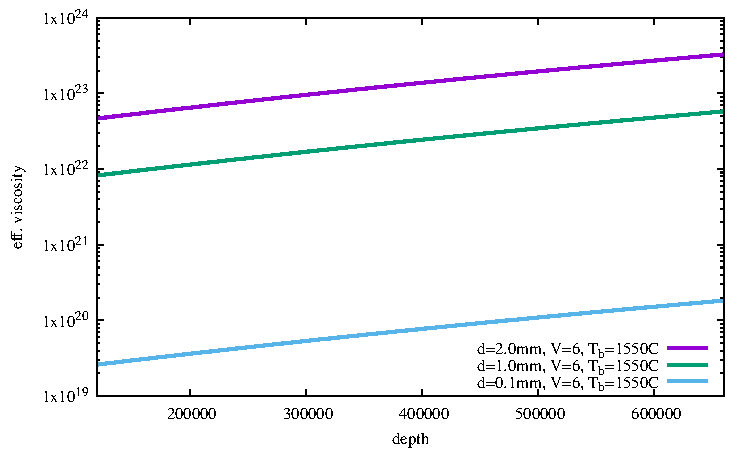
\includegraphics[width=5.cm]{images/rheology/kawudiff/viscosity1.pdf}
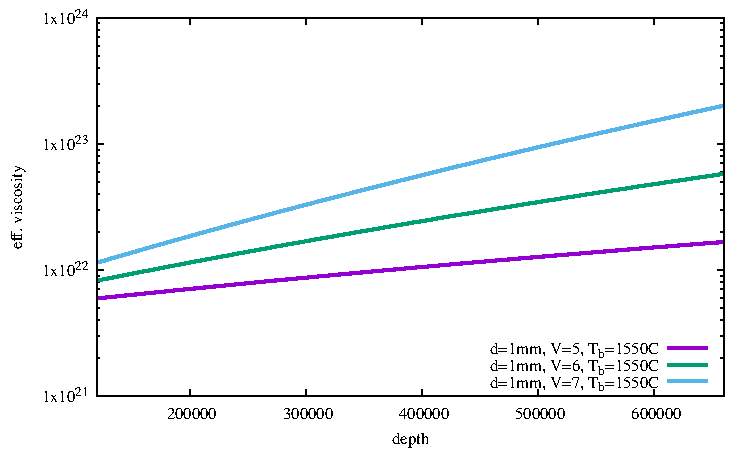
\includegraphics[width=5.cm]{images/rheology/kawudiff/viscosity2.pdf}
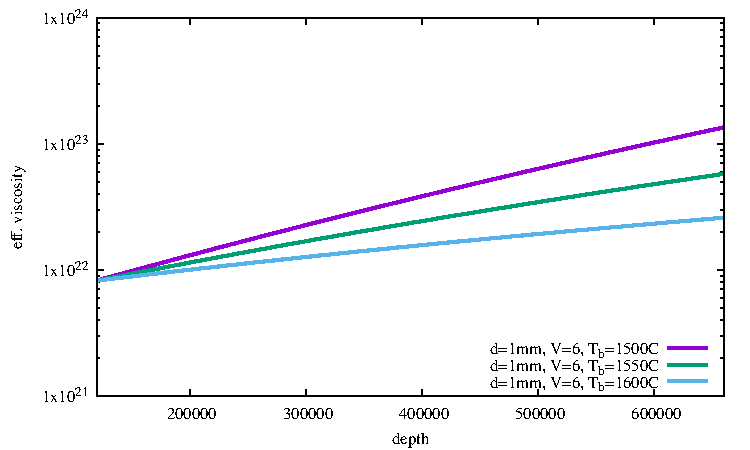
\includegraphics[width=5.cm]{images/rheology/kawudiff/viscosity3.pdf}\\
{\captionfont Effective diffusion creep viscosity for various 
grain size, activation volume and basal temperature values.}\\
{\color{gray} \tiny {images/rheology/kawudiff/}}
\end{center}

Although this exercise only provides us with first-order results, we can conclude that 
one can essentially change the diffusion creep effective viscosity by up to 2 orders of 
magnitude simply by choosing key parameters within acceptable ranges. 

\Literature: \textcite{didu18}\citetitle{didu18}

\newpage
%------------------------------
\subsubsection{The von Mises failure criterion}\label{sec:vMcriterion}
\index{general}{von Mises}

\index{general}{von Mises}
\begin{flushright} {\tiny {\color{gray} vMcriterion.tex}} \end{flushright}
%~~~~~~~~~~~~~~~~~~~~~~~~~~~~~~~~~~~~~~~~~~~~~~~~~~~~~~~~~~~~~~~~~~~~~~~~~~~~~~~~~~~~~~~~~~~~~~~~~~

The von Mises yield criterion suggests that the yielding of materials begins when the second 
deviatoric stress invariant ${\III}_2({\bm \tau})$ reaches a critical value. 
For this reason, it is sometimes called the $J_2$-plasticity or $J_2$ flow 
theory\footnote{$J_2$ is the common notation for ${\III}_2({\bm \tau})$}. 
It is part of a plasticity theory that applies best to ductile materials, such as metals. 

In material science and engineering the von Mises yield criterion can be also formulated in terms of 
the von Mises stress or equivalent tensile stress, $\sigma_v$, a scalar stress value that can be computed 
from the stress tensor. In this case, a material is said to start yielding when its von Mises stress 
reaches a critical value known as the yield strength, $\sigma_Y$. The von Mises stress is used to predict 
yielding of materials under any loading condition from results of simple uniaxial tensile tests. The 
von Mises stress satisfies the property that two stress states with equal distortion energy have equal 
von Mises stress. 

Because the von Mises yield criterion is independent of the first stress 
invariant, ${\III}_1({\bm \sigma})$, it is applicable 
for the analysis of plastic deformation for ductile materials such as metals, as the 
onset of yield for these materials does not depend on the hydrostatic component of the stress tensor. 

Although formulated by Maxwell in 1865, it is generally attributed to von Mises \cite{vonm13}. 
Huber (1904), in a paper in Polish, anticipated to some extent this criterion. 
Heinrich Hencky formulated the same criterion as von Mises independently in 1924 \cite{henc24,tata03}.
This criterion is also referred to as the Maxwell-Huber-Hencky-von Mises theory. 

The von Mises yield criterion (also known as Prandtl-Reuss yield criterion) 
is expressed in the principal stresses as
\[
\sqrt{{\III}_2({\bm \tau})} = c \quad \text{or}, \quad 
\frac{1}{6}[(\sigma_1 - \sigma_2)^2 + (\sigma_2 - \sigma_3)^2 + (\sigma_3 - \sigma_1)^2] =  c^2 
\]
where $c$ is the yield stress in uniaxial tension.
The von Mises yield criterion writes:

\begin{mdframed}[backgroundcolor=blue!5]
\begin{equation}
F^{\text{\tiny VM}}= \sqrt{{\III}_2({\bm \tau})  } - c  \label{vmcrit}
\end{equation}
\end{mdframed}
which is the Drucker-Prager criterion with $\phi=0$ (see Section~\ref{sec:dpcriterion}).

The following figure shows the von Mises yield surface in the three-dimensional space of principal stresses. 
\begin{center}
\includegraphics[width=0.6\textwidth]{images/rheology/vonmises/vonmises.pdf}
\includegraphics[width=0.4\textwidth]{images/rheology/tresca/owenhinton4}\\
{\captionfont Left: Taken from \url{https://en.wikipedia.org/wiki/Yield_surface}.
Right: Taken from \textcite{owhi}.}
\end{center}
It is a circular cylinder of infinite length with its axis inclined at equal angles 
to the three principal stresses. 

\Literature: 
\fullcite{papa87}, \fullcite{ting03}

%\begin{center}
%\includegraphics[width=0.6\textwidth]{RHEOLOGY/viscoplasticity/vMcriterion.pdf}
%\end{center}
\paragraph{The yield surface} Let us try to draw the yield function in 
the space $\sigma_1,\sigma_2,\sigma_3$. It is given by
\begin{eqnarray}
&&\sqrt{ {\III}_2({\bm \tau}) } = c \\
&\Rightarrow&  {\III}_2({\bm \tau})  = c^2 \\
&\Rightarrow& \frac{1}{6}\left[(\sigma_{1}-\sigma_{2})^2 + (\sigma_{2}-\sigma_{3})^2 
+ (\sigma_{1}-\sigma_{3})^2 \right] =c^2 \\
&\Rightarrow & (\sigma_{1}-\sigma_{2})^2 + (\sigma_{2}-\sigma_{3})^2 + (\sigma_{1}-\sigma_{3})^2 = 6c^2 
\end{eqnarray}
or, temporarily setting $x=\sigma_1$, $y=\sigma_2$ and $z=\sigma_3$: 
\begin{eqnarray}
(x-y)^2 + (y-z)^2 + (x-z)^2 &=& 6c^2 \\
(x-y)^2 + y^2 - 2yz + z^2 + x^2 -2xz +z^2 &=& 6c^2\\
2z^2 - 2(x+y)z + (x-y)^2+x^2+y^2-6c^2 &=& 0
\end{eqnarray}
This is a second order polynomial in $z$. Its discriminant $\Delta$ is
\begin{eqnarray}
\Delta 
&=& 4(x+y)^2 - 4 \cdot 2 \cdot [(x-y)^2+x^2+y^2-6c^2] \nn\\
&=& 4x^2 + 8xy + 4y^2 - 8 [x^2-2xy+y^2 +x^2+y^2-6c^2] \nn\\
&=& 4x^2 + 8xy + 4y^2 - 8 [2x^2-2xy+2y^2 -6c^2] \nn\\
&=& 4x^2 + 8xy + 4y^2 - 16x^2+ 16xy -16y^2 +48 c^2 \nn\\
&=& -12x^2 + 24xy -12 y^2  +48 c^2 \nn\\
&=& -12(x^2 -2xy + y^2)  + 48 c^2 \nn\\
&=& -12(x-y)^2  + 48 c^2 \nn
\end{eqnarray}
Since I am looking for $z(x,y)\in \mathbb{R}$ then $\Delta >0$ and this 
imposes a restriction on admissible $x,y$ pairs:
\[
 -12(x-y)^2  + 48 c^2 \nn > 0
\]
\[
(x-y)^2  < 4 c^2 
\]
\[
x-y<2c   
\qquad
\text{or,}
\qquad
y-x<2c   
\]
\[
y> x-2c   
\qquad
\text{or,}
\qquad
y<x+2c
\]
So the discriminant is positive in the band given by $y>x-2c$ and $y<x+2c$ in the $x,y$-plane, 
which is a band centered around the line $y=x$.
When $\Delta>0$ we have then 
\[
z= \frac{2(x+y) \pm \sqrt{\Delta}}{4}
\]
which means that for each pair $x,y$ there are 2 $z$ values. 
The middle of this surface is given by the line $z=(x+y)/2$. 
The plane normal to this line is given by $z=-2(x+y)$.

This approach is reasonably simple for the von Mises criterion but 
quickly becomes intractable for other criteria.

\vspace{.5cm}

We now look into the derivatives of the von Mises plastic potential $Q^{\text{\tiny vM}}(\bm\sigma)$.
We have
\begin{equation}
Q^{\text{\tiny vM}}(\bm\sigma) =\sqrt{{\III}_2({\bm \tau})  } - c  
\end{equation}
Then
\begin{eqnarray}
\frac{\partial Q^{\text{\tiny vM}} }{\partial {\III}_1(\bm\sigma)} &=& 0 \\
\frac{\partial Q^{\text{\tiny vM}} }{\partial \sqrt{{\III}_2(\bm\tau)}}&=& 1 \\
\frac{\partial Q^{\text{\tiny vM}} }{\partial \theta_{\rm L}(\bm\tau)} &=& 0 
\end{eqnarray}
so 
\begin{eqnarray}
C_1^{\text{\tiny vM}} &=& 0  \\ 
C_2^{\text{\tiny vM}} 
&=& \frac{1}{2  \sqrt{{\III}_2(\bm\tau)}   } (1-0) 
= \frac{1}{2  \sqrt{{\III}_2(\bm\tau)}   } \\ 
C_3^{\text{\tiny vM}} &=& 0  
\end{eqnarray}




%------------------------------
\subsubsection{The Tresca failure criterion}\label{sec:trcriterion}
\index{general}{Tresca}

\index{general}{Tresca}
\begin{flushright} {\tiny {\color{gray} trcriterion.tex}} \end{flushright}

The Tresca or maximum shear stress yield criterion is taken to be the work of Henri Tresca. It is also referred as the Tresca-Guest (TG) criterion. The functional form of this yield criterion is
\[
f(\sigma_1,\sigma_2,\sigma_3) = 0
\]
In terms of the principal stresses the Tresca criterion is expressed as
\[
{\max(|\sigma_1 - \sigma_2| , |\sigma_2 - \sigma_3| , |\sigma_3 - \sigma_1| ) = c }
\]
The following figure shows the Tresca-Guest yield surface in the three-dimensional space of principal stresses. 
\begin{center}
\includegraphics[width=0.6\textwidth]{images/rheology/tresca/Tresca.pdf}
\includegraphics[width=0.4\textwidth]{images/rheology/tresca/owenhinton4}\\
{\captionfont Left: Taken from \url{https://en.wikipedia.org/wiki/Yield_surface}.
Right: Taken from \textcite{owhi}.}
\end{center}
It is a prism of six sides and having infinite length. This means that the 
material remains viscous when all three principal stresses are roughly equivalent 
(a hydrostatic pressure), no matter how much it is compressed or stretched. 
However, when one of principal stresses becomes smaller (or larger) than the others 
the material is subject to shearing. In such situations, if the shear 
stress reaches the yield limit then the material enters the plastic domain. 

\begin{remark}
The yield function presents sharp corners, making its numerical implementation 
more difficult (directional derivatives are needed)
\end{remark}

We have already established in Eq.~\eqref{eq:sig13a}:
\begin{eqnarray}
\sigma_1 - \sigma_3  &=& 2 \sqrt{{\cal I}_2({\bm \tau})} \cos \theta \nn
\end{eqnarray}
with $\sigma_1>\sigma_2>\sigma_3$,
so that the failure criterion is given by
\begin{mdframed}[backgroundcolor=blue!5]
\[
F^{\text{\tiny TR}}=2\sqrt{ {\cal I}_2({\bm \tau})  } \cos \theta - c 
\]
\end{mdframed}

\Literature: \fullcite{ting03}

\vspace{.5cm}

We now look into the derivatives of the plastic potential $Q^{\text{\tiny Tr}}(\bm\sigma)$.
We have
\[
Q^{\text{\tiny Tr}}=2\sqrt{ {\cal I}_2({\bm \tau})  } \cos \theta_{\rm L}(\bm\tau) - c
\]

\begin{eqnarray}
\frac{\partial Q^{\text{\tiny Tr}}    }{\partial {\cal I}_1(\bm\sigma)} 
&=& 0 \\
\frac{\partial Q^{\text{\tiny Tr}}    }{\partial \sqrt {{\cal I}_2(\bm\tau)}}
&=& 2 \cos\theta_{\rm L} - 2 \sqrt{ {\cal I}_2({\bm \tau})  } \sin\theta_{\rm L}  
\frac{\partial\theta_{\rm L}}{\partial \sqrt{{\cal I}_2(\bm\tau)}} \nonumber\\
&=& 2 \cos\theta_{\rm L} - 2 \sqrt{ {\cal I}_2({\bm \tau})  } \sin\theta_{\rm L}  
\frac{\partial\theta_{\rm L}}{\partial {{\cal I}_2(\bm\tau)}} 
\frac{\partial {{\cal I}_2(\bm\tau)}}{\partial \sqrt{{\cal I}_2(\bm\tau)}}
\nn\\
&=& 2 \cos\theta_{\rm L} - 2 \sqrt{ {\cal I}_2({\bm \tau})  } \sin\theta_{\rm L}  
\left( -\frac12 \tan 3\theta_{\rm L} \frac{1}{ {\cal I}_2(\bm\tau)}  \right)
2 \sqrt{{\cal I}_2(\bm\tau)}
\nn\\
&=& 2 \cos\theta_{\rm L} +  2 \sin\theta_{\rm L}  
\tan 3\theta_{\rm L} 
\nn\\
&=& 2 \cos\theta_{\rm L} ( 1 + \tan\theta_{\rm L}  \tan 3\theta_{\rm L}) \\
\frac{\partial Q^{\text{\tiny Tr}} }{\partial \theta_{\rm L}(\bm\tau)} 
&=& 
-2\sqrt{ {\cal I}_2({\bm \tau})  } \sin \theta_{\rm L} 
\end{eqnarray}

so
\begin{eqnarray}
C_1^{\text{\tiny Tr}} &=& 0 \\ 
C_2^{\text{\tiny Tr}} 
&=& \frac{1}{2 \sqrt{ {\cal I}_2(\bm\tau)}   }   
\left( \frac{\partial Q}{\partial \sqrt{{\cal I}_2(\bm\tau)}} 
- \frac{\tan 3\theta_{\rm L}}{\sqrt {{\cal I}_2(\bm\tau)}}
\frac{\partial Q}{\partial \theta_{\rm L}(\bm\tau)}  
\right) \nn\\
&=&
\frac{1}{2 \sqrt{ {\cal I}_2(\bm\tau)}   }   
\left( 2 \cos\theta_{\rm L} ( 1 + \tan\theta_{\rm L}  \tan 3\theta_{\rm L})
+ \frac{\tan 3\theta_{\rm L}}{\sqrt {{\cal I}_2(\bm\tau)}}
2\sqrt{ {\cal I}_2({\bm \tau})  } \sin \theta_{\rm L} 
\right) \nn\\
&=&
\frac{1}{2 \sqrt{ {\cal I}_2(\bm\tau)}   }   
\left( 2 \cos\theta_{\rm L} ( 1 + \tan\theta_{\rm L}  \tan 3\theta_{\rm L})
+ 2 \tan 3\theta_{\rm L} \sin \theta_{\rm L} \right) \nn\\
&=&
\frac{1}{2 \sqrt{ {\cal I}_2(\bm\tau)}   }   
\left( 2 \cos\theta_{\rm L} ( 1 + \tan\theta_{\rm L}  \tan 3\theta_{\rm L})
+ 2 \cos\theta_{\rm L} \tan 3\theta_{\rm L}  \tan \theta_{\rm L} 
\right) \nn\\
&=&
\frac{1}{2 \sqrt{ {\cal I}_2(\bm\tau)}   }   
\left( 2 \cos\theta_{\rm L} ( 1 + 2 \tan\theta_{\rm L}  \tan 3\theta_{\rm L}) \right) \\
C_3^{\text{\tiny Tr}} 
&=&  - \frac{\sqrt{3}}{2\cos 3\theta_{\rm L}}
\frac{1}{{\cal I}_2(\bm\tau)^{3/2}} 
\frac{\partial Q}{\partial \theta_{\rm L}(\bm\tau)} \nn\\
&=&  -
\frac{\sqrt{3}}{2\cos 3\theta_{\rm L}}
\frac{1}{{\cal I}_2(\bm\tau)^{3/2}} 
(-2\sqrt{ {\cal I}_2({\bm \tau})  } \sin \theta_{\rm L} ) \nn\\
&=& \frac{\sqrt{3}}{{\cal I}_2({\bm \tau}) }
\frac{\sin\theta_{\rm L} }{\cos 3\theta_{\rm L}}
\end{eqnarray}































%DO NOT READ FURTHER - 9dec2019
%%%%%%%%%%%%%%%%%%%%%%%%%%%%%%%%%%
%Using the values of the principal stresses in a two dimensional space, the criterion becomes 
%\[
%|\sigma_1 - \sigma_2| =\sqrt{J_2'}  = \sigma_0 
%\]
%which is equivalent to the von Mises criterion.


\newpage


%------------------------------
\subsubsection{The Mohr-Coulomb failure criterion}\label{sec:mccriterion}
\index{general}{Mohr-Coulomb}
\index{general}{Mohr-Coulomb}
\begin{flushright} {\tiny {\color{gray} mccriterion.tex}} \end{flushright}
%~~~~~~~~~~~~~~~~~~~~~~~~~~~~~~~~~~~~~~~~~~~~~~~~~~~~~~~~~~~~~~~~~~~~~~~~~~~~~~~~~~~~~~~~~~~~~~~~~~

Mohr-Coulomb theory is a model describing the response of a material such as rubble piles or concrete to shear stress as well as normal stress. 
Most of the classical engineering materials somehow follow this rule in at least a portion of their shear failure envelope. In geology it is used to define shear strength of soils at different effective stresses \cite{hand69}.

In structural engineering it is used to determine failure load as well as the angle of fracture of a displacement fracture in concrete and similar materials. Coulomb's friction hypothesis is used to determine the combination of shear and normal stress that will cause a fracture of the material. Mohr's circle is used to determine the principal stresses that will produce this combination of shear and normal stress, and the angle of the plane in which this will occur. According to the principle of normality, the stress introduced at failure will be perpendicular to the line describing the fracture condition.

%It can be shown that a material failing according to Coulomb's friction hypothesis will show the displacement introduced at failure forming an angle to the line of fracture equal to the angle of friction. This makes the strength of the material determinable by comparing the external mechanical work introduced by the displacement and the external load with the internal mechanical work introduced by the strain and stress at the line of failure. By conservation of energy the sum of these must be zero and this will make it possible to calculate the failure load of the construction.

\begin{center}
\includegraphics[width=6cm]{images/rheology/owenhinton5}\\
{\captionfont Taken from \textcite{owhi}.}
\end{center}

The Mohr-Coulomb failure criterion represents the linear envelope that is obtained 
from a plot of the shear strength of a material 
versus the applied normal stress. This relation is expressed as (Owen \& Hinton book \cite[p219]{owhi})
%\[
%\tau = c- \sigma~\tan(\phi) 
%\]

%Compression is assumed to be positive in the following discussion. If compression is assumed to be negative then $\sigma$ should be replaced with $-\sigma$.

%If $\phi=0$, the Mohr-Coulomb criterion reduces to the Tresca criterion. On the other hand, if $\phi = 90^\circ$ the Mohr-Coulomb model is equivalent to the Rankine model. Higher values of $\phi$ are not allowed.

\begin{equation}
\tau_m = -\sigma_m \sin \phi + c \cos \phi  \label{eq:mccrit}
\end{equation}
where $\tau_m$ is the magnitude of the shear stress, 
$\sigma_m$ is the normal stress, $c$ is the intercept of the failure envelope with the $\tau$ axis, 
and $\phi$ is the slope of the failure envelope.
The minus sign in the above equation is for the case where compression is assumed to be 
negative\footnote{\url{https://en.wikipedia.org/wiki/Mohr-Coulomb_theory}}.
The quantity $c$ is often called the cohesion and the angle $\phi$ is called the angle of internal friction.
 
We have  
\[
\tau_m=\frac{\sigma_1-\sigma_3}{2}
\qquad
\qquad
\sigma_m = \frac{\sigma_1+\sigma_3}{2}
\]
with $\sigma_1$ is the maximum principal stress and $\sigma_3$ is the minimum principal stress, or
%\[
%\sigma_1-\sigma_3 = - ( \sigma_1+\sigma_3) \sin \phi + 2c \cos \phi
%\]
%\[
%\sigma_1-\sigma_3 = 2 c \cos \phi - (\sigma_1+\sigma_3) \sin\phi
%\]
\begin{equation}
\cfrac{\sigma_1-\sigma_3}{2} = -\cfrac{\sigma_1+\sigma_3}{2}~\sin\phi +c\; \cos\phi 
\end{equation}
Using Eqs.~\eqref{eq:sig13a} and \eqref{eq:sig13b} 
for $(\sigma_1 - \sigma_3 )/2$ and $(\sigma_1 + \sigma_3 )/2$ we get\footnote{This is 
Eq.~(7.16) of \textcite{owhi}}:
\begin{eqnarray}
&& \frac{\sigma_1 - \sigma_3}{2} = -\frac{\sigma_1 + \sigma_3}{2} \sin \phi  + c \cos \phi \nn\\
&\Rightarrow&
\sqrt{  {\III}_2({\bm \tau}) } \cos \theta = -\left(\frac{1}{3}{\III}_1({\bm \sigma}) - \sqrt{  {\III}_2({\bm \tau})} \frac{1}{\sqrt{3}} \sin \theta \right) \sin \phi 
+ c \cos \phi \nn\\
&\Rightarrow&
\frac{1}{3} {\III}_1({\bm \sigma}) \sin \phi  
+ \sqrt{  {\III}_2({\bm \tau}) } \left( \cos \theta - \frac{1}{\sqrt{3}} \sin \theta  \sin \phi \right) - c \cos \phi = 0 \nn
\end{eqnarray}

\begin{mdframed}[backgroundcolor=blue!5]
\begin{equation}
F^{\text{\tiny MC}}=\frac{1}{3} {\III}_1({\bm \sigma}) \sin \phi  + 
\sqrt{  {\III}_2({\bm \tau})  } \left( \cos \theta - \frac{1}{\sqrt{3}} \sin \theta  \sin \phi \right) - c \cos \phi
\label{eq:mcF} 
\end{equation}
\end{mdframed}
This formula (without the cohesion) is used in \textcite{will92}.
Since $p=-\frac{1}{3} {\III}_1({\bm \sigma})$, we also have:
%\begin{equation}
%F^{\text{\tiny MC}}= -p \sin \phi  + 
%\sqrt{ {\III}_2({\bm \tau})  } \left( \cos \theta - \frac{1}{\sqrt{3}} \sin \theta  \sin \phi \right) - c \cos \phi 
%\end{equation}
%or, 
\begin{mdframed}[backgroundcolor=blue!5]
\begin{equation}
F^{\text{\tiny MC}}=
\sqrt{  {\III}_2({\bm \tau})  } \left( \cos \theta - \frac{1}{\sqrt{3}} \sin \theta  \sin \phi \right) - (p \sin\phi + c \cos \phi)
\end{equation}
\end{mdframed}

\begin{remark}
The expression for $F$ in the Mohr-Coulomb case in Zienkiewicz \& Cormeau (1974) \cite{zico74} 
contains errors which are later corrected in \textcite[p102]{book_zitf}. 
\end{remark}

\Literature: this criterion is also used in computer graphics animation \cite{zhbr05}

\todo{when $\phi=0$ we should recover Tresca but factor 2 is wrong ?}



\vspace{.5cm}

We now look into the derivatives of the Drucker-Prager plastic potential $Q^{\text{\tiny MC}}(\bm\sigma)$.
We have
\[
Q^{\text{\tiny MC}}=
\frac{1}{3} {\III}_1({\bm \sigma}) \sin \phi  + 
\sqrt{  {\III}_2({\bm \tau})  } \left(\cos\theta_{\rm L}(\bm\tau)-\frac{1}{\sqrt{3}} 
\sin\theta_{\rm L} (\bm\tau) \sin\phi \right) -c \cos \phi
\]
Then
\begin{eqnarray}
\frac{\partial Q^{\text{\tiny MC}}  }{\partial {\III}_1(\bm\sigma)} &=& \frac13 \sin\phi \\
\frac{\partial Q^{\text{\tiny MC}}  }{\partial \sqrt {{\III}_2(\bm\tau)}}
&=&  
\cos \theta_{\rm L} - \frac{1}{\sqrt{3}} \sin \theta_{\rm L}  \sin \phi  
+  \sqrt{  {\III}_2({\bm \tau})  } 
\left(-\sin \theta_{\rm L} - \frac{1}{\sqrt{3}} \cos \theta_{\rm L}  \sin \phi \right) 
\frac{\partial \theta_{\rm L}}{\partial \sqrt {{\III}_2(\bm\tau)}   } \nn \\
&=&  
\cos \theta_{\rm L} - \frac{1}{\sqrt{3}} \sin \theta_{\rm L}  \sin \phi  
+  \sqrt{  {\III}_2({\bm \tau})  } 
\left(-\sin \theta_{\rm L} - \frac{1}{\sqrt{3}} \cos \theta_{\rm L}  \sin \phi \right) 
\frac{\partial \theta_{\rm L}}{\partial  {{\III}_2(\bm\tau)}   }  
\frac{\partial   {{\III}_2(\bm\tau)}     }{\partial \sqrt {{\III}_2(\bm\tau)}   }  \nn\\
&=&  
\cos \theta_{\rm L} - \frac{1}{\sqrt{3}} \sin \theta_{\rm L}  \sin \phi  
+  \sqrt{  {\III}_2({\bm \tau})  } 
\left(-\sin \theta_{\rm L} - \frac{1}{\sqrt{3}} \cos \theta_{\rm L}  \sin \phi \right) 
\left(
-\frac12 \tan 3\theta_{\rm L} \frac{1}{ {\III}_2(\bm\tau)} 
\right)
2 \sqrt {{\III}_2(\bm\tau)} \nn \\
&=&  
\cos \theta_{\rm L} - \frac{1}{\sqrt{3}} \sin \theta_{\rm L}  \sin \phi  
+  
\left(\sin \theta_{\rm L} + \frac{1}{\sqrt{3}}\cos\theta_{\rm L}\sin\phi\right) \tan 3\theta_{\rm L} \nn\\
&=&  
\cos \theta_{\rm L}
\left[
1 - \frac{1}{\sqrt{3}} \tan \theta_{\rm L}  \sin \phi  
+  
\left(\tan \theta_{\rm L} + \frac{1}{\sqrt{3}}   \sin \phi \right)  \tan 3\theta_{\rm L} 
\right] \nn\\
&=&
\cos \theta_{\rm L}
\left[
(1 +  \tan \theta_{\rm L}   \tan 3\theta_{\rm L})
+\frac{1}{\sqrt{3}} \sin\phi
( \tan 3\theta_{\rm L} - \tan\theta_{\rm L})
\right]
\\ 
\frac{\partial Q^{\text{\tiny MC}} }{\partial \theta_{\rm L}(\bm\tau)} 
&=&  
\sqrt{{\III}_2(\bm \tau)} (-\sin\theta_{\rm L}-\frac{1}{\sqrt{3}} \cos\theta_{\rm L} \sin\phi )\nn\\
&=&  
-\frac{1}{\sqrt{3}} \sqrt{{\III}_2(\bm \tau)} (\sqrt{3} \sin\theta_{\rm L}+\cos\theta_{\rm L} \sin\phi )
\end{eqnarray}
so
\begin{eqnarray}
C_1^{\text{\tiny MC}} &=& \frac13 \sin\phi  \\ 
C_2^{\text{\tiny MC}} 
&=& 
\frac{1}{2 \sqrt{ {\III}_2(\bm\tau)}   }   
\left( \frac{\partial Q}{\partial \sqrt{{\III}_2(\bm\tau)}} 
- \frac{\tan 3\theta_{\rm L}}{\sqrt {{\III}_2(\bm\tau)}}
\frac{\partial Q}{\partial \theta_{\rm L}(\bm\tau)}  
\right) \nn\\
&=& 
\frac{1}{2 \sqrt{ {\III}_2(\bm\tau)}   }   
\left( \cos \theta_{\rm L} \left[
(1 +  \tan \theta_{\rm L}   \tan 3\theta_{\rm L})
+\frac{1}{\sqrt{3}} \sin\phi ( \tan 3\theta_{\rm L} - \tan\theta_{\rm L}) \right]
+ \frac{\tan 3\theta_{\rm L}}{\sqrt {{\III}_2(\bm\tau)}}
\frac{1}{\sqrt{3}} \sqrt{{\III}_2(\bm \tau)} (\sqrt{3} \sin\theta_{\rm L}+\cos\theta_{\rm L} \sin\phi )
\right) \nn\\
&=& 
\frac{1}{2 \sqrt{ {\III}_2(\bm\tau)}   }   
\left( \cos \theta_{\rm L}
\left[ (1 +  \tan \theta_{\rm L}   \tan 3\theta_{\rm L})
+\frac{1}{\sqrt{3}} \sin\phi
( \tan 3\theta_{\rm L} - \tan\theta_{\rm L}) \right]
+ \tan 3\theta_{\rm L}  ( \sin\theta_{\rm L}+\frac{1}{\sqrt{3}}\cos\theta_{\rm L} \sin\phi )
\right) \nn\\
&=& 
\frac{1}{2 \sqrt{ {\III}_2(\bm\tau)}   }   
\left( \cos \theta_{\rm L} \left[
(1 +  \tan \theta_{\rm L}   \tan 3\theta_{\rm L})
+\frac{1}{\sqrt{3}} \sin\phi
( \tan 3\theta_{\rm L} - \tan\theta_{\rm L})
+ \tan 3\theta_{\rm L}   ( \tan\theta_{\rm L}+\frac{1}{\sqrt{3}} \sin\phi )
\right] \right) \nn\\
&=& 
\frac{1}{2 \sqrt{ {\III}_2(\bm\tau)}   }   
\cos \theta_{\rm L} \left[
(1 +  2\tan \theta_{\rm L}   \tan 3\theta_{\rm L})
+\frac{1}{\sqrt{3}} \sin\phi ( 2\tan 3\theta_{\rm L} - \tan\theta_{\rm L})
\right] \nn\\
C_3^{\text{\tiny MC}} 
&=&  - \frac{\sqrt{3}}{2\cos 3\theta_{\rm L}}
\frac{1}{{\III}_2(\bm\tau)^{3/2}} 
\frac{\partial Q}{\partial \theta_{\rm L}(\bm\tau)} \nn\\ 
&=&  - \frac{\sqrt{3}}{2\cos 3\theta_{\rm L}}
\frac{1}{{\III}_2(\bm\tau)^{3/2}} 
\left[-\frac{1}{\sqrt{3}} \sqrt{{\III}_2(\bm \tau)} (\sqrt{3} \sin\theta_{\rm L}+\cos\theta_{\rm L} 
\sin\phi ) \right]  \nn\\
&=&  \frac{\sqrt{3}\sin\theta_{\rm L} +  \sin \phi \cos \theta_{\rm L}}
{2 {\III}_2({\bm \tau}) \cos 3\theta_{\rm L}}
\end{eqnarray}










%\newpage
%\paragraph{two-dimensional space}

%The principal stress values are given by
%\[
%\sigma_{1,3} = \frac{\sigma_{xx}+\sigma_{yy}}{2} \pm \sqrt{ \frac{1}{4}(\sigma_{xx}-\sigma_{yy})^2 + \sigma_{xy}^2  }
%= \frac{J_1}{2} \pm \sqrt{ J_2'}
%\]
%so
%\[
%\frac{\sigma_1-\sigma_3}{2} = \frac{\sqrt{J_2}- - \sqrt{J_2}}{2} = \sqrt{J_2}
%\]
%\[
%\frac{\sigma_1+\sigma_3}{2} =  \frac{J_1}{2} 
%\]
%and then
%\[
%\sqrt{J_2} = - \frac{J_1}{2} \sin\phi + c\cos\phi 
%\]
%The Mohr-Coulomb criterion simply writes:
%
%\begin{mdframed}[backgroundcolor=blue!5]
%\begin{equation}
%F^{MC,2D}=  \frac{J_1}{2} \sin \phi + \sqrt{J_2} - c  \cos \phi  \label{mc2Dcriterion}
%\end{equation}
%\end{mdframed}

%%%%%%%%%%%%%%%%%%%%%%%%%%%%%%%%%%%%
%\paragraph{three-dimensional space}
%The Haigh-Westergaard invariants are related to the principal stresses by
%\begin{eqnarray}
%\sigma_1 &=& \cfrac{1}{\sqrt{3}}~\xi + \sqrt{\cfrac{2}{3}}~\rho~\cos\theta  \nonumber\\
%\sigma_3 &=& \cfrac{1}{\sqrt{3}}~\xi + \sqrt{\cfrac{2}{3}}~\rho~\cos\left(\theta+\cfrac{2\pi}{3}\right) \nonumber
%\end{eqnarray}
%Plugging into the expression for the Mohr-Coulomb yield function gives us
%\[
% -\sqrt{2}~\xi~\sin\phi + \rho[\cos\theta - \cos(\theta+2\pi/3)] - \rho\sin\phi[\cos\theta+\cos(\theta+2\pi/3)] = \sqrt{6}~c~\cos\phi 
%\]
%Using trigonometric identities for the sum and difference of cosines and rearrangement gives us the expression of the Mohr-Coulomb yield function in terms of $\xi$, $\rho$ and $\theta$:
%\[
%\left[\sqrt{3}~\sin\left(\theta+\cfrac{\pi}{3}\right) - \sin\phi\cos\left(\theta+\cfrac{\pi}{3}\right)\right]\rho - \sqrt{2}\sin(\phi)\xi = \sqrt{6} c \cos\phi 
%\]
%Alternatively, in terms of the invariants $p$,$q$,$r$ we can write
%\[
%\left[\cfrac{1}{\sqrt{3}~\cos\phi}~\sin\left(\theta+\cfrac{\pi}{3}\right) - \cfrac{1}{3}\tan\phi~\cos\left(\theta+\cfrac{\pi}{3}\right)\right]q - p~\tan\phi = c 
%\]

\newpage


%------------------------------
\subsubsection{The Drucker-Prager failure criterion \label{sec:dpcriterion}}
\index{general}{Drucker-Prager}
\index{general}{Drucker-Prager}
\begin{flushright} {\tiny {\color{gray} dpcriterion.tex}} \end{flushright}
%~~~~~~~~~~~~~~~~~~~~~~~~~~~~~~~~~~~~~~~~~~~~~~~~~~~~~~~~~~~~~~~~~~~~~~~~~~~~~~~~~~~~~~~~~~~~~~~~~~

The von Mises yield criterion is not suitable for modelling the yielding of frictional material 
as it does not include the effect of mean stress as observed in experiments. To overcome this 
limitation, Drucker and Prager (1952) \cite{drpr52} proposed a revised function for frictional materials.

The Drucker-Prager yield criterion has the function form
\begin{equation}
\FFF^{\text{\tiny DP}}({\bm \sigma})=\FFF \left( {\cal I}_1({\bm \sigma}), {\cal I}_2({\bm \tau}) \right) = 0 
\end{equation}
This criterion is most often used for concrete where both normal and shear stresses 
can determine failure. The Drucker-Prager yield criterion may be expressed as
\begin{mdframed}[backgroundcolor=blue!5]
\begin{equation}
\FFF^{\text{\tiny DP}}= \sqrt{{\cal I}_2({\bm \tau})} + \alpha {\cal I}_1({\bm \sigma}) + k =0  
\label{dpcriterion} 
\end{equation}
\end{mdframed}

{\color{orange} it should probably be -k .. this needs to be propagated below!}

The problem is then to choose $\alpha$ and $k$ in a meaningful way, typically in relation with the 
Mohr-Coulomb criterion.

\begin{center}
\includegraphics[width=9cm]{images/rheology/owenhinton5}\\
{\captionfont Taken from \textcite{owhi}. The Drucker-Prager yield envelope 
circumscribes the Mohr-Coulomb one.}
\end{center}

Using the parameters $\sigma_m$, $\tau_m$, $a=-\sqrt{3}\tan\uptheta$, ${\cal I}_1({\bm \sigma})$ 
and ${\cal I}_2({\bm \tau})$ of Section~\ref{sec:altinv} we have
\begin{eqnarray}
\FFF^{\text{\tiny DP}}
&=&  \sqrt{{\cal I}_2({\bm \tau})} + \alpha {\cal I}_1({\bm \sigma}) + k \nn\\
&=& \sqrt{\frac{\tau_m^2}{3}(a^2+3)} + \alpha (3\sigma_m-a\tau_m) + k \nn\\ 
&=& \tau_m \sqrt{(a^2/3+1)} + \alpha (3\sigma_m+\tau_m\sqrt{3}\tan\uptheta ) + k    \qquad ({\rm since }\; \tau_m>0)\nn\\ 
&=& \tau_m \sqrt{\tan^2\uptheta+1} + \alpha (3\sigma_m+\tau_m\sqrt{3}\tan\uptheta ) + k  \nn\\
&=& \tau_m \sqrt{ \frac{1}{\cos^2\uptheta} } + \alpha (3\sigma_m+\tau_m\sqrt{3}\tan\uptheta ) + k  \nn\\
&=& \tau_m \frac{1}{\cos\uptheta} +\alpha (3\sigma_m+\tau_m\sqrt{3}\tan\uptheta ) + k  \qquad ({\rm since }\; \cos\uptheta >0)\nn
\end{eqnarray}
$\FFF^{\text{\tiny DP}}=0$ then leads to write
\begin{eqnarray}
\tau_m  + (3 \alpha \sigma_m+k)\cos\uptheta  + \tau_m \alpha \sqrt{3}\sin\uptheta  &=&0 \nn\\
\Rightarrow \qquad \tau_m(1 + \alpha \sqrt{3}\sin\uptheta)  + (3 \alpha \sigma_m+k)\cos\uptheta &=&0 \nn
\end{eqnarray}
and finally
\[
\tau_m = -\frac{(3 \alpha \sigma_m+k)\cos\uptheta}{1 + \alpha \sqrt{3}\sin\uptheta}
= -\frac{3 \alpha \cos\uptheta}{1 + \alpha \sqrt{3}\sin\uptheta} \sigma_m 
-\frac{k\cos\uptheta}{1 + \alpha \sqrt{3}\sin\uptheta}
\]
\begin{remark}
This is the same equation as Eq.~19 of Wojciechowski \cite{wojc18} but with $\uptheta \rightarrow -\uptheta$. 
\end{remark}

\vspace{.5cm}

The Mohr-Coulomb yield criterion is  (see Eq.~\eqref{eq:mccrit})
\[
\tau_m = -\sigma_m \sin\phi + c \cos\phi
\]
so that equating both expressions of $\tau_m$ for the Drucker-Prager 
and Mohr-Coulomb criteria leads to:
\begin{eqnarray}
-\frac{3 \alpha \cos\uptheta}{1 + \alpha \sqrt{3}\sin\uptheta} &=& -\sin\phi \label{eq:qq1}\\
-\frac{k\cos\uptheta}{1 + \alpha \sqrt{3}\sin\uptheta} &=& c \cos\phi \label{eq:qq2}
\end{eqnarray}
Eq.~\eqref{eq:qq1} yields
\[
3 \alpha \cos\uptheta = \sin\phi (1 + \alpha \sqrt{3}\sin\uptheta) 
\]
\[
\Rightarrow \qquad 3 \alpha \cos\uptheta - \alpha \sqrt{3}\sin\uptheta \sin\phi = \sin\phi 
\]
and finally 
\begin{equation}
\boxed{
\alpha(\phi) =  \frac{\sin\phi}{ 3 \cos\uptheta - \sqrt{3}\sin\uptheta \sin\phi}
}
\label{eq:dpalpha}
\end{equation}
Inserting this into Eq.~\eqref{eq:qq2}:
\begin{eqnarray}
- k \cos\uptheta 
&=& c \cos \phi \left(1 +\alpha \sqrt{3} \sin\uptheta \right)  \nn\\
&=& c \cos \phi \left(1 + \frac{\sin\phi}{ 3 \cos\uptheta - \sqrt{3}\sin\uptheta \sin\phi}  \sqrt{3} \sin\uptheta\right) \nn\\
&=& c \cos \phi \left(1 + 
\frac{ \sqrt{3}\sin\phi \sin\uptheta }{ 3 \cos\uptheta - \sqrt{3}\sin\uptheta \sin\phi} \right) \nn\\
&=& c \cos \phi \left(
\frac{ 3 \cos\uptheta - \sqrt{3}\sin\uptheta \sin\phi}{ 3 \cos\uptheta - \sqrt{3}\sin\uptheta \sin\phi} 
+ 
\frac{ \sqrt{3}\sin\phi \sin\uptheta }{ 3 \cos\uptheta - \sqrt{3}\sin\uptheta \sin\phi} \right) \nn\\
&=& c \cos \phi \left(
\frac{ 3 \cos\uptheta}{ 3 \cos\uptheta - \sqrt{3}\sin\uptheta \sin\phi} \right) \nn
\end{eqnarray}
so that 
\begin{equation}
\boxed{
k(c,\phi) =- \frac{ 3\; c \cos \phi }{ 3 \cos\uptheta - \sqrt{3}\sin\uptheta \sin\phi} 
}
\label{eq:dpk}
\end{equation}
%Unsurprisingly we recover the Eqs. 20 and 21 of Wojciechowski \cite{wojc18} by replacing $\theta$ by $-\theta$.

The Drucker-Prager yield criterion which for a given $\theta$ is equal to the Mohr-Coulomb yield is then:
\begin{eqnarray}
\FFF^{\text{\tiny DP}}
&=& \sqrt{{\cal I}_2({\bm \tau})} + \alpha(\phi) {\cal I}_1({\bm \sigma}) + k(c,\phi)  \nn\\
&=& \sqrt{{\cal I}_2({\bm \tau})} 
+ \frac{\sin\phi}{ 3 \cos\uptheta - \sqrt{3}\sin\uptheta \sin\phi}  {\cal I}_1({\bm \sigma})  
- \frac{ 3\; c \cos \phi }{ 3 \cos\uptheta - \sqrt{3}\sin\uptheta \sin\phi} \nn\\
&=& \sqrt{{\cal I}_2({\bm \tau})} 
- \left[ -\frac{3 \sin\phi}{ 3 \cos\uptheta - \sqrt{3}\sin\uptheta \sin\phi}  \frac{{\cal I}_1({\bm \sigma})}{3}
+ \frac{ 3\; c \cos \phi }{ 3 \cos\uptheta - \sqrt{3}\sin\uptheta \sin\phi} \right] \label{eq:Fdp}\\
&=& \sqrt{{\cal I}_2({\bm \tau})} 
- \left[ \frac{3\; p \sin\phi}{ 3 \cos\uptheta - \sqrt{3}\sin\uptheta \sin\phi} 
+ \frac{ 3\; c \cos \phi }{ 3 \cos\uptheta - \sqrt{3}\sin\uptheta \sin\phi} \right] \nn\\
&=& \sqrt{{\cal I}_2({\bm \tau})}  
- \frac{3\; p \sin\phi  + 3\; c \cos \phi }{ 3 \cos\uptheta - \sqrt{3}\sin\uptheta \sin\phi} \nn\\ 
&=& \sqrt{{\cal I}_2({\bm \tau})}  
- \frac{p \sin\phi  + c \cos \phi }{  \cos\uptheta - \frac{1}{\sqrt{3}}\sin\uptheta \sin\phi} 
\end{eqnarray}
which, when multiplied by $\cos\uptheta - \frac{1}{\sqrt{3}}\sin\uptheta \sin\phi$, gives
the Mohr-Coulomb criterion of Eq.~\eqref{eq:mcF}. 

%------------------------------------
\subsection{The three standard types}

For $\uptheta=\pi/6$, the DP yield surface {\bf circumscribes} the MC yield 
surface and Eq.~\eqref{eq:Fdp} writes:
\begin{eqnarray}
\FFF^{\text{\tiny DP}}
&=& \sqrt{{\cal I}_2({\bm \tau})} 
- \left[ -\frac{3 \sin\phi}{ 3 \sqrt{3}/2 - \sqrt{3}/2 \; \sin\phi}  \frac{{\cal I}_1({\bm \sigma})}{3}
+ \frac{ 3\; c \cos \phi }{ 3 \sqrt{3}/2 - \sqrt{3}/2 \; \sin\phi} \right] \nn\\
&=& \sqrt{{\cal I}_2({\bm \tau})} 
- \left[ -\frac{6 \sin\phi}{\sqrt{3} (3 - \sin\phi) }  \frac{{\cal I}_1({\bm \sigma})}{3}
+ \frac{ 6\; c \cos \phi }{ \sqrt{3}(3 - \sin\phi)} \right] \nn\\
&=& \sqrt{{\cal I}_2({\bm \tau})} 
- \frac{ 6 p \sin \phi + 6\; c \cos \phi }{ \sqrt{3}(3 - \sin\phi)} \label{eq:dpc}
\end{eqnarray}
i.e.

\begin{center}
\includegraphics[width=8cm]{images/rheology/owenhinton6}\\
{\captionfont Taken from \textcite{owhi}.}
\end{center}

\begin{mdframed}[backgroundcolor=blue!5]
\begin{equation}
\FFF^{\text{\tiny DP}}
= \sqrt{{\cal I}_2({\bm \tau})} 
+ \frac{ 6 \sin \phi }{ \sqrt{3}(3 - \sin\phi)} \frac{{\cal I}_1({\bm\sigma})}{3}
- \frac{ 6\; c \cos \phi }{ \sqrt{3}(3 - \sin\phi)} 
\end{equation}
\end{mdframed}

which is the formula used in Glerum \etal (2018) \cite{gltf18}.
This is also Eq.~(14a) in Zienkiewicz \& Cormeau (1974) \cite{zico74}, 
Eq.~(7.18) in \textcite{owhi}, and Eq.~(13.10a) in Zienkiewicz (1975) \cite{zien75} 
provided it is divided altogether by $\sqrt 3$. 


For $\uptheta=-\pi/6$, the DP yield surface {\bf middle circumscribes} the MC yield surface 
and Eq.~\eqref{eq:Fdp} writes:
\begin{eqnarray}
\FFF^{\text{\tiny DP}}
&=& \sqrt{{\cal I}_2({\bm \tau})} 
- \left[ -\frac{3 \sin\phi}{ 3 \sqrt{3}/2 + \sqrt{3}/2 \sin\phi}  \frac{{\cal I}_1({\bm \sigma})}{3}
+ \frac{ 3\; c \cos \phi }{ 3 \sqrt{3}/2 + \sqrt{3}/2 \sin\phi} \right] \nn\\
&=& \sqrt{{\cal I}_2({\bm \tau})} 
- \left[ -\frac{6 \sin\phi}{\sqrt{3} (3 + \sin\phi) }  \frac{{\cal I}_1({\bm \sigma})}{3}
+ \frac{ 6\; c \cos \phi }{ \sqrt{3}(3 + \sin\phi}) \right] \nn\\
&=& \sqrt{{\cal I}_2({\bm \tau})} 
- \frac{6 p \sin\phi + 6 c \cos \phi}{\sqrt{3} (3 + \sin\phi) } 
\end{eqnarray}
This is Eq.~(7.19) of \textcite{owhi}.

Another DP formulation which {\bf inscribes} the MC yield surface is found on the 
wikipedia page of the Drucker-Prager yield criterion
\footnote{\url{https://en.wikipedia.org/wiki/Drucker-Prager_yield_criterion}. 
(but I have no idea how it is arrived at)}\todo{Look into it!}:

\begin{center}
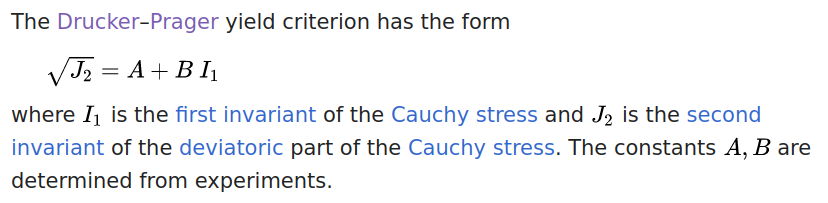
\includegraphics[width=9cm]{images/rheology/dp_wiki1}\\
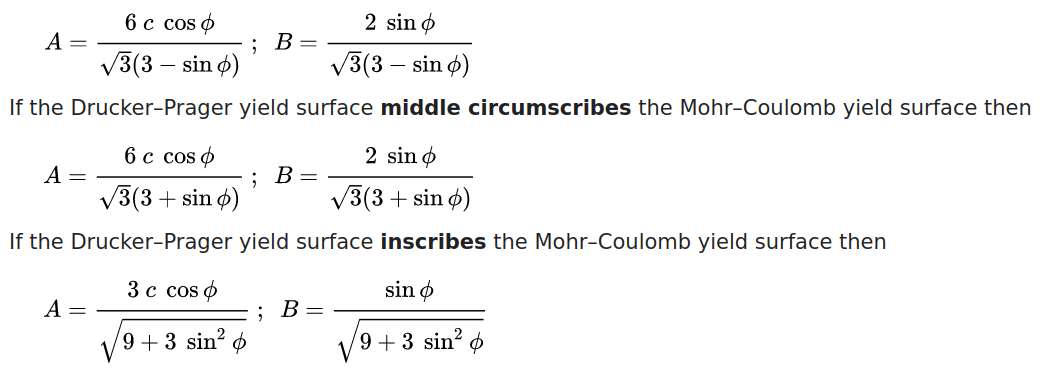
\includegraphics[width=9cm]{images/rheology/dp_wiki2}\\
\end{center}

With our notations:

\begin{eqnarray}
\FFF^{\text{\tiny DP}}
&=& \sqrt{{\cal I}_2({\bm \tau})} 
- \left[ -\frac{3 \sin\phi}{\sqrt{9+3\sin^2\phi} }  \frac{{\cal I}_1({\bm \sigma})}{3}
+ \frac{ 3\; c \cos \phi }{ \sqrt{9+3\sin^2\phi} } \right] \label{eq:dp3}
\end{eqnarray}

The yield surfaces of these three Drucker-Prager formulations are plotted against the Mohr-Coulomb
yield surface in Section~\ref{ss:envelope}. 


%%%%%%%%%%%%%%%%%%%%%%%%%%%%%%%%%%
%\paragraph{three-dimensional space}

%Let us first assume that the Drucker-Prager yield surface circumscribes the Mohr-Coulomb yield surface such that the two surfaces coincide at $\theta=\tfrac{\pi}{3}$. 
%The expression for the Mohr-Coulomb yield criterion is

%\[
%F^{MC,3D} = -\frac{1}{3}J_1 \sin \phi  + \sqrt{J_2} ( \cos \theta - \frac{1}{\sqrt{3}} \sin \theta  \sin \phi ) - c \cos \phi 
%\]
%Taking $\theta=\pi/6$ yields:
%\begin{eqnarray}
%F^{MC,3D} 
%&=& -\frac{1}{3}J_1 \sin \phi  + \sqrt{J_2} ( \frac{\sqrt{3}}{2} - \frac{1}{\sqrt{3}} \frac{1}{2}  \sin \phi ) - c \cos \phi  \nn\\
%&=& -\frac{1}{3}J_1 \sin \phi  + \frac{1}{2\sqrt{3}}\sqrt{J_2} ( 3 -  \sin \phi ) - c \cos \phi  \nn\\
%&=& -\frac{1}{3}J_1 \sin \phi  + \frac{1}{6}\sqrt{J_2} \sqrt{3}( 3 -  \sin \phi ) - c \cos \phi  \nn\\
%&=& \frac{\sqrt{3}(3-\sin\phi)}{6} \left( -  \frac{2 \sin \phi}{\sqrt{3}(3-\sin\phi)}   J_1  + \sqrt{J_2}  - \frac{6c \cos \phi}{\sqrt{3}(3-\sin\phi)} \right) \nn
%\end{eqnarray}
%The constant in front of the brackets (which always strictly positive) does not matter since we look at the sign of $F$.
%Comparing with 
%\[
%F^{DP}=\sqrt{J_2} - (\alpha J_1 + k) \label{dpcriterion} 
%\]
%we naturally set 
%\[
%\alpha =\frac{2 \sin \phi}{\sqrt{3}(3-\sin\phi)}
%\quad\quad\quad  
%k =  \frac{6c \cos \phi}{\sqrt{3}(3-\sin\phi)} 
%\]
%and since $p=\frac{1}{3}{\cal I}_1({\bm \sigma})$:
%\begin{mdframed}[backgroundcolor=blue!5]
%\begin{equation}
%F^{DP,3D} = \tau_e  - \left[ \frac{6 \sin \phi}{\sqrt{3}(3-\sin\phi)}   p  + 
%\frac{6c \cos \phi}{\sqrt{3}(3-\sin\phi)}  \right]
%\label{eqdp3D}
%\end{equation}
%\end{mdframed}
%\begin{center}
%\includegraphics[width=0.6\textwidth]{RHEOLOGY/viscoplasticity/dpcriterion.pdf}
%\end{center}


\vspace{1.3cm}
%..............
\begin{remark}
\textcite{leor89} (1989) use the Drucker-Prager plasticity model also and match it to the Mohr-Coulomb model in the 
triaxial test and formulate it as follows 
(Their definition of the second invariant of stress contains a 3/2 term):
\begin{eqnarray}
\FFF 
&=& \tau_e \sqrt{3} + \frac{6 \sin\phi}{3-\sin\phi} \left( -p  - \frac{c}{\tan \phi} \right) \nn\\
&=& \tau_e \sqrt{3} - \left( \frac{6 \sin\phi}{3-\sin\phi}  p  + c \frac{6 \cos\phi}{3-\sin\phi} \right) \nn\\
&=& \sqrt{3} \left[ \tau_e  - \left( \frac{6 \sin\phi}{\sqrt{3}(3-\sin\phi)}  p  + c \frac{6 \cos\phi}{\sqrt{3}(3-\sin\phi)} \right)  \right]
\end{eqnarray}
Except for the $\sqrt{3}$ this is identical to Eq.~\eqref{eq:dpc}.
\end{remark}

%..............
\begin{remark}
Bui \etal (2008) \cite{bufs08} use yet again another formulation:
\begin{eqnarray}
\FFF 
&=& \sqrt{{\cal I}_2({\bm \tau})} + \frac{\tan \phi}{\sqrt{9 + 12 \tan^2 \phi}} {\cal I}_1({\bm \sigma})
- \frac{3 c}{\sqrt{9 + 12 \tan^2 \phi}} \nn\\
&=& \sqrt{{\cal I}_2({\bm \tau})} + \frac{\sin \phi}{\sqrt{9\cos^2 \phi + 12 \sin^2 \phi}} {\cal I}_1({\bm \sigma}) - \frac{3 c \; \cos\phi}{\sqrt{9\cos^2\phi + 12 \sin^2 \phi}} \nn\\
&=& \sqrt{{\cal I}_2({\bm \tau})} + \frac{\sin \phi}{\sqrt{9 + 3 \sin^2 \phi}} {\cal I}_1({\bm \sigma}) - \frac{3 c \; \cos\phi}{\sqrt{9 + 3\sin^2 \phi}} \nn
\end{eqnarray}
which is identical to \eqref{eq:dp3}.
\end{remark}

%..............
\begin{remark}
Cacace \& Jacquey (2017) \cite{caja17} replace $\sqrt{{\cal I}_2({\bm \tau})}$ by 
$\sqrt{{\cal I}_2({\bm \tau})+\epsilon_0^2}$ where $\epsilon_0$ is a small non-hardening parameters 
here introduced to relax the singularity at the cone's tip of the Drucker-Prager yield envelope.
\end{remark}

\Literature:
\fullcite{cuwi14}

%-----------------------------------------------------------------------------
\subsection{What happens when $\phi=0$?}

From \eqref{eq:dpalpha} we obtain $\alpha=0$, and 
from Eq.~\eqref{eq:dpk} we obtain 
\[
k= -\frac{3c }{3 \cos\uptheta_{\rm L}}
\]
Then 
\begin{equation}
\FFF^{\text{\tiny DP}}= \sqrt{{\cal I}_2({\bm \tau})} -\frac{c }{\cos\uptheta_{\rm L}}  =0  
\end{equation}

The MC-circumscribing DP formulation ($\uptheta_L=\pi/6$) then becomes
\begin{equation}
\FFF^{\text{\tiny DP}} 
= \sqrt{{\cal I}_2({\bm \tau})} - \frac{ 6\; c }{3 \sqrt{3}} 
= \sqrt{{\cal I}_2({\bm \tau})} - \frac{ 2 c }{\sqrt{3}} 
\end{equation}
We obviously obtain an identical expression 
for the middle-circumscribing formulation ($\uptheta_L=-\pi/6$).

The MC-inscribing case is then 
\[
\FFF^{\text{\tiny DP}}
= \sqrt{{\cal I}_2({\bm \tau})} - \frac{ 3\; c \cos \phi }{ \sqrt{9} }
= \sqrt{{\cal I}_2({\bm \tau})}  - c 
\]

{\color{orange} reconcile with von Mises! }

%.............................................................................
\subsection{Dissecting the original paper by Drucker and Prager (1952)}

The authors state that a yield function which is a proper generalisation of the M-C hypothesis is:
\[
\FFF = \alpha {\cal I}_1(\bm\sigma) + \sqrt{{\cal I}_2(\bm\tau)} - k
\]
where $\alpha$ and $k$ are positive constants at each point of the material.

According to the concept of plastic potential, the stress-train relation
corresponding to this yield function is 
\[
\dot\varepsilon_{ij}^{p} = \lambda \frac{\partial \FFF}{\partial \sigma_{ij}}
\]
where $\dot\varepsilon_{ij}^{p}$ is the plastic strain rate and $\lambda$
is a positive factor of proportionality which may assume different values in space. Using the above expression for $\FFF$:
\begin{equation}
\dot\varepsilon_{ij}^{p} = \lambda \left( \alpha \delta_{ij} + \frac{\tau_{ij}}{2\sqrt{{\cal I}_2(\bm\tau)}} \right)
\label{eq:dp52:ab}
\end{equation}
A very important feature of this equation is that the plastic rate of cubical
dilation is 
\begin{equation}
{\rm tr}[\dot{\bm \varepsilon}^{p}]
=\dot\varepsilon_{ii}^{p} = 3 \alpha \lambda \ne 0
\label{eq:dp52:bc}
\end{equation}
This equation shows that plastic deformation must be accompanied by an increase
in volume if $\alpha\ne 0$. This property is known as dilatancy.

%-----------------------------------------------------------------------
\paragraph{Plane strain} 
We need to establish three expressions.  
First, from Eq.~\eqref{eq:dp52:ab} we can write 
\[
\dot\varepsilon_{zz}^{p} = \lambda \left( \alpha  + \frac{\tau_{zz}}{2\sqrt{{\cal I}_2(\bm\tau)}} \right)
\]
but since $\dot\varepsilon_{zz}=0$ in plane strain then we find
\begin{equation}
\tau_{zz} = - 2 \alpha \sqrt{{\cal I}_2(\bm\tau)}
\end{equation}
which is Eq.~(6) of the paper. 

Second, we start from the definition of the first invariant and use the equation above:
\begin{eqnarray}
{\cal I}_1(\bm \sigma)&=& \sigma_{xx}+\sigma_{yy}+\sigma_{zz} \nn\\
{\cal I}_1(\bm \sigma)&=& \sigma_{xx}+\sigma_{yy}+\tau_{zz}+\frac13 {\cal I}_1(\bm \sigma) \nn\\
{\cal I}_1(\bm \sigma)&=& \sigma_{xx}+\sigma_{yy}- 2 \alpha \sqrt{{\cal I}_2(\bm\tau)} 
+\frac13 {\cal I}_1(\bm \sigma)\nn\\
\frac23 {\cal I}_1(\bm \sigma)&=& \sigma_{xx}+\sigma_{yy}- 2 \alpha \sqrt{{\cal I}_2(\bm\tau)} \nn\\
{\cal I}_1(\bm \sigma)&=& \frac32(\sigma_{xx}+\sigma_{yy})- 3 \alpha \sqrt{{\cal I}_2(\bm\tau)} 
\label{eq:I1dpps}
\end{eqnarray}
which is Eq.~(7) of the paper.

Finally, we start from (and we use the fact that $\sigma_{xx}-\sigma_{yy}=\tau_{xx}-\tau_{yy}$)
\begin{eqnarray}
\left(\frac{\sigma_{xx}-\sigma_{yy}}{2} \right)^2 + \tau_{xy}^2
&=& \frac14 \left(\sigma_{xx}-\sigma_{yy} \right)^2 + \tau_{xy}^2 \nn\\
&=& \frac14 \left(\sigma_{xx}-\sigma_{yy} \right)^2 
+ \underbrace{\tau_{xy}^2 
+ \frac12 (\tau_{xx}^2+\tau_{yy}^2+\tau_{zz}^2)}_{{\cal I}_2(\bm\tau)}
- \frac12 (\tau_{xx}^2+\tau_{yy}^2+\tau_{zz}^2) \nn\\
&=& \frac14 \left(\tau_{xx}-\tau_{yy} \right)^2 
+ {\cal I}_2(\bm\tau)
- \frac12 \tau_{xx}^2 -\frac12 \tau_{yy}^2 -\frac12 \tau_{zz}^2 \nn\\
&=& {\cal I}_2(\bm\tau) +\frac14\tau_{xx}^2 -\frac12\tau_{xx}\tau_{yy} +\frac14\tau_{yy}^2
- \frac12 \tau_{xx}^2 -\frac12\tau_{yy}^2 -\frac12 4\alpha^2 {\cal I}_2(\bm\tau) \nn\\
&=& {\cal I}_2(\bm\tau) -\frac14\tau_{xx}^2 -\frac12\tau_{xx}\tau_{yy} -\frac14\tau_{yy}^2
-2\alpha^2 {\cal I}_2(\bm\tau) \nn\\
&=& {\cal I}_2(\bm\tau) -\frac14(\tau_{xx}^2 +2\tau_{xx}\tau_{yy} +\tau_{yy}^2)
-2\alpha^2 {\cal I}_2(\bm\tau) \nn\\
&=& {\cal I}_2(\bm\tau) -\frac14(\underbrace{\tau_{xx}+\tau_{yy}}_{-\tau_{zz}})^2
-2\alpha^2 {\cal I}_2(\bm\tau) \nn\\
&=& {\cal I}_2(\bm\tau) -\frac14 \tau_{zz}^2 -2\alpha^2 {\cal I}_2(\bm\tau) \nn\\
&=& {\cal I}_2(\bm\tau) -\frac14 4\alpha^2 {\cal I}_2(\bm\tau) -2\alpha^2 {\cal I}_2(\bm\tau) \nn\\
&=& {\cal I}_2(\bm\tau) -3\alpha^2 {\cal I}_2(\bm\tau) \nn\\
&=& {\cal I}_2(\bm\tau)(1 -3\alpha^2)
\end{eqnarray}
so that 
\begin{equation}
{\cal I}_2(\bm\tau) = \frac{1}{1 -3\alpha^2} \left[\left(\frac{\sigma_{xx}-\sigma_{yy}}{2} \right)^2 + \tau_{xy}^2 \right]
\label{eq:dp52:cd}
\end{equation}
which is Eq.~(8) of the paper.

In the paper the authors propose the yield function 
\[
\FFF = \alpha {\cal I}_1(\bm\sigma) + \sqrt{{\cal I}_2(\bm\tau)} - k
\]
We first replace the first (plane strain) invariant (see Eq.~\eqref{eq:I1dpps}):
\begin{eqnarray}
\FFF 
&=& \alpha \left[ \frac32(\sigma_{xx}+\sigma_{yy})- 3 \alpha \sqrt{{\cal I}_2(\bm\tau)} \right]
+ \sqrt{{\cal I}_2(\bm\tau)} - k \nn\\
&=&\alpha \frac32(\sigma_{xx}+\sigma_{yy})- 3 \alpha^2 \sqrt{{\cal I}_2(\bm\tau)}
+ \sqrt{{\cal I}_2(\bm\tau)} - k  \nn\\
&=&\alpha \frac32(\sigma_{xx}+\sigma_{yy}) +(1- 3 \alpha^2) \sqrt{{\cal I}_2(\bm\tau)} - k \nn
\end{eqnarray}
and we now introduce the second invariant of Eq.~\eqref{eq:dp52:cd}:
\begin{eqnarray}
\FFF &=& 
\alpha \frac32(\sigma_{xx}+\sigma_{yy}) +(1- 3 \alpha^2)
\frac{1}{(1 -3\alpha^2)^{1/2}} \left[\left(\frac{\sigma_{xx}-\sigma_{yy}}{2} \right)^2 
+ \tau_{xy}^2 \right]^{1/2} -  k  \nn\\
&=& \alpha \frac32(\sigma_{xx}+\sigma_{yy}) +(1- 3 \alpha^2)^{1/2}
\left[\left(\frac{\sigma_{xx}-\sigma_{yy}}{2} \right)^2 + \tau_{xy}^2 \right]^{1/2} 
- k  \nn\\
&=&\frac{3\alpha}{(1- 3 \alpha^2)^{1/2}}
\frac12(\sigma_{xx}+\sigma_{yy}) +
\left[\left(\frac{\sigma_{xx}-\sigma_{yy}}{2} \right)^2 + \tau_{xy}^2 \right]^{1/2} 
- \frac{k}{(1- 3 \alpha^2)^{1/2}} 
\nn\\
&=&\underbrace{\frac{3\alpha}{(1- 3 \alpha^2)^{1/2}}}_{\sin\phi}
\frac12(\sigma_{xx}+\sigma_{yy}) +
\left[\left(\frac{\sigma_{xx}-\sigma_{yy}}{2} \right)^2 + \tau_{xy}^2 \right]^{1/2} 
- \underbrace{\frac{k}{(1- 12 \alpha^2)^{1/2}}}_{c}
\underbrace{\frac{(1- 12 \alpha^2)^{1/2}}{(1- 3 \alpha^2)^{1/2}}}_{\cos\phi}
\end{eqnarray}


Note that if we define a triangle with sides $(1- 12 \alpha^2)^{1/2}$ and $3\alpha$
with hypotenuse $(1- 3 \alpha^2)^{1/2}$ then the angle $\phi$ makes sense and
we recover $\cos^2\phi+\sin^2\phi=1$.

In the end:
\[
\FFF = 
\left[\left(\frac{\sigma_{xx}-\sigma_{yy}}{2} \right)^2 + \tau_{xy}^2 \right]^{1/2}
-\left(-\frac12(\sigma_{xx}+\sigma_{yy}) \sin \phi + c \cos \phi \right)
\]
which is the Mohr-Coulomb yield criterion of Eq.~(1) in the paper.


Note that when $\alpha=0$ (yield criterion independent of the mean stress - 
incompressible flow see Eq.~\eqref{eq:dp52:bc}) then $c=k$, $\cos\phi=1$ and $\sin\phi=0$ and we find 
the Tresca yield criterion
\[
F^{TR}=  \left[\left(\frac{\sigma_{xx}-\sigma_{yy}}{2} \right)^2 + \tau_{xy}^2 \right]^{1/2} - k
\]
Also, setting $\alpha=0$ in Eq.~\eqref{eq:dp52:cd} yields a criterion that writes
\[
F^{vM}=\sqrt{{\cal I}_2(\bm\tau)} - k
\]
which is the von Mises criterion! 

\vspace{.5cm}

We now look into the derivatives of the Drucker-Prager plastic potential $\QQQ^{\text{\tiny DP}}(\bm\sigma)$.
We have
\[
\QQQ^{\text{\tiny DP}} (\bm\sigma)= \sqrt{{\cal I}_2({\bm \tau})} + \alpha {\cal I}_1({\bm \sigma}) + k 
\]
Then
\begin{eqnarray}
\frac{\partial \QQQ^{\text{\tiny DP}} }{\partial {\cal I}_1(\bm\sigma)} &=& \alpha \\
\frac{\partial \QQQ^{\text{\tiny DP}} }{\partial \sqrt{{\cal I}_2(\bm\tau)}}&=& 1  \\
\frac{\partial \QQQ^{\text{\tiny DP}} }{\partial \uptheta_{\rm L}(\bm\tau)} &=& 0 
\end{eqnarray}
The parameters $\alpha$ and $k$ can be expressed as a function of the angle of friction 
and cohesion so as to match the Mohr-Coulomb criterion in some sense (see above).
Then
\begin{eqnarray}
C_1^{\text{\tiny DP}} &=& \alpha  \\ 
C_2^{\text{\tiny DP}} &=& \frac{1}{2  \sqrt{{\cal I}_2(\bm\tau)}   }  \\ 
C_3^{\text{\tiny DP}} &=& 0  
\end{eqnarray}

{\color{orange}ToDo: check \textcite{albo12} (2012) and compare with my notes above.}


------------------------








%------------------------------
\subsubsection{The Griffith-Murrell failure criterion}
\index{general}{Griffith-Murrell}

The Griffith-Murrell yield criterion \cite{brau94,brbe95,babr97} is not often used. 
Extending the work of Griffith (1921) to three dimensional stress distributions, 
Murrell (1963) suggested the following criterion for rock failure expressed 
in terms of the principal stresses:
\[
(\sigma_1-\sigma_2)^2 + (\sigma_2-\sigma_3)^2 + (\sigma_3-\sigma_1)^2
+
24T_0 (\sigma_1+\sigma_2+\sigma_3)=0
\]
where $T_0$ is a material property called the tensile strength. In principal stress space, 
this criterion is represented by a paraboloid of revolution around the pressure (or hydrostatic) axis.

Using the definition of ${\cal I}_2({\bm \tau})$ and ${\cal I}_1({\bm \sigma})$, it also writes:
\[
{\cal I}_2({\bm \tau}) - 12 T_0 p =0
\]
which is the formulation used in Hansen \etal (2000) \cite{hanl00}, although the authors
use the lithostatic pressure instead of the full pressure. They also use a tensile 
strength parameter $T_0^e$ and a compressive strength parameter $T_0^c$, both around a few tens 
of MPas.

%------------------------------
\subsubsection{The Cam-clay failure criterion}
\index{general}{Cam-clay Failure Criterion}

\index{general}{Cam-clay Failure Criterion}
\begin{flushright} {\tiny {\color{gray} camclay.tex}} \end{flushright}
%~~~~~~~~~~~~~~~~~~~~~~~~~~~~~~~~~~~~~~~~~~~~~~~~~~~~~~~~~~~~~~~~~~~~~~~~~~~~~~~~~~~~~~~~~~~~~~~~~~

The Original Cam-Clay model is based on the assumption that the soil 
is isotropic, elasto-plastic, deforms as a continuum, and it is not affected by creep.

\Literature: \cite{pehu03}

\todo[inline]{ask Chris Spiers. Pijnenburg \etal, JGR 2019}



%.........................................................
\subsubsection{The failure envelope, or yield surface}
\label{ss:envelope} 

\Literature: Sch{\"o}pfer \etal (2013) \cite{sccm13}.

A yield surface is a five-dimensional surface in the six-dimensional space of stresses. 
The state of stress of inside the yield surface is elastic. 
When the stress state lies on the surface the material is said to have reached its yield point 
and the material is said to have become plastic. Further deformation of the material causes 
the stress state to remain on the yield surface, even though the surface itself may change shape and 
size as the plastic deformation evolves, this is because stress states that lie outside the yield surface are non-permissible.

The yield surface is usually expressed in terms of (and visualized in) a three-dimensional principal stress space $(\sigma_1,\sigma_2,\sigma_3)$, a two- or three-dimensional space spanned by stress invariants 
or a version of the three-dimensional Haigh-Westergaard space. 

\begin{center}
\includegraphics[width=14cm]{images/rheology/surfaces}\\
{\captionfont Yield surfaces in stress space \cite{zico74}. Note that 
the axes are $-\sigma_1$,$-\sigma_2$,$-\sigma_3$}
\end{center} 

Having obtained the equations for the yield functions in the previous sections, we can easily test
them as follows: in the ($\sigma_1$, $\sigma_2$, $\sigma_3$) space we can look for stress states 
that fulfil the yield equations. I set $c=20$MPa and $\phi=20$\degree and restrain 
the search to the space [-100MPa:100MPa]$^3$.
The python code and the gnuplot script used to generate the plots hereafter 
are in {\tt images/rheology/surfaces}. The implemented algorithm is somewhat  
naive and quite inefficient: discretise the space in $N^3$ points and for each point 
check whether any of the von Mises, Tresca, Mohr-Coulomb and (the three variants of) Drucker-Prager 
criteria is satisfied and when the point is in the space $\sigma_1+\sigma_2+\sigma_3=10$MPa 
(perpendicular to the $x=y=z$ line) write it to the corresponding file.

The recovered surfaces are similar to those of the figure above but their plot in a 3D space is difficult.
I have therefore isolated two sub-plots. 
The first one is for $\sigma_1=\sigma_2$:

\begin{center}
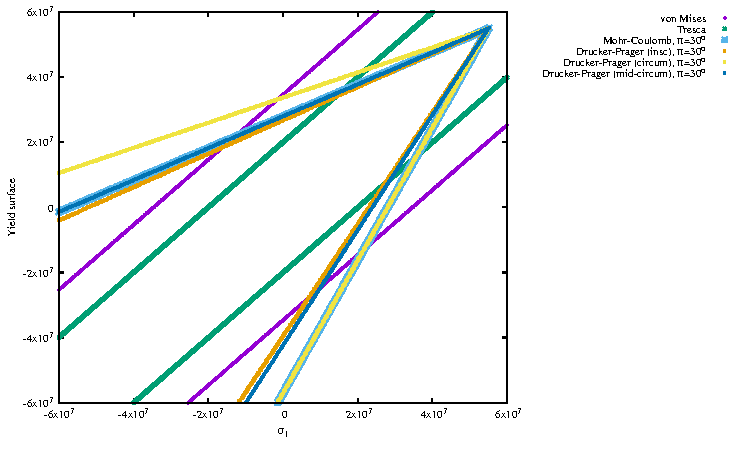
\includegraphics[width=12cm]{images/rheology/surfaces/surfaces_xy.pdf}
\end{center}
We see that the von Mises and Tresca envelopes are parallel to the line $\sigma_1=\sigma_2=\sigma_3$ (which 
is expected since they do not depend on pressure).

The second plot is in the plane $\sigma_1+\sigma_2+\sigma_3=0$ which is perpendicular to the middle line 
$\sigma_1=\sigma_2=\sigma_3=0$. To facilitate plotting the envelopes are plotted as a function of $\sigma_1$ only (so that even though they are circles in the chosen plane they appear here as ellipses):

\begin{center}
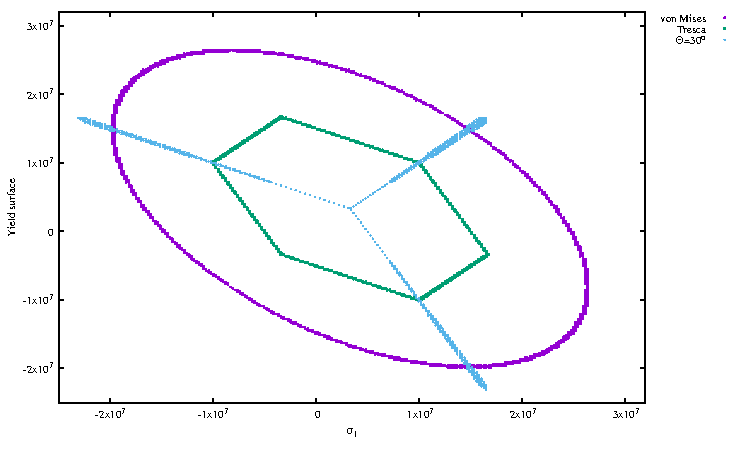
\includegraphics[width=12cm]{images/rheology/surfaces/surfaces_plane2.pdf}
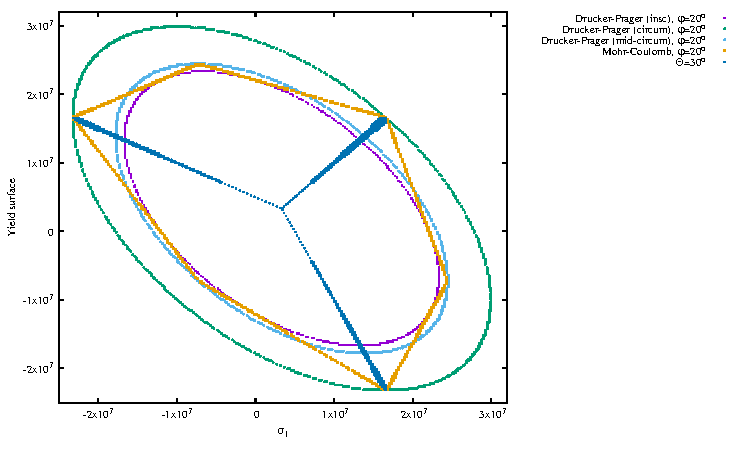
\includegraphics[width=12cm]{images/rheology/surfaces/surfaces_plane.pdf}
\end{center}

We see that we indeed recover that the three Drucker-Prager formulations 
inscribe (purple), middle-circumscribe (blue) and circumscribe (green) the 
Mohr-Coulomb one. 



\newpage
%------------------------------
\subsubsection{Peierls creep}
\index{general}{Peierls creep}
\index{general}{Peierls creep}
\begin{flushright} {\tiny {\color{gray} peierls.tex}} \end{flushright}
%~~~~~~~~~~~~~~~~~~~~~~~~~~~~~~~~~~~~~~~~~~~~~~~~~~~~~~~~~~~~~~~~~~~~~~~~~~~~~~~~~~~~~~~~~~~~~~~~~~

Looking at the literature, there seem to be many formulations for the Peierls creep deformation
mechanism, but it it appears that a standard formulation for the Peierls creep writes:
\[
\dot{\varepsilon} = A \sigma^n \exp \left[ -\frac{Q+pV}{RT} \left(1-(\frac{\sigma}{\sigma_P})^k\right)^q  \right]
\]
and it seems common to take $k=1$, and $n=2$ \cite{gery10,kaka08}
\[
\dot{\varepsilon} = A \sigma^2 \exp \left[ -\frac{Q+pV}{RT} \left(1-\frac{\sigma}{\sigma_P}\right)^q  \right]
\]
Elbeshausen \& Melosh (2018) \cite{elme18} use 
\[
\dot{\varepsilon} = A  \exp \left[ -\frac{Q}{RT} \left(1-\frac{\sigma}{\sigma_P}\right)^q  \right]
\]
In Chenin \etal (2019) \cite{chmd19} the authors state that their Peierls creep implementation
relies on parameters from Evans and Goetze (1979) \cite{evgo79} using the approach of 
Kameyama \etal (1999) \cite{kayk99}:
\[
\eta^{pe}=\frac{2}{3} \frac{(1-s)/s}{(1+s)/2s} A \; (\varepsilon_e^{ds})^{\frac{1}{n}-1} 
\]
with $A$ for this formulation:
\[
A = \left[ A_p \exp \left( -\frac{Q(1-\gamma)^2}{RT} \right)  \right]^{-1/s} \gamma \sigma_p
\]
where $s$ is an effective stress exponent that depends on the temperature:
\[
s = 2 \gamma \frac{Q}{RT} (1-\gamma)
\]
where $\gamma$ is a fitting parameter. 


\Literature 
\textcite{basv06},
\textcite{buro11},
\textcite{faff11},
\textcite{gagd14},
\textcite{gery10},
\textcite{goev79},
\textcite{kaka08},
\textcite{kako09},
\textcite{kary01},
\textcite{mesk10},
\textcite{zhwa13},
\textcite{chsm18},
\textcite{shwl17},
Review article from 1966: Guyot \& Dorn \cite{gudo67}





%-------------------------------------------------
\subsubsection{Stress limiting rheology}

Taken from van Hunen \etal (2002) \cite{vavv02}:
\[
\eta_y = \tau_y \dot{\varepsilon}_y^{-1/n_y} \dot{\varepsilon}_e^{(1/n_y) -1 } 
\]
where the yield stress $\tau_y$, the yield strain rate $\dot{\varepsilon}_y$ and the yield exponent $n_y$ are
prescribed parameters. In this article, $n_y=10$, $\dot{\varepsilon}_y=10^{-15}\si{\per\second}$
When $n_y=1$ the viscosity is constant and given by $\eta_{eff} = \tau_y / \dot{\epsilon}_y$.

This rheology has also been coined pseudo-plastic in Zhong \etal (1998) \cite{zhgm98}. 
Their equation is simply  
\[
\eta_{eff} = A^{1/n} \dot{\varepsilon}_e^{-1+1/n}
\]
where $A$ is the preexponent which depends on temperature, pressure, and composition.
\begin{center}
\includegraphics[width=5.5cm]{images/rheology/zhgm98}
\includegraphics[width=5.8cm]{images/rheology/pseudoplastic/stress}
\includegraphics[width=5.8cm]{images/rheology/pseudoplastic/eta_eff}\\
{\captionfont Left figure is taken from \cite{zhgm98}. Authors report $A=7.9\cdot 10^{-8} \si{\pascal^3\second}$ 
for the $n=3$ case, which makes no sense. See gnuplot script for actual values of $A$.}
\end{center}




%-------------------------------------------------
\subsubsection{Arrhenius law}
\index{general}{Arrhenius law}

A purely temperature-dependent dimensional Arrhenius law that emulates the temperature
dependence of viscosity in silicate rock is often employed for mantle rocks 
\cite{albe00,zhzm09,vata11,bogs13b,namu13,stha13,boba19,gult19}:
\begin{equation}
\eta(T)=\eta_0 \exp \left( \frac{Q}{R}(\frac{1}{T}-\frac{1}{T_0}) \right)
\qquad 
{\rm or}
\qquad 
\eta(T)=\eta_0 \exp \left( \frac{Q}{RT} \right)
\end{equation}
where $\eta_0$ is a reference viscosity and $T_0$ its corresponding reference 
temperature.

It can also account for pressure effects as in \cite{lorg18} where the
diffusion creep viscosity (under the assumption of homogeneous grain size)
is temperature- and pressure-dependent:
\[
\eta(T)=\eta_0 \exp \left( \frac{1}{R}(\frac{Q-pV}{T}-\frac{Q}{T_0}) \right)
\]
(I find the minus sign rather suspicious)



%-------------------------------------------------
\subsubsection{Simple parametrisation of the mantle}

Many CITCOMs-based publications \cite{bumb10,budt14} 
have used the following (dimensionless) viscosity for the mantle:
\[
\eta(T,z) = \eta_r(r) \exp(A(0.5-T))
\]
where $\eta_r$ is a depth-dependent viscosity profile (usually defined as 
discontinuous linear profiles for various shells)

The non-dimensional activation coefficient is chosen to be $A=9.2103$ in 
\cite{budt14} which leads to a temperature-induced viscosity contrast of $10^4$ (for 
$T\in[0,1]$).

This is also called the Frank-Kamenetskii flow rule, as used in \cite{stha13,lemh17}:
\[
\eta' = \eta_0 \exp(-\theta T)
\]
where the the parameters $\eta_0$, $\theta$ account for the local chemical composition of the rock.
Note that the Frank-Kamenetskii approximation takes many forms in the literature \cite{nobr13}.
\index{general}{Frank-Kamenetskii}

Another temperature-dependent common expression is as follows \cite{flyu84}:
\[
\eta(T)=\eta_\infty \exp \left( \frac{Q}{R}(\frac{1}{T}-\frac{1}{T_\infty} ) \right)
\]
Also, following \cite{flyu84}: For studying transient convection in a non-
Newtonian rheological fluid, it is expedient from a
computational point of view to employ a law
which behaves linearly for low stresses initially
and becomes gradually non-Newtonian only after
a certain threshold stress level has been surpassed \cite{chri84,chyu84}:
\[
\eta(T,p,\tau_2) =\eta(T,p) \frac{1}{A_2 + A_3 \tau_2^2}
\]
where $A_2$ is a parameter describing the linear creep
at low stress levels and $A_3$ governs the transition
stress between Newtonian and non-Newtonian rheologies.

Coltice and Sheppard (2018) \cite{cosh18} use a depth- and temperature-dependent 
viscosity formulation:
\[
\eta(z,T)=\eta_0(z) \exp \frac{Q}{RT}
\]
Note that this expression is supplemented with a pseudo-plastic formulation \cite{roct12}.

\Literature: \cite{king16}

%-------------------------------------------------
\subsubsection{Glen's law for ice}\label{ss:glen}


Ice and rocks share similarities in terms of (viscous) rheology.
Glen's law is the most commonly used flow law for ice in glaciers and ice sheets \cite{glen55}
and it is actually a power-law type rheology:
\[
\dot{\bm \varepsilon} = A {\bm \tau}^n 
\]
with $n\sim 3$ and $A\sim 2.4\cdot 10^{-24} \text{Pa}^{-3}\cdot \text{s}^{-1}$ at $0\degree$C.
The effective viscosity is then given by
\[
\eta = \frac{1}{2 A \tau_e^{n-1}} 
\]
\begin{center}
\includegraphics[height=5cm]{images/rheology/glen}
\includegraphics[height=5cm]{images/rheology/goko01}\\
{\captionfont Left: Taken from Glen \cite{glen55}; Right: taken from \cite{goko01}.}
\end{center}
Most of these studies suggest values of the power-law exponent $n\sim 2-4$, and there seems to be 
a general indication that the exponent is lower at lower stresses.

The $A$ coefficient above has been found to depend on temperature and is reasonably described 
with an Arrhenius law:
\[
A(T)=A_0 \exp\left( -\frac{Q}{RT} \right)
\]
A standard formulation is the Paterson-Budd law with a fixed Glen exponent $n=3$ and 
a split Arrhenius term \cite{pabu82}:
\[
A=3.615 \cdot 10^{-13} \text{Pa}^{-3}\cdot \text{s}^{-1}, 
\qquad Q=60 \; \text{kJ}/\text{mol}, \qquad if\quad T<263\text{K} 
\]
\[
A=1.733\cdot 10^{3} \text{Pa}^{-3}\cdot \text{s}^{-1}, 
\qquad  Q=139 \; \text{kJ}/\text{mol}, \qquad if\quad T>263\text{K}
\]
Be careful that in these two equations the temperature $T$ is the pressure-adjusted 
temperature \cite{pabu82}.
Note that $A$ is also affected by the water content and the presence of impurities. 

Finally, Glen's law is the standard rheology used for ice-sheet modelling 
but it does not account for the complex evolution of fabric and resulting anisotropy.
Indeed the grain size evolution (growth \& reduction)
plays a large role in the rheology \textcite{begh21} (2021).
See \stone~59. 


\Literature 
\textcite{grev97} (1997),
\textcite{grbl09} (2009),
\textcite{issg15} (2015),
\textcite{krab16} (2016),
\textcite{jidb17} (2017),
\textcite{heah18} (2018),
Very mathematics heavy papers: \cite{jora11,chgp13}.















%...........................................
\subsubsection{Strain rate partitioning across deformation mechanisms}\label{ss:srpart}
\index{general}{Strain rate partitioning}

When multiple viscous deformation mechanisms are present, one needs more dashpots, and 
more complicated element diagrams than the ones above occur (also when adding plastic deformation).
Two important rules are to be remembered:
1) for parallel components, stresses are additive, strain rates are equal in each; 
2) for components in series, stresses are equal in each and strain rates are additive. 

Let us then look at various assemblies of dashpots and plastic elements:

\begin{itemize}
\item \underline{two viscous dampers in series:} 

\begin{center}
\input{tikz/tikz_dashpotdashpot_series}
\end{center}

each is subjected to the same stress $\tau$ but deforms 
with its own strain rate $\dot{\varepsilon}_1$ and $\dot{\varepsilon}_2$ and we have 
\begin{equation}
\dot{\varepsilon}_T 
= \dot{\varepsilon}_1 + \dot{\varepsilon}_2
= \frac{\tau}{2\eta_1} + \frac{\tau}{2\eta_2}
\end{equation}
The effective viscosity of this combination is denoted $\eta_{eff}$ and is such that 
$\eta_{eff}=\tau/2\dot{\varepsilon}_T$, which means that 
\[
\frac{\tau}{2\eta_{eff}} = \frac{\tau}{2\eta_1} + \frac{\tau}{2\eta_2}
\]
or, 
\[
\eta_{eff}= \left( \frac{1}{\eta_1} + \frac{1}{\eta_2} \right)^{-1}
\]
i.e. it follows that the effective viscosity of two or more viscous dampers in series is the harmonic 
average of the individual viscosities of the dampers.

In general, for n dampers in series:
\[
\eta_{eff}= \left( \sum_{i=1}^n \frac{1}{\eta_i} \right)^{-1}
\]




\item \underline{two viscous dampers in parallel:}

\begin{center}
\input{tikz/tikz_dashpotdashpot_parallel}
\end{center}
 
each is deformed with the same strain rate $\dot{\varepsilon}_T$
and their stresses add up:
\[
\tau = \tau_1 + \tau_2 = 2 \eta_1 \dot{\varepsilon}_T  + 2 \eta_2 \dot{\varepsilon}_T
\]
and since we define the effective viscosity as $\tau = 2 \eta_{eff} \dot{\varepsilon}_T$ then it follows:
\[
2 \eta_{eff} \dot{\varepsilon}_T = 2 \eta_1 \dot{\varepsilon}_T  + 2 \eta_2 \dot{\varepsilon}_T
\]
or, 
\[
\eta_{eff} = \eta_1 + \eta_2 
\]
i.e., the effective viscosity of two or more viscous dampers is the sum of their viscosities ({\sl 
but not their arithmetic mean!}).


\item \underline{one viscous damper and a plastic element in parallel}:
\begin{center}
\input{tikz/tikz_vp}
\end{center}

The effective 'plastic' viscosity of the plastic element is $\eta_p =  \frac{Y}{2 \dot{\varepsilon}_T}$ so 
the effective viscosity of this setup is then  
\[
\eta_{eff} = \frac{Y}{2 \dot{\varepsilon}_T}+\eta_m
\]
which is the viscosity of a Bingham fluid (see Section~\ref{sec:bingham}).


\item \underline{two viscous dampers and a plastic element} arranged as follows:
\begin{center}
\begin{tikzpicture}
%\draw[fill=gray!23,gray!23](0,0) rectangle (7,5);
%\draw[step=0.5cm,gray,very thin] (0,0) grid (12,5); %background grid

\node[] at (0.1,2.7) {$\tau$};
\draw[line width=1mm] (0.5,1.5) -- (0.5,3.5) ;   
\draw [->] (0,2.5) -- (0.45,2.5);
\draw [->] (0,2) -- (0.45,2);
\draw [->] (0,3) -- (0.45,3);

\draw[thick] (0.5,2.5) -- (2,2.5) ;   
\draw[thick] (2.5,2.5) -- (5,2.5) ;   
\draw[thick] (5.5,2.5) -- (7.5,2.5) ;   
\draw[thick] (10.5,2.5) -- (12,2.5) ;   

% v damper
\draw[thick] (1.5,3) -- (2.5,3) -- (2.5,2) -- (1.5,2);  
% ds damper
\draw[thick] (4.5,3) -- (5.5,3) -- (5.5,2) -- (4.5,2);  
% m damper
\draw[thick] (8.5,4) -- (9.5,4) -- (9.5,3) -- (8.5,3);  

\node[] at (2,1.6) {$\eta_{\color{orange}v}$};
\node[] at (5,1.6) {$\eta_{\color{green}ds}$};
\node[] at (9,4.4) {$\eta_m$};

\draw[thick] (9,3.5) -- (7.5,3.5) -- (7.5,1.5) -- (8,1.5);  
\draw[thick] (9.5,3.5) -- (10.5,3.5) -- (10.5,1.5) -- (10,1.5);  

\draw[thick] (8,1.5) -- (8.5,1.4) -- (9.5,1.4) ;   
\draw[thick] (8.5,1.6) -- (9.5,1.6) -- (10,1.5) ;   

\node[] at (9,1.92) {$Y$};

%wall
\draw[line width=2mm] (12,1.5) -- (12,3.5) ;   
\draw[thick] (12,1.5) -- (12.25,1.75) ;   
\draw[thick] (12,1.75) -- (12.25,2) ;   
\draw[thick] (12,2) -- (12.25,2.25) ;   
\draw[thick] (12,2.25) -- (12.25,2.5) ;   
\draw[thick] (12,2.5) -- (12.25,2.75) ;   
\draw[thick] (12,2.75) -- (12.25,3) ;   
\draw[thick] (12,3) -- (12.25,3.25) ;   
\draw[thick] (12,3.25) -- (12.25,3.5) ;   

\draw[>=triangle 45, <->] (0.5,0.95) -- (3.5,0.95);
\draw[>=triangle 45, <->] (3.5,.95) -- (6.5,0.95);
\draw[>=triangle 45, <->] (6.5,0.95) -- (12,0.95);
\node[] at (2,0.75)   {$\dot\varepsilon_{\color{orange}v}$};
\node[] at (5,0.75)   {$\dot\varepsilon_{\color{green}ds}$};
\node[] at (9.5,0.75) {$\dot\varepsilon_{\color{blue}vp}$};

\end{tikzpicture}

\end{center}
This rheology would be called visco-viscoplastic.
The algorithm goes then as follows:
\begin{enumerate}
\item Assume we know $\eta_v$ and $\dot\varepsilon_T$ (from previous iteration), as well as the plasticity parameters $Y$ and $\eta_m$.
\item if $2 \eta_v \dot\varepsilon_T < Y$ the stress is below the yield stress value and plasticity is not active. Use $\eta_v$ in the material model and $\dot\varepsilon_v=\dot\varepsilon_T$.

\item if $2 \eta_v \dot\varepsilon_T > Y$ the stress is above the yield value, which is not allowed. In this case the plastic element is 'switched on'. In that case the viscous damper is in series with the (visco)plastic element. The former deforms with a strain rate $\dot\epsilon_v$ while the latter with $\dot\epsilon_{vp}$ (both under the same stress $\tau$) and we have  $\dot\varepsilon_T = \dot\varepsilon_v  + \dot\varepsilon_{vp}$. 

\begin{eqnarray}
\dot\varepsilon_T 
&=& \dot\varepsilon_v + \dot\varepsilon_{vp}  \nonumber\\
&=& \dot\varepsilon_v + \frac{\tau}{2 \eta_{vp}} \nonumber\\
&=& \dot\varepsilon_v + \frac{\tau}{2 \left( \frac{Y}{2\dot\varepsilon_{vp}} + \eta_m  \right)} \nonumber\\
&=& \dot\varepsilon_v + \frac{\tau}{2 \left( \frac{Y}{2(\dot\varepsilon_T-\dot\varepsilon_v)}+\eta_m\right)} \nonumber\\
\dot\varepsilon_T - \dot\varepsilon_v 
&=& \frac{\tau}{2 \left( \frac{Y}{2(\dot\varepsilon_T-\dot\varepsilon_v)}+\eta_m\right)} \nonumber\\
2 (\dot\varepsilon_T - \dot\varepsilon_v)
\left( \frac{Y}{2(\dot\varepsilon_T-\dot\varepsilon_v)}+\eta_m\right) &=& \tau \nonumber\\
Y +  2(\dot\varepsilon_T - \dot\varepsilon_v) \eta_m &=& \tau \nonumber\\
Y +  2(\dot\varepsilon_T - \frac{\tau}{2 \eta_v}) \eta_m &=& \tau \nonumber\\
Y +  (2\eta_v \dot\varepsilon_T - \tau) \frac{\eta_m}{\eta_v} &=& \tau \nonumber\\
Y +  2\eta_m \dot\varepsilon_T  &=& \tau (1 + \frac{\eta_m}{\eta_v} ) \nonumber
\end{eqnarray}
and finally 
\begin{equation}
\tau  = \frac{Y + 2 \eta_m \dot\varepsilon_T} {1+ \frac{\eta_m}{\eta_v} }
\end{equation}
Note that this solution exists even when $\eta_m=0$, and then rather logically $\tau=Y$.

\item Once we have $\tau$, we can easily compute $\dot\epsilon_v = \frac{\tau}{2\eta_v}$

\item We then compute $\dot\varepsilon_{vp} = \dot\varepsilon_T- \dot\varepsilon_v$ which 
we use to compute $\eta_{vp}$:

\begin{eqnarray}
\eta_{vp} 
&=& \frac{Y}{2\dot\varepsilon_{vp}}+\eta_m \nn\\
&=& \frac{Y}{2(\dot\varepsilon_{T}-\dot\varepsilon_{v})}+\eta_m \nn\\
&=& \frac{Y}{2(\dot\varepsilon_{T}-\frac{\tau}{2\eta_v})}+\eta_m \nn\\
&=& \frac{Y}{2(\dot\varepsilon_{T}- \frac{Y + 2 \eta_m \dot\varepsilon_T} {1+ \frac{\eta_m}{\eta_v} }   
\frac{1}{2\eta_v})}+\eta_m \nn\\
&=& \frac{Y}{2\dot\varepsilon_{T}- \frac{Y + 2 \eta_m \dot\varepsilon_T} {\eta_v + \eta_m}     }+\eta_m \\
&=& \frac{Y(\eta_v+\eta_m)}{2(\eta_v+\eta_m) \dot\varepsilon_{T}- (Y + 2 \eta_m \dot\varepsilon_T) }+\eta_m \\
&=& \frac{Y(\eta_v+\eta_m)}{2 \eta_v \dot\varepsilon_{T}- Y  }+\eta_m \\
&=& \frac{Y(\eta_v+\eta_m)/2\eta_v}{ \dot\varepsilon_{T}- Y/2\eta_v  }+\eta_m 
\end{eqnarray}


\item Having obtained $\eta_{vp}$ we can compute the final effective viscosity
\[
\eta_{eff} = \left( \frac{1}{\eta_v}  + \frac{1}{\eta_{vp}}  \right)^{-1}
\]
\end{enumerate}

On the following plots are shown $\tau$, 
$\dot\varepsilon_{vp}$, $\dot\varepsilon_v$, $\eta_vp$, and $\eta_{eff}$ 
as a function of  $\dot\varepsilon_T$: 

\begin{center}
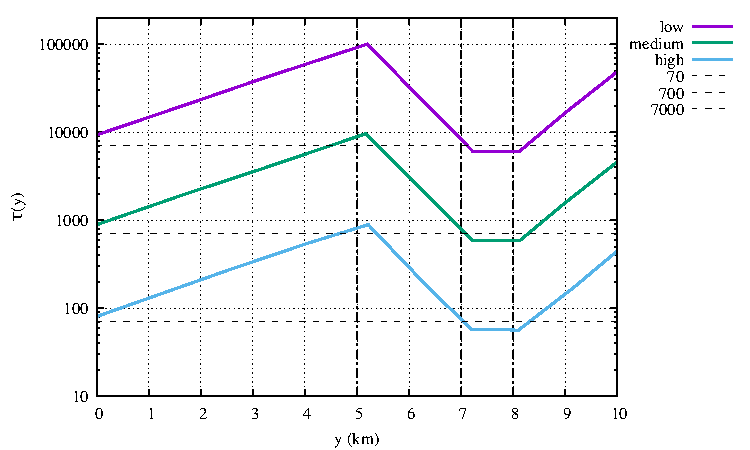
\includegraphics[width=5.5cm]{images/rheology/vvp/tau.pdf}
\includegraphics[width=5.5cm]{images/rheology/vvp/strainrates.pdf}
\includegraphics[width=5.5cm]{images/rheology/vvp/viscosities.pdf}\\
{\captionfont Obtained for $\eta_m=10^{21}$, $Y=20$MPa and $\eta_v=10^{25}$. Python code 
in images/rheology/vvp/}
\end{center}

In the following plots the resulting stress $\tau$ and effective viscosities $\eta_{eff}$
are compared between the above approach ('new') and the simpler (and naive) 
approach where $\dot\varepsilon_T$ 
is used in $\eta_{vp}$ instead of $\dot\varepsilon$ ('old'). In this particular case 
we see that it makes a difference at low strain rates close to the brittle-ductile transition.

\begin{center}
\includegraphics[width=8cm]{images/rheology/vvp/tau_comp.pdf}
\includegraphics[width=8cm]{images/rheology/vvp/viscosities_comp.pdf}\\
{\captionfont Obtained for $\eta_m=10^{21}$, $Y=20$MPa and $\eta_v=10^{25}$. Python code 
in images/rheology/vvp/}
\end{center}

\begin{remark}
The introduction of the damper $\eta_m$ in parallel with the plastic element has an unavoidable
effect: the stress $\tau$ becomes larger than $Y$ at high strain rate values! Since the $vp$ 
block is akin to a bingham fluid, this is no surprise.
\end{remark}

\begin{remark}
The viscous dashpot $\eta_v$ also acts as a maximum viscosity cutoff: if $\eta_{vp}$ becomes (very) large, i.e. $\eta_{vp} \gg \eta_v$, then $\eta_{eff} \rightarrow \eta_v$.
Conversely, if $\eta_p=Y/2\dot\varepsilon_{vp}$ becomes (very) small, i.e. $\eta_p \ll \eta_m$ then $\eta_m$ acts as a minimum viscosity limiter, i.e. $\eta_{vp} \rightarrow \eta_m$. 
Since $\eta_m \ll \eta_v$ then $\eta_{eff} \rightarrow \eta_m$.
\end{remark}

\underline{A simple regularisation} This idea originates in Massmeyer \etal (2013) \cite{madd13}. We postulate
\[
\tilde{\eta}_{eff} = \left(  1 - \exp (- \frac{\dot\varepsilon_T}{\dot\varepsilon_{T}^c}) \right)
\left( \frac{Y}{2 \dot\varepsilon_T} + \eta_m \right)
\]
where $\dot\varepsilon_{T}^c$ is the critical strain  rate at which the transition viscous to 
viscous-viscoplastic occues given by $\dot\varepsilon_{T}^c=Y/2\eta_v$.
When $\dot\varepsilon_{T} \ll \dot\varepsilon_{T}^c$ then the exponential term tends to zero and 
\[
\tilde{\eta}_{eff} \rightarrow  \frac{Y}{2 \dot\varepsilon_T} + \eta_m 
\]
and if $\dot\varepsilon_{T} \rightarrow \infty$ then $\tilde{\eta}_{eff}\rightarrow \eta_m$.
Conversely if $\dot\varepsilon_T \rightarrow 0$ then we can carry out a Taylor expansion of the exponential 
term ($\exp x \sim 1 + x$ when $x$ is small).
\[
\tilde{\eta}_{eff} \sim \left(  \frac{\dot\varepsilon_T}{\dot\varepsilon_{T}^c} \right)
\left( \frac{Y}{2 \dot\varepsilon_T} + \eta_m \right)
\rightarrow 
\frac{\dot\varepsilon_T}{\dot\varepsilon_{T}^c}  \frac{Y}{2 \dot\varepsilon_T}  = \eta_v
\]
At low strain rates the viscosity does not 'explode' but actually converges to the background viscosity $\eta_v$.
The stress $\tau$ corresponding to this viscosity is simply $\tilde{\tau} = 2 \tilde{\eta}_{eff}$. 
Both $\tilde{\tau}$ and $ \tilde{\eta}_{eff}$ are plotted hereunder:


\begin{center}
\includegraphics[width=7.5cm]{images/rheology/vvp/tau_reg.pdf}
\includegraphics[width=7.5cm]{images/rheology/vvp/viscosities_reg.pdf}\\
{\captionfont Obtained for $\eta_m=10^{21}$, $Y=20$MPa and $\eta_v=10^{25}$. Python code 
in images/rheology/vvp/}
\end{center}


\includegraphics[width=7.5cm]{images/rheology/vvp/ratio_visc.pdf}



%which, if  yields the following effective viscosity:
%\[
%\eta_{eff} = \left( \frac{1}{\eta_M}  + \frac{1}{\frac{Y}{2 \dot{\varepsilon}_e} + \eta_m}  \right)^{-1}
%\]
%When the strain rate becomes very small,  $\dot{\varepsilon}_e \rightarrow 0$, $\eta_{eff}\rightarrow \eta_{M}$.
%When the strain rate becomes very large,  $\dot{\varepsilon}_e \rightarrow \infty$, $\eta_{eff}\rightarrow \eta_{m}$.
%We can then rewrite the above equation as a function of $\eta_{min}$ and $\eta_{max}$:
%\[
%\eta_{eff} = \left( \frac{1}{\eta_{max}}  + \frac{1}{\frac{c}{2 \dot{\varepsilon}_e} + \eta_{min}}  \right)^{-1}
%\]
%
%The effective viscosity is plotted here for various values of the minimum viscosity (for $c$=200MPa and $\eta_{max}=10^{25}Pa.s$:
%\includegraphics[width=8cm]{images/viscoplasticity/nu_eff}



\item \underline{two nonlinear viscous dampers in series:} 

\begin{center}
\input{tikz/tikz_dashpotdashpot_series_nl}
\end{center}

There are two dashpots in series, one accounts for dislocation creep, the other for diffusion creep.
The algorithm goes then as follows:
\begin{enumerate}
\item Assume we know $\dot\varepsilon_T$ (from previous iteration). 
\item The dashpots are in series so 
\[
\dot\varepsilon_T = \dot\varepsilon_{ds} + \dot\varepsilon_{df} 
\]
with
\begin{eqnarray}
\dot\varepsilon_{ds}  &=& A_{ds} \tau^n \exp \left(-\frac{Q_{ds}+pV_{ds}}{RT}\right) \label{sr_ds1} \\
\dot\varepsilon_{df}  &=& A_{df} \tau   \exp \left(-\frac{Q_{df}+pV_{df}}{RT}\right) \label{sr_df1} 
\end{eqnarray}
such that we are in fact looking for the stress value $\tau$ so that 
\[
\dot\varepsilon_T = 
A_{ds} \tau^n \exp \left(-\frac{Q_{ds}+p V_{ds}}{RT}\right) 
+
A_{df} \tau   \exp \left(-\frac{Q_{df}+p V_{df}}{RT}\right) 
\]
or, we must find the zero of the function ${\cal F}(\tau)$: 
\[
{\cal F}(\tau) =  \dot\varepsilon_T 
- A_{ds} \tau^n \exp \left(-\frac{Q_{ds}+p V_{ds}}{RT}\right) 
- A_{df} \tau   \exp \left(-\frac{Q_{df}+p V_{df}}{RT}\right) 
\]
This equation can be solved with a Newton-Raphson algorithm
and the iterations will be of the form:
\[
\tau_{n+1} = \tau_n - \frac{{\cal F}(\tau_n)}{{\cal F}'(\tau_n)}
\]
where the derivative of the function ${\cal F}$ with respect to $\tau$ reads:
\[
{\cal F}'(\tau)=\frac{\partial {\cal F}}{\partial \tau}=
- A_{ds} n \tau^{n-1} \exp\left(-\frac{Q_{ds}+pV_{ds}}{RT}\right)
- A_{df} \exp\left(-\frac{Q_{df}+pV_{df}}{RT}\right) 
\]
Once the value of $\tau$ is found, 
the strain rate values of Eqs. (\ref{sr_ds1}) and (\ref{sr_df1})
can be computed and so can the respective effective viscosities:
\begin{eqnarray}
\eta_{ds} 
&=& \frac{1}{2} A_{ds}^{1/n} \dot\varepsilon_{ds}^{\frac{1}{n}-1} \exp \left(\frac{Q_{ds}+pV_{ds}}{nRT}\right) \\
\eta_{df} 
&=& \frac{1}{2} A_{df}^{1/n}  \exp \left(\frac{Q_{df}+pV_{df}}{RT}\right) 
\end{eqnarray}
Their average effective viscosity $\tilde{\eta}_{eff}$ is given by 
\[
\tilde{\eta}_{eff} = \left( \frac{1}{\eta_{ds}} + \frac{1}{\eta_{df}} \right)^{-1}
\]
\end{enumerate}


Rather importantly, as we will see hereafter, the following variant is implemented 
in some codes (e.g. \douar, \fantom, \sopale, and probably many others) 
so as to bypass these costly Newton iterations:
\begin{enumerate}
\item compute $\eta_{ds}$ and $\eta_{df}$ with the {\it same} strainrate $\dot\varepsilon_T$, 
pressure and temperature values
\item average them by means of an harmonic average
\end{enumerate}
In this case, we have
\[
\dot{\varepsilon}_{\color{red} T}= 
A_{df} \tau_{df} \exp\left(-\frac{Q_{df}+pV_{df}}{RT}\right)
\quad\quad\quad
\dot{\varepsilon}_{\color{red} T}= 
A_{ds} \tau_{ds}^n \exp\left(-\frac{Q_{ds}+pV_{ds}}{RT}\right)
\]
or, 
\begin{eqnarray}
\eta_{ds} 
&=& \frac{1}{2} A_{ds}^{1/n} \dot\varepsilon_{\color{red}T}^{\frac{1}{n}-1} \exp \left(\frac{Q_{ds}+pV_{ds}}{nRT}\right) \\
\eta_{df} 
&=& \frac{1}{2} A_{df}^{1/n}  \exp \left(\frac{Q_{df}+pV_{df}}{RT}\right) 
\end{eqnarray}
We see that this simplification has consequences on the dislocation creep viscosity only.


\paragraph{A concrete example}
Let us consider a vertical section of upper mantle, from 660\si{\km} depth to 30\si{\km} depth.
The lithosphere is assumed to be 90\si{\km} thick. The temperature at the moho (the top
of the domain) is set to 550C, 1330C at the LMB and 1380C at the bottom.
A constant strainrate $\dot{\epsilon}_T=10^{-15}\si{\per\second}$ is assumed. 
We assume that the pressure is lithostatic (for simplicity 
the density is taken to be constant at 3300kg/m$^3$).
The temperature and pressure fields are shown hereunder:
\begin{center}
\includegraphics[width=6cm]{images/rheology/effvisc/temperature.pdf}
\includegraphics[width=6cm]{images/rheology/effvisc/pressure.pdf}
\end{center}

Material properties are taken from Karato \& Wu (1993) \cite{kawu93}.
The (fortran) code is available in {\tt images/rheology/effvisc/}.

In what follows, the values obtained with Newton iterations are coined 'NR'
and those obtained without are coined 'CHEAP'.
The diffusion and dislocation creep viscosities can be
computed for both algorithms and are shown hereunder
(As mentioned earlier the diffusion creep viscosity is independent of strain rate so
is the same for both):
\begin{center}
\includegraphics[width=6cm]{images/rheology/effvisc/both_mu_ds.pdf}
\includegraphics[width=6cm]{images/rheology/effvisc/both_mu_df.pdf}
\end{center}
We can also plot the resulting effective viscosity 
$\eta_{eff}$ for both approaches and we see that the differences 
are larger than 20\%. This is shown here under on the left, 
alongside with the partitioning of the strain rate as a function of depth:
\begin{center}
\includegraphics[width=8cm]{images/rheology/effvisc/both_mueff.pdf}
\includegraphics[width=8cm]{images/rheology/effvisc/both_sr.pdf}
\end{center}


























\item \underline{multiple viscous dampers and a plastic element} arranged as follows:



\begin{center}
\input{tikz/tikz_vvp2}
\end{center}



The algorithm goes then as follows:
\begin{enumerate}
\item Assume we know $\dot\varepsilon_T$ (from previous iteration), 
as well as the plasticity parameters $Y$ (a constant in the case of von Mises, or a pressure-dependent 
quantity otherwise) and $\eta_m$.
\item We start by assuming that the plasticity 'block' is not active ($\dot{\varepsilon}_{vp}=0$): we have then three dampers in series. 
We need their associated strain rates 
$\dot{\varepsilon}_{df}$ and $\dot{\varepsilon}_{ds}$ which are such that 
\[
\dot\varepsilon_T = 
\dot\varepsilon_v + \dot\varepsilon_{ds} + \dot\varepsilon_{df} 
\]
with
\begin{eqnarray}
\dot\varepsilon_v &=& \frac{\tau}{2 \eta_v} \label{sr_v} \\
\dot\varepsilon_{ds}  &=& A_{ds} \tau^n \exp \left(-\frac{Q_{ds}+pV_{ds}}{RT}\right) \label{sr_ds} \\
\dot\varepsilon_{df}  &=& A_{df} \tau   \exp \left(-\frac{Q_{df}+pV_{df}}{RT}\right) \label{sr_df} 
\end{eqnarray}
such that we are in fact looking for the stress value $\tau$ so that 
\[
\dot\varepsilon_T = 
A_{ds} \tau^n \exp \left(-\frac{Q_{ds}+p V_{ds}}{RT}\right) 
+
A_{df} \tau   \exp \left(-\frac{Q_{df}+p V_{df}}{RT}\right) 
+
\frac{\tau}{2 \eta_v}
\]
or, we must find the zero of the function ${\cal F}$: 
\[
{\cal F}(\tau) = 
\dot\varepsilon_T 
- A_{ds} \tau^n \exp \left(-\frac{Q_{ds}+p V_{ds}}{RT}\right) 
- A_{df} \tau   \exp \left(-\frac{Q_{df}+p V_{df}}{RT}\right) 
- \frac{\tau}{2 \eta_v} 
\]
This equation can be solved with a Newton-Raphson algorithm
and the iterations will be of the form:
\[
\tau_{n+1} = \tau_n - \frac{{\cal F}(\tau_n)}{{\cal F}'(\tau_n)}
\]
where the derivative of the function ${\cal F}$ with respect to $\tau$ reads:
\[
{\cal F}'(\tau)=\frac{\partial {\cal F}}{\partial \tau}=
- A_{df} \exp\left(-\frac{Q_{df}+pV_{df}}{RT}\right) 
- A_{ds} n \tau^{n-1} \exp\left(-\frac{Q_{ds}+pV_{ds}}{RT}\right)
- \frac{1}{2\eta_v}
\]
Once the value of $\tau$ is found, 
the strain rate values of Eqs. (\ref{sr_ds}), (\ref{sr_df}) and (\ref{sr_v}) 
can be computed and so can the respective effective viscosities:
\begin{eqnarray}
\eta_{ds} 
&=& \frac{1}{2} A_{ds}^{1/n} \dot\varepsilon_{ds}^{\frac{1}{n}-1} \exp \left(\frac{Q_{ds}+pV_{ds}}{nRT}\right) \\
\eta_{df} 
&=& \frac{1}{2} A_{df}^{1/n}  \exp \left(\frac{Q_{df}+pV_{df}}{RT}\right) 
\end{eqnarray}
Their average effective viscosity $\tilde{\eta}_{eff}$ is given by 
\[
\tilde{\eta}_{eff} = \left( \frac{1}{\eta_{ds}} + \frac{1}{\eta_{df}} + \frac{1}{\eta_v} \right)^{-1}
\]


\item if $\tau =2 \tilde{\eta}_{eff} \dot\varepsilon_T < Y$ the stress is below the yield stress value 
and the plasticity element is indeed not active. Use $\tilde{\eta}_{eff}$ in the material model.

\item if $\tau=2 \tilde{\eta}_{eff} \dot\varepsilon_T > Y$ the stress is above the yield value, which is not 
allowed. In this case the plastic element must be present and active and the viscous dampers are then 
in series with the (visco)plastic element. The formers deform 
with a strain rate $\dot{\varepsilon}_v$, $\dot\epsilon_{ds}$ and $\dot{\epsilon}_{df}$ 
while the latter with $\dot\epsilon_{vp}$ (all under the same tress $\tau$) 
and we have  $\dot\varepsilon_T = \dot{\varepsilon}_v + \dot\varepsilon_{ds} + \dot\varepsilon_{df} + \dot\varepsilon_{vp}$ so:

\begin{eqnarray}
\dot\varepsilon_T - \dot{\varepsilon}_v(\tau) - \dot\varepsilon_{ds}(\tau) - \dot\varepsilon_{df}(\tau)  
&=& \dot\varepsilon_{vp}  \nonumber\\
&=& \frac{\tau}{2 \left( \frac{Y}{2\dot\varepsilon_{vp}} + \eta_m  \right)} 
\nonumber\\
%&=&  \frac{\tau}{2 \left( \frac{Y}{2 (\dot\varepsilon_T -\dot{\varepsilon}_v(\tau) -\dot\varepsilon_{ds}(\tau) 
%+ \dot\varepsilon_{df}(\tau)   )} + \eta_m  \right)} 
%\nonumber\\
\dot\varepsilon_T -  \dot{\varepsilon}_v(\tau) -\dot\varepsilon_{ds}(\tau) - \dot\varepsilon_{df}(\tau) 
&=&
\frac{\tau}{2 \left( \frac{Y}{2 (\dot\varepsilon_T -\dot{\varepsilon}_v(\tau) -\dot\varepsilon_{ds}(\tau) 
+ \dot\varepsilon_{df}(\tau)   )} + \eta_m  \right)} \nonumber
\\
2 [\dot\varepsilon_T -\dot{\varepsilon}_v(\tau) -\dot\varepsilon_{ds}(\tau) - \dot\varepsilon_{df}(\tau) ]
 \left( \frac{Y}{2 (\dot\varepsilon_T -\dot{\varepsilon}_v(\tau) -\dot\varepsilon_{ds}(\tau) + \dot\varepsilon_{df}(\tau)   )} + \eta_m  \right) &=& \tau 
\nonumber\\
Y + 2 (\dot\varepsilon_T - \dot{\varepsilon}_v(\tau) -\dot\varepsilon_{ds}(\tau) - \dot\varepsilon_{df}(\tau) ) \eta_m  &=& \tau \nonumber 
\end{eqnarray}
As before, we must find the zero of the function ${\cal F}$: 
\begin{eqnarray}
{\cal F}(\tau) 
&=& Y + 2 [\dot\varepsilon_T -\dot{\varepsilon}_v(\tau)- \dot\varepsilon_{ds}(\tau) -\dot\varepsilon_{df}(\tau) ]\eta_m -\tau \nonumber\\
&=& Y + 2 \left[ 
\dot\varepsilon_T - \frac{\tau}{2\eta_v}-A_{ds} \tau^n \exp \left(-\frac{Q_{ds}+pV_{ds}}{RT}\right) 
- A_{df} \tau   \exp \left(-\frac{Q_{df}+pV_{df}}{RT}\right)  
\right]\eta_m -\tau \nn
\end{eqnarray}
Because dislocation creep involves the $n$-th power of the stress we will here also need 
to find the zero by means of a Newton-Raphson algorithm. 

We have:
\begin{eqnarray}
\frac{\partial {\cal F}}{\partial \tau} &=&
\left[
- \frac{1}{\eta_v} 
-2 \frac{\partial  \dot\varepsilon_{ds}(\tau) }{\partial \tau} 
-2 \frac{\partial  \dot\varepsilon_{df}(\tau) }{\partial \tau} 
\right] \eta_m - 1
\end{eqnarray}

\begin{eqnarray}
{\cal F}(\tau) / 2\eta_m 
&=& 
\frac{Y}{2\eta_m}  + \dot\varepsilon_T 
- \frac{\tau}{2\eta_v}
- A_{ds}(p,T) \tau^n 
- A_{df}(p,T) \tau  
- \frac{\tau}{2\eta_m} \\
&=& 
- A_{ds}(p,T) \tau^n - \left(A_{df}(p,T) +  \frac{1}{2\eta_v} -\frac{1}{2\eta_m} \right) \tau
+ 
\left( \frac{Y}{2\eta_m}  + \dot\varepsilon_T \right) =0
\end{eqnarray}



\end{enumerate}

Note that when $\eta_m=0$ we logically recover $\tau=Y$ as the stress cannot exceed the yield strength $Y$.

Although this approach is probably the most consistent in terms of physics, the presence 
of the Newton-Raphson iterations makes it very expensive since this procedure is to be repeated 
for every quadrature point or every particle.

Let us consider a concrete example: we set $Y=20\si{\mega\pascal}$, $\eta_v=10^{25}\si{pascal}$, 
$\eta_m=10^{20}\si{pascal}$. The domain is one-dimensional of depth $660\si{km}$. The density is
assumed to be constant at $3300\si{\kg\per\cubic\metre}$. Dislocation and diffusion creep parameters
are taken from Karato \& Wu (1993) \cite{kawu93}. The temperature is linear is $20\si{\celsius}$ 
at the surface, $550\si{\celsius}$ at $30\si{km}$ depth, $1330\si{celsius}$ at $90\si{\km}$ depth 
and $1380\si{\celsius}$ at the bottom. Pressure is assumed to be lithostatic. 
The python program and the gnuplot script are in {\sl images/rheology/example}.

In the code I consider two cases: 'old' and 'new'. The latter is described above. 
'old' goes as follows: loop over total strain rate values. 
Compute dislocation and diffusion creep viscosities with it. Compute harmonic 
average of these with linear viscosity. Compute deviatoric stress value. 
use it in dislocation and diffusion formulae to arrive at respective strainrates. 

\newpage
\begin{center}
\includegraphics[width=5.5cm]{images/rheology/example/map_sr_df_old-1}
\includegraphics[width=5.5cm]{images/rheology/example/map_sr_df_new-1}
\includegraphics[width=5.5cm]{images/rheology/example/map_sr_df_diff-1}\\
\includegraphics[width=5.5cm]{images/rheology/example/map_sr_ds_old-1}
\includegraphics[width=5.5cm]{images/rheology/example/map_sr_ds_new-1}
\includegraphics[width=5.5cm]{images/rheology/example/map_sr_ds_diff-1}\\
\includegraphics[width=5.5cm]{images/rheology/example/map_sr_v_old-1}
\includegraphics[width=5.5cm]{images/rheology/example/map_sr_v_new-1}
\includegraphics[width=5.5cm]{images/rheology/example/map_sr_v_diff-1}\\
\includegraphics[width=5.5cm]{images/rheology/example/map_etaeff_old-1}
\includegraphics[width=5.5cm]{images/rheology/example/map_etaeff_new-1}
\includegraphics[width=5.5cm]{images/rheology/example/map_etaeff_diff-1}\\
\includegraphics[width=5.5cm]{images/rheology/example/map_tau_old-1}
\includegraphics[width=5.5cm]{images/rheology/example/map_tau_new-1}
\includegraphics[width=5.5cm]{images/rheology/example/map_tau_diff-1}\\
\includegraphics[width=5.5cm]{images/rheology/example/profile_sr-1}
\includegraphics[width=5.5cm]{images/rheology/example/profile_tau-1}
\includegraphics[width=5.5cm]{images/rheology/example/profile_etaeff-1}\\
\includegraphics[width=5.5cm]{images/rheology/example/map_isplast_old-1}
\includegraphics[width=5.5cm]{images/rheology/example/map_isplast_new-1}\\
{\captionfont Viscous branch: (ds+df+v) 'old' stands 
for the old approach when $\dot{\varepsilon}_T$
was used for all mechanisms. 'new' stands for the new approach and the right strain rate 
decomposition.}
\end{center}



\newpage
\begin{center}
\includegraphics[width=5.5cm]{images/rheology/example/map_etaeff_old_pl-1}
\includegraphics[width=5.5cm]{images/rheology/example/map_etaeff_new_pl-1}
\includegraphics[width=5.5cm]{images/rheology/example/map_etaeff_diff_pl-1}\\
\includegraphics[width=5.5cm]{images/rheology/example/map_tau_old_pl-1}
\includegraphics[width=5.5cm]{images/rheology/example/map_tau_new_pl-1}
\includegraphics[width=5.5cm]{images/rheology/example/map_tau_diff_pl-1}\\
\includegraphics[width=5.5cm]{images/rheology/example/profile_sr_pl-1}
\includegraphics[width=5.5cm]{images/rheology/example/profile_tau_pl-1}
\includegraphics[width=5.5cm]{images/rheology/example/profile_etaeff_pl-1}\\
{\captionfont Visco-viscoplastic rheology: (ds+df+v+vp)} 
\end{center}




\end{itemize}




\begin{remark}
Chenin \etal (2019) \cite{chmd19}, 
base their rheological model on the additive decomposition of the following
deviatoric strain rate tensor ${\bm \varepsilon}^d$:
\[
{\bm \varepsilon}^d =
{\bm \varepsilon}^{el}+
{\bm \varepsilon}^{pl}+
{\bm \varepsilon}^{ds}+
{\bm \varepsilon}^{df}+
{\bm \varepsilon}^{pe}
\]
where the five strain rate terms correspond respectively to the elastic, plastic, 
and viscous creep (dislocation, diffusion, peierls) contributions. 
This implies that all these elements are in series and the associated 
viscosities are then averaged with an harmonic mean. 
Rather interestingly, it is then stated that "this strain rate equation is nonlinear
and solved locally on cell centroids and vertices in order to define the current effective viscosity 
and stress \cite{poso08}."
\end{remark}

\Literature: \cite{hoor89,lopr90,homo90,scps01,lova01,anpa19,elga10}


































%...........................................
\subsubsection{Anisotropic viscosity}

Following the paper by Lev and Hager (2008) \cite{leha08}, 
the anisotropic viscosity enters the equation of momentum through a 'correction'
term added to the isotropic part of the constitutive equation relating
stress and strain rate \cite{mumh02}:
\[
\sigma_{ij} = -p \delta_{ij} + 2 \eta_N \dot{\varepsilon}_{ij}  - 2(\eta_N-\eta_S)\Lambda_{ijkl}\dot{\varepsilon}_{kl} 
\]
where $\eta_N$ is the normal viscosity and $\eta_S$ is the shear viscosity. 
The fourth order tensor $\Lambda$ reflects the orientation of the directors in space, 
denoted by $\vec{n}$:
\[
\Lambda_{ijkl}=\frac{1}{2} (n_i n_k \delta_{lj} + n_j n_k \delta_{il} 
+ n_i n_l \delta_{kj} n_j n_l \delta_{ik} )
- 2 n_i n_j n_k n_l 
\]
Following \cite{modm03,mumh02}, the 'directors' are advected through the model and are 
analogous to particles. The directors are
vector-particles pointing normal to the easy-glide plane or layer,
thus defining the directions associated with $\eta_N$ and $\eta_S$. 
In each time step of the calculation, the directors are advected and rotated by the
flow, and in return determine the viscosity structure for the next time
step \cite{mumc04}.

\begin{center}
\includegraphics[width=10cm]{images/rheology/leha08}\\
{\captionfont Taken from Lev \& Hager (2008) \cite{leha08}.}
\end{center}

\mscthesis\index{general}{MSc Thesis}: redo the Rayleigh-Taylor instabilities with 
anisotropic lithospheric viscosity.
experiments of Lev \& Hager (2008) \cite{leha08}. Look at the three methods 
listed in the other article by 
Lev \& Hager \cite{leha08b}. 
Check Appendix B.2.2 or \cite{perr19} for additional results.

\Literature: 
Richter \& Daly (1978) \cite{rida78},
Saito \& Abe (1984) \cite{saab84},
Vauchez \etal (1998) \cite{vatb98},
M{\"u}lhaus \etal (2002) \cite{mumh02},
M{\"u}lhaus \etal (2003) \cite{mumc03},
M{\"u}lhaus \etal (2004) \cite{mumc04},
Michibayashi \& D. Mainprice (2004) \cite{mima04},
Moresi \& M{\"u}lhaus (2006) \cite{momu06},
M{\"u}lhaus \etal (2010) \cite{mumg10},
M{\"u}lhaus \etal (2011) \cite{muso11},
Sharples \etal (2016) \cite{shmv16},
Perry-Houts \& Karlstrom \cite{peka18},
Kiraly \etal (2020) \cite{kich20}

%...........................................
\subsubsection{Rheology of the lithosphere}

\begin{center}
\includegraphics[height=5cm]{images/rheology/budr08}\\
{\captionfont Schematic view of the three most common first order rheological models of the continental 
lithosphere under a strain rate of 10$^{-14}$s$^{-1}$ . 
In all three models the upper crust has its frictional strength increased with pressure and depth. 
(a) The jelly sandwich model has a weak mid-lower crust and a strong mantle composed of dry olivine. 
(b) The cr\`eme br\^ul\'ee model assumes that the mantle is weak, due to the presence of water and high 
temperature deformation, and the dry and brittle crust determines the strength of the lithosphere. 
(c) The banana split model assumes that the lithosphere as a whole has its strength greatly reduced
due to various strain weakening and feedback processes \cite{budr08}}
\end{center}

\begin{center}
\includegraphics[width=8cm]{images/rheology/bird99}\\
{\captionfont Taken from \cite{bird99}.
Typical vertical distribution of maximum shear stress in continental lithosphere 
undergoing compressional (right) or extensional (left) strain at $10^{-15}$s. 
Friction controls level of shear stress in upper part of crust and sometimes in mantle lithosphere;
then, below brittle/ductile transition, shear stress is controlled by thermally-activated dislocation creep.}
\end{center}

Molnar \cite{moln92} discusses the validity of the Brace-Goetze strength profiles. 
In particular, he has this to say about the power law parameters:
{\it
The uncertainty alone in $Q$ alone renders calculated strengths 
uncertain by 10 times at temperatures of about 700C.
Correspondingly, that uncertainty in Q is approximately equivalent 
to an uncertainty of about 100C in temperature.
}


\begin{center}
\begin{tabular}{l|l}
\hline

Wet Quartzite & upper crust  \cite{jahu12,wabj08} \\
              & upper continental crust \cite{kecw09,cube11} \\
              & lower crust  \cite{jahu12,wabj08} \\
              & ocean sediment \cite{kecw09} \\
Dry Olivine   & lithosphere  \cite{hube07}\\
              & sublithospheric mantle \cite{hube07}\\
Dry Maryland Diabase & lower crust \cite{wabj08,wabj08b} \\
                     & lower continental crust \cite{kecw09,cube11} \\
                     & oceanic crust \cite{wabj08,kecw09,wabj08b,cube11} \\
Wet Olivine   & continental mantle lithosphere \cite{wabj08,wabj08b} \\
              & oceanic mantle lithosphere \cite{wabj08,wabj08b} \\
              & sublithospheric mantle \cite{wabj08,kecw09,wabj08b} \\
              & mantle lithosphere \cite{kecw09} \\
\hline
\end{tabular}
\end{center}



\Literature \cite{buwa06,budr08,rana97a,rana97b}





\todo[inline]{I need to talk about Byerlee's law. \cite{byer78}}

 %--------------------------------------------


\newpage
%------------------------------
\section{The Perzyna model}\label{sec:perzyna}
\index{general}{Perzyna Model}
\begin{flushright} {\tiny {\color{gray} perzyna.tex}} \end{flushright}
%~~~~~~~~~~~~~~~~~~~~~~~~~~~~~~~~~~~~~~~~~~~~~~~~~~~~~~~~~~~~~~~~~~~~~~~~~~~~~~~~~~~~~~~~~~~~~~~~~~


The Perzyna formulation is mentioned in \url{
https://en.wikipedia.org/wiki/Viscoplasticity}.
It is a rate-dependent plasticity formulation that was proposed in 1966 by Piotr Perzyna \cite{perz66}.
See also \url{https://neml.readthedocs.io/en/dev/vp_flow/perzyna.html}.



In what follows I make use of the approach and notations of Zienkiewicz (1974) \cite{zico74} (and all 
the 1974-75 papers that follow) and the book by Owen \& Hinton \cite{owhi}.

The total strain (rate) is divided into two parts\footnote{Zienkiewicz \cite{zico74} 
adds a third term ${\bm \varepsilon}^0$ which stands for initial/autogenous strain such as due 
to temperature changes but I neglect it in what follows.}:
\[
\dot{\bm \varepsilon} = \dot{\bm \varepsilon}^e + \dot{\bm \varepsilon}^{vp}  
\]
where ${\bm \varepsilon}^e$ stands for the elastic strain tensor and 
${\bm \varepsilon}^{vp}$ stands for the visco-plastic strain tensor.

%Since the tensors are symmetric only 6 of the 9 components are independent and 
%the above relationship is often re-written
%\[
%\vec{\varepsilon} = \vec{\varepsilon}^e + \vec{\varepsilon}^{vp}  
%\]
%with
%\[
%\vec{\varepsilon}=
%\left(
%\begin{array}{c}
%\varepsilon_{xx} \\
%\varepsilon_{yy} \\
%\varepsilon_{zz} \\
%\varepsilon_{xy} \\
%\varepsilon_{xz} \\
%\varepsilon_{yz} 
%\end{array}
%\right)
%\]
%For a linear elastic material 
%\[
%{\vec \varepsilon}^e = {\bm D}^{-1} \cdot {\vec \sigma}
%\]
%where ${\bm D}^{-1}$ is a symmetric elasticity matrix (compliance matrix).




The yield condition is given as 
\[
{\FFF}({\bm \sigma},\kappa) 
= \Psi(\bm\sigma,\dot{\bm \varepsilon}) -Y(\kappa) = 0
\]
with ${\FFF}<0$ denoting the purely elastic region, $\kappa$ is a 
history-dependent hardening/softening parameter and $Y(\kappa)$ is a static yield stress.
$\Psi$ is a function of the stress and/or strain rate invariants.

We borrow from classical viscoplasticity theory (Perzyna (1966) \cite{perz66}, Perzyna (1988) \cite{perz88}) 
the idea of a plastic potential defined as $\QQQ({\bm \sigma})$ and write
\begin{equation}
{\dot{\bm \varepsilon}}^{vp} 
= \gamma \Big\langle
\phi\left( {\FFF} \right) 
\Big\rangle
\frac{\partial \QQQ}{\partial \bm\sigma}
\end{equation}
where $\gamma$ is a positive, possibly time-dependent fluidity parameter. 
Note that sometimes the pseudo-viscosity $\bar{\eta}=\gamma^{-1}$ is defined \cite{zigo74}
so that the equation above writes:
\begin{equation}
{\dot{\bm \varepsilon}}^{vp} 
= \frac{1}{\bar{\eta}} \Big\langle
\phi\left( {\FFF} \right) 
\Big\rangle
\frac{\partial \QQQ}{\partial \bm\sigma}
\end{equation}
${\FFF}$ represents the plastic yield condition.
$\phi(x)$ is a positive scalar-valued monotonic increasing function in the range 
$x>0$ such that $\phi^{-1}(x)$ exists and possess similar properties in the same range. 
The notation $\langle \rangle$ denotes the Macaulay 
brackets\footnote{\url{https://en.wikipedia.org/wiki/Macaulay_brackets}} and stands 
for\footnote{there is a difference between 
\cite{zico74}(1974) and \cite{zico74b}(1974) wrt $>$ and $\ge$, and also 
a difference with wikipedia!} 
\begin{eqnarray}
\langle \phi(x) \rangle = \phi(x) & {\rm if} & x>0 \nonumber\\
\langle \phi(x) \rangle = 0 & {\rm if} & x\le 0 \nonumber
\end{eqnarray}
If ${\QQQ}={\FFF}$ then we speak of an {\it associative} law and if ${\QQQ} \neq {\FFF}$ 
we have a {\it non-associative} situation. 
The tensor $\frac{\partial \QQQ}{\partial \bm\sigma}$ represents the direction
of plastic flow and when ${\FFF}={\QQQ}$ it is a vector directed normal to the yield surface
at the stress point under consideration. This is potentially problematic in the 
case of the Tresca and Mohr-Coulomb yield surfaces since the normal is not well defined
along the apices of the surfaces (see Section~7.6 of \cite{owhi}).
In the non-associative case, the direction of plastic flow in the 
principal  stress space during plastic flow is not the same
as the direction of the vector normal to the yield surface.

In what follows we concentrate our attention on isotropic materials for which 
both ${\FFF}$ and ${\QQQ}$ can be defined in terms of stress invariants.

According to Zienkiewicz et al (1975) \cite{zihl75}:
\begin{displayquote}
{\color{darkgray}
One of the main stumbling blocks of the 
classical plasticity theory lay in the universal
assumption, based on Drucker's postulates (Drucker and Prager, 1952), that the plastic 
behaviour is `associated'. With the use of Mohr-Coulomb type yield envelopes to define the
limit between states of elasticity and of continuing irreversible deformation,
the associated behaviour manifestly contradicted observation and gave excessive dilation.
It became necessary therefore to extend plasticity ideas to a `non-associated'
form in which the plastic potential and yield surfaces are defined separately.}
\end{displayquote}
At the same time, it is worth remembering that these early studies mostly dealt
with plasticity in metals, and later soils, but not kilometer-scale crustal layers.

Also, the Perzyna model is not the only one, see for instance
the Duvaut-Lions viscoplastic model or the Consistency model \cite{wasd97,hesd02}.

We therefore need to look into the derivative of the plastic potential ${\QQQ}$
with respect to the stress tensor. Since the potential 
is expressed as a function of the stress invariants ${\III}_1(\bm\sigma)$,
${\III}_2(\bm\tau)$ and $\theta_L(\bm\tau)$, we then have\footnote{
The derivative of the Lod\'e angle was obtained in Section~\ref{ss:lode}}:

\begin{eqnarray}
\frac{\partial \QQQ}{\partial \bm\sigma}
&=&
\frac{\partial }{\partial \bm\sigma} \QQQ\left({\III}_1(\bm\sigma),{\III}_2(\bm\tau),\theta_{\rm L}(\bm\tau)\right)\nn\\
&=&
\frac{\partial \QQQ}{\partial {\III}_1(\bm\sigma)} 
\frac{\partial {\III}_1(\bm\sigma)}{\partial \bm\sigma} 
+
\frac{\partial \QQQ}{\partial \sqrt{{\III}_2(\bm\tau)}} 
\frac{\partial \sqrt{ {\III}_2(\bm\tau)}   }{\partial {\III}_2(\bm\tau)} 
\frac{\partial {\III}_2(\bm\tau)}{\partial \bm\sigma} 
+
\frac{\partial \QQQ}{\partial \theta_{\rm L}(\bm\tau)} 
\frac{\partial \theta_{\rm L}(\bm\tau)}{\partial \bm\sigma} \nn\\
&=&
\frac{\partial \QQQ}{\partial {\III}_1(\bm\sigma)} 
\frac{\partial {\III}_1(\bm\sigma)}{\partial \bm\sigma} 
+
\frac{\partial \QQQ}{\partial \sqrt{{\III}_2(\bm\tau)}} 
\frac{1}{2 \sqrt{ {\III}_2(\bm\tau)}   }
\frac{\partial {\III}_2(\bm\tau)}{\partial \bm\sigma} 
\nn\\
&&
-
\frac{\partial \QQQ}{\partial \theta_{\rm L}(\bm\tau)} 
\frac{\sqrt{3}}{2\cos 3\theta_{\rm L}}
\left[
-\frac32  \frac{ {\III}_3(\bm\tau)   }{ {\III}_2(\bm\tau)^{5/2}}
\; \frac{\partial {\III}_2(\bm\tau)}{\partial \bm\sigma} 
+  \frac{1}{{\III}_2(\bm\tau)^{3/2}} 
\; \frac{\partial {\III}_3(\bm\tau)}{\partial \bm\sigma} 
\right] \nn\\
&=&
\frac{\partial \QQQ}{\partial {\III}_1(\bm\sigma)} 
\; \frac{\partial {\III}_1(\bm\sigma)}{\partial \bm\sigma} 
+  
\left(\frac{\partial \QQQ}{\partial \sqrt{{\III}_2(\bm\tau)}} 
\frac{1}{2 \sqrt{ {\III}_2(\bm\tau)}   }   
+
\frac{\partial \QQQ}{\partial \theta_{\rm L}(\bm\tau)} 
\frac{\sqrt{3}}{2\cos 3\theta_{\rm L}}
\frac32  \frac{ {\III}_3(\bm\tau)   }{ {\III}_2(\bm\tau)^{5/2}}
\right)
\; \frac{\partial {\III}_2(\bm\tau)}{\partial \bm\sigma} \nn\\
&&
-
\frac{\partial \QQQ}{\partial \theta_{\rm L}(\bm\tau)} 
\frac{\sqrt{3}}{2\cos 3\theta_{\rm L}}
\frac{1}{{\III}_2(\bm\tau)^{3/2}} 
\; \frac{\partial {\III}_3(\bm\tau)}{\partial \bm\sigma} \nn\\
&=& 
C_1  \frac{\partial {\III}_1(\bm\sigma)}{\partial \bm\sigma} 
+
C_2  \frac{\partial {\III}_2(\bm\tau)}{\partial \bm\sigma} 
+
C_3  \frac{\partial {\III}_3(\bm\tau)}{\partial \bm\sigma} 
\end{eqnarray}
i.e.
\begin{mdframed}[backgroundcolor=blue!5]
\begin{eqnarray}
\frac{\partial \QQQ}{\partial \bm\sigma}
&=& 
C_1 {\bm a}_1 +
C_2 {\bm a}_2 +
C_3 {\bm a}_3 
=
C_1  \frac{\partial {\III}_1(\bm\sigma)}{\partial \bm\sigma} 
+
C_2  \frac{\partial {\III}_2(\bm\tau)}{\partial \bm\sigma} 
+
C_3  \frac{\partial {\III}_3(\bm\tau)}{\partial \bm\sigma} 
\end{eqnarray}
\end{mdframed}
where the $C_{1,2,3}$ coefficients depend on the plastic potential $\QQQ$
and the stress invariants as follows:
\begin{eqnarray}
C_1 &=&  \frac{\partial \QQQ}{\partial {\III}_1(\bm\sigma)} \\
C_2 
&=& \frac{\partial \QQQ}{\partial \sqrt{{\III}_2(\bm\tau)}} 
\frac{1}{2 \sqrt{ {\III}_2(\bm\tau)}   }   
+
\frac{\partial \QQQ}{\partial \theta_{\rm L}(\bm\tau)} 
\frac{\sqrt{3}}{2\cos 3\theta_{\rm L}}
\frac32  \frac{ {\III}_3(\bm\tau)   }{ {\III}_2(\bm\tau)^{5/2}} \nn\\
&=& 
\frac{\partial \QQQ}{\partial \sqrt{{\III}_2(\bm\tau)}} 
\frac{1}{2 \sqrt{ {\III}_2(\bm\tau)}   }   
-
\frac12
\frac{\tan 3\theta_{\rm L}}{ {\III}_2(\bm\tau)}
\frac{\partial \QQQ}{\partial \theta_{\rm L}(\bm\tau)}  \nn\\
&=& 
\frac{1}{2 \sqrt{ {\III}_2(\bm\tau)}   }   
\left(
\frac{\partial \QQQ}{\partial \sqrt{{\III}_2(\bm\tau)}} 
-
\frac{\tan 3\theta_{\rm L}}{\sqrt {{\III}_2(\bm\tau)}}
\frac{\partial \QQQ}{\partial \theta_{\rm L}(\bm\tau)}  
\right) \nn
\\
C_3 &=&  
-
\frac{\sqrt{3}}{2\cos 3\theta_{\rm L}}
\frac{1}{{\III}_2(\bm\tau)^{3/2}} 
\frac{\partial \QQQ}{\partial \theta_{\rm L}(\bm\tau)} 
\end{eqnarray}
These are identical to those of Eq.~(7.71) in Owen \& Hinton\footnote{This is 
not exactly true: the factor  $\frac{1}{2 \sqrt{ {\III}_2(\bm\tau)} }$
is absent in their Eq.~(7.71) but it is to be found in their Eq.~(7.70).}:
\begin{center}
\fbox{\includegraphics[width=12cm]{images/perzyna/owenhinton2}}
\end{center}

\noindent Note that we already have established (see Section~\ref{ss:recapInv}) that  
\begin{eqnarray}
{\bm a}_1 =\frac{\partial {\III}_1(\bm\sigma)}{\partial \bm\sigma} &=& {\bm 1} \nn\\
{\bm a}_2 =\frac{\partial {\III}_2(\bm\tau)}{\partial \bm\sigma} &=& {\bm \tau} \nn\\
{\bm a}_3 =\frac{\partial {\III}_3(\bm\tau)}{\partial \bm\sigma} 
&=& \bm\tau\cdot\bm\tau -\frac23  {\III}_2(\bm\tau){\bm 1} \nn
\end{eqnarray}
with (we will need these soon)
\begin{eqnarray}
\textrm{Tr}[{\bm a}_1]=
{\rm tr}\left[ \frac{\partial {\III}_1(\bm\sigma)}{\partial \bm\sigma} \right] &=& 3 \\  
\textrm{Tr}[{\bm a}_2]=
{\rm tr}\left[ \frac{\partial {\III}_2(\bm\tau)}{\partial \bm\sigma}   \right] &=& 0 \\
\textrm{Tr}[{\bm a}_3]=
{\rm tr}\left[ \frac{\partial {\III}_3(\bm\tau)}{\partial \bm\sigma}   \right] &=& 
{\rm tr}[\bm\tau\cdot\bm\tau] - 2  {\III}_2(\bm\tau) = 2  {\III}_2(\bm\tau) -2  {\III}_2(\bm\tau) = 0 
\end{eqnarray}

The generic form of the plastic potential derivative then reads 
\begin{mdframed}[backgroundcolor=blue!5]
\begin{eqnarray}
\frac{\partial \QQQ}{\partial \bm\sigma}
&=&
C_1 {\bm 1} 
+
C_2 {\bm \tau} 
+
C_3  \left( \bm\tau\cdot\bm\tau - \frac23  {\III}_2(\bm\tau)  {\bm 1} \right)
\end{eqnarray}
\end{mdframed}

The momentum conservation equation that we solve is 
\[
-\vec\nabla p + \vec\nabla \cdot \left[
2 \eta \dot{\bm\varepsilon}^d(\vec\upnu) 
\right]+ \rho \vec g = \vec 0
\]
so we need the {\it deviatoric} strain rate tensor. 
We here assume for simplicity that there is only a visco-plastic element in the system
(or that the other mechanisms are deviatoric), 
i.e. $\dot{\bm\varepsilon}=\dot{\bm\varepsilon}^{vp}$.
Then 
\begin{eqnarray}
\dot{\bm\varepsilon}^d 
&=& \dot{\bm\varepsilon}^{vp} - \frac13 {\rm tr}[ \dot{\bm\varepsilon}^{vp}] {\bm 1} \nn\\
&=& \gamma \langle \phi(\FFF) \rangle 
\left\{
\left(C_1 {\bm a}_1 + C_2 {\bm a}_2 + C_3 {\bm a}_3 \right)
-\frac13 {\rm tr} \left(C_1 {\bm a}_1 + C_2 {\bm a}_2 + C_3 {\bm a}_3 \right) {\bm 1}
\right\} \nn\\
&=& \gamma \langle \phi(\FFF) \rangle 
\left\{
\left(C_1 {\bm a}_1 + C_2 {\bm a}_2 + C_3 {\bm a}_3 \right)
-\frac13 
C_1 3  {\bm 1}
\right\} \nn\\
&=& \gamma \langle \phi(\FFF) \rangle 
\left\{
\left(C_1 \bm 1 + C_2 \bm\tau + C_3 (\bm\tau\cdot\bm\tau-\frac23 {\III}_2(\bm\tau)\bm 1)\right)
-C_1 \bm 1
\right\} \nn\\
&=& \gamma \langle \phi(\FFF) \rangle 
\left(C_2 \bm\tau + C_3 (\bm\tau\cdot\bm\tau-\frac23 {\III}_2(\bm\tau)\bm 1)\right)
\end{eqnarray}
The $C_{1,2,3}$ coefficients have been computed in 
Sections~\ref{sec:vMcriterion}, \ref{sec:trcriterion}, \ref{sec:dpcriterion} and 
\ref{sec:mccriterion}, and are summarized below: 

\begin{center}
\begin{footnotesize}
\begin{tabular}{lccc}
\hline
& $C_1$ & $C_2(\times \frac{1}{2 \sqrt{{\III}_2({\bm \tau})}})$ & $C_3$ \\
              \hline\hline
Tresca         &0 & $2 \cos\theta_{\rm L} ( 1 + {\color{teal}2} \tan\theta_{\rm L}  \tan 3\theta_{\rm L})$ &
$\frac{\sqrt{3}}{{\III}_2({\bm \tau}) } \frac{\sin\theta_{\rm L} }{\cos 3\theta_{\rm L}}$
\\ \\
von Mises      &0& {\color{teal}1}& 0 \\ \\ 
Mohr-Coulomb   & $\frac13 \sin\phi$ & 
$
\cos \theta_{\rm L} \left[
(1 +  {\color{teal}2}\tan \theta_{\rm L}   \tan 3\theta_{\rm L})
+\frac{1}{\sqrt{3}} \sin\phi
( {\color{teal}2}\tan 3\theta_{\rm L} - \tan\theta_{\rm L}) \right]$
&
$\frac{\sqrt{3}\sin\theta_{\rm L} +  \sin \phi \cos \theta_{\rm L}}
{2 {\III}_2({\bm \tau}) \cos 3\theta_{\rm L}}$ 
\\ \\
Drucker-Prager & $\alpha$ & 1 & 0 \\  
\hline
\end{tabular}
\end{footnotesize}
\end{center}
The differences with the table below  taken from Owen \& Hinton \cite{owhi} are highlighted in blue.
The difference in the von Mises simply comes from the definition of the 
yield value.

\begin{center}
\fbox{\includegraphics[width=12cm]{images/perzyna/owenhinton1}}\\
{\captionfont Taken from \cite{owhi}.
This table supposedly presents all three $C_{1,2,3}$ coefficients 
for all four plastic potentials/yield functions (associative plasticity).
This is however not the case: the $C_2$ column is not $C_2$ but 
$\partial \FFF/\partial\sqrt I_2$!
}
\end{center}


Also, the continuity equation for incompressible flow contains the divergence 
of the velocity field, and in this case 
\begin{eqnarray}
\vec\nabla\cdot\vec\upnu 
&=& {\rm tr}[\dot{\bm\varepsilon}^{vp}]  \nn\\
&=& {\rm tr}\left[ 
\gamma \Big\langle
\phi\left( {\FFF} \right) 
\Big\rangle
\frac{\partial \QQQ}{\partial \bm\sigma}
\right] \nn\\
&=& 
\gamma \Big\langle
\phi\left( {\FFF} \right) 
\Big\rangle
{\rm tr}\left[
C_1  \frac{\partial {\III}_1(\bm\sigma)}{\partial \bm\sigma} 
+
C_2  \frac{\partial {\III}_2(\bm\tau)}{\partial \bm\sigma} 
+
C_3  \frac{\partial {\III}_3(\bm\tau)}{\partial \bm\sigma} 
\right] \nn\\
&=&
\gamma \Big\langle
\phi\left( {\FFF} \right) 
\Big\rangle
{\rm tr}\left[
C_1 {\bm 1} 
+
C_2 {\bm \tau} 
+
C_3  \left( \bm\tau\cdot\bm\tau - \frac23  {\III}_2(\bm\tau)  {\bm 1} \right)
\right] \nn\\
&=&  \gamma \langle \phi(\FFF) \rangle  3 C_1
\end{eqnarray}

%If $C_3=0$, as in the vM or DP case, then we have a relationship between
%deviatoric strain rate and stress that involves a scalar. 
%If not, then a 4th order tensor is needed. This is bad news. 
%Then, vM and Tresca do not modify the continuity equation as $C_1=0$.

I find it difficult to wrap my head around this as the continuity equation 
is usually derived by other means. 
If $C_1$ is not zero, then dilation occurs, the material is not incompressible
so density should also change...  
On the other hand this is a 'problem' only when the bracket is nonzero, i.e. when
plasticity is activated. If the Macaulay bracket is zero, then we recover 
the zero divergence constraint.





\newpage
\section{Moment of inertia} \input{momentofinertia} %-------------------------------------------
\section{The need for numerical modelling}\input{needmodel} %-----------------------------------
\newpage
\section{Important mathematical concepts and equations} \begin{flushright} {\tiny {\color{gray} mathematics.tex}} \end{flushright}
%~~~~~~~~~~~~~~~~~~~~~~~~~~~~~~~~~~~~~~~~~~~~~~~~~~~~~~~~~~~~~~~~~~~~~~~~~~~~~~~~~~~~~~~~~~~~~~~~~~

%------------------------------------
\subsection{Taylor expansion}

\[
f(a+h) = f(a) + h f'(a) + \frac{h^2}{2!} f''(a) + \dots + \frac{h^{n-1}}{(n-1)!}f^{(n-1)}(a)
+ \frac{h^n}{n!}f^{(n)}(a)+ \dots
\]


%------------------------------------
\subsection{Divergence theorem}

This is also coined the Green-Ostrogradski theorem. For a volume $V$ bound by a surface $\Gamma$: 

\begin{mdframed}[backgroundcolor=blue!5]
\begin{equation}
\iint_\Gamma \vec{V}\cdot d\vec{S} = \iiint_V \vec{\nabla}\cdot\vec{V} \; dV
\end{equation}
\end{mdframed}
 \label{ss:maths} %--
